%%%%%%%%%%%%%%%%%%%%%%%%%%%%%%%%%%%%%%%%%%%%%%%%%%%%%%%%%%%%%%%%%%%%
%%%%%%%%%%%%%%%%%%%%%%%%%%%%%%%%%%%%%%%%%%%%%%%%%%%%%%%%%%%%%%%%%%%%
%%                                                                %%
%% An example for writting your thesis using LaTeX                %%
%% Original version by Luis Costa,  changes by Perttu Puska       %%
%% Support for Swedish added 15092014                             %%
%%                                                                %%
%% Esimerkki opinnäytteen tekemisestä LaTeX:lla                   %%
%% Alkuperäinen versio Luis Costa,  muutokset Perttu Puska        %%
%% Ruotsinkielen tuki lisätty 05032014                            %%
%%                                                                %%
%% This example consists of the files                             %%
%% Tähän esimerkkiin kuuluu tiedostot                             %%
%%         thesistemplate.tex (versio 2.0)                        %%
%%         opinnaytepohja.tex (versio 2.0) (for text in Finnish)  %%
%%         aaltothesis.cls (versio 2.0)                           %%
%%         kuva1.eps                                              %%
%%         kuva2.eps                                              %%
%%         kuva1.pdf                                              %%
%%         kuva2.pdf                                              %%
%%                                                                %%
%%                                                                %%
%% Typeset either with                                            %%
%% Kääntäminen joko                                               %%
%% latex:                                                         %%
%%             $ latex opinnaytepohja                             %%
%%             $ latex opinnaytepohja                             %%
%%                                                                %%
%%   Result is the file opinnayte.dvi, which                      %%
%%   is converted to ps format as follows:                        %%
%%   Tuloksena on tiedosto opinnayte.dvi, joka                    %%
%%   muutetaan ps-muotoon seuraavasti                             %%
%%                                                                %%
%%             $ dvips opinnaytepohja -o                          %%
%%                                                                %%
%%   and then to pdf as follows:                                  %%
%%   ja edelleen pdf-muotoon seuraavasti                          %%
%%                                                                %%
%%             $ ps2pdf opinnaytepohja.ps                         %%
%%                                                                %%
%% Or                                                             %%
%% Tai                                                            %%
%% pdflatex:                                                      %%
%%             $ pdflatex opinnaytepohja                          %%
%%             $ pdflatex opinnaytepohja                          %%
%%                                                                %%
%%   Result is the file opinnaytepohja.pdf                        %%
%%   Tuloksena on tiedosto opinnaytepohja.pdf                     %%
%%                                                                %%
%% Explanatory comments in this example begin with                %%
%% the characters %%, and changes that the user can make          %%
%% with the character %                                           %%
%% Selittävät kommentit on tässä esimerkissä varustettu           %%
%% %%-merkeillä ja muutokset, joita käyttäjä voi tehdä,           %%
%% on varustettu %-merkeillä                                      %%
%%                                                                %%
%%%%%%%%%%%%%%%%%%%%%%%%%%%%%%%%%%%%%%%%%%%%%%%%%%%%%%%%%%%%%%%%%%%%
%%%%%%%%%%%%%%%%%%%%%%%%%%%%%%%%%%%%%%%%%%%%%%%%%%%%%%%%%%%%%%%%%%%%

%% Uncomment one of these, if you write in English:
%% the 1st when using pdflatex, which directly typesets your document in
%% pdf (use jpg or pdf figures), or
%% the 2nd when producing a ps file (use eps figures, don't use ps figures!).
\documentclass[english,12pt,a4paper,pdftex,elec,utf8, table]{aaltothesis}

%% To the \documentclass above
%% specify your school: arts, biz, chem, elec, eng, sci
%% specify the character encoding scheme used by your editor: utf8, latin1

%%
%% Käytä toinen näistä, jos kirjoitat suomeksi:
%% ensimmäinen, jos käytät pdflatexia, joka kääntää tekstin suoraan
%% pdf-tiedostoksi (kuvat on oltava jpg- tai pdf-tiedostoina)
%% toinen, jos haluat tuottaa ps-tiedostoa (käytä eps-formaattia kuville,
%% alä käytä ps-muotoisia kuvia!)
%%
%% Use one of these if you write in Finnish:
%%
%\documentclass[finnish,12pt,a4paper,pdftex,elec,utf8]{aaltothesis}
%\documentclass[finnish,12pt,a4paper,dvips]{aaltothesis}

%% Kirjoita y.o. \documentclass optioiksi
%% korkeakoulusi näistä: arts, biz, chem, elec, eng, sci
%% editorisi käyttämä merkkikoodaustapa: utf8, latin1
%%

\usepackage{graphicx}

%% Use this if you write hard core mathematics, these are usually needed
%%
%% Matematiikan fontteja, symboleja ja muotoiluja lisää, näitä tarvitaan usein
\usepackage{amsfonts,amssymb,amsbsy,amsmath}
\usepackage{epigraph}
\usepackage{commath}
\usepackage{listings}
\usepackage{bm}
\usepackage{booktabs}
\usepackage{xcolor}
\usepackage{rotating}
\usepackage{subcaption}
%% Use the macros in this package to change how the hyperref package below
%% typesets its hypertext -- hyperlink colour, font, etc. See the package
%% documentation. It also defines the \url macro, so use the package when
%% not using the hyperref package.
%%
%% Jos et jostain syystä pidä, miten alla oleva hyperref-paketti käyttää
%% fontteja, värejä yms., käytä tämän paketin makroja muuttamaan
%% fonttimäärittelyt. Katso paketin dokumentaatiota. Paketti määrittelee
%% \url-makron, joten ota paketti käyttöön, jos et käytä hyperref-pakettia.
%\usepackage{url}

%% Use this if you want to get links and nice output. Works well with pdflatex.
%%
%% Saat pdf-tiedoston viittaukset ja linkit kuntoon seuraavalla paketilla.
%% Paketti toimii erityisen hyvin pdflatexin kanssa.
\usepackage{hyperref}
\hypersetup{pdfpagemode=UseNone, pdfstartview=FitH,
  colorlinks=true,urlcolor=red,linkcolor=blue,citecolor=black,
  pdftitle={Default Title, Modify},pdfauthor={Samuli Ulmanen},
  pdfkeywords={Modify keywords}}


%% All that is printed on paper starts here
%%
%% Kaikki mikä paperille tulostuu, on tämän jälkeen
\begin{document}

%% Change the school field to specify your school if the automatically
%% set name is wrong
%%
%% Korjaa vastaamaan korkeakouluasi, jos automaattisesti asetettu nimi on
%% virheellinen
% \university{aalto-yliopisto}
% \university{aalto University}
% \school{Sähkötekniikan korkeakoulu}
% \school{School of Electrical Engineering}

%% Only for B.Sc. thesis: Choose your degree programme.
%%
%% Vain kandityölle: Korjaa seuraavat vastaamaan koulutusohjelmaasi
\degreeprogram{Electronics and electrical engineering}
%\degreeprogram{Elektroniikka ja sähkötekniikka}
%%

%% ONLY FOR M.Sc. AND LICENTIATE THESIS: Specify your department,
%% professorship and professorship code.
%%
%% Vain DI/M.Sc.- ja lisensiaatintyölle: valitse laitos,
%% professuuri ja sen professuurikoodi.
\department{Department of Signal Processing and Acoustics}
%\department{Radiotieteen ja -tekniikan laitos}

%\professorship{Digital Signal Processing}
%\professorship{Piiriteoria}
%\code{S3013}
%%

%% Valitse yksi näistä kolmesta
%%
%% Choose one of these:
%\univdegree{BSc}
\univdegree{MSc}
%\univdegree{Lic}

%% Oma nimi
%%
%% Should be self explanatory...
\author{Samuli Y.T. Ulmanen}

%% Your thesis title comes here and again before a possible abstract in
%% Finnish or Swedish . If the title is very long and latex does an
%% unsatisfactory job of breaking the lines, you will have to force a
%% linebreak with the \\ control character.
%% Do not hyphenate titles.
%%
%% Opinnäytteen otsikko tulee tähän ja uudelleen englannin- tai
%% ruostinkielisen abstraktin yhteydessä. Älä tavuta otsikkoa ja
%% vältä liian pitkää otsikkotekstiä. Jos latex ryhmittelee otsikon
%% huonosti, voit joutua pakottamaan rivinvaihdon \\ kontrollimerkillä.
%% Muista että otsikkoja ei tavuteta!
%% Jos otsikossa on ja-sana, se ei jää rivin viimeiseksi sanaksi
%% vaan aloittaa uuden rivin.
\thesistitle{Applying Large-Scale Image Retrieval to Near-Duplicate Image Detection}

\place{Espoo}

%% For B.Sc. thesis use the date when you present your thesis.
%%
%% Kandidaatintyön päivämäärä on sen esityspäivämäärä!
\date{\today}

%% B.Sc. or M.Sc. thesis supervisor
%% Note the "\" after the comma. This forces the following space to be
%% a normal interword space, not the space that starts a new sentence.
%% This is done because the fullstop isn't the end of the sentence that
%% should be followed by a slightly longer space but is to be followed
%% by a regular space.
%%
%% Kandidaattiseminaarin vastuuopettaja tai diplomityön valvoja.
%% Huomaa tittelissä "\" -merkki pisteen jälkeen,
%% ennen välilyöntiä ja seuraavaa merkkijonoa.
%% Näin tehdään, koska kyseessä ei ole lauseen loppu, jonka jälkeen tulee
%% hieman pidempi väli vaan halutaan tavallinen väli.
\supervisor{Assistant Prof.\ Juho Kannala} %{Prof.\ Pirjo Professori}

%% B.Sc. or M.Sc. thesis advisors(s). You can give upto two advisors in
%% this template. Check with your supervisor how many official advisors
%% you can have.
%%
%% Kandidaatintyön ohjaaja(t) tai diplomityön ohjaaja(t). Ohjaajia saa
%% olla korkeintaan kaksi.
%%
\advisor{Lic.Sc.\ (Tech.) Janne Jalkanen}

%% Aalto logo: syntax:
%% Aaltologo: syntaksi:
%%
%% \uselogo{aaltoRed|aaltoBlue|aaltoYellow|aaltoGray|aaltoGrayScale}{?|!|''}
%%
%% Logo language is set to be the same as the document language.
%% Logon kieli on sama kuin dokumentin kieli
%%
\uselogo{aaltoRed}{''}

%% Create the coverpage
%%
%% Tehdään kansilehti
\makecoverpage

%% Note that when writting your master's thesis in English, place
%% the English abstract first followed by the possible Finnish abstract

%% English abstract.
%% All the information required in the abstract (your name, thesis title, etc.)
%% is used as specified above.
%% Specify keywords
%%
%% Kaikki tiivistelmässä tarvittava tieto (nimesi, työnnimi, jne.) käytetään
%% niin kuin se on yllä määritelty.
%% Avainsanat
%%
\keywords{near-duplicate image detection, perceptual hashing,  large-scale image retrieval}

\begin{abstractpage}[english]
  Perceptual hashing outputs an image identifier that can be used for detecting images similar to the original image also known as near-duplicate images. ThingLink is a commercial image annotation service using perceptual hashing for placing annotations from the original annotated image to near-duplicate images. A customer is reporting 20-30\% of near-duplicate images missing annotations. The system is working as expected calling for improved near-duplicate image detection (NDID) methodology.
  We apply Local Features and large-scale image retrieval to near-duplicate image detection. We use a Bag-of-Visual-Words-based image retrieval system for near-duplicate detection by assuming the original image always has the highest score of the images returned by Bag-Of-Visual-Words query. The query always returns the best matching image regardless of how good the match. We employ a cutoff score and classify all queries returning images with scores below the cutoff as \emph{no duplicate found}.
  We show the Local Features and large-scale image retrieval system is better than the perceptual hash-based systems by generating seven different types of near-duplicate image sets from original images in two datasets. The originals form the image database. In addition we use a set of predicted images not in the database to determine how well the systems classify queries as \emph{no duplicate found}. We show the optimal cutoff score to be the maximum score returned while querying predicted negative images for a given dataset. For matching near-duplicates the perceptual hashing schemes use the Hamming Distance, the number of bits by which hashes differ. We find an optimal Hamming Distances for both hashes. Despite tuning, we demonstrate Local Features and large-scale image retrieval to be the superior system for both datasets and all seven types of near-duplicate images used in near-duplicate image detection simulations.



  %% show it to be superior to the currently used simple block mean-based hash and a DCT-based perceptual hash systems by running near-duplicate detection simulations querying two different datasets by sets of seven different types of near-duplicate images.

  %% We show that a Bag-of-Visual-Words based image retrieval system can be used for near-duplicate detection by assuming the original image to always have the highest score of the near-duplicate images returned by Bag-Of-Visual-Words query. Bag-of-Visual-Words always returns the best match regardless of how good the match. We employ a cutoff score and classify all queries returning a lower score as not in the database. We determine the cutoff score to be optimal when set to the maximum score encountered querying predicted negative images. The Hamming Distance, the number of bits by which the hashes differ is optimal all around by setting it to 4 for both perceptual hashes, although if the type of near-duplicate under scrutiny can be further used to choose a better value and depends on the type of hash and the type of duplicate.
  %% Perceptual hashing is a simple way to create an image identifier from an image for use in identifying images very similar to the original otherwise known as near-duplicate images. ThingLink is a commercial image annotation service and uses perceptual hashing for near-duplicate image detection in order to place annotations on all versions of an original annotated image. A customer is reporting 20-30\% of near-duplicate images missing annotation found in the original image. We frame near-duplicate detection as a binary classification problem and apply Local Features and large-scale image retrieval for near-duplicate image detection comparing the results to perceptual hashing. Evaluation of Receiver Operating Characteristic and Precision Recall Curves reveal optimal parameters for perceptual hashing and large-scale image retrieval for near-duplicate image detection as well as Local Features as a better method for detecting dear-duplicate images.
\end{abstractpage}

%% Force a new page so that the possible English abstract starts on a new page
%%
%% Pakotetaan uusi sivu varmuuden vuoksi, jotta
%% mahdollinen suomenkielinen ja englanninkielinen tiivistelmä
%% eivät tule vahingossakaan samalle sivulle
\newpage
%
%% Abstract in Finnish.  Delete if you don't need it.
%%
%% Suomenkielinen tiivistelmä. Poista, jos et tarvitse sitä.
%% Opinnäytteen ostikko suomeksi
\thesistitle{Hajautusfunkion korvaaminen paikallisilla erityispiirteillä kuvien duplikaattitunnistuksessa}
\advisor{Lic.Sc. (Tech.) Janne Jalkanen}
\degreeprogram{Electronics and electrical engineering}
\department{Signaalinkäsittelyn ja akustiikan laitos}
%\professorship{Digitaalinen signaalinkäsittely}
\keywords{hajautusfunktio, paikalliset piirteet, kuvien duplikaattitunnistus}

\begin{abstractpage}[finnish]
Hajautusfunktio on tapa luoda kuvatunniste identifioimaan kuvia, joissa voi esiintyä pieniä poikkeamia alkuperäiseen kuvaan nähden. ThingLink on kaupallinen kuvien annotaatiopalvelu, joka käyttää hajautusfunktioita palvellakseen alkuperäisen kuvan annotaatiot myös kuvaduplikaatteihin. 20-30\% asiakkaan kuvaduplikaateista eivät tunnistu oikein. Tarvitaan parempi metodi kuvien duplikaattitunnistukseen. Sovellamme paikallisia piirteitä ''Bag-of-Visual-Words''-haun kanssa kuvien duplikaattitunnistukseen ja demonstroimme simulaatiolla metodin olevan parempi kuin käytössä olevat hajatusfunkiopohjaiset duplikaattitunnistimet.
\end{abstractpage}

%% Force new page so that the Swedish abstract starts from a new page
\newpage

%% Preface
%%
%% Esipuhe
\mysection{Preface}
Pia, I love you. Thank you for introducing me to coffee. Thank you Tua for being an inspiration! A huge thank you to my parents for taking me to places I didn't want to go and my brother Arttu for going there with me.

Thanks to Janne for sharp guidance over lunches and Assistant Prof.\ Juho Kannala for introducing me to some of the giants in the field of Computer Vision and taking me under his informative instruction.\\

\vspace{5cm}
Otaniemi, \today

\vspace{5mm}
{\hfill Samuli Y.\ T.\ Ulmanen \hspace{1cm}}

%% Force new page after preface
%%
%% Pakotetaan varmuuden vuoksi esipuheen jälkeinen osa
%% alkamaan uudelta sivulta
\newpage


%% Table of contents.
%%
%% Sisällysluettelo
\thesistableofcontents


%% Symbols and abbreviations
%%
%% Symbolit ja lyhenteet
\mysection{Symbols and abbreviations}
%\mysection{Symbolit ja lyhenteet}
\subsection*{Symbols}
%\subsection*{Symbolit}

\begin{tabular}{ll}
$\Delta(q,d)$ & Hamming Distance\\
$\mathcal{C}_s$ & Local Features Classifier cutoff score\\
$\mathcal{C}_{s_{max}}^{-P}$ & The maximum score encountered while querying predicted negative images\\
  $\mathcal{P}$ & Precision\\
  $\mathcal{R}$ & Recall\\
  P & Predicted class in the contingency matrix\\
  $\rho$ & Pearson product-moment correlation coefficient\\
  R & Realization of positive or negative in the contingency matrix\\
  $r_G$ & Matthews correlation\\
  $s_{-P}$ & image score describing fit to database image in the -P-dataset\\
\end{tabular}

\subsection*{Abbreviations A-M}

\begin{tabular}{ll}
  +P & Predicted positive\\
  -P & Predicted negative\\
  +R & Real positive\\
  -R & Real negative\\
  ADC & Asymmetric Distance Computation\\
  AKAZE & Accelerated KAZE features\\
  ANN & Approximate Nearest Neighbor\\
  AOS & Additive Operator Splitting nonlinear diffusion filtering\\
  BBF & Best-Bin-First indexing for ANN\\
  BOF & Bag of Features\\
  BoW & Bag-of-Words representation, also seen used interchangeably with BOF\\
  BRISK & Binary Robust Invariant Scalable Keypoints\\
  DCT & Discrete cosine transform\\
  DoG & Difference of Gaussians\\
  $\epsilon -NN$ & $\epsilon$ - Nearest Neighbor, like ANN\\
  FED & Fast Explicit Diffusion a fast nonlinear diffusion filtering framework\\
  FK & Fisher Kernel\\
  FP & False Positive\\
  FPA & False Positive Average\\
  FPR & False Positive Rate\\
  FN & False Negative\\
  FNA & False Negative Average\\
  FV & Fisher Vector\\
  GMM & Gaussian Mixture Model\\
  IVFADC & inverted file system with asymmetric distance computation\\
  JPEG & lossy compression for digital images by DCT\\
  KAZE & feature detection by local features\\
  k-d tree & k-dimensional tree\\
  K-NN & K-Nearest Neighbor\\
  L2-norm & L2 or $l^2$ normalization. Divide by vector absolute value\\
  LSH & Locality Sensitive Hashing\\
  mAP & mean average precision, a metric for retrieval performance\\
  M-LDB & Modified-Local Difference Binary feature descriptor used in AKAZE features\\
  MLE & Maximum Likelihood Estimation\\
  MultiVLAD & Multiple VLAD descriptors\\
\end{tabular}

\clearpage
\subsection*{Abbreviations N-Z}
\begin{tabular}{ll}
  NDID & Near-Duplicate Image Detection\\
  NN & Nearest Neighbor\\
  ORB & Oriented FAST and Rotated BRIEF fast robust feature detector\\
  OSS & Open Source Software\\
  PCA & Principal Component Analysis\\
  px & A pixel  \\
  PR & Precision-Recall\\
  RGB & red, green, blue color space\\
  ROC & Receiver Operating Characteristic\\
  SDC & Symmetric Distance Computation\\
  SIFT & Scale Invariant Feature Transform \\
  SSR & Signed Square Root normalization\\
  SURF & Sped Up Robust Features \\
  tf-idf & term frequency - inverse document frequency\\
  TP & True Positive\\
  TNR & True Negative Rate\\
  TPR & True Positive Rate\\
  TN & True Negative\\
  UA   & User Agent facilitates end user interaction with Web content (Browser)\\
  UI   & User Interface\\
  URI  & Uniform Resource Identifier aka URL\\
  VLAD & Vector of Locally Aggregated Descriptors\\
\end{tabular}
%% Sivulaskurin viilausta opinn\"aytteen vaatimusten mukaan:
%% Aloitetaan sivunumerointi arabialaisilla numeroilla (ja j\"atet\"a\"an
%% leip\"atekstin ensimm\"ainen sivu tyhj\"aksi,
%% ks. alla \thispagestyle{empty}).
%% Pakotetaan lis\"aksi ensimm\"ainen varsinainen tekstisivu alkamaan
%% uudelta sivulta clearpage-komennolla.
%% clearpage on melkein samanlainen kuin newpage, mutta
%% flushaa my\"os LaTeX:n floatit
%%
%% Corrects the page numbering, there is no need to change these
\cleardoublepage
\storeinipagenumber
\pagenumbering{arabic}
\setcounter{page}{1}


%% Text body begins. Note that since the text body
%% is mostly in Finnish the majority of comments are
%% also in Finnish after this point. There is no point in explaining
%% Finnish-language specific thesis conventions in English. Someday
%% this text will possibly be translated to English.
%%
%% Leip\"ateksti alkaa
\section{Introduction}
\thispagestyle{empty}
Images are a cornerstone of the World Wide Web. ThingLink is a commercial service hosting over 5 million annotated images, such as the Bengtskär lighthouse in figure \ref{bengtskar}, created by students, teachers, journalists, real-estate agents or just about anyone with web access. Customers annotate images with ThingLink and place a ThingLink script on their website containing the annotated images. The script asks ThingLink with an image Universal Resource Identifier (URI) for annotations. Modified versions of the original image are served from a different URI than the original image. These slightly modified versions are called \emph{near-duplicate images} and finding the original for a near-duplicate image is called \emph{near-duplicate image detection} (NDID). NDID has applications ranging from copyright enforcement to identifying image forgeries.  ThingLink uses a perceptual hash as a secondary identifier for linking annotations of the original image to near-duplicate images.

\begin{figure}[htb]
\begin{center}
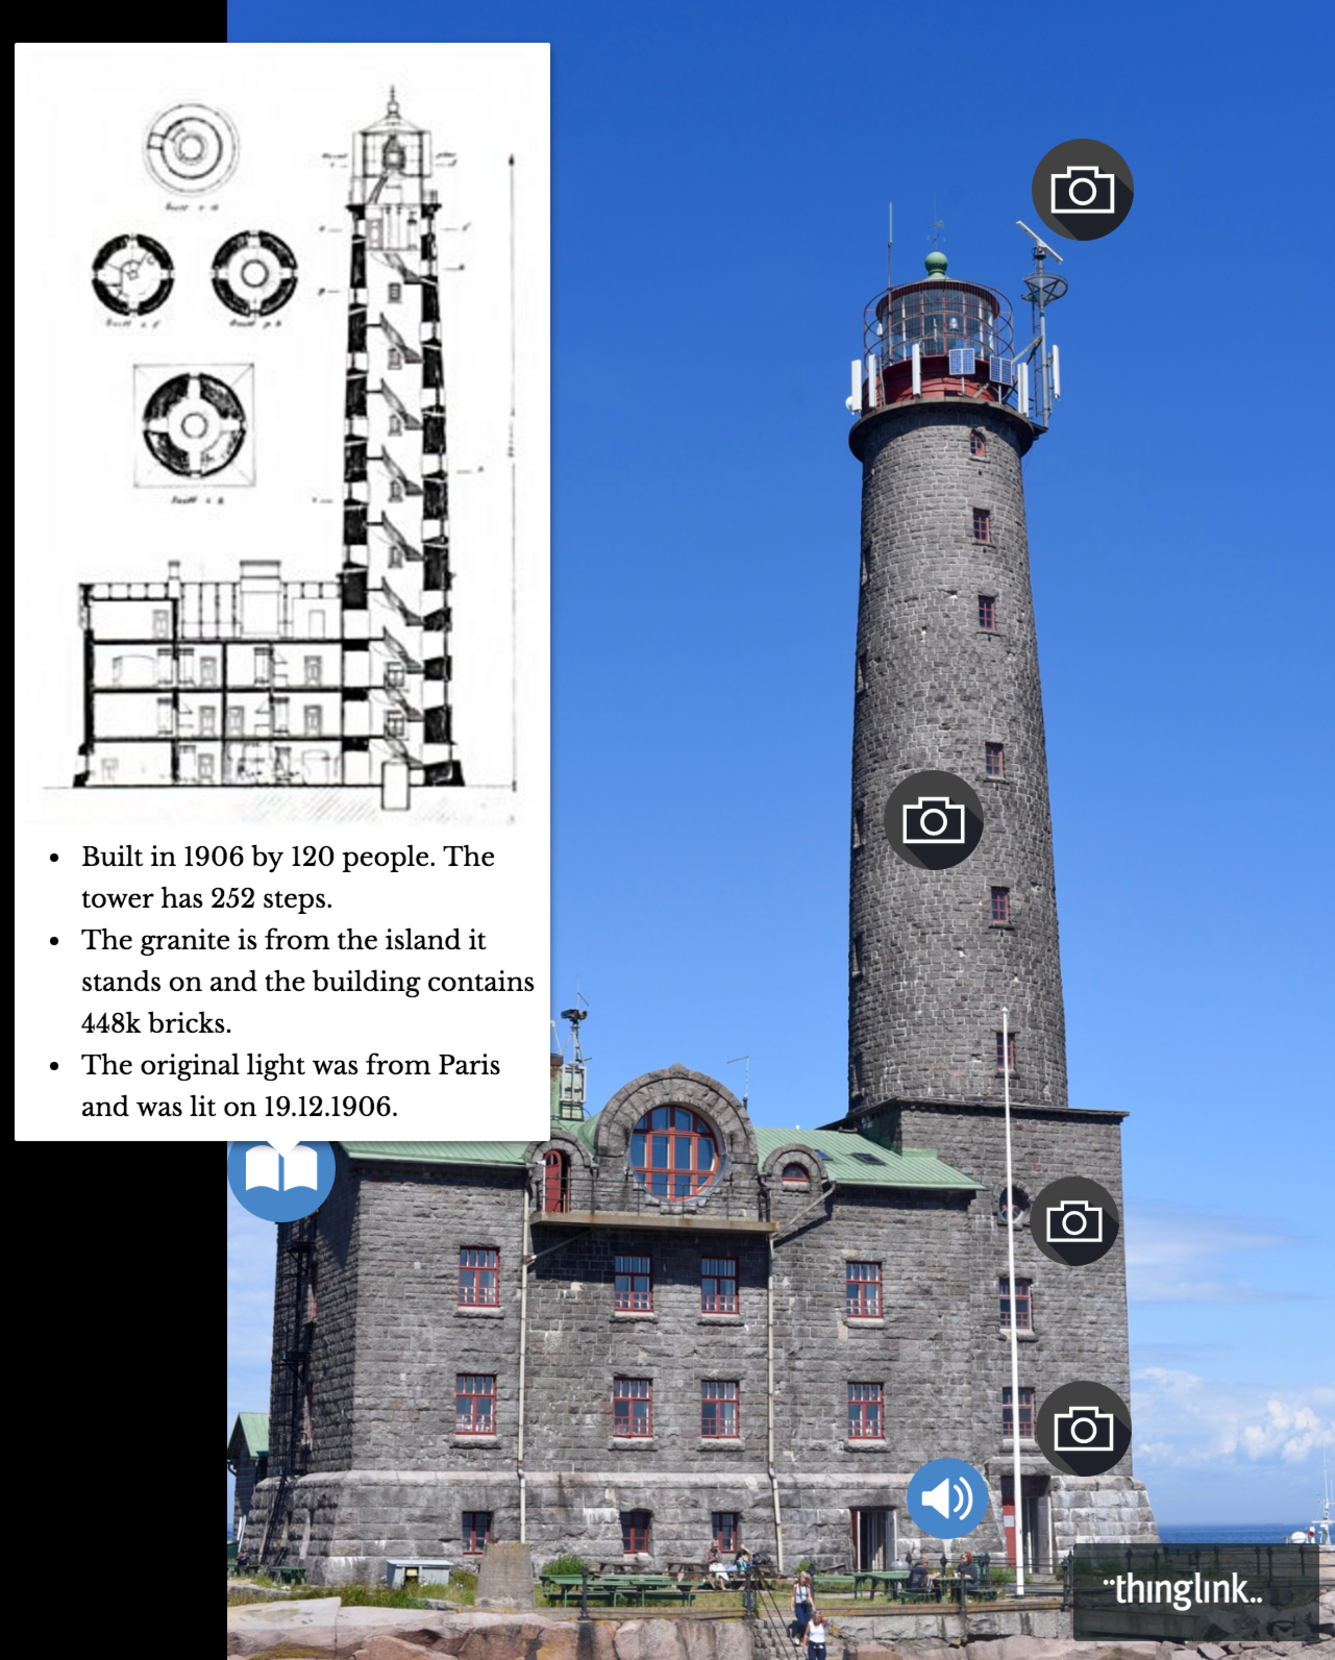
\includegraphics[height=10cm]{figures/bengtskar}
\end{center}
\caption{The Bengtskär lighthouse, the southernmost inhabited building in Finland photographed by the author and annotated with ThingLink. The camera-, audio-, and book icons are image annotations. They may contain text, limited hypertext, images, videos and sound accessible by mouse hover on desktop and touch on mobile. The annotation may also link to a relevant webpage.}
\label{bengtskar}
\end{figure}

\subsection{Problem Setting}
A simple block mean based hash (Simple Hash) and a DCT based hash (DCT Hash) are perceptual hashes used by ThingLink in production. To match near-duplicates to original images, Hamming Distance ($\Delta(q,d)$), the number of bit positions two perceptual hashes differ, is used as a distance function. $\Delta(q,d)=10$ is currently used as recommended in \cite{Zauner2010}. However we do not know if this is the most effective setting.

A customer is reporting 20-30\% false negatives for near-duplicate image detection. When detection fails, annotations do not appear on the near-duplicate image resulting in a loss of service. The near-duplicate detection system is working as expected, so an improved approach is needed. ThingLink requirements for a near-duplicate detector are a high true positive rate (TPR), a high true negative rate (TNR), and a low false positive rate (FPR) for detection of near-duplicate images.

Local Features have been successfully used for detecting near-duplicate images in \cite{Chum2008}, \cite{Chum2010}, \cite{Lee2010} and \cite{dong2012high}. Vedaldi et al.\ demonstrate large-scale image retrieval in \cite{Vedaldi2012} using Local Features detection and description with Bag-of-Visual-Words based retrieval. There Local Features are quantized into visual words from a learned vocabulary. An inverted index is used for efficient matching where each word links to the images it is contained in. Each query into the database returns 10 best matching images.

We apply Local Features and Bag-of-Visual-Words system to near-duplicate image detection by assuming the original image to have the highest score (the number of matching visual words) and picking this image as the near duplicate candidate. As the query always returns an image no matter how bad the match, we employ a cutoff score $\mathcal{C}_s$ below which the duplicate candidate is rejected and the query returns \emph{no duplicate found}. What is a good cutoff score $\mathcal{C}_s$? Is NDID by Local Features and large-scale image retrieval a better system compared to NDID by perceptual hashing employed by ThingLink today?

\subsection{Research Questions}
\begin{itemize}
\item[--] What is a good Hamming Distance $\Delta(q,d)$ for near-duplicate image detection by perceptual hashing?
\item[--] What is a good cutoff score $\mathcal{C}_s$ to return \emph{no near-duplicate match found} for near-duplicate image detection with Local Features and Bag-of-Visual-Words?
    \item[--] Is the highest scoring image with score $s > \mathcal{C}_s$ from a query into an inverted index of Bag-of-Visual-Words the near-duplicate match for the query?
    \item[--] Does Local Features and Bag-of-Visual-Words improve over DCT-, and simple block mean based- perceptual hashes for near-duplicate image detection?
    \item[--] In theory, can Local Features and large-scale image retrieval be deployed at a scale of 5 million images at ThingLink for improved near-duplicate image detection?
\end{itemize}

\subsection{Scope}
This thesis considers near-duplicate image detection excluding all other uses of perceptual hashing, Local Features and large-scale image retrieval. Cryptographic hashing is not considered nor are any uses of perceptual hashing or other methods for digital watermarking. Image category recognition is an interesting topic not in the scope of this thesis. Finding an improved perceptual hashing method is also not in scope of this thesis. We are only interested in determining if the Local Features and large-scale image retrieval based NDID system is better to the currently used systems.

\subsection{Overview}
We review perceptual hashing as it is used at ThingLink today for the description and retrieval of near-duplicate images. A review of state-of-the-art in Local Features detection and description methods and large-scale image retrieval follows. Section \ref{NDID} covers near-duplicate image detection simulations and treating NDID as a binary classification problem as well as the evaluation of binary classifiers. After simulation \emph{Results} in section \ref{results}, we discuss our findings and draw conclusions.

\clearpage

\section{Perceptual Hashing}\label{perceptualhash}
A perceptual hash $H(I)$ of image $I$ is a bit sequence of length $L$ constructed from the image pixels such that similar images have similar hash values and different images have vastly differing hash values. According to \cite{Zauner2010}, perceptual hashing has vast modes of usage from content identification to content-based media retrieval.

In this paper we will only consider the use of a simple block-mean-based hash and a version of DCT-based hash for content based media retrieval, more specifically the retrieval of content annotations. More precisely perceptual hash
\begin{equation}\label{hashfunction}
h = H(I)
\end{equation}
is the result of the hash function $H$ taking the image $I$ as input. $H$ has the properties in table \ref{hashcriteria}.

\def\arraystretch{1.5}
\begin{table}[htb]
\caption{Perceptual hash requirements. \cite{Zauner2010}}
\label{hashcriteria}
\begin{center}
\begin{tabular}{p{0.5\linewidth}}
  \toprule
  $H$ maps from arbitrary size $I$ to fixed number of bits $m$\\
  $H(I)$ fast to compute \\
  $H(I)$ is easy to implement\\
  $H(I)$ is easy to understand\\
  \bottomrule
\end{tabular}
\end{center}\end{table}
In addition, according to \cite{mihccak2001new} given $P$ as probability and $L$ as the length of the hash, the hash function $H(I)$ (eq. \ref{hashfunction}) should
\begin{enumerate}
\item Distribute hashes equally:\\
  \begin{equation}\label{phashdistribute}
  P[H(X)=\alpha]\approx\frac{1}{2^L},\quad\forall\alpha\in \{0/1\}^L
  \end{equation}
\item Visually different images X and Y are pairwise independent: $\forall\alpha,\beta\in\{0/1\}^L$\\
  \begin{equation}\label{phashindependent}
    P[H(X)=\alpha|H(Y)=\beta]\approx P[H(X)=\alpha]
  \end{equation}
\item Approximately equal for visually similar images X, $\hat{X}$\\
  \begin{equation}\label{phashsame}
    P[H(X) = H(\hat{X})] \approx 1
  \end{equation}

\item Be different for visually different images X, Y\\
  \begin{equation}\label{phashdif}
    P[H(X)=H(Y)]\approx 0
  \end{equation}
\end{enumerate}
The distance function used in finding a near duplicate for a perceptual hash in this paper is the Hamming Distance.

\subsection{Block Mean Based Simple Hash}\label{simplehash}
According to \cite[p. 20]{Hadmi2012} the simple hash belongs in the statistic-based hashing schemes and is a simplified version of the block mean value based hash in \cite{Yang2006}. The simple hash (eq. \ref{simplehasheq}) scales the image to 8px $\times$ 8px gray scale. Thresholding takes place where the average value of the most significant byte is found and hash bits are set to one if the image pixel is greater than the average or to zero if it is less than or equal to the average. More specifically the resulting hash has two parts. The most significant 64 bits represent the image pixels and the least significant 64 bits represent the horizontal flip of the 8px $\times$ 8px gray scale image.
\begin{equation} \label{simplehasheq}
  \begin{split}
  b_{i} = 1 | I_{msB}(u,v) > px_{avg}\\
  b_{i} = 0 | I_{msB}(u,v) \leq px_{avg}
  \end{split}
\end{equation}
where $b_{i}$ denotes $i$th hash bit where $0 \leq i < 64$ and $I_{msB}(u,v)$ is the most significant byte of pixel of $I$ at $(u,v)$ where $0 \leq u,v < 8$. The second part (eq. \ref{simplehasheqmirror}) of the hash is calculated on the mirror image of $I$ where $I_{msB}$ denotes the most significant byte of the image RGB pixel value.

\begin{equation} \label{simplehasheqmirror}
  \begin{split}
  b_{i} = 1 | I_{msB}(8-j,v) > px_{avg}\\
  b_{i} = 0 | I_{msB}(8-j,v) \leq px_{avg}
  \end{split}
\end{equation}

A simple hash is easy to understand, implement and fast to calculate so it meets all the criteria in table \ref{hashcriteria}. A single simple hash takes on average 70ms on Matlab 2015a on a Mid 2014 13 inch Macbook Pro. Out of the methods presented in this paper it is the fastest to understand and the fastest to implement. Yet, it should perform well for isotropically scaled images and the thresholding ensures that any uniform change to pixel data where the relationships between the pixels stay the same \cite{Zauner2010}. Any nonuniform changes to pixel values especially relating to moving pixel positions relative to the original image will perform poorly.

Content based image retrieval is done by calculating the hash of an incoming image and comparing it to the image hashes for that user. Typically the number of hashes in the set does not exceed 100. A Hamming Distance is used so the incoming image hash and a hash in the database may differ by $n$ bits where $n$ is the Hamming Distance.

\subsection{DCT-Based Hash}
According to \cite{Gonzalez2002}, many ''transform coding systems are based on the DCT, which provides a good compromise between information packing ability and computational complexity'', properties which are in accordance with requirements for perceptual hashes in table \ref{hashcriteria}. A DCT-based hash (DCT Hash) is formed using a gray scale scaled version of the image, a DCT transform of the scaled image and thresholding to produce a $L=64$ bit hash. Unlike the simple hash, DCT Hash operates in the frequency domain. Especially the low frequency DCT image components are difficult to change without visually altering the image \cite{Fridrich1999}.

To create the hash, the image is reduced to $32$ by $32$ px gray scale. From the result, the most significant byte of the pixel (reduced image) is used. $N=32$ DCT (eq. \ref{dcteq}) is applied to the reduced image and the coefficients are set according to equation \ref{dctcoefeq}.

Using only the $N=8$ (top left corner) of the $N=32$ DCT, the average of the result is calculated and origin result value is discarded as it would throw off the average. The use of average as a threshold is unlike \cite{Coskun2004} where the median is used. The bits of the hash are set to 1 or 0 if the DCT-value is above or below average respectively according to eq. \ref{simplehasheq}.

\begin{equation}\label{dcteq}
T(u,v)= \sum_{u=0}^{N-1} \sum_{v=0}^{N-1}\alpha(u)\alpha(v)cos\left[\frac{(2x-1)u\pi}{2N}\right]cos\left[\frac{(2y + 1)v\pi}{2N}\right]
\end{equation}

\begin{equation}\label{dctcoefeq}
  \alpha(u) = \alpha(v)= \begin{cases}
    \sqrt{\frac{1}{N}} \quad \textrm{for} \quad u=0\\
    \sqrt{\frac{2}{N}} \quad \textrm{for} \quad u=1,2,\ldots,N-1
    \end{cases}
\end{equation}

This version of DCT-Hash takes 200ms to calculate on a 13'' mid 2014 Macbook Pro and Matlab 2015b.

\begin{figure}[htb]
\begin{center}
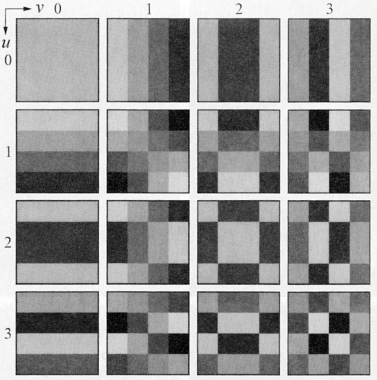
\includegraphics[height=8cm]{figures/dct}
\end{center}
\caption{Discrete-cosine basis functions for $N = 4$. The lighter the color, the larger the value. \cite[p. 473]{Gonzalez2002}}
\label{dctkernels}
\end{figure}
\subsection{Hamming Distance}\label{HammingSection}
According to \cite{Hamming1950} given alphabet $A$ the Hamming Distance $\Delta$ between strings $q \in A$ and $d \in A$ is
\begin{equation}\label{hammingeq}
\Delta(q,d):=\sum_{q_i\neq d_i}1\quad,\quad i=1,\ldots,n
\end{equation}
In other words, it is the number of characters two strings differ. In binary strings it is the number of bits by which two binary numbers differ. Table \ref{hammingexamples} provides some examples. The Hamming Distance can be used to for content based image retrieval by comparing the incoming image hash and the hashes in the database by eq. \ref{hammingeq}. If the Hamming Distance is within some threshold, the image can be said to be in the database.

\begin{table}[htb]
\caption{Hamming Distance for strings.}
\label{hammingexamples}
\begin{center}
  \begin{tabular}{ccr}
&&$\Delta(q,d)$\\
    \hline \hline
    101 & 111 & 1\\
    \hline
    123 & 321 & 2\\
    \hline
    foo & bar & 3\\
    \hline
\end{tabular}
\end{center}\end{table}

\clearpage
\section{Large-Scale Image Retrieval}
Local Features are a good candidate for replacing the perceptual hashes. Image descriptors based on local features are by definition invariant to isotropic scaling and rotation and can withstand some affine distortion, noise and illumination changes.

To compare the perceptual hash based detectors to the Local Features based detector, we simulate near-duplicate cases on two image datasets, the Paintings dataset and the ThingLink dataset. The performance of each classifier is then compared head-to-head. Perceptual hashing is a good choice for implementing near-duplicate image detection due to simplicity of implementation and the ability to scale the solution to millions of images. The trade-off will be complexity of implementation vs. improvement in the results.

We will review state-of-the-art in large-scale image retrieval and it's use for near duplicate image detection. We will find out if in theory, is it feasible to deploy Local Features at a scale of 5 million images at ThingLink for improved near-duplicate detection?
\subsection{Detection and Description of Local Features}
 With hashing, the image identifier is created from the image pixels to form a binary string of fixed length. We expect the Local Features-based NDID system to improve over perceptual hashing as the hashes are unstable image transformations that alter the relationships between spatial pixel values such as rotation and adding and removing from the image.

Instead taking pixel values directly as input, Local Features form an image descriptor by finding large amount of scale-, illumination-, noise- and affine distortion invariant keypoints. Synonyms for Local Features are many in literature. David Lowe used \emph{keypoint} in \cite{Lowe2004}, a seminal work in the field. In describing \emph{Speeded Up Robust Features}, \emph{interest points} is used. Sivic and Zisserman refer to \emph{viewpoint invariant regions}. In this paper we will use \emph{local features} and the short version \emph{feature}. \emph{Feature} detectors and descriptors have been widely developed during the past decade. Object- or scene retrieval, or in our case, near-duplicate image retrieval using local features generally takes the following steps:
\clearpage
\begin{enumerate}
\item Find features of interest in image
\item Encode features in a visual descriptor stored in memory or disk
\item Find nearest neighbors for query descriptor among all known descriptors.
\end{enumerate}

Local Features were invented when Moravec \cite{Moravec1981} from the Stanford AI Lab invented the corner detector in the early 1980s. The Moravec corner detector was improved by Harris and Stephens \cite{Harris1988} by using a Gaussian window function instead of the binary window used by Moravec. The Harris detector was not scale invariant, which lead David Lowe to come up with the \emph{Scale Invariant Feature Transform} (SIFT). SIFT has inspired many similar methods including Speeded Up Robust Features (SURF), BRISK and ORB not covered in this paper. We will however cover KAZE, and AKAZE features, more recent methods using local features.

\subsubsection{Scale Invariant Feature Transform} \label{SIFTSection}
According to David Lowe in \cite{Lowe2004}, the Scale Invariant Feature Transform (SIFT) ''transforms image data into scale-invariant coordinates relative to local features''. SIFT-descriptors are suitable for matching images of the same object or scene. They are robust to image scaling, rotation and somewhat robust to change in viewpoint, scene lighting and affine distortion. Descriptors can be computed on ''off the shelf''-hardware in near real time. A SIFT-descriptor has a location $t_x, t_y$ a scale $s$ and rotation $\theta$. A SIFT-descriptor is the vector $(s, \theta, t_x, t_y)$. SIFT features are visualized in fig. \ref{siftfeatures}. SIFT descriptors are extracted by

\begin{enumerate}
\item Scale space extrema detection identifies scales and locations that can be repeatedly extracted under changing conditions
\item Keypoint localization
\item Orientation assignment
\item Keypoint descriptor.
\end{enumerate}

\begin{figure}[htb]
\begin{center}
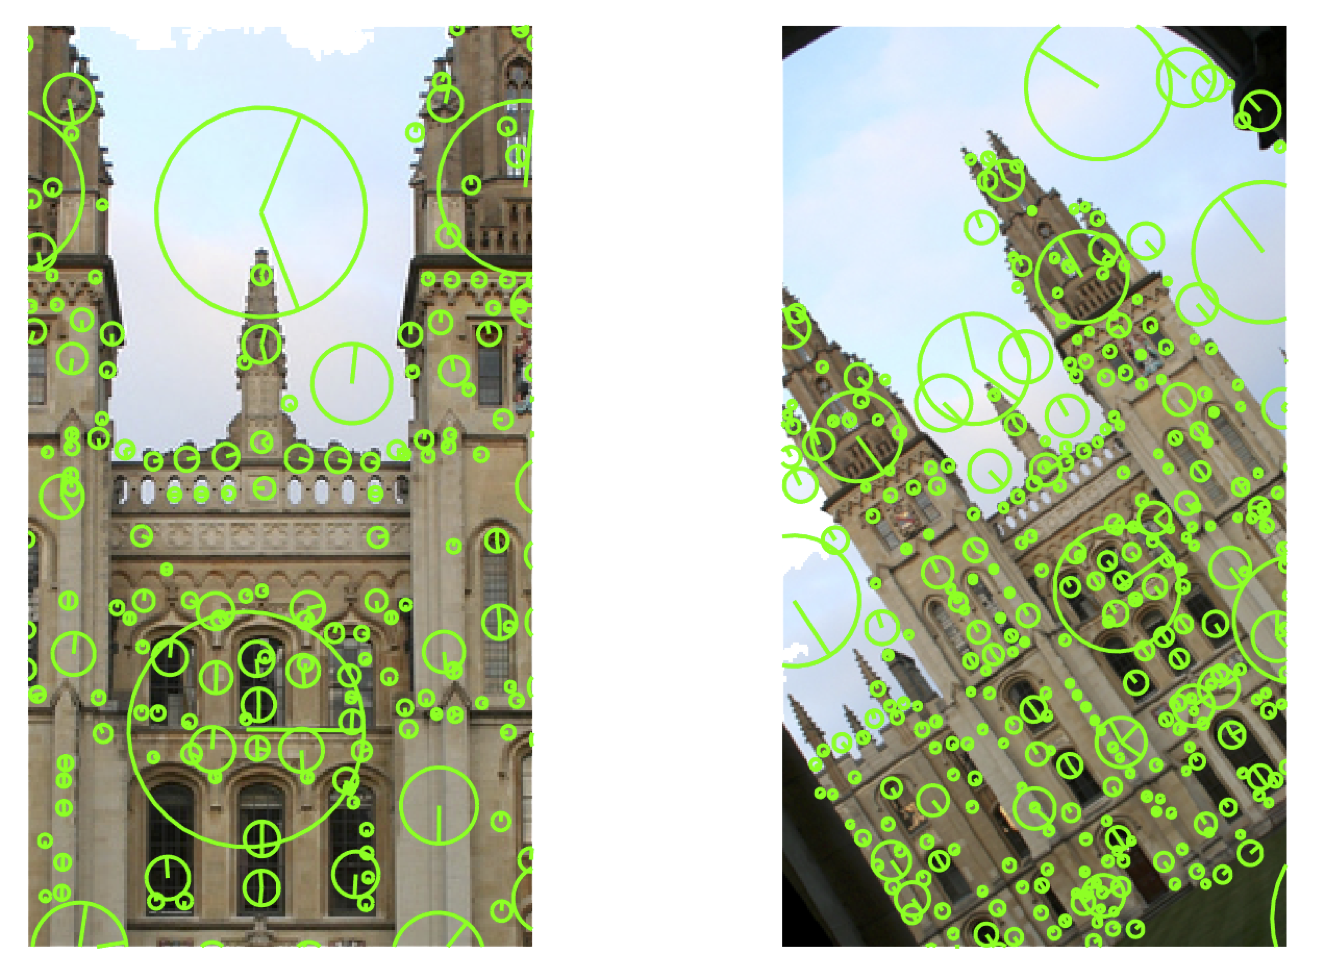
\includegraphics[height=8cm]{figures/siftDescriptor}
\end{center}
\caption{SIFT-descriptors visualized in two images of the same scene.}
\label{siftfeatures}
\end{figure}
To find scale space extrema $D$, a difference-of-Gaussian function is convolved with $I$.
\begin{equation}\label{keypoints}
  D(x,y,\sigma) = (G(x,y,k\sigma) - G(x, y, \sigma))*I(x,y)
\end{equation}
where $G(x,y,k\sigma) - G(x, y, \sigma)$ may be approximated by a normalized Laplacian so
\begin{equation}\label{approximatedog}
G(x,y,k\sigma) - G(x, y, \sigma) \approx (k - 1)\sigma^{2}\nabla^{2}G
\end{equation}
where the right hand side is a scale-normalized Laplacian of Gaussian. $D$ are keypoint candidates. The robust keypoints are weeded out by fitting them to the surrounding data. \cite{Lowe2004}

\clearpage

\begin{equation}\label{keypointoffset}
\hat{\boldsymbol{x}} = - \frac{\partial^2D^-1}{\partial \boldsymbol{x}^2}\frac{\partial D}{\partial \boldsymbol{x}}
\end{equation}
Adding the offset (eq. \ref{keypointoffset}) to $\boldsymbol{X}$. If $\boldsymbol{\hat{x}} > 0.5$, the extremum is closer to another interest point.
\begin{equation}\label{rejectkeypoint}
D(\boldsymbol{\hat{x}})= D + \frac{1}{2}\frac{\partial D^T}{\partial \boldsymbol{x}}\boldsymbol{\hat{x}}
\end{equation}
is used for quality control and any point where $D(\boldsymbol{\hat{x}})<0.03$ they can be discarded. Additional quality control, which we will not cover here takes place. In order to promote rotation invariance, the keypoint is assigned an orientation. Orientation is assigned by calculating gradient orientation $\theta(x,y)$ (eq. \ref{gradientorient}) and magnitude $m(x,y)$ (eq. \ref{gradientmag}) 360 degrees around the keypoint in 36 bins. The orientation will be in the direction of the bin with the greatest magnitude. \cite{Lowe2004}
\begin{equation}\label{gradientmag}
\sqrt{(L(x+1,y)-L(x-1,t))^2 + (L(x, y+1)- L(x, y-1))^2}
\end{equation}
\begin{equation}\label{gradientorient}
\theta(x,y) = tan^{-1}((L(x, y+1)- L(x,y-1))/ (L(x+1,y)-L(x-1,y))
\end{equation}
The SIFT-descriptor is a 128 dimensional vector formed according to figure \ref{siftdescriptor}. It encodes gradient magnitude and direction for 16 bins 8 gradients each.
\begin{figure}[htb]
\begin{center}
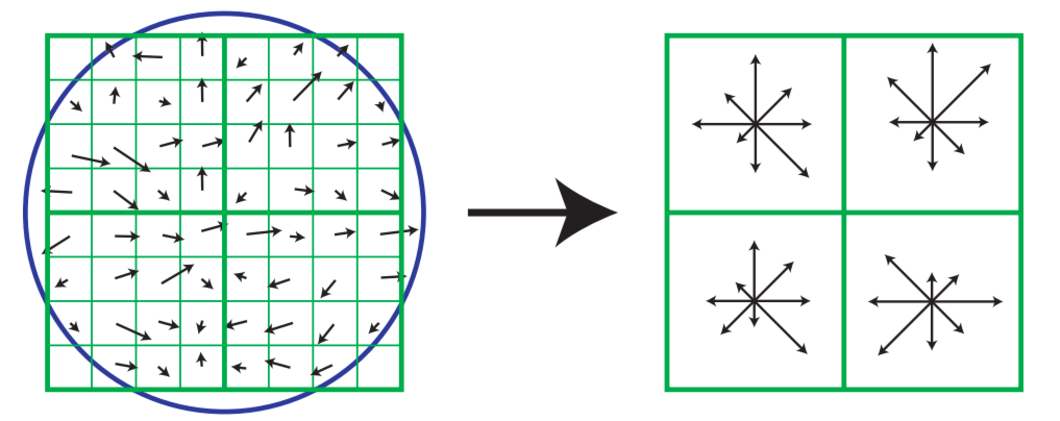
\includegraphics[height=6cm]{figures/siftDescriptorFormat}
\end{center}
\caption{SIFT-descriptor format. A 2 $\times$ 2 example of the descriptor. Best results come from a 128 dimensional descriptor. It is formed from 4 $\times$ 4 subregions each with 8 gradients. \cite{Lowe2004}}
\label{siftdescriptor}
\end{figure}
SIFT as demonstrated in \cite{Lowe2004} uses Best-Bin-First (BBF) indexing for finding approximate nearest neighbors for individual descriptors during queries. To find a matching object or scene in the database the query descriptors are matched one by one to a database of all known descriptors. The quality of individual matches is improved by finding clusters of 3 matches that agree on an object or scene. The clusters are then checked by verifying geometric fit to the model (\emph{geometric verification}) rejecting those matches not fitting to the model.

\subsubsection{Speeded Up Robust Features}
Speeded Up Robust Features (SURF) was introduced in \cite{Bay2006} for faster detection of local features and faster computation of the descriptor than state-of-the-art methods of the time. SURF introduces the 'Fast-Hessian' detector that relies on box filter approximations of Gaussian filters and integral images to reduce the computation time by $\frac{2}{3}$ compared to the difference of Gaussians approach taken by SIFT. According to \cite{Viola2001}, an integral image
\begin{equation}
  \label{integralimage}
ii(x,y) = \sum\limits_{x'\le,y'\le y} i(x', y')
\end{equation}
at point $x, y$ sums up the pixels above and below where $i(x,y)$ is the source image.
\begin{equation}
  \label{integralimagerowsum}
s(x,y) = s(x, y - 1) + i(x,y)
\end{equation}
\begin{equation}
  \label{integralimagepartial}
  ii(x,y) = ii(x-1,y) + s(x,y)
\end{equation}
The integral image is very quick to calculate using the cumulative row sum $s(x,y)$ (eq. \ref{integralimagerowsum}) and recurrence (best viewed in figure \ref{integralimagefig}) within integral images (eq. \ref{integralimagepartial}) with $s(x, -1) = 0$ and $ii(-1,y)=0$. A rectangular sum follows from four array references in figure \ref{integralimagefig}.

\begin{figure}[htb]
\begin{center}
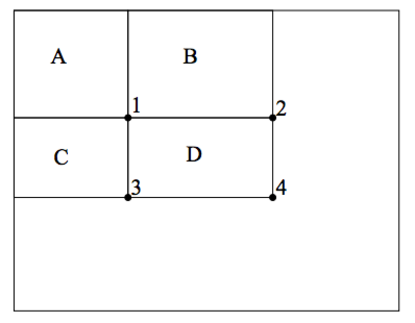
\includegraphics[height=8cm]{figures/integralimage}
\end{center}
\caption{Rectangular sums from integral images. Point 1 is the sum of pixels in A. Point 4 is $A + B + C + D$.\cite{Viola2001}}
\label{integralimagefig}
\end{figure}
According to \cite{Bay2006}, the calculation of the descriptor also uses integral images for speed. The descriptor is a distribution of Haar-wavelet responses in the neighborhood of the interest point. The orientation of the descriptor is determined by Haar-wavelet responses in $x$ and $y$ directions in the scale $s$ that the keypoint was detected with $6s$ radius at sampling step size also $s$. Wavelet size is $4s$. Responses are weighted with a Gaussian $(\sigma = 2.5s)$ at the interest point. The dominant direction is estimated by summing up the responses over a sliding window angle of $\frac{\pi}{3}$. The sum of the horizontal and vertical results form a new vector and the longest vector angle is the interest point orientation. The SURF descriptor is a square region centered on the interest point. The size of the region is $20s$ and is split into $4 \times 4$ sub-regions. Let $d_x$ and $d_y$ be Haar wavelet responses in along horizontal and vertical region edges respectively. For robustness, the responses are weighted with a Gaussian $(\sigma = 3.3)$ and $d_x, d_y$ are summed independently to form the first part of the sub-region descriptor in eq. \ref{surfdescriptor}.
\begin{equation}
  \label{surfdescriptor}
v = (\sum d_x, \sum d_y, \sum \abs{d_x}, \sum \abs{d_y})
  \end{equation}
The second part of the descriptor, $\sum \abs{d_x}, \sum \abs{d_y}$ accounts for sizes of polarity changes. As each region is represented by $4 \times 4$ sub-regions, each region generates a 64 length descriptor. Normalization to a unit vector provides scale invariance while the wavelet responses are invariant to luminance changes.

Queries are performed by matching query image descriptor database image descriptors individually. A match is found if the second nearest neighbor is closer than 0.7 $\times$ NN. In other words, SURF uses the nearest neighbour ratio matching strategy. Geometric verification reduces false positive count (FP). Matching requires fast indexing and additionally storing the sign of the Laplacian for the interest point speeds up searches. The 'Fast-Hessian' detector in the SURF paper was found to be three times faster than the DoG detector by Lowe used in SIFT. SURF improved over SIFT in recall by $4.5\%$. \cite{Bay2006}

\subsubsection{KAZE Features}
A more recent feature detection and description method introduced Alcantarilla et. al in \cite{Alcantarilla2012} improves especially on the difference of Gaussians detection method of SIFT. The name KAZE, Japanese for wind, is a tribute to Iijima, inventor of scale space analysis. KAZE improves SIFT with nonlinear diffusion filtering in place of the difference of Gaussians scale space for detecting relevant features. Nonlinear diffusion filtering maintains or enhances edges \cite{Weickert1998}. There is no down-sampling of the scale space like in SIFT. The computation time is similar to SIFT but slower than SURF. KAZE especially improves $\mathcal{R}$ over SIFT and SURF sometimes improving by 40\%. Gaussian blurring in Gaussian scale space blurs detail and noise alike. Nonlinear diffusion filtering by Additive Operator Scaling however builds the scale space in a way which that reduces noise and leaves object boundaries unblurred leading to improved localization accuracy and distinctiveness. Computation time is comparable to SIFT and slower than SURF. For KAZE features one must
\begin{enumerate}
\item build nonlinear scale space with Additive Operator Splitting
\item detect interesting 2D features via maxima of a scale-normalized determinant of Hessian response through the nonlinear scale space
\item compute M-SURF descriptor orientation and scale from first order image derivatives.
\end{enumerate}
According to \cite{Alcantarilla2013} nonlinear diffusion (eq. \ref{nonlineareq}) where $L$ is the luminance, $c$ is the conductivity function and by choosing this conductivity function in a good way the diffusion will adapt to the image structure $x, y$ and is dependent also on time $t$, which is the scale parameter. According to  \cite{Alcantarilla2012} as $t$ grows, the filtered image is simplified.
\begin{equation}
  \label{nonlineareq}
  \frac{\partial L}{\partial t} = \nabla \cdot c(x,y,t)\cdot\nabla L
\end{equation}

The conductivity function (eq. \ref{conductivityfunceq}) has the image gradient magnitude controlling the diffusion
\begin{equation}
  \label{conductivityfunceq}
c(x,y,t)=g(\abs{\nabla L_\sigma(x,y,t)})
\end{equation}
Perona and Malik covered several conductivity functions in \cite{Perona1990} and we will focus on $g_2$ (eq. \ref{gtwoeq}) which creates the best overall classifiers according to data in \cite{Alcantarilla2012}. $\lambda$ is a contrast factor and parametrizes the level of diffusion where $\nabla L_{\sigma}$ is the gradient of the source image convolved with a Gaussian.
\begin{equation}
  \label{gtwoeq}
g_2 = \frac{1}{1 + \frac{\abs{\nabla L_\sigma}^{2}}{\lambda^{2}}}
\end{equation}
According to \cite{Weickert1998}, $\nabla L_{\sigma}$ can be regarded as the edge detector where if $\abs{\nabla L_{\sigma}} > \lambda$ an edge has been encountered. If $\abs{\nabla L_{\sigma}} < \lambda$ we are dealing with a region and diffusivity (filtering) is increased. For queries the original KAZE paper \cite{Alcantarilla2012}, like SURF in \cite{Bay2006} employ the nearest neighbor distance ratio. High quality matches between two images are then filtered for outliers.

\subsubsection{Accelerated KAZE Features}
According to \cite{Alcantarilla2012}, the main drawback of KAZE features is the slow nonlinear diffusion filtering used for building the nonlinear scale space.  The KAZE method of choice is Additive Operator Scaling (AOS). AOS requires computationally intensive solving a of large system of linear equations. A-KAZE features also introduced by Alcantarilla et. al in \cite{Alcantarilla2013} solves this problem by replacing AOS with Fast Explicit Diffusion (FED) reducing computation time of the nonlinear scale space. In addition, AKAZE uses a Modified-Local Difference Binary (M-LDB) descriptor over M-SURF descriptor used in KAZE.

Fast Explicit Diffusion (FED) introduced in \cite{Grewenig2010} is able to build the nonlinear scale space faster than AOS. AKAZE improves in speed over KAZE, SURF, and SIFT. FED is equivalent to box filtering and can provide good quality approximations of Gaussian kernels and is easy and fast to implement. The factorization of the box filter
\begin{equation}
  \label{boxfilterfactor}
\tau_j = \frac{\tau_{max}}{2cos^2\left( \pi \frac{2j+1}{4n+2}\right)}
\end{equation}
where $n$ is the number of explicit diffusion steps, $\tau_{max}$ is the maximum step size keeping the stability condition of the explicit scheme intact. The FED cycle stopping time $\theta_n$
\begin{equation}
\theta_n = \sum_{j=0}^{n-1}\tau_j=\tau_{max}\frac{n^2+n}{3}
\end{equation}
Equation \ref{nonlineareq} can be discretized as
\begin{equation}
  \label{discretenonlineareq}
\frac{L^{i+1}-L^i}{\tau}=A(L^i)L^i
\end{equation}
where
\begin{equation}
  \label{fednextevolution}
  L^{i+1}=(I + \tau A(L^i))L^i
\end{equation}
$A(L_i)$ is the image conductivity matrix and $\tau$ is the constant step size on condition $\tau < \tau_{max}$ to meet stability conditions. FED cycles while building the scale space are run from short to long. A scale space consists of $O$ octaves (index $o$) and $S$ (index $s$) sub-levels. Scale $\sigma$ is
\begin{equation}
  \label{scalespace}
  \sigma_i(o,s) = 2^{o+s/S},o \in[0\ldots O-1], s \in [0\ldots S-1], i \in [0 \ldots M]
  \end{equation}
where the number of filtered images is $M$.
\begin{equation}
  \label{scaletotime}
t_i = \frac{1}{2}\sigma^2_i,\{i=0\ldots M\}
\end{equation}
\clearpage
To reduce noise the source image may be processed with a Gaussian of $\sigma_0$. The contrast factor $\lambda$ is the 70th percentile of the input image gradient histogram. The pyramidal FED scheme consists of an outer-  and an inner loop. The inner loop performs the filtering according to step sizes set by the outer loop. The outer loop also takes care of down-sampling with mask $(\frac{1}{4}, \frac{1}{2}, \frac{1}{4})$. The down-sampled image is the input to the next octave. For 2D images the maximum step size is $\tau_{max}$ when the image derivative grid size is 1px. The contrast parameter $\lambda$ also needs to be modified for each octave as the down-sampling mask reduces contrast by 25\%. A Hessian (eq. \ref{akazehessian}) is calculated for each $L^i$
\begin{equation}
  \label{akazehessian}
L^i_{Hessian} = \sigma^2_{i,norm}(L^i_{xx}L^i_{yy}-L^i_{xy}L^i_{xy})
\end{equation}
to obtain features. Scharr filters with step size $\sigma_{i,norm}$ are used to compute the second order derivatives. In order to be accepted as a feature location, a maxima has to
\begin{enumerate}
\item in a $3 \times 3$ window where it has to be a maxima
\item it has to be greater than a threshold
\item it is maxima at level $i+1$ and $i-1$ in a $\sigma_i\times\sigma_i$ window
\end{enumerate}

As described in \cite{Alcantarilla2012}, after detection the precise interest point location is found by finding best fit of a quadratic function to the Hessian response determinant in the $3 \times 3$px neighborhood and finding the maximum. A-KAZE uses a Modified Local Difference Binary descriptor. The LDB descriptor is modified to speed up calculations relating to rotation invariance. LDB stores intensity, means of the horizontal and vertical derivatives. LDB uses grids of finer steps dividing the descriptor into sub-grids. M-LDB rotates these LDB grids to the interest point orientation. Due to this rotation, integral images may not be used to calculate averages of pixels inside the sub-grids, the sub-grids are sub-sampled in steps which are a function of the scale $\sigma$ M-LDB re-uses the derivatives from the detection step in the descriptor. Descriptor distance to another descriptor may be determined via $\Delta(q,d)$ not unlike calculating distance in perceptual hashing.

\clearpage

\subsection{Retrieval}
ThingLink hosts 5 Million annotated scenes. Large-Scale Image Retrieval is an umbrella term for using an image to query for object-, scene-, category-, or duplicate among millions of images. In \cite{Wang2013} Wang et. al query near-duplicates among billions of images. However, their approach used batch processing. We are interested in a smaller scale and preferably near realtime implementations. Some of the more important limitations with the near realtime case have to do with fitting the database into main memory for a OTS hardware. When all the descriptors in the database do not fit into system RAM, the efficiency of the retrieval system collapses due to disk access \cite{Philbin2007}. In order to match among numerous of images, the descriptors are quantized into visual words to speed up the search. In order to further optimize search \cite{Jegou2010} optimizes the descriptor format for memory footprint optimization and computation speed.

Detection and description of features covered finding interesting points in an object or scene and creating a serialization, an image descriptor to add to the database of all known images. This section covers efficient querying in that database possibly consisting of millions of images.

Finding an image duplicate is a special simplified case where the highest result is assumed to contain the duplicate. The first step after calculating the descriptor for a query image is finding the nearest neighbors for each descriptor in the database. The SIFT descriptor is usually 128 dimensional, which makes the NN-search especially challenging.

\subsubsection{Nearest Neighbor Search}
Matching a new image descriptor to a set of known image descriptors can be as simple as a Euclidean nearest neighbor search (eq. \ref{nneq}) which Donald Knuth also named as the \emph{post-office problem} in vol. 3 of The Art of Computer Programming (1973). It answers the question ''To which post office does this address belong to?'' which is analogous to ''which known image descriptor is closest to this new image descriptor?''.

Matching in a set of millions of images is not feasible in user facing applications as the time complexity is $\mathcal{O}(nd)$ where $n$ is the number of image descriptors in the set and $d$ is the dimensionality of each image descriptor.


\begin{equation}
\label{nneq}
NN(x) = arg \min_{y\in Y}\norm{x-y}^2
\end{equation}

\begin{figure}[htb]
\begin{center}
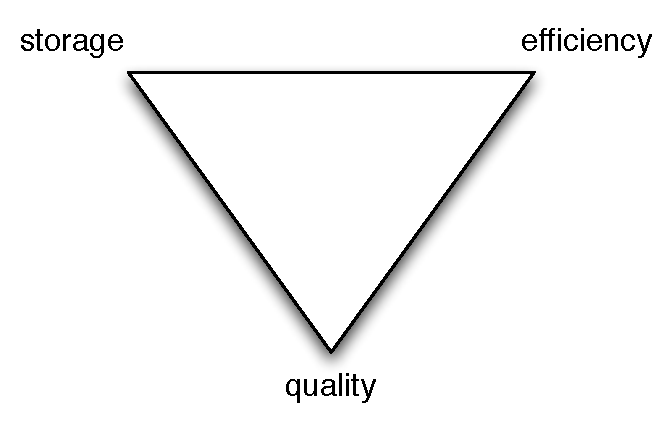
\includegraphics[height=4cm]{figures/nntradeoffs}
\end{center}
\caption{Tradeoffs for improving nearest neighbor search}
\label{nntradeoffs}
\end{figure} To improve scalability, one can relax the conditions on nearest neighbor. The tradeoffs involved (fig. \ref{nntradeoffs}) are memory footprint, as the descriptors the faster the memory the descriptors are stored in, the more computationally feasible matching becomes at large scale. Increasing the quality of the matches will require sacrifices in speed and the memory footprint. Approximate nearest neighbor methods in \cite{Gionis1999} are able to solve the ''curse of dimensionality'' in many cases. Approximate nearest neighbor is defined as in a normed space $l_p^d$ preprocess set of points $P$ to return a point $p\in P$ for query point $q$ holding $d(q,p) \lq (1 + \epsilon)d(q,P)$. The distance from the closest point in $P$ to $q$ is $d(q, P)$.

\subsubsection{Locality Sensitive Hashing}
The original SIFT descriptor has 128 dimensions. The SURF descriptor has 64 dimensions. Since the Nearest Neighbor search (eq. \ref{nneq}) time complexity is dependent on the descriptor dimension $d$, a search in 5 million images scales linearly (poorly). Locality Sensitive Hashing was developed to solve this ''curse of dimensionality'', where $d > 3$ for NN search \cite{Gionis1999}. LSH scales well for $d > 50$ \cite{Gionis1999}. We will only cover the main idea behind the LSH family of methods. A review of the state of the art in 2008 can be found in \cite{Andoni2008}. Finding optimal hash functions for LSH applications has attracted much more recently so we examine \emph{Optimal LSH for Angular Distance} \cite{Andoni2015} by Andoni et al. from 2015.

For hash function $g$ to be Locality-Sensitive, the collision probability increases for points that are nearby versus those that are far away. Hash function quality can be described by $p_1$, the collision probability for points close to each other and $p_2$ the collision probability for distant points.\cite{Andoni2015} Naturally difference between $p_1$ and $p_2$ characterizes hash function reactivity to changes in distance better described by $\rho$ (eq. \ref{lshsensitivity}).
\begin{equation}
  \label{lshsensitivity}
  \rho = \frac{log\frac{1}{p_1}}{log\frac{1}{p_2}}
  \end{equation}
The goal of LSH is to hash data points in a way so the collision probability is high for points close to one another compared to points that are far apart. By allowing for small error (eq. \ref{lsherroreq}) in the results and adding to storage requirements, the query time is significantly improved, giving up quality for speed as seen in fig. \ref{nntradeoffs}. \cite{Gionis1999} The solution presented in \cite{Gionis1999} reduces ANN time complexity to $\mathcal{O}(dn^{\frac{1}{1+\epsilon}})$.

LSH has $m$ hash functions, hash tables and keys per vector. Each point in the set $P$ has $m$ hash keys as an index. At query time $m$ keys are computed on the query vector and all the vectors associated with the new keys are retrieved forming a shorter list where it's feasible to use exact distance for matching. For the Approximate 1-NNS problem the effective error $E$ is
\begin{equation}
  \label{lsherroreq}
E = \frac{1}{\abs{Q}}\sum_{q\in Q}\frac{d_{LSH}}{d^*}
  \end{equation}
where the distance $d^*$ from $q$ to the nearest point over all successful queries. min-Hash is LSH for sets and was originally developed to find similar text documents.

\subsubsection{min-Hash}
min-Hash was used in \cite{Broder1997} to search for similar text documents among 30 million documents. In \cite{Chum2008} upon which this section is based, the same idea is harnessed to find duplicate images for sample data sets. Chum et. al \cite{Chum2010} use min-Hash techniques to find duplicates in $10^4, 10^5$ and $5 \times 10^6$ images. It finds similar images with a probability near to one, near similar images with small probability and unrelated images with 0 probability.

In essence min-Hashing is LSH for sets. Like in the case of perceptual hashes (section \ref{perceptualhash}), two images are considered alike if the result of some similarity function $sim_s$ is higher than some threshold. min-Hashing quantizes and compresses SIFT descriptors. It is included in the retrieval section, as the major contributions lie in the retrieval step for finding near-duplicate objects. It solves issues of storage and efficiency in a proven way for moderately large data sets. The corner stone is min-Hash ability to estimate document or image similarity based on a set of data significantly compressed from the original data set. Considering the 128 dimensional SIFT descriptor and 10 million images, if one uses 400 independent hash functions $f_j:\mathcal{V} \rightarrow R$, $f_j, i = 1 \ldots 400$, the similarities are evaluated on a data set with 128 columns but only 400 rows.

min-Hash (eq. \ref{minhash}) is the smallest element of set $\mathcal{A_i}$ under ordering by $f_j$
\begin{equation}\label{minhash}
m(\mathcal{A}_i,f_j)= arg \min_{X \in \mathcal{A}_i}f_j(X)
\end{equation}
It estimates object (text or image) similarity based on (eq. \ref{minhash}) the probability (eq. \ref{minhashsim}) that sets $\mathcal{A}_1$ and $\mathcal{A}_2$ have equal min-Hashes is the same as their similarity (eq. \ref{similarityminhash}). The used similarity function can vary. Set similarity or Jaccard is similarity demonstrated in eq. \ref{similarityminhash}
\begin{equation}\label{similarityminhash}
sim_W(\mathcal{A}_1,\mathcal{A}_2) = \frac{\abs{\mathcal{A}_1 \cap \mathcal{A}_2}}{\abs{\mathcal{A}_1 \cup \mathcal{A}_2}}
\end{equation}
 and for images drawing inspiration from the \emph{tf-idf} scheme a histogram intersection approach
\begin{equation}\label{similarityminhashimages}
sim_h(\mathcal{A}_1, \mathcal(A)_2)=\frac{\sum_W min(t^w_1,t^w_2)}{\sum_W max(t^w_1,t^w_2)}
\end{equation}
where $t_i$ is size $\abs{\mathcal{V}}$ and $t_i^w$ of the $i$-th document is the count of visual word $X_w$ in that document. $d_w \geq 0$ is the importance of $X_w$. This similarity measure performed better in efficiency and quality than Jaccard distance for the TrecVid 2006 data set.
\begin{equation}\label{minhashsim}
P(m(\mathcal{A}_1,f_j) = m(\mathcal{A}_2,f_j)) = \frac{\abs{\mathcal{A}_1 \cap \mathcal{A}_2}}{\abs{\mathcal{A}_1 \cup \mathcal{A}_2}} = sim_s(\mathcal{A}_1, \mathcal{A}_2)
\end{equation}
Just as a set of words was used in \cite{Broder1997}, to borrow the BoW approach from section \ref{BOW}, an image can be represented as a set of visual words and the min-Hash can be applied to NDID. More specifically, with vocabulary $\mathcal{V}$, an image is represented by a vector of length $\abs{\mathcal{V}}$ containing the number of features falling on a given visual word. To ease retrieval the min-Hashes are organized into \emph{sketches} like in \cite{Broder1997}
\begin{equation}\label{sketch}
(m(\mathcal{A_1},f_1) \ldots m(\mathcal{A_1},f_n))
\end{equation}
which have similarity
\begin{equation}\label{sketchsim}
sim_s(\mathcal{A}_1, \mathcal{A}_2)^n
\end{equation}
Sketching reduces the number of false positives retrieved by min-Hash. The sketch similarity is evaluated first, and only if it is above some threshold the full similarity $sim_s(\mathcal{A}_1, \mathcal{A}_2)$ is evaluated. The probability $P(\mathcal{A}_1 \sim^h \mathcal{A}_2)$ of sets $\mathcal{A}_1$ and $\mathcal{A}_2$ having at least $h$ identical sketches from $k$ picked
\begin{equation} \label{sketchsimilarityprob}
P(\mathcal{A}_1 \sim^h \mathcal{A}_2) = \sum_{i=h}^k \binom{k}{i} p^{in}(1-p^n)^{k-i}
\end{equation}
\cite{Chum2008} modifies the similarity measure with ideas borrowed from \emph{tf-idf} weighting like in \cite{Sivic2003}. This is done by including occurrences of visual words in the representative set for the image in question as a unique member of the set resulting in an \emph{idf} like method \cite{Chum2010}. In the TrecVid 2006 data set, and University of Kentucky database cases it distanced dissimilar documents further apart when common visual words have low \emph{idf} and are weighted down as a result leading to a lower number of sketch hits and better quality search results \cite{Chum2008}. However, \cite{Chum2008} leaves min-hash performance for very large image databases (millions of images) for further research.

Querying large sets of images is considered in \cite{Chum2010} where min-Hash is used for fast detection of duplicate images. This is done by using min-Hash for detection of random pairs of spatially overlapping images. These are named cluster seeds which become queries to find similar images including the seed. In other words
\begin{enumerate}
\item store descriptors in a hash table where the probability of an image being in the same bin is the same as their similarity
\item calculate exact similarity for images falling into the same bin
\item if pair of images pass the similarity test, check spatial consistency
\item if image pair passes step 3., they become cluster seeds.
\end{enumerate}
Their requirements are similar to what is attempted in this paper.
\begin{enumerate}
\item scalable to tens of millions of images
\item adding images to the database does not result in recomputing the entire cluster
\item easy to parallellize
\item probability of recall is independent of cluster size
\end{enumerate}
For querying the Oxford Landmark data set, the seed generation and seed growing steps to find a match took 0.014s per image on a single 2.4GHz core for 100k images. For 5M images clustering took 0.02s per image on a 3GHz single core PC. Growing the data set size in a min-Hash database takes $\mathcal{O}(NL)$ where $N$ is the data set size and $L$ to be the number of images in the cluster. The seed generation is $\mathcal{O}(N^2)$ for infinite size databases but is linear for $N \leq M$ where $M$ is the number of bins in the hashing table. \cite{Chum2010}

In \cite{Lee2010} a high $FP$-rate is a serious problem for large data set. Another problem according to \cite{Chum2010} for direct image retrieval is low recall.

\subsubsection{Bag-of-Visual Words}\label{BOW}
The Bag-of-Visual Words approach to describing images was developed by Sivic and Zisserman in \cite{Sivic2003} by mimicking the approach of text searches into text documents. This is an approach not unlike the Google search engine. Their results show that there is no penalty from using search by visual words vs. n-nearest neighbor methods. To calculate image descriptors two types of viewpoint covariant regions are formed. The first stage iteratively finds an elliptical region around an interest point. The result is an ellipse with a center, shape and scale. Scale comes from a local extremum of a Laplacian. The shape comes from maximizing intensity gradient isotropy over the elliptical region. This is achieved using Shape Adapted (SA) regions.

The second type of region used is the Maximally Stable (MS) region. For these regions are the region area stays constant as the intensity threshold is changed. The two types of regions complement each other in image detection. The SA regions perform well on corners and the MS regions perform well on high contrast blobs. \cite{Sivic2003} The original BoW approach uses SIFT-descriptors introduced by Lowe. The second type of region is implemented in affine covariant regions.

BoW relies on quantizing descriptors into visual words for efficient retrieval. Descriptors are quantized by associating them with the nearest cluster of descriptors. The vector quantization is implemented by k-means clustering. The original BoW implementation worked on video, but we will apply the simple image case only. In the original implementation, the Mahalanobis distance is used as the distance function in k-means clustering. \cite{Sivic2003}

In text retrieval a document is stored in a vector of word frequencies. A weight is usually applied to the vector. Term frequency-inverse document frequency, $tf-idf$ (eq. \ref{tfidf}) is a weighting scheme common in text retrieval. In $k$ words, each document is represented by a $k$-vector $V_{d}=(t_{1},...,t_{k})^{T}$

\begin{equation}\label{tfidf}
t_{i} = \frac{n_{id}}{n_{d}}log\frac{N}{n_{i}}
\end{equation}
with $n_{id}$ is word $i$ appearing $n$ times in document $d$ and $n_{d}$ is the total number of words in document $d$. $n_{i}$ is the total number of occurrences of term $i$. $N$ is the total number of documents. The first term is word frequency and the second term is inverse document frequency. Word frequency weighs words occurring often in a document while inverse document frequency down weights words that appear often in all documents. This weighting scheme outperformed the binary and $tf$ weighting schemes

\begin{equation}\label{bowrank}
  Rank = \frac{1}{NN_{rel}}\left(\sum{i=1}{N_{rel}}R_{i}-\frac{N_{rel}(N_{rel} + 1)}{2}\right)
\end{equation}
where $N_{rel}$ is the number of relevant images for particular query image, $N$ is the total number of images and $R_{i}$ is the $i$th image rank. $Rank$ is a number between 0 and 1. \cite{Sivic2003}

Retrieval uses an inverted file where each word has a hit list for all occurrences of the word in all documents. In the visual word case, each visual word has knowledge of the images it is found in. The document vector is sparse and the retrieval is very fast.

The user specifies an area of interest in a frame and descriptors are calculated for stable regions. The descriptors are then quantized into visual words. A stop list filters out all visual words which occur frequently. Sivic and Zisserman found their case to work best dropping top 5\% and bottom 10\% of words.

Google gives additional weight to words in the search that appear close together in the retrieved document. With visual words, the retrieval is done per frame (image) only and the results are re-ranked based on spatial consistency.

A loose definition would be to require neighboring matches in query image to lie close together also in the retrieved frame.

\subsubsection{Product Quantization} \label{PQ}
Product quantization allows for the packing of image descriptors so they are able to fit in memory of off-the-shelf hardware. More specifically
\begin{equation}
  \label{quantizereq}
d(x,y)^2 \approx d(x,q(y))^2
\end{equation}
where $x$ is the query vector, $y$ is the database vector and quantizer function is $q(y)$. The error on estimated distance is bound by the quantization error, $e_d \leq e_q$.  \cite{Jegou2014}

The quantizer should be fast enough and precise. The database vector $y$ is split $y \rightarrow [y_1 \ldots y_m]$ each of which is quantized $[q(y_1)\ldots q(y_m)]$. For example, and eight dimensional vector can be split into four sub-vectors each in two dimensions. In effect were using $8^4$ centroids with a quantization cost equivalent to using eight centroids. Splitting up the query vector make quantization fast. \cite{Jegou2014}

In \emph{asymmetric distance computation} (ADC) in eq. \ref{adceq}, the database vectors $y$ are quantized but the query is not. This achieves lower distance distortion over the quantized query case (fig. \ref{nosdc}) called \emph{symmetric distance computation} (SDC) not covered here. Distance $d(x,y)$ approximation $\tilde{d}(x,y)$

\begin{equation}
  \label{adceq}
  \tilde{d}(x,y)=d(x, q(y))=\sqrt{\sum_jd(u_j(x),q_j(u_j(y)))^2}
\end{equation}

$d(u_j(x),c_{j,i}) : j = 1\ldots m,i=1\ldots k^*$ are computed prior to the query. Since the square root is monotonically increasing it can be left uncalculated as the ranking of database vectors remains the same regardless of the square root\cite{Jegou2011}

\begin{figure}[htb]
\begin{center}
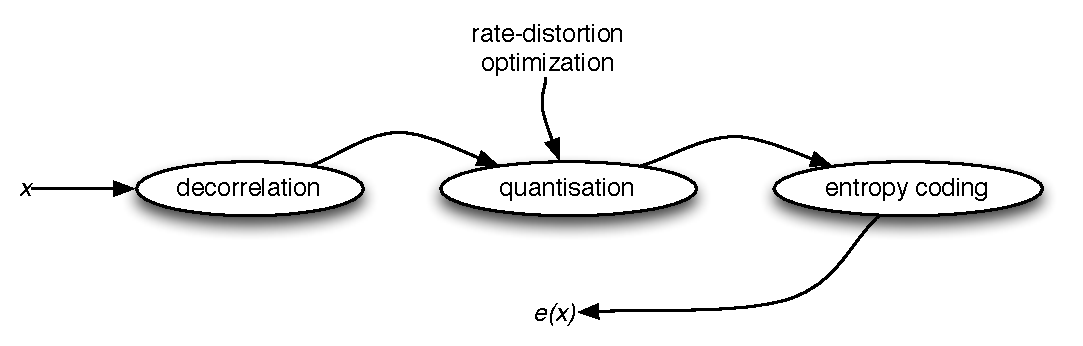
\includegraphics[height=4cm]{figures/pq}
\end{center}
\caption{Simple product quantizer \cite{Jegou2014}}
\label{pqfig}
\end{figure}

\begin{figure}[htb]
\begin{center}
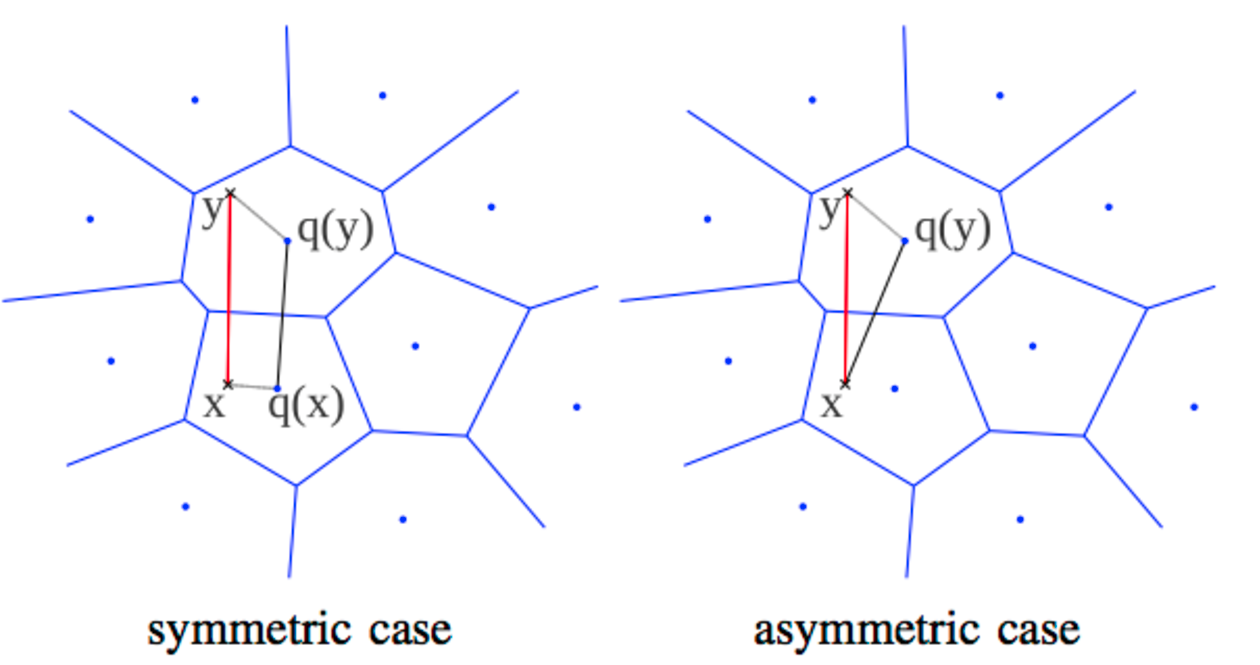
\includegraphics[height=8cm]{figures/sdcadc}
\end{center}
\caption{The increased distance distortion in the symmetric case (SDC) vs. the asymmetric case (ADC) introduced by the extra quantization $q(x)$. \cite{Jegou2008}}
\label{nosdc}
\end{figure}

ANN search with ADC is fast and reduces memory usage with some sacrifice in quality. The search is exhaustive and scales global image description well. If local descriptors are considered, exhaustive search is not feasible due to multiple queries and billions of descriptors \cite{Jegou2008}. In order to make search with local descriptors, the inverted file system from \cite{Sivic2003} is used forming an \emph{inverted file system with asymmetric distance computation} (IVFADC) (fig. \ref{ivfadcfig}).

\begin{figure}[htb]
\begin{center}
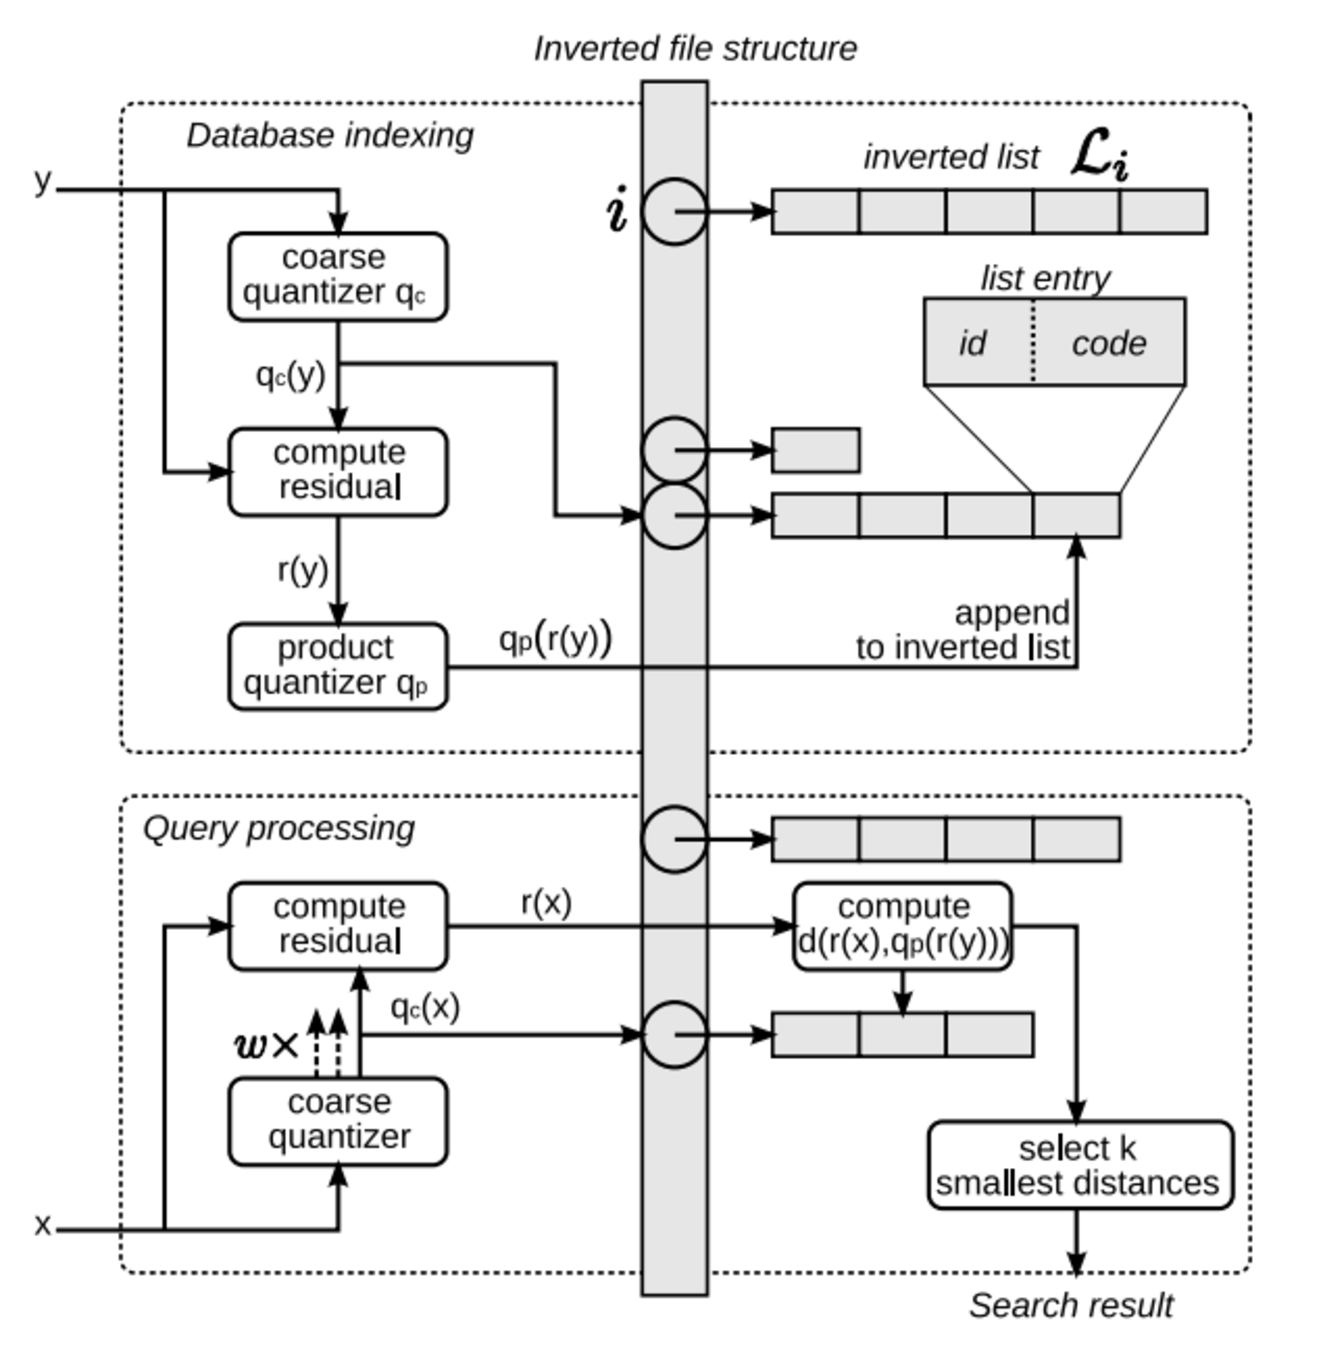
\includegraphics[height=8cm]{figures/ivfadc}
\end{center}
\caption{Block diagram of inverted file with asymmetric distance computation (IVFADC) system. \cite{Jegou2008}}
\label{ivfadcfig}
\end{figure}
The inverted file allows to rapidly access a short list of images close to the query \cite{Jegou2008}. An inverted file entry has and image index and an encoding of the difference between the query vector and the coarse centroid (table \ref{ivfadcentry}).

To set up the inverted file, the coarse quantizer $q_c$ which assigns queries to $\mathcal{L}_i$ is learned using k-means clustering. $1000 \leq k' \leq 1000000$ for SIFT descriptors \cite{Jegou2008}. A product quantizer $q_p$ like in \cite{Sivic2003} is used to encode a residual vector $r(y)$ between the coarse quantized centroid $q_c(y)$ and the vector $y$ (eq. \ref{ivfadcres}). ANN distance $\ddot{d}$ in this scenario where product subquantizers $q_{p_j}$ (eq. \ref{ivfadcestimate}). The distances between $u_j(x-q_c(y))$
and product quantizer $q_{p_j}$ centroids $c_{i,j}$ are computed in advanced and stored in lookup tables. \cite{Jegou2008}

\begin{equation}
  \label{ivfadcres}
r(y) = y - q_c(y)
\end{equation}

\begin{equation}
  \label{ivfadcestimate}
  \ddot{d}(x,y)^2 = \sum_jd\left(u_j(x-q_c(y)), q_{p_j}(u_j(y-q_c(y)))\right)^2
\end{equation}
To add vector $y$ to index $\mathcal{Y}$
\begin{enumerate}
\item calculate $q_c(y)$
\item compute the residual $r(y)$ (eq. \ref{ivfadcres})
\item look up $q_p(r(y))$ by finding $u_j(y)$ per $q_j(u_j(y))$ for all product quantizers ($j = 1 \ldots m$)
\item add new entry (table \ref{ivfadcentry}) to inverted list $\mathcal{L}_i$ in accordance to $q_c(y)$.
\end{enumerate}
When querying $k-ANN(x)$ the inverted list $L_i$ that corresponds to the coarse quantizer result is scanned. It is usual that $x$'s nearest neighbor is not quantized to the same centroid with $x$ but some centroid nearby. $w$ nearest lists $\mathcal{L}_i$ are used instead. According to \cite{Jegou2008}, a k-ANN query of $x$ is performed in the following way:
\begin{enumerate}
\item do $q_c(x)$ to find $w$ nearest lists in $\mathcal{L}_i$ and from subset of $\mathcal{Y}$
\item $\forall j$ do $d(u_j(r(x)), c_{i,j})^2$, the squared distance for sub-quantized values and its centroids
\item sum up $m$ looked up values by executing equation \ref{ivfadcestimate}
  \item select K nearest neighbors of $x$ from subset of $\mathcal{Y}$.
\end{enumerate}
If $\mathcal{L}_i$ are balanced, roughly $n \times \frac{w}{k'}$ entries have to be visited where $k'$ is the number of centroids in $q_c$ and $w$ is the number of NN for $q_c(x)$ retrieved \cite{Jegou2008}.

\def\arraystretch{1.5}
\begin{table}[htb]
\caption{Inverted list $\mathcal{L}_i$ entry with identifier and encoded residual $q_P(r(y))$ \cite{Jegou2008}}
\label{ivfadcentry}
\begin{center}
\begin{tabular}{lc}
  field & length (bits)\\
  \hline
  identifier&8-32\\
  code & $m[\log_2k^*]$\\
\end{tabular}
\end{center}\end{table}

\subsubsection{The Fisher Vector}\label{FV}
The Fisher kernel brings the best of both pattern classification with generative and discriminative methods \cite{Jaakkola1999}. The Fisher kernel transforms a variable-size set of independent samples into a fixed size vector, the Fisher Vector (FV) (eq. \ref{fishervectorfinal}), given samples follow a training set based generative model \cite{Jaakkola1999}. Variable-size accommodates for variable amounts of features extracted from an image. It was applied to image classification by by Perronin et al. \cite{Perronnin2007} and improved in \cite{Perronnin2010} where images are treated as signals and the generative model (GMM) is a kind of visual vocabulary. Perronnin in \cite{Perronnin2010a} extends FV for use in large-scale image retrieval. Similar to $tf-idf$, it discounts the influence of common visual words (Gaussians in this case).

The Fisher vector according to \cite{Perronnin2010} can be used to process local descriptors. $X = {x_t, t = 1 \ldots T}$ is a set of T local feature descriptors of an image generated by a process modeled by $u_\lambda$.
\begin{equation}\label{fishervector}
 G_\lambda^X = \frac{1}{T}\nabla_\lambda\log u_\lambda(X)
\end{equation}
describes $X$ as gradient vector. The dimensionality of $G_\lambda^X$ depends only on the number of parameters in $\lambda$, not on $T$ \cite{Perronnin2010}. As different images have different numbers of interest points, this method allows for images in a database to be represented by codes of equal dimension. Eq. \ref{fishervector} describes the direction in which parameters should be adjusted to best fit the model. One may characterize a signal with a gradient vector derived from a generative probability model $u_\lambda$ and to subsequently feed this representation to a discriminative classifier. \cite{Perronnin2007}

We walk through the formation of the Fisher Vector as done in \cite{Perronnin2010}. The Fisher information matrix of $u_\lambda$ is $F_\lambda$.
\begin{equation}\label{fishermatrix}
F_\lambda = E_{x~u_\lambda}[\nabla_\lambda\log u_\lambda(x)']
\end{equation}
As shown in \cite{Jaakkola1999} a Fisher kernel for $G_\lambda^X$ is
\begin{equation}\label{fisherkernel}
K(X,Y) = G_\lambda^{X'}F_\lambda^{-1}G_\lambda^Y \quad \cite{Perronnin2010}
\end{equation}

As the Fisher information matrix $F_\lambda$ is symmetric and positive definite, a Cholesky decomposition exists as $F_\lambda = L_\lambda'L_\lambda$ $K(X,Y)$ becomes
\begin{equation}\label{fishervectorfinal}
\mathcal{G}_\lambda^X = L_\lambda G_\lambda^X
\end{equation}
also known as the \emph{Fisher vector} of X \cite{Perronnin2010}. $u_\lambda$ is chosen to be a Gaussian mixture model (GMM) (eq. \ref{gmmeq}) where each $u_i$ is analogous to a visual word the size of the vocabulary being $K$ \cite{Perronnin2010a}
\begin{equation}\label{gmmeq}
u_\lambda = \sum_{i=1}^K w_iu_i(x)
\end{equation}
trained by Maximum Likelihood Estimation (MLE) and an image training set. Model parameters $\lambda$ are
\begin{equation}\label{lambdaparams}
\lambda = {w_i,\mu_i, \Sigma_i, i=1 \ldots K}
\end{equation}
where $w_i$ is the mixture weigh, $\mu_i$ is the mean and $\Sigma_i$ is the covariance matrix of Gaussian $u_i$ \cite{Perronnin2010}. $x_t$ are assumed independently generated by the GMM so
\begin{equation}\label{gmm}
G_\lambda^X = \frac{1}{T}\sum_{t=1}^T \nabla_\lambda \log u_\lambda(x_t) \quad \cite{Perronnin2010}
\end{equation}

$\gamma_t(i)$ is a soft assignment of descriptor $x_t$ to Gaussian $i$
\begin{equation} \label{descriptortogaussian}
\gamma_t(i) = \frac{w_iu_i(x_t)}{\sum_{j=1}^Kw_ju_j(x_t)}
\end{equation}
and gradient vector $\mathcal{G_\lambda^X} = [\mathcal{G}_{\mu,i} \mathcal{G}_{\sigma,i}] $ where
\begin{equation}\label{fishervectormu}
\mathcal{G}_{\mu,i}^X = \frac{1}{T\sqrt{w_i}} \sum^T_{t=1} \gamma_t(i)\left(\frac{x_t - \mu_i}{\sigma_i}\right)
\end{equation}
is the gradient with respect to the mean $\mu_i$ and
\begin{equation}\label{fishervectorsigma}
\mathcal{G}_{\sigma,i}^X = \frac{1}{T\sqrt{2w_i}} \sum_{t=1}^T \gamma_t(i)\left[\frac{(x_t - \mu_i)^2}{\sigma_i^2} -1\right]
  \end{equation}
is the gradient with respect to the standard deviation $\sigma_i$ (vector division is done term by term). \cite{Perronnin2010}

The Fisher vector has not been used extensively for large-scale retrieval possibly due to very high dimensional representations (100k even) \cite{Perronnin2010a}. However, when combined with LSH and a binarization technique large-scale retrieval becomes feasible as shown in \cite{Perronnin2010a}.

Estimating the Nearest Neighbor between Fisher Vectors can be performed via dot-product (eq. \ref{fisherdoteq}) \cite{Perronnin2010a}, a simple operation. For the actual implementation in \cite{Perronnin2010a} cosine similarity (dot product of L2-normalized vectors) is used. This guarantees retrieval of the query image first if it is contained in the image database \cite{Perronnin2010a}.

Writing eq. \ref{fishervectormu} in equations \ref{fishernormdistance}, \ref{fishertotalassignment} and \ref{fishermeanassignment} we get
\begin{equation}\label{fisherrewrite}
\frac{1}{T}\mathcal{G}_i^X=\frac{w_i^X}{\sqrt{w_i}}\delta_i^X
\end{equation}
so the dot product of image $X$ and $Y$ Fisher vectors is proportional to
\begin{equation}\label{fisherdoteq}
\mathcal{G}_\lambda^{X'}\mathcal{G}_\lambda^Y \propto \sum_{i=}^N\frac{w_i^Xw_i^Y}{w_i}\delta_i^{X'}\delta_i^Y,
\end{equation}
where
\begin{equation}\label{fishernormdistance}
\delta_i^X = \frac{\mu_i^X - \mu_i}{\sigma_i},
\end{equation}
and for visual word $i$ $w_i^X$ is the fraction of descriptors of image $X$ soft-assigned to it
\begin{equation}\label{fishertotalassignment}
w_i^X = \frac{1}{T}\sum_{t=1}^T\gamma_t(i).
  \end{equation}
$\mu_i^X$ is the mean of $X$s descriptors divided by the probability of assignment to the $i$th Gaussian
\begin{equation}\label{fishermeanassignment}
\mu_i^X=\frac{\sum_{t=1}^T\gamma_t(i)x_t}{\sum_{t=1}^T\gamma_t(i)}.
\end{equation}

The $\frac{w_i^Xw_i^Y}{w_i}$ on the right side of eq. \ref{fisherdoteq} is the product of visual word $i$ frequency in images $X$ and $Y$, the \emph{term frequency} in \emph{tf-idf} divided by the global frequency of i, in other words the \emph{inverse document frequency} analogous to the \emph{idf} implementation in \cite{Sivic2003}.

If $\delta_i^{X'}$ and $\delta_i^{Y}$ have similar direction and a large norm, $\delta_i^{X'}\delta_i^{Y}$ in equation \ref{fisherdoteq} is large. Their direction is similar if the descriptors of $X$ and the descriptors of $Y$ assigned to visual word (Gaussian) $i$ have a similar average. $\delta_i^{X'}$ and $\delta_i^{Y}$ have a large norm if $\mu_i^X$ and $\mu_i^Y$ are far from the Gaussian mean $\mu_i$ of the visual word (Gaussian) of $i$. \cite{Perronnin2010a}

\subsubsection{Vector of Locally Aggregated Descriptors}
Since the introduction of BoW \cite{Sivic2003}, one of the most outstanding contributions in the field of feature detection and description is the \emph{Vector of Locally Aggregated Descriptors} (VLAD) making it possible to store all the descriptors of a very large data set into main memory for fast matching and retrieval \cite{Arandjelovic2013}. The indexing approach in \cite{Sivic2003} and \cite{Jegou2008} using inverted index becomes unfeasible due to search efficiency (speed) and memory consumption of the image descriptors for large scale \cite{Jegou2010}.

VLAD optimizes the three constraints in fig. \ref{nntradeoffs} for NN-search jointly. There are two limits to the number of images that can be indexed in practice. The memory footprint of one image descriptor and the search efficiency. Search efficiency was solved by min-Hashing \cite{Chum2008}, \cite{Chum2009} but they still maintain a significant memory footprint \cite{Jegou2010}.

VLAD was developed in order to represent local descriptors so image searches could be scaled with accuracy, efficiency and low memory consumption drawing inspiration from BoW and the Fisher Vector (FV) (section \ref{FV}). In \cite{Jegou2012} VLAD is shown to be a non-probabilistic FV. VLAD greatly exceeds BoW in performance for a set of images of the same size. It provides good search accuracy with reasonable vector dimensionality. It jointly optimizes reduction in dimensions with indexing. \cite{Jegou2010}

Roughly, the main steps of computing a VLAD descriptor are
\begin{enumerate}
\item aggregating local descriptors into a single vector
\item reducing the dimensionality of that vector
\item providing efficient indexing for all vectors in the system.
\end{enumerate}

Like in \cite{Sivic2003}, \cite{Jegou2011} a code book $\mathcal{C}={c_1 \ldots c_k}$ of $k$ visual words is created using k-means clustering. For each $d$-dimensional local descriptor $x$ is associated to the nearest visual word (eq. \ref{vladdescriptortovw})

\begin{equation}
  \label{vladdescriptortovw}
c_i = NN(x).
\end{equation}
Final dimension $D$ for the VLAD descriptor is in eq. \ref{vladdescriptordimention}
\begin{equation}
  \label{vladdescriptordimention}
  D = k \times d,
\end{equation}
and the VLAD descriptor $v_i,j$ comes from (eq. \ref{vlad})
\begin{equation}
  \label{vlad}
  v_{i,j} = \sum_{x, NN(x)=c_i} x_j - c_{i,j}
\end{equation}
where $i$ is an index for the visual word and $j$ an index for the local descriptor component. $v$ is then normalized (eq. \ref{vladnorm})
\begin{equation}
  \label{vladnorm}
  v := \frac{v}{\norm{v}^2}
  \end{equation}
Excellent results can be obtained with a small $k$ \cite{Jegou2014}. We will use $k=256$ in this paper.

To decrease the memory footprint of the descriptor and make it efficiently searchable, it should be coded from a dimension $D$ to $B$-bit representation \cite{Jegou2014}. Here were outlining steps 2 and 3 jointly. ADC from section \ref{PQ} in eq. \ref{adceq} which quantizes the database vectors but not the query vector is used as a starting point. Dimensionality reduction is done using the approximation error as a quality measure. It is assumed the mean of $\mathcal{Y}$ to be a null vector.\cite{Jegou2014}

Principal Component Analysis (PCA) transforms observed data into linearly uncorrelated principal components. Were assuming data $\boldsymbol{X} \in \Re^{p}$ to be zero mean, that is eq. \ref{zeromean} holds.

\begin{equation}\label{zeromean}
\frac{1}{N}\sum_n \boldsymbol{x}_n = 0
\end{equation}
Let the reconstruction of $\boldsymbol{X}$ in $\Re^{q}$ be
\begin{equation} \label{pca}
f(\lambda) = \mu + v_q\lambda
\end{equation}
The dimension of the model is $q$ and the mean $\mu \in \Re^p$. $v_q$ is a $p \times q$ matrix with $q$ orthogonal unit vectors. $\lambda \in \Re^q$ are the principal components in $q$ dimensions. The reconstruction error is given by
\begin{equation}\label{pcaerror}
\min_{\mu,\lambda_1\ldots N, v_q}\sum_{n=1}^N \abs{x_n-\mu - v_q\lambda_n}.
\end{equation}
By minimizing equation \ref{pcaerror} one can choose $\mu, v_q$ and $\lambda$. \cite{Blei2008} As a projection, $x$ can be approximated by

\begin{equation}\label{vladpca}
x_p = x -\epsilon_p(x)
\end{equation}
where $\epsilon_p$ is the error vector. \cite{Jegou2014} When we run $x_p$ through the ADC quantizer we get
\begin{equation}\label{vladpcaquant}
  q(x_p) = x - \epsilon_p(x) - \epsilon_q(x_p)
\end{equation}
The variance of different components of $x_p$ are not balanced due to the PCA \cite{Jegou2014} which leads to a more coarse quantization of the first principal components which by PCA definition have greater variance the the rest of the components. To fix this issue, the Householder matrix
\begin{equation}\label{householder}
Q = I - 2vv^T
\end{equation}
maybe used to find $Q$ such that $X'' = QX' = QMX$ components have equal variances.\cite{Jegou2014} Only then can the dimensionality reduction and indexing be optimized jointly to find D', the optimal PCA output dimension $D'$ by
\begin{equation}\label{jointoptimization}
e(D') = \frac{1}{card(\mathcal{L})}\sum_{x\in \mathcal{L}}\norm{\epsilon_p(x)}^2 + \norm{\epsilon_q(x_p)}^2
\end{equation}
Optimization outcome is $D'=64$ for $k=16$ and $B=128$ by which the search performs very well. From 10M images a Euclidean NN search with VLAD takes 7.2s. An ADC search takes 716ms. VLAD with IVFADC takes 46ms \cite{Jegou2014}.

\begin{figure}[htb]
\begin{center}
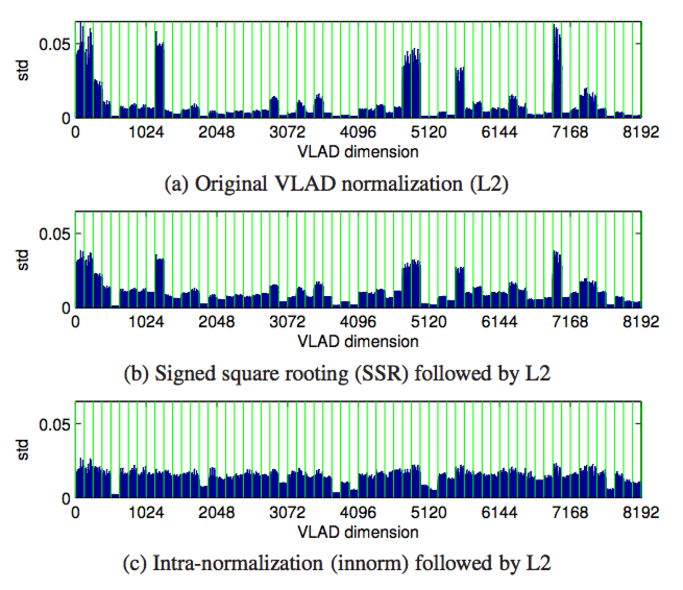
\includegraphics[height=8cm]{figures/vladnorm}
\end{center}
\caption{The effect of normalization on burstiness in VLAD dimension vs. standard deviation (std) which denotes amount of energy stored in that dimension. Clearly intra-normalization followed by L2 normalization evens out energy stored in different VLAD dimensions. Burstiness could result from a repeated structure in the image like a brick wall or a tiled floor for example. \cite{Arandjelovic2013}.}
\label{vladburstiness}
\end{figure}

In \cite{Arandjelovic2013}, Arandjelovi\'{c} and Zisserman modify VLAD in three ways to improve retrieval performance. First they decrease burstiness \cite{Jegou2009}, \cite{Delhumeau2013} (fig. \ref{vladburstiness}), few large components in the VLAD vector can dominate similarity computations. SSR normalization decreases burstiness but does not eliminate it. Intra-normalization alleviates burstiness and improves \emph{mAP} \cite{Arandjelovic2013}. Instead of L2-, or signed square root-normalizing over all descriptor blocks, the sum of the residuals within each VLAD block is normalized. Afterwards L2 normalization is carried out. Intra-normalization is very successful in repressing burstiness (fig. \ref{vladburstiness}).

Second, if the visual vocabulary is trained using one data set and used on another, the recognition performance suffers. Vocabulary adaptation in \cite{Arandjelovic2013} alleviates the symptoms without re-training the vocabulary, an expensive and inconvenient operation especially for large data sets. It would also require the storing of the original descriptors. \emph{Cluster center adaptation} uses $\hat{\mu}$ which are adapted to the mean of descriptors assigned to the same center $k$. The VLAD descriptors are then updated to use the new centers. Their assignment to a center does not change, but this makes comparing image similarity using VLAD more precise. Vocabulary adaptation and intra-normalization are orthogonal and may be used independently. Increases of as much as 34\% (fig. \ref{vladadapt}) may be observed using both vocabulary adaptation and intra-normalization. \cite{Arandjelovic2013}

\begin{figure}[htb]
\begin{center}
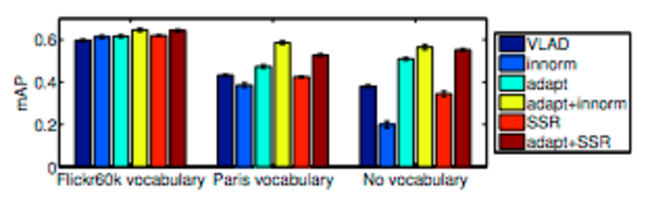
\includegraphics[height=2cm]{figures/vladadapt}
\end{center}
\caption{Comparing retrieval performance in the INRIA Holidays data set between VLAD, \emph{innorm} intra-normalization, \emph{adapt} vocabulary adaptation, \emph{adapt+innorm} is both vocabulary adaptation and intra-normalization. \cite{Arandjelovic2013}.}
\label{vladadapt}
\end{figure}
Third, VLAD loses to BoW in performance for objects occupying a small portion of the image. \cite{Arandjelovic2013} proposes \emph{Multiple VLAD descriptors} (MultiVLAD), which is especially useful in object recognition. MultiVLAD extracts a total of 14 VLAD descriptors from a single image. A $3 \times 3$ grid over the image gives $9$, $2 \times 2$ grid gives four and one for the whole image. This comes at the cost of memory but is still feasible on off the shelf hardware at ~28GB for 100 million images \cite{Arandjelovic2013}. MultiVLAD outperforms 1792-D (vocab. size) VLAD, but is found to be inferior for images that cover at least 20\% of the image \cite{Arandjelovic2013}.

\clearpage

\section{Near-Duplicate Image Detection} \label{NDID}
We expect the Local Features-classifier to outperform perceptual hashing for NDID. However, to begin implementing near similar image detection improvements we need to be certain Local Features with Bag-of-Visual-Words is an improvement over DCT-, and simple block mean- perceptual hashes by running simulations. We will the Paintings Dataset from \cite{Vedaldi2012} and a ThingLink Dataset sampled from ThingLink. Near-duplicates of the originals described in table \ref{modifiedimages} are generated via script. We also test the classifiers with images known not to be in the database, a subset from the Oxford Buildings Dataset \cite{PhilbinJamesArandjelovicReljaZisserman2012} for the Paintings Dataset and for the ThingLink Dataset we sample another equal size batch of images from the service. The ThingLink Dataset is used to gain insight into how these NDID systems perform on real world images. A -P-dataset is needed to probe the detector's ability to reject images not in the database. Originals are stored in the database and modifications used for test queries are in table \ref{modifiedimages}. We sample 446 images from ThingLink without duplicates as well as another 446 images to be the -P-dataset.

Computational cost is interesting weighing NDID systems against one another. We will record the hash calculation time for the perceptual hashes. For the Local Features NDID this means descriptor extraction and computation time. The query time is the other component of interest. We will record times for a single run for each dataset, for each NDID system and plot the results. Also, we will compare the memory requirements of each system via examining database size in memory, and memory usage during query.

We also need to know how the classifiers perform against one another, report and analyze the results. Receiver operating characteristics (ROC) (section \ref{ROCSection}) have been useful for visualizing classifier performance \cite{Fawcett2006}, however they were found not to be as precise and useful as PR curves by \cite{Davis2006}. More recently, precision and recall have been identified to be biased as they concentrate only on the +R and +P columns of the contingency matrix leaving out true negatives (TN) \cite{POWERS2011}.

\subsection{Simulations}
Paintings Dataset from the ''Recognition of object instances practical'' \cite{Vedaldi2012} is used and it's images are used to build a database. Perceptual hashes for these images are calculated and stored. Near-duplicate sets are formed using Imagemagick shell scripts. For each near-duplicate image, it is tested if a match can be found in the database using the Simple Hash the DCT Hash and the Local Features Classifier. A subset of the Oxford Buildings Dataset \cite{PhilbinJamesArandjelovicReljaZisserman2012} is used as a -P-dataset. These images are not expected to be found in the database. The results are reported in ROC space PR plots.

We must keep in mind that the simulations are for a relatively small amount of images. We are merely proving that a Local Features and Bag-of-Visual-Words Classifier improves on perceptual hashing for NDID. This information can then be used to make a decision on production implementation.

\subsubsection{Datasets}
We will use two datasets in this study. The Paintings Dataset and the ThingLink Dataset. The Paintings Dataset is from the ''Recognition of object instances practical'' \cite{Vedaldi2012} of a total of 1708 images (black and white images are excluded) will be used due to near ready scripts and image database for the local features case. The ThingLink Dataset is sampled from ThingLink.

An ImageMagick shell script generates the manipulated duplicates. 53\% and 83\% scales simulate multiple scales of the same image. Photo straightening is simulated by a 10\% rotation. For color manipulation so we will saturate the image by 50\%. Histogram normalization is quite a common operation, so we will use a normalized version of the image to try to find matches. To simulate image cropping, we crop from all sides by $10px$. Adding a border is simulated by making duplicates with a 10px border. Vertical and horizontal flips are excluded as we do not expect our classifiers to perform well on those and they are not realistic use cases for ThingLink.

To test for images not in the set we pick 1708 images from the Oxford Buildings Dataset \cite{PhilbinJamesArandjelovicReljaZisserman2012} and run those images against the paintings set. This should measure how good each classifier is at labelling predicted negative images correctly.

\def\arraystretch{1.5}
\begin{table}[htb]
\caption{Test image datasets from the ''Recognition of Object Instances Practical'' \cite{Vedaldi2012} paintings image set generated via shell scripts. Predicted negative set sampled in random from Oxford Buildings Dataset \cite{PhilbinJamesArandjelovicReljaZisserman2012}. The same procedure is run for the ThingLink dataset. -P images are also sampled from ThingLink.}
\label{modifiedimages}
\begin{center}
\begin{tabular}{lp{0.5\linewidth}}
  Modification & Motivation \\
  \hline \hline
  53\% Scale& Simulate responsive site case where image has a scaled duplicate. Choose prime percentage to avoid multiple of two to push scaler to produce uneven results.\\
  \hline
  83\% Scale& See above \\
  \hline
  Crop 10px & Simulate cropping image by 10px or removing a border for example\\
  \hline
  10\% Border & Adding a border to a known image \\
  \hline
  Rotate 10\% & User corrects the horizon of a photo \\
  \hline
  Normalize Histogram & User normalizes the histogram of a photo\\
  \hline
  Saturate Colors & User decides to modify the color palette of the image or photo\\
  \hline
  Predicted Negative & Does the system classify images correctly as not in database?\\
\end{tabular}
\end{center}\end{table}
\clearpage
The Paintings Dataset from \cite{Vedaldi2012} contains images of homogeneous quality and domain. Most notably, the Paintings Dataset contains a single pixel by pixel duplicate image. It was recognized that this duplicate image caused FP classification depending on which of the duplicates was sorted as the first item in the retrieved short list of images. Based on this finding, duplicates were removed from the ThingLink Dataset. The ThingLink Dataset consists of 446 images sampled from ThingLink. For this study, the ThingLink Dataset gives a base to compare the NDID methods with the types of images they are expected to work with in ThingLink production environment.

This imageset is heterogeneous in content containing landscapes, closeups of food, portraits and product brochures as well as ads. All of the files use lossy JPEG encoding. These images will form the predicted negative (-P) set forming the database. TP modifications are formed according to table \ref{modifiedimages}. A -P-dataset is needed to make sure images not in the database are reliably rejected by the classifiers. The -P-dataset is a more recent export of JPEG images from the service. These images are of varying size and content.

\subsubsection{Perceptual Hashing}
An image database is built and perceptual hashes in section \ref{perceptualhash} (Simple Hash and DCT Hash) are calculated by the exactly the same code running on ThingLink. For the hash distance function we will use Hamming Distance (section \ref{HammingSection}). We do not know how varying the Hamming Distance affects classifier performance. As a result we will run all sets for Hamming Distances of 0, 4, 8 \& 12 to find an optimal Hamming Distance for each perceptual hash. 10 was recommended by \cite{Zauner2010} but we want to know how these hashes perform on the paintings dataset and the ThingLink dataset. Images with dimensions exceeding 32px are ignored by the Simple Hash and DCT Hash algorithms. Having visual metadata for small images is counterproductive so they are ignored.
To query we use brute force to gather all the images in the database where the $\Delta(q,d)$ to the query image hash is less than or equal to $\Delta(q,d) \in \{0, 4, 8, 12$. We then return the result image where $\Delta(q,d)$ to the query is the smallest.
\subsubsection{Local Features for Near-Duplicate Image Detection}
We base our simulations heavily on the code from ''Recognition of Object Instances Practical'' \cite{Vedaldi2012}. Our contribution is to use a single result from the short list of matches return from a Large-Scale Image Retrieval query.

The ready trained vocabulary for the Paintings Dataset is used for Paintings queries. For the ThingLink Dataset, the vocabulary is trained using the original images, the images which the duplicates are based on.

The Local Features classifier in this case makes use of the SIFT-descriptor (section \ref{SIFTSection}) and quantization of the descriptor into visual words as well as the inverted index for querying. The index building process is in figure \ref{vedaldigenindex} and near-duplicate query process is found in figure \ref{vedaldiquery}. The code is modified for compatibility with Matlab 2015a.

Unexpectedly, the -P dataset on the Local Features-Classifier performed the worst with $FPR = 1$. Since the Local Features-Classifier always returned the images with the highest matching scores to the query, this was bound to happen. A cutoff score meaning ''query image not found in database'', a TN classification solves the issue but left the question of what to set the cutoff score to. The data was then used to find an optimal cutoff score $\mathcal{C}_s$.

In order to determine optimum cutoff, simulations were run setting the cutoff score from 1 to 19 and finding the optimum score, which turned out to be 19, the maximum score in the -P dataset. If returned matches from a search score less than $\mathcal{C_s}$, the image is classified as a $TN$.

\begin{figure}[htb]
\begin{center}
  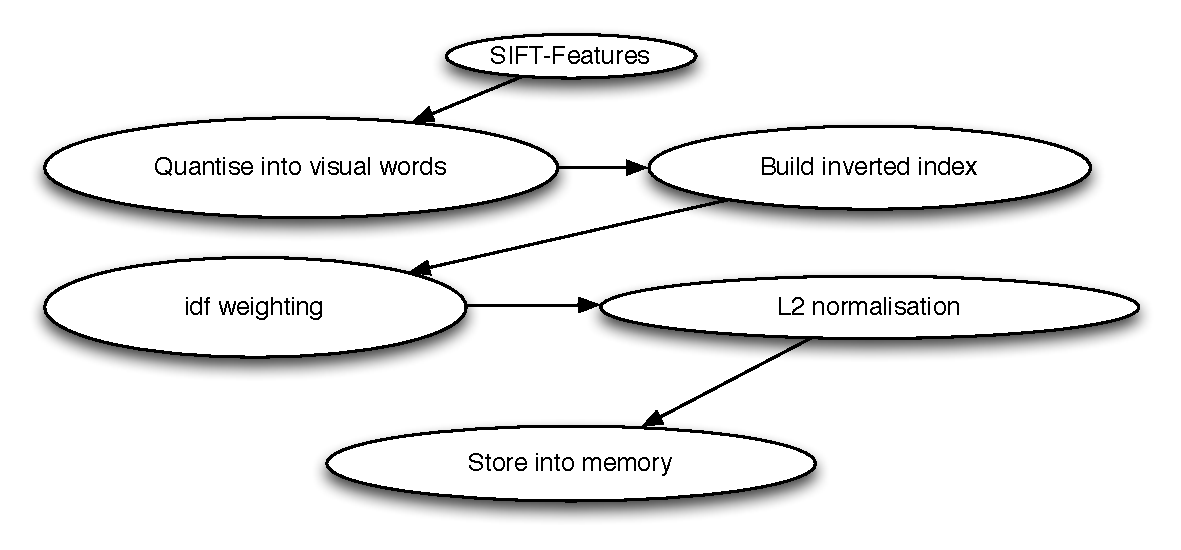
\includegraphics[height=7cm]{figures/vedaldigenindex}
\end{center}
\caption{Build image database for the local features-classifier simulations according to \cite{Vedaldi2012}}
\label{vedaldigenindex}
\end{figure}

\begin{figure}[htb]
\begin{center}
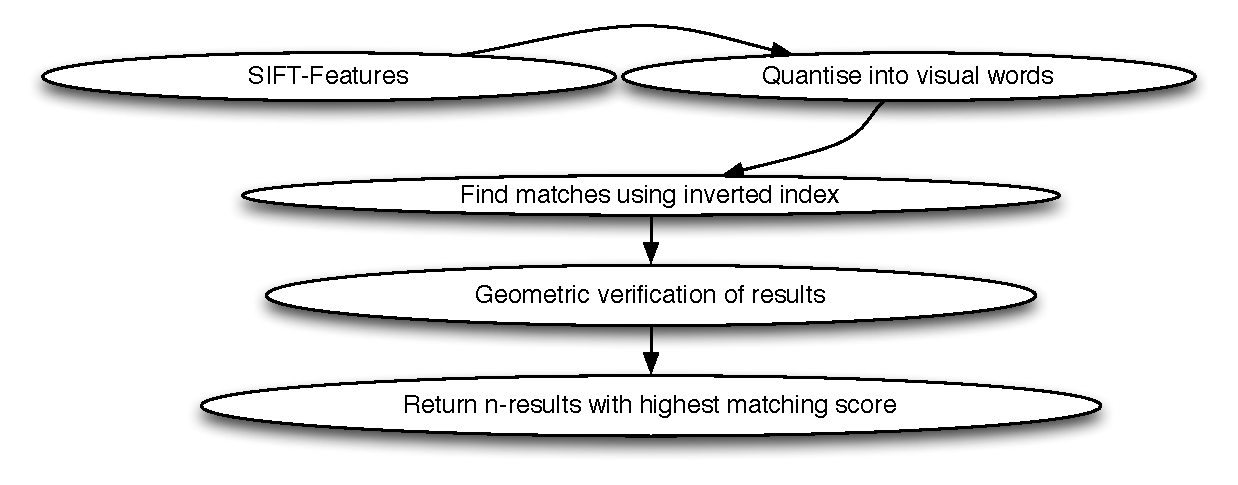
\includegraphics[height=6cm]{figures/vedaldiquery}
\end{center}
\caption{Image query in local features-classifier simulations according to \cite{Vedaldi2012}. For NDID $n=1$.}
\label{vedaldiquery}
\end{figure}

\subsubsection{Computational Cost}
Knowing roughly how much resources are needed for the NDID system is a basis for a rough cost estimate. CPU time and memory footprint of the hashes in the case of perceptual hashes and image descriptors for Local Features NDID. We will run the 53\% duplicate set and record the time it takes to calculate the descriptor/hash, the final memory footprint of the descriptor/hash. The query time for both the Paintings-, and the ThingLink datasets as well as the total database size in memory will also be recorded. The image databases are roughly $\frac{1}{3}$ in relative size so it should give insight into how computational cost of a single query varies with image database size. The system for these simulations is a Matlab version R2016a was used for simulations on an Intel Xeon E31230 3.20GHz with 8GB RAM on a 4.4.0 x86\_64 GNU/Linux Kernel.

For the perceptual hashes, the memory footprint for a single hash is well known to be 64 bits, the size of the hash. The size of the image database will be a multiple of this hash size. For the Local Features case, we will use the descriptor size of a single index in the inverted index, which contains one double for each word in the visual vocabulary, $1\times10^6$ words in our case. In addition to the descriptors the database contains metadata describing the descriptor database.

For these simulations, the metadata contains information on the original images like image name and download url and an id. In addition, a reference to the vocabulary $32 \times 128 \times 10^6$ bits is needed as well as the inverted index which needs vocabulary width per image of storage. The inverse document frequency reference for the entire vocabulary is $64 \times 10^6$.

\subsection{Binary Classification}
''A classifier is a mapping from instances to predicted classes'' \cite{Fawcett2006}. Near-duplicate image detection is an example of binary classification. A database of known images is queried by an incoming image. We are interested in finding a near-duplicate for the query image. If a near-duplicate exists in the database, we return that image and have a true positive (TP). In case a near duplicate image is retrieved and labeled a predicted positive, but the wrong image is returned from the database, we have a false positive (FP). When the query image is predicted positive but no near-duplicate image is returned, a false positive (FP). Given a predicted negative image query from the database and a near duplicate is returned, a false negative (FN) results. When a predicted negative image query returns nothing, a true negative (TN) results. We will use the approach in \cite{POWERS2011} and label counts in capital letters, such as TP, and probabilities in small letters for example \emph{tp}.
\begin{figure}[htb]
\begin{center}
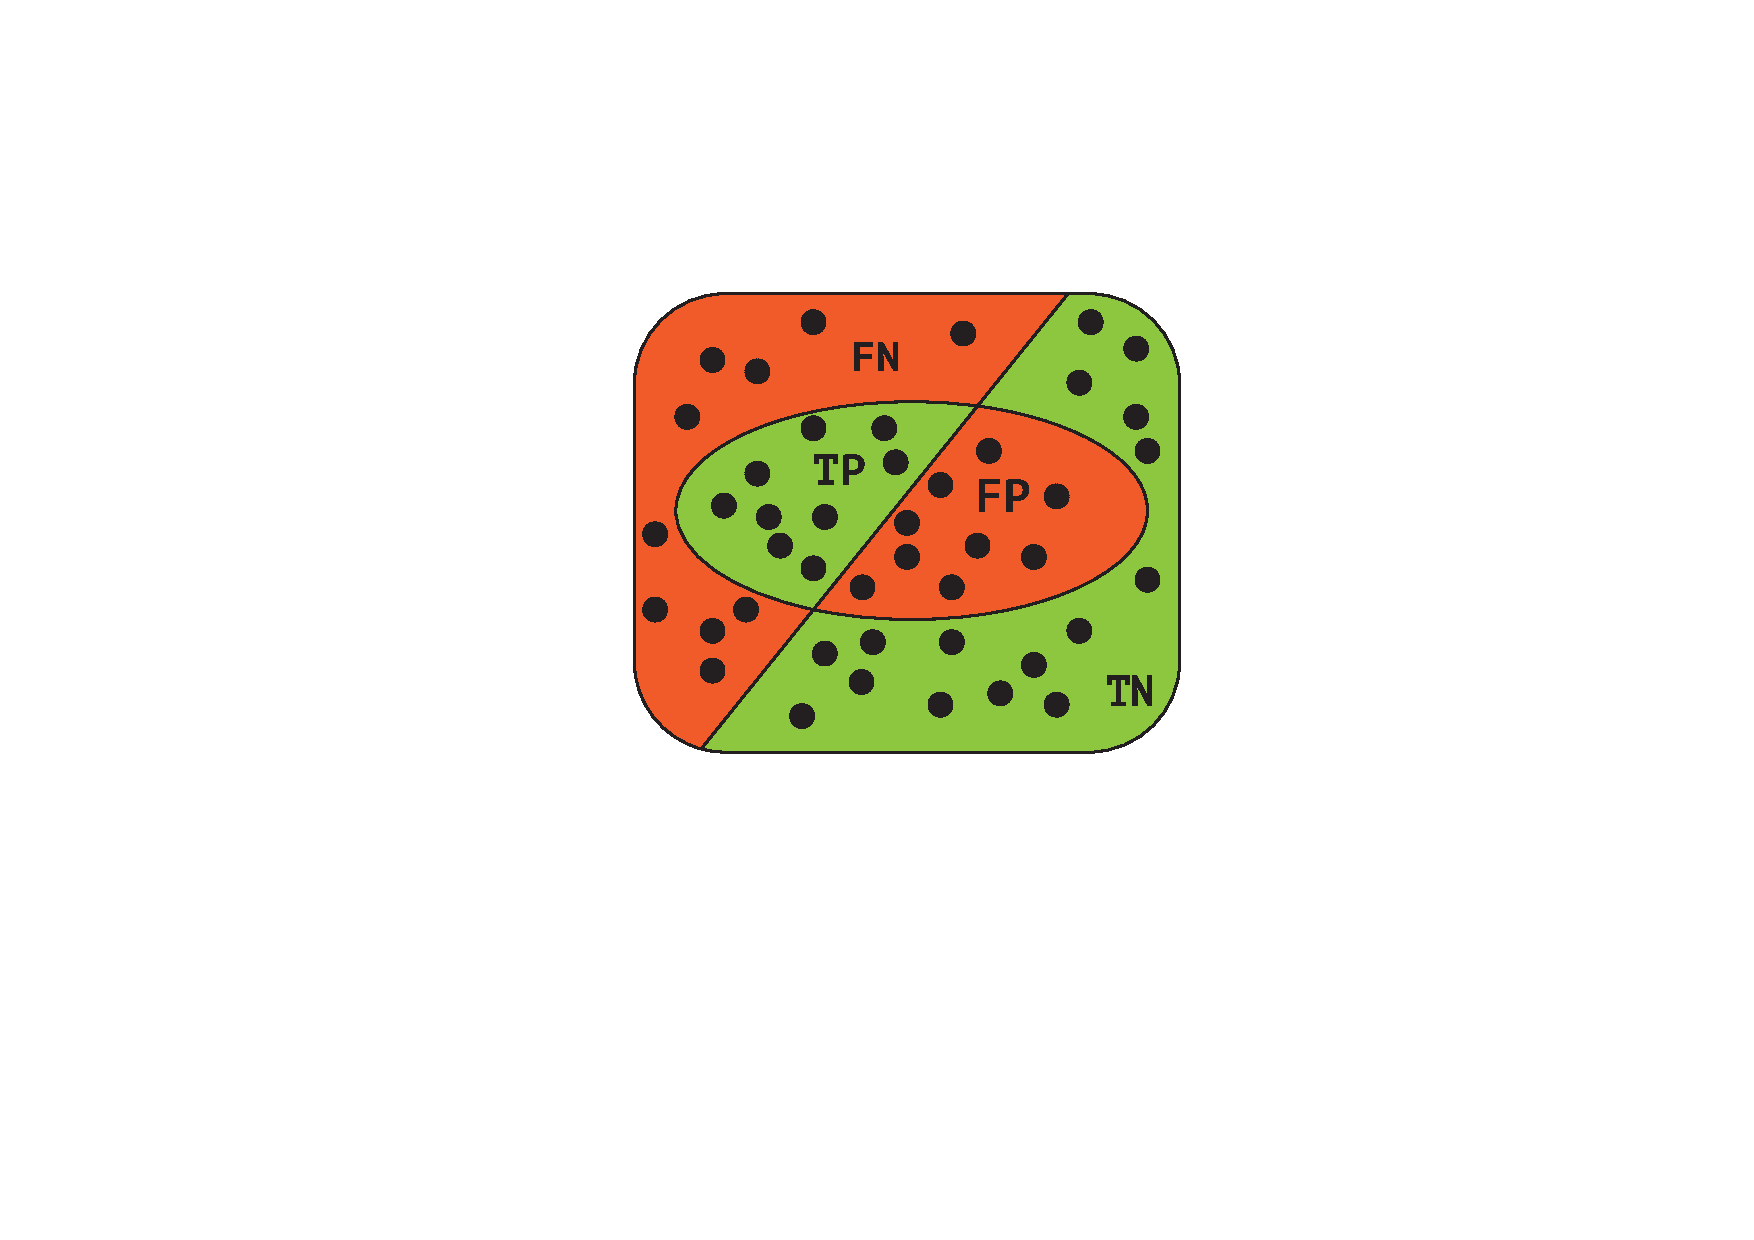
\includegraphics[height=6cm]{figures/contingency}
\end{center}
\caption{Contingency table for binary classification. Green areas are correctly classified. Red areas contain incorrectly classified items. \emph{TP, FP, TN, FN} total N, the size of the test set.}
\label{figcontingencytable}
\end{figure}
In essence, we compare three binary classifiers with known data. In our case the image is classified correctly by the classification system or it is not. This is a binary classification problem. The confusion matrix is outlined in fig. \ref{figconfusion}. To compare the DCT-, and simple perceptual hash classifiers to large scale image retrieval by SIFT features we need datasets, near-duplicate system implementations, simulation scripts and methods to evaluate the outcomes. ROC curves, Precision-Recall curves and the Matthews Correlation Coefficient all provide tools for comparing binary classifiers in a systematic manner. The Fisher Exact test is used to determine statistical significance of the results.

\newcommand{\RNum}[1]{\uppercase\expandafter{\romannumeral #1\relax}}
\subsubsection{Receiver Operating Characteristic}\label{ROCSection}
According to \cite{Fan2006} ''Receiver operating characteristic'' (ROC) was first used by World War \RNum{2} radar operators reading the radar screen to discriminate between signal and noise. ROC-curves visualize classifier performance by plotting FPR to TPR. The ideal system lies at $(0, 1)$ while $(1, 0)$ represents a system that fails at classifying everything. A random classifier will land somewhere on the positive diagonal as TPR = FPR. The negative diagonal
\begin{equation}\label{biastoprevalence}
tpr + c\times fpr=1
\end{equation}
matches Bias to Prevalence where skew is $c$ \cite{POWERS2011}. To compare classifiers in ROC space, we merely choose the point or the curve closest to the top left corner, the point (0, 1).
\begin{figure}[htb]
\begin{center}
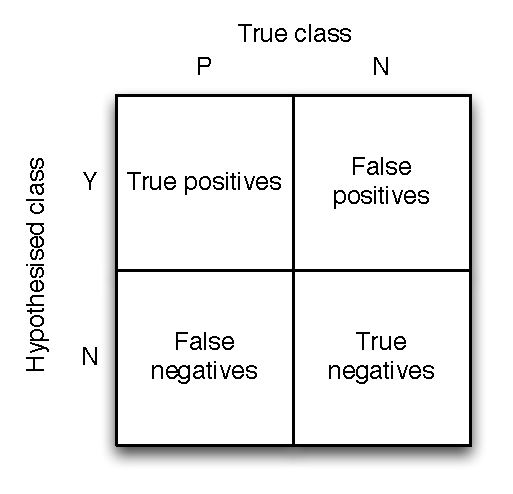
\includegraphics[height=8cm]{figures/confusion}
\end{center}
\caption{Contingency matrix for binary classification \cite{Fawcett2006}. Green denotes correct classification. Incorrect classification is in red. \emph{pp, pn, rp} and \emph{rn} are row or column probabilities and jointly sum to 1.}
\label{figconfusion}
\end{figure}

We adopt the notation from the ROC paper by Tom Fawcett and use ${Y,N}$ for output from the classifier. For true classification we use ${p,n}$ for positive and negative respectively. In case of a true positive $p$ is classified correctly as $Y$. A false positive is a $p$ classified as a $N$. A false negative is $p$ classified as $N$ and true negative is $n$ classified as $N$. ROC space in fig. \ref{figrocspace} is made by plotting the TPR vs. the FPR. The line from $(0,0)$ to $(1,1)$ represents classification by chance. Classifiers below this line do worse than luck itself. A discrete classifier outputs either $Y$ or $N$ or in our case image is found in the database or it is not. Discrete classifiers may be compared in ROC space like in fig. \ref{figrocspace} \cite{Fawcett2006}

\begin{figure}[htb]
\begin{center}
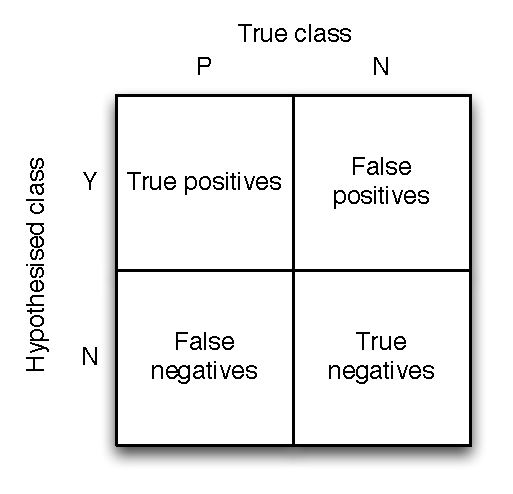
\includegraphics[height=8cm]{figures/ROC}
\end{center}
\caption{ROC space example with several discrete classifiers \cite{Fawcett2006}. }
\label{figrocspace}
\end{figure}

\setlength{\jot}{10pt}
\begin{align}
FPR &= \frac{FP}{FP + TN}\label{FPR}\\
TPR &= \frac{TP}{TP + FN}\label{TPR}\\
FNR &= \frac{FN}{RN}\label{FNR}\\
Precision &= \frac{TP}{TP + FP}\label{precision}\\
Recall &= \frac{TP}{TP + FN}\label{recall}\\
Accuracy &= \frac{TP +TN}{TP + FP + TN + FN}\label{accuracy}\\
F_1 &= \frac{2 \times TP}{TP + FP + 1}\label{fmeasure}
\end{align}
The f-measure (eq. \ref{fmeasure}) is the harmonic mean of precision (eq. \ref{precision}) and recall (eq. \ref{recall}). It has been used in to compare classifiers in document retrieval and machine learning.

\subsubsection{Precision-Recall}\label{PRSection}
Provost et al. warned of misleading reporting using accuracy (eq. \ref{accuracy}) alone to rate binary classifiers \cite{Provost1997} and recommended ROC curves in place of plain accuracy. ROC curves may give an overly optimistic view on an algorithms performance in the case of skew in the dataset even though ROC curves and PR curves contain the same points \cite{Davis2006}. Precision-Recall (PR) (eq. \ref{precision}, \ref{recall} respectively) curves have been suggested \cite{craven2005markov} to tackle comparison of classifiers in cases of data sets with skewed class distributions. In this paper we do not output probabilities of class values, merely if the image was identified correctly or not. In other words were interested in the correct image being retrieved if it is known to the system, or a clear indication that the image is not in the system. However, \cite{Davis2006} claim PR curves can expose differences between classifiers hidden in ROC space (fig. \ref{rocpr}).

\begin{figure}[htb]
\begin{center}
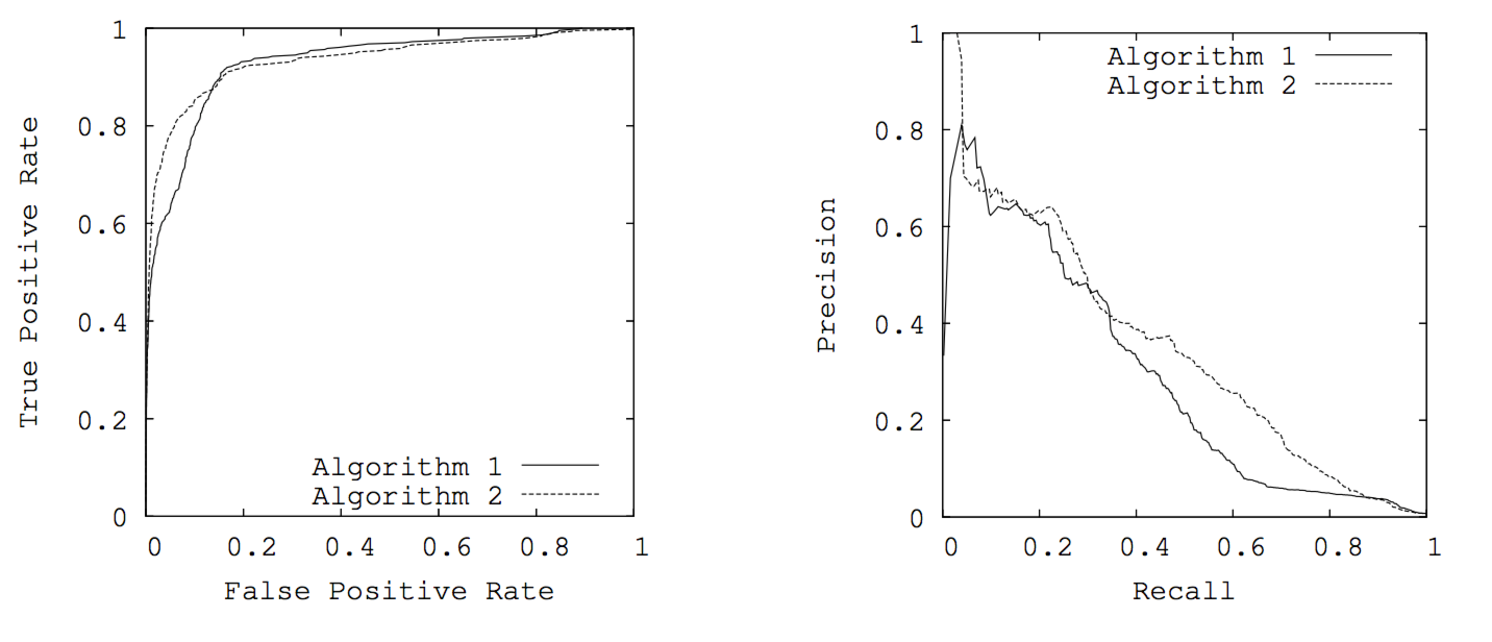
\includegraphics[height=6cm]{figures/rocpr}
\end{center}
\caption{ROC curve on the left and the corresponding PR curve on the right. \cite{Davis2006}}
\label{rocpr}
\end{figure}

Recall equals TPR (eq. \ref{recall}, \ref{TPR}) and precision is the TP-count over $TP \cup FP$ (eq. \ref{precision}). If recall $\neq 0$ then there exists a one-to-one correspondence between a ROC and PR curve \cite{Davis2006}. If a curve ''dominates another'' \cite{Provost1997}, that is is completely above the other curve in ROC space it doesn't mean this relationship is transferred into the PR curve. However, vice-versa relationship holds. If a curve dominates another in PR space it also dominates the other curve in ROC space. \cite{Davis2006}

As one can see from eq. \ref{precision} and \ref{recall} FN is absent from the PR representation. However, as it is the only term of four to be missing, and the other three parameters of the confusion matrix are known, it is trivial to solve for the fourth, FN in this case. \cite{Davis2006}

In ROC curves it is possible to linearly interpolate between points and the interpolations hold. However, in PR space linear interpolations do not hold and have to be calculated according to eq. \ref{printerpolate}. \cite{Davis2006}

\begin{equation}\label{printerpolate}
\left(\frac{TP_A+x}{Total Pos}, \frac{TP_A+x}{TP_A+x+FO_A+ \frac{FP_B-FP_A}{TP_B-TP_A}x} \right). \quad \cite{Davis2006}
\end{equation}

Precision, Recall, F-Factor, and Accuracy are biased and should be used only if these biases are well understood. Precision nor recall tells nothing about how well a model handles negative cases. \cite{POWERS2011}

The positive row and column of the contingency matrix (fig. \ref{figconfusion}) may be inversed to form statistics about the negative case. Inverse recall (eq. \ref{inverserecall}) is the fraction of real negatives that are predicted negative, which is analogous to the TNR. Inverse precision (eq. \ref{inverseprecision}) is the fraction of predicted negative cases classified as real negatives. \cite{POWERS2011}

\begin{align}
Recall^{-1} &= \frac{TN}{TN + FP}\label{inverserecall}\\
Precision^{-1} &= \frac{TN}{FN + TN} \label{inverseprecision}\\
Jaccard &= \frac{TP}{TP + FN + FP}\label{jaccard}\\
prevalence &= \frac{RP}{N}\label{prevalence}\\
bias &= \frac{PP}{N}\label{bias}\\
skew &= \frac{RN}{RP}\label{skew}
\end{align}
\emph{rp} is the Prevalence of positive cases. \emph{pp} on the other hand is the Bias of the model \cite{lafferty2001conditional}. $rp + rn = 1$, RP + RN = N. In a skewed distribution RN and RP are highly uneven resulting in many more negative errors than positive errors \cite{POWERS2011}.

An unbiased classifier accuracy was derived by Powers \cite{Powers2003} to avoid \emph{bias} and population prevalence. \emph{Informedness} (eq. \ref{informedness}) is a measure of intelligence in the model and indicates how informed a classification decision is compared to chance. For the binary case, it was first developed by Youden and is called Youden's J statistic. We will continue to use informedness, for this paper however. It may be used to find the optimum tuning on a ROC curve. \cite{POWERS2011}.
\begin{align}
Informedness &= 1 - fnr - fpr\label{informedness}\\
Markedness &= 1 - fpa - fna\label{markedness}
\end{align}
Markedness (eq. \ref{markedness}) is ''a measure of how consistently the outcome has the predictor as a marker by combining surfaces measures about what proportion of predictions are correct \cite{POWERS2011}''.
It has its roots in the psychology and linguistics. A marker or predictor (biomarker or neuromarker) is an indicator we use to determine how our classification task succeeded. For example, in our simulations, the filename of the image is a marker. If the retrieved file for a duplicate query is contained in the query image filename, we have a TP. The Pearson product-moment correlation coefficient $-1 \leq \rho \leq +1$ is a measure of linear dependence between two variables. The contingency matrix method for calculating $\rho$ is Matthews correlation $r_G$ which is the Geometric mean of \emph{Informedness} and \emph{Markedness}
\begin{equation}\label{matthewscorrelation}
r_G = \pm \sqrt{Informedness \times Markedness}
\end{equation}
The Matthews correlation can be seen as a joint probability of P informs R and R marks P \cite{POWERS2011}, on the condition that P to R prediction and R to P prediction are independent.
We will evaluate the classifiers against each other on the unbiased versions of \emph{Precision} which is \emph{Informedness} and \emph{Recall} which is \emph{Markedness} and the Matthews correlation.

\subsubsection{Statistical Significance}
To address statistical significance in comparing binary classifiers, the Simple Hash-, the DCT Hash- and Local Features NDID were essentially interested in addressing the significance of differences between classifiers. Fisher's Exact test is a good choice in literature. It can be used when the cell size is small. This is contrary to $\chi^2$, which needs every cell to have a count $>5$. Since the number of FP for the Local Features case is small, we expect to use the The Fisher Exact test, which was specifically designed for the analysis of statistical significance regarding contingency tables (fig. \ref{figconfusion}). As the name implies. The p-value is exact, and not an approximation. \cite{fisher1922interpretation}
However, Fisher's Exact Test assumes data to be hypergeometrically distributed meaning all assignments to the contingency matrix cells are considered equally likely, with Bias and Prevalence as given. However, since Bias and Prevalence are assigned as a result of the experiment, not before hand, the assumptions made by Fisher's Exact Test are inappropriate for this problem. We will keep this in mind when evaluating the p-values.
We will put the classifier results from the Local Features simulations in one row and the results from either DCT-, or Simple Hash NDID on the other row and run the Fisher Exact test. The null hypothesis $H_0$ is ''the systems are the same'' and we will use $\alpha < 0.05$ meaning the $H_0$ is rejected if it's probability based on the results is less than 5\%.

\clearpage

\section{Results}\label{results}
To what degree if any are Local Features an improvement over DCT-, and simple block mean based- perceptual hashes for near-duplicate image detection? To find out, modified image sets in table \ref{modifiedimages} for the Paintings dataset and ThingLink datasets were queried separately against the three NDID systems- the Simple Hash-, the DCT Hash- and Local Features-based systems. Near-duplicate detection was treated as a binary classification problem resulting in a contingency matrix for each dataset and each near-duplicate type at each parameter value.

For each perceptual hash the parameter was $\Delta(q,d) \in {0,4,8,12}$. Each run results in a single point in ROC and PR spaces. What is a good $\Delta(q,d)$ for the DCT- and Simple hashes for NDID? By visually examining ROC- and PR curves in figures \ref{53roc} - \ref{Saturateprthinglink} we can draw conclusions for a good $\Delta(q,d)$ and verify the results using \emph{informedness} $\mathcal{I}$, \emph{markedness} $\mathcal{M}$ and \emph{Matthews correlation} $\mathcal{R}_G$ in tables \ref{simpleunbiased} and \ref{simplethinglinkunbiased} for the simple hash. Tables \ref{dctunbiased} contain the DCT Hash $\mathcal{I}$, $\mathcal{M}$ and $\mathcal{R}_G$ for the Paintings Dataset. The ThingLink Dataset unbiased metrics are in table \ref{dctthinglinkunbiased}.

In the Local Features case, the query returns a list of images along with scores describing how many visual words an image in the database has in common with the query image. We choose the highest scoring image for consideration as a near-duplicate.
For the Local Features classifier, the tuning parameter was the cutoff score $0 \leq \mathcal{C}_s \leq \mathcal{C}_{s_{max}}^{-P}$ where $\mathcal{C}_{s_{max}}^{-P}$ is the maximum score from querying the -P dataset. What is a good $\mathcal{C}_s$ to reject an image, or in other words to classify an incoming image a TN?  A run at each $\mathcal{C}_s$ results in a point in ROC and PR plots in figures \ref{53roc} - \ref{Saturateprthinglink} along with perceptual hash results for easy visual comparison.

Simple Hash $\Delta(q,d)=4$ and the DCT Hash $\Delta(q,d)=4$ for head to head NDID system comparisons. $\mathcal{C}_s=19$ for Local Features NDID and the Paintings dataset and $\mathcal{C}_s=16$. To numerically compare the systems, unbiased equivalents of precision (Informedness $\mathcal{I}$) and recall (Markedness $\mathcal{M}$) values were calculated (table \ref{informednessmarkedness}) for a second opinion to visually comparing the classifiers in the ROC and PR plots in figures \ref{53roc} - \ref{Saturateprthinglink}. In order to make the differences in unbiased metrics explicit, we calculate deltas (table. \ref{deltainformednessmarkedness}) between Local Features and the perceptual hashes. For statistical significance of the differences between Local Features and the perceptual hashes for each dataset and near-duplicate type, we calculate the p-values (table \ref{pvalues}) using Fisher's exact test.

For computational resources (table \ref{computationalcost}) we are interested in the average CPU time $t_f^{avg}$ for calculating a perceptual hash, or an image descriptor and the average query time $t_q^{avg}$ to find a duplicate. For memory, we measured the size of a single hash or an image descriptor and the total image database with metadata included, like the visual vocabulary for example.

\begin{figure}[htb]
  \begin{center}
  \begin{subfigure}[b]{0.49\textwidth}
    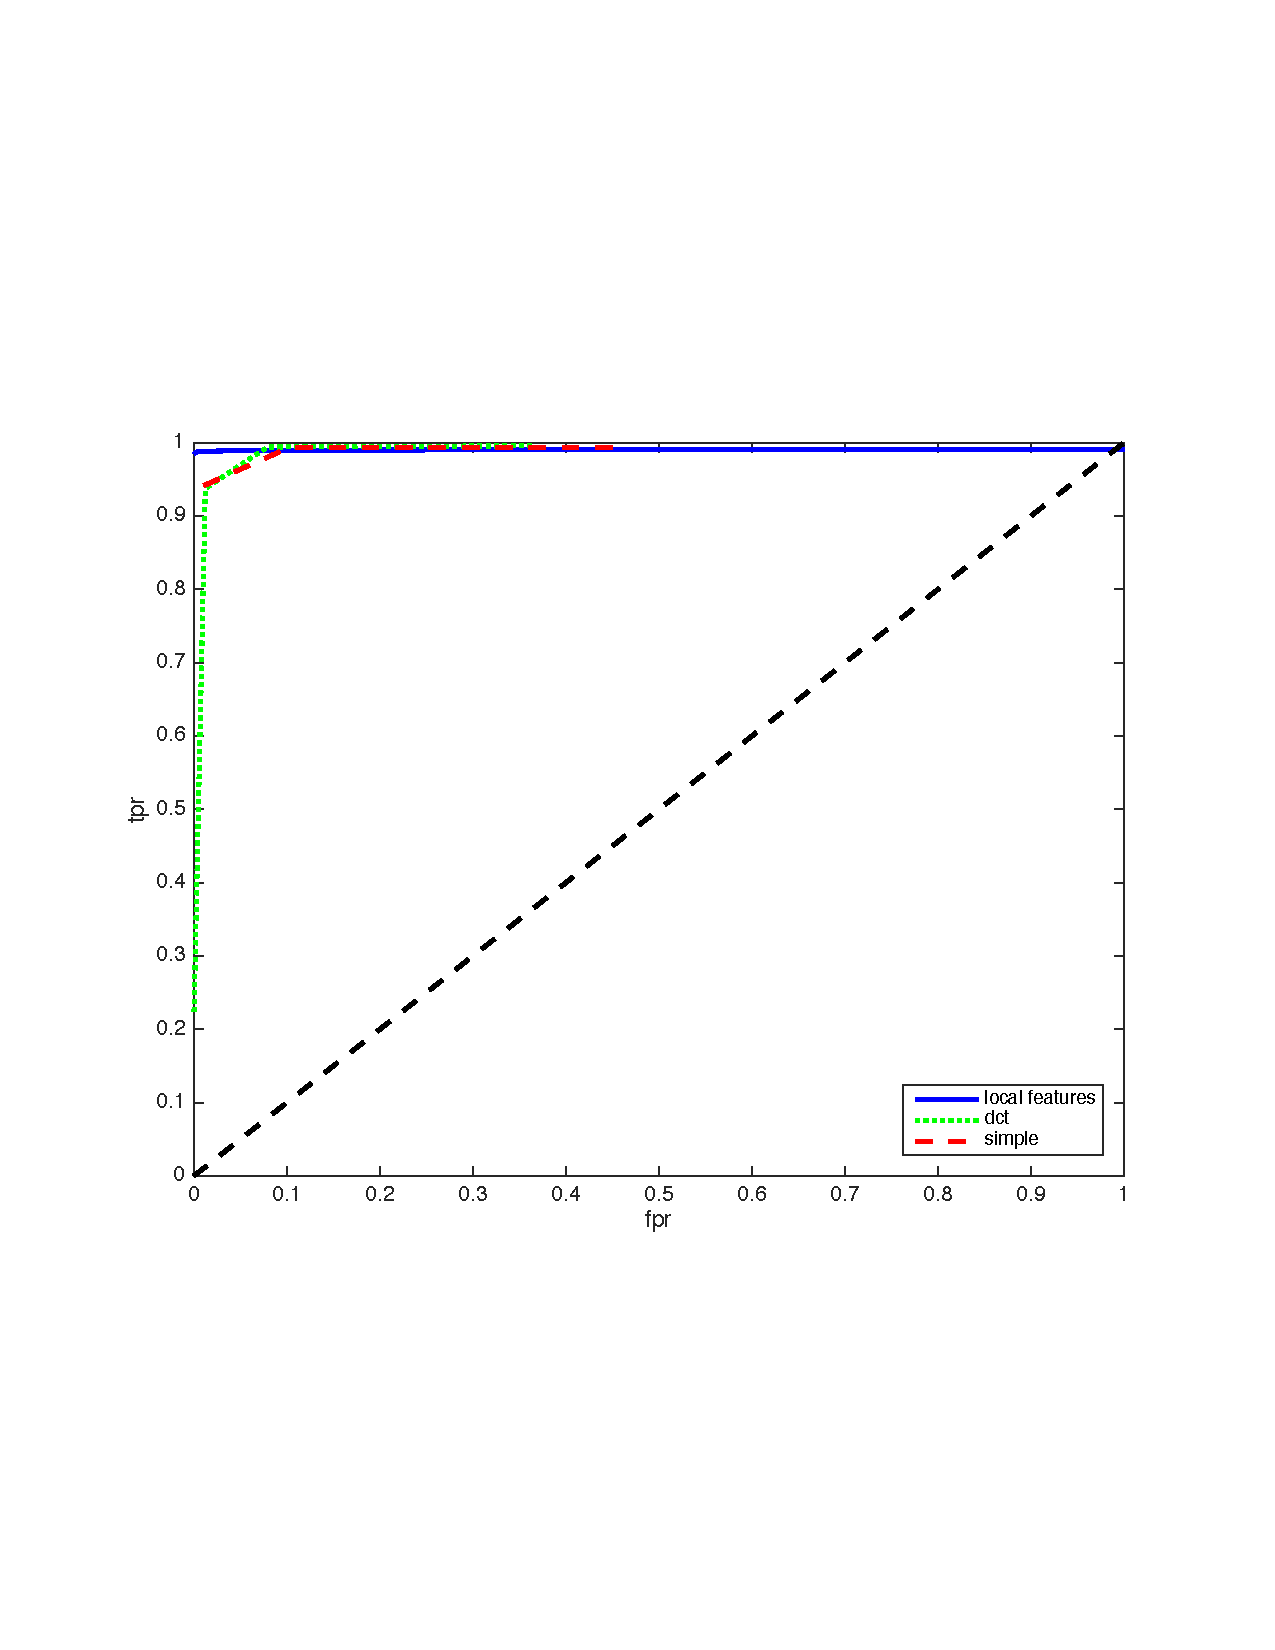
\includegraphics[width=\textwidth]{figures/53scaleROC.pdf}
    \caption{Paintings ROC}
    \label{53roc}
  \end{subfigure}
  %
  \begin{subfigure}[b]{0.49\textwidth}
    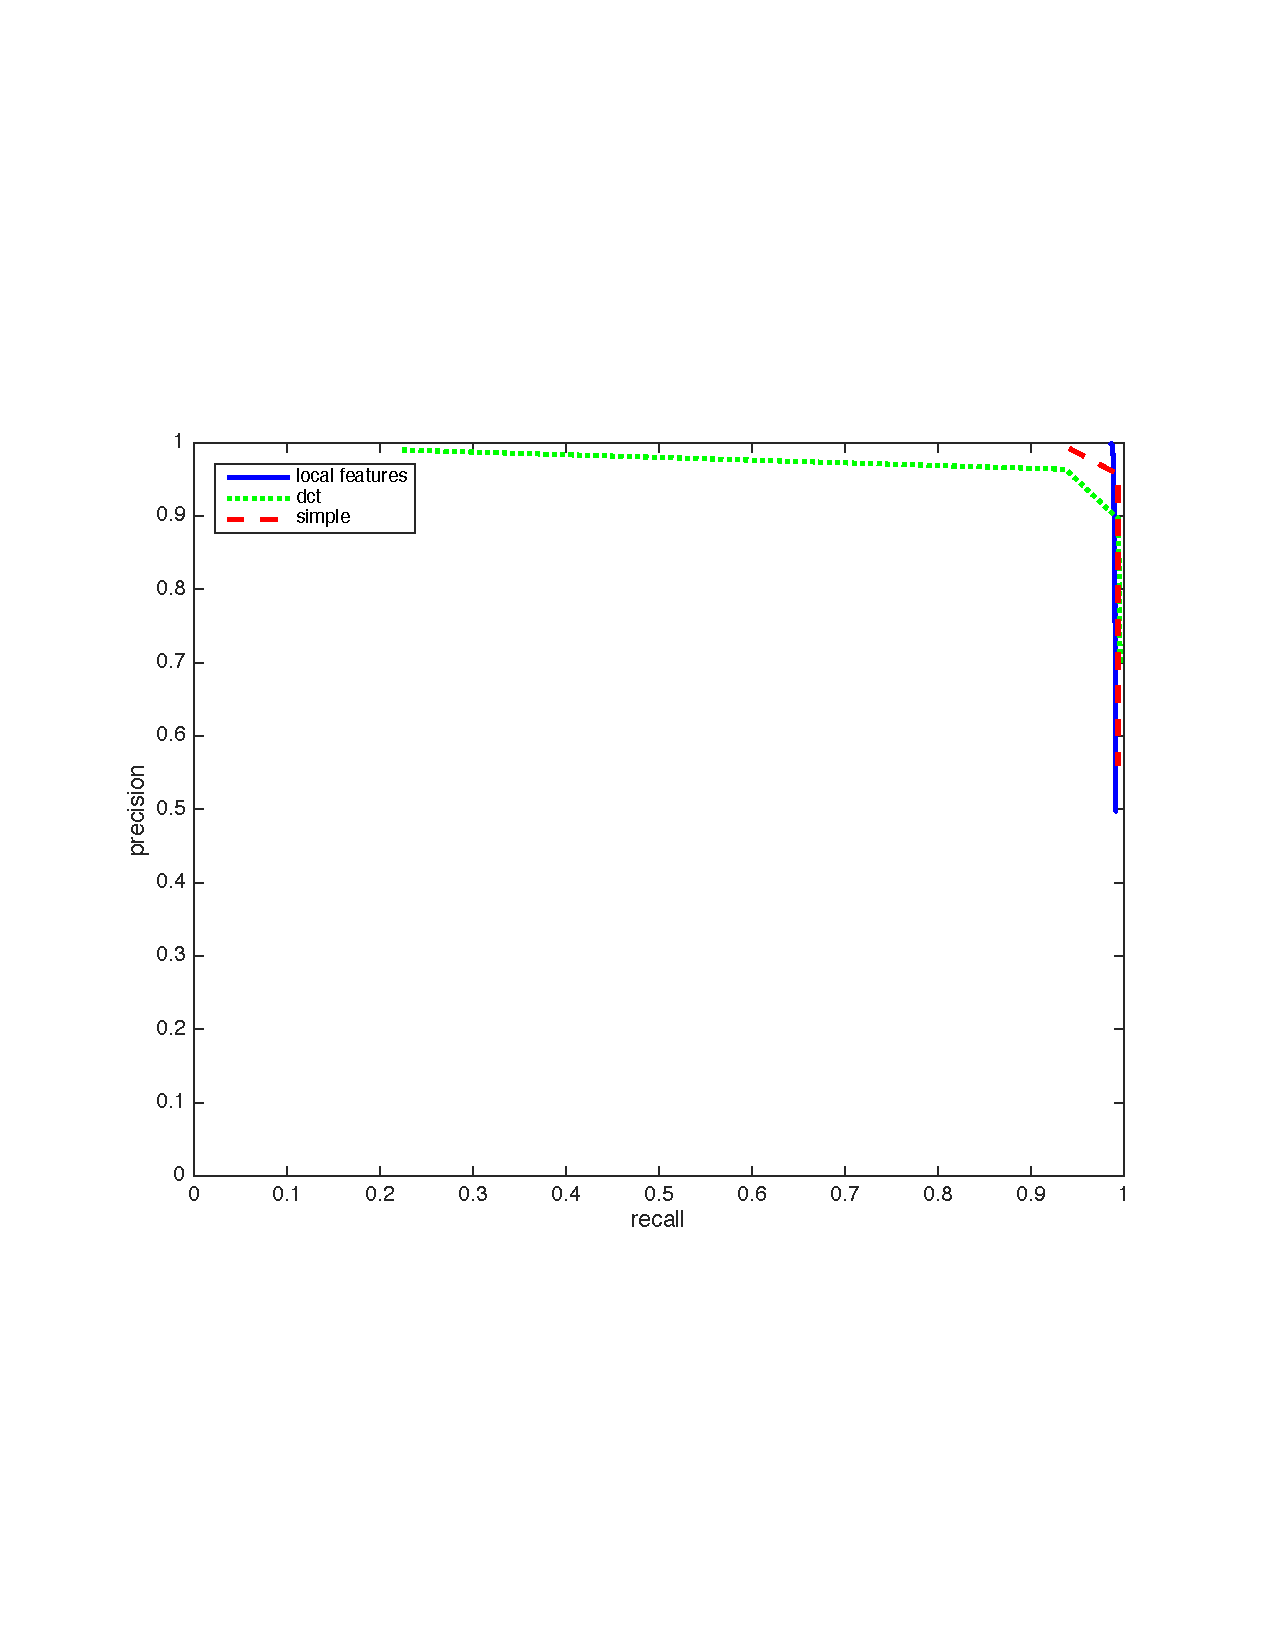
\includegraphics[width=\textwidth]{figures/53scalePR.pdf}
    \caption{Paintings PR}
    \label{53rocthinglink}
  \end{subfigure}
  \begin{subfigure}[b]{0.49\textwidth}
    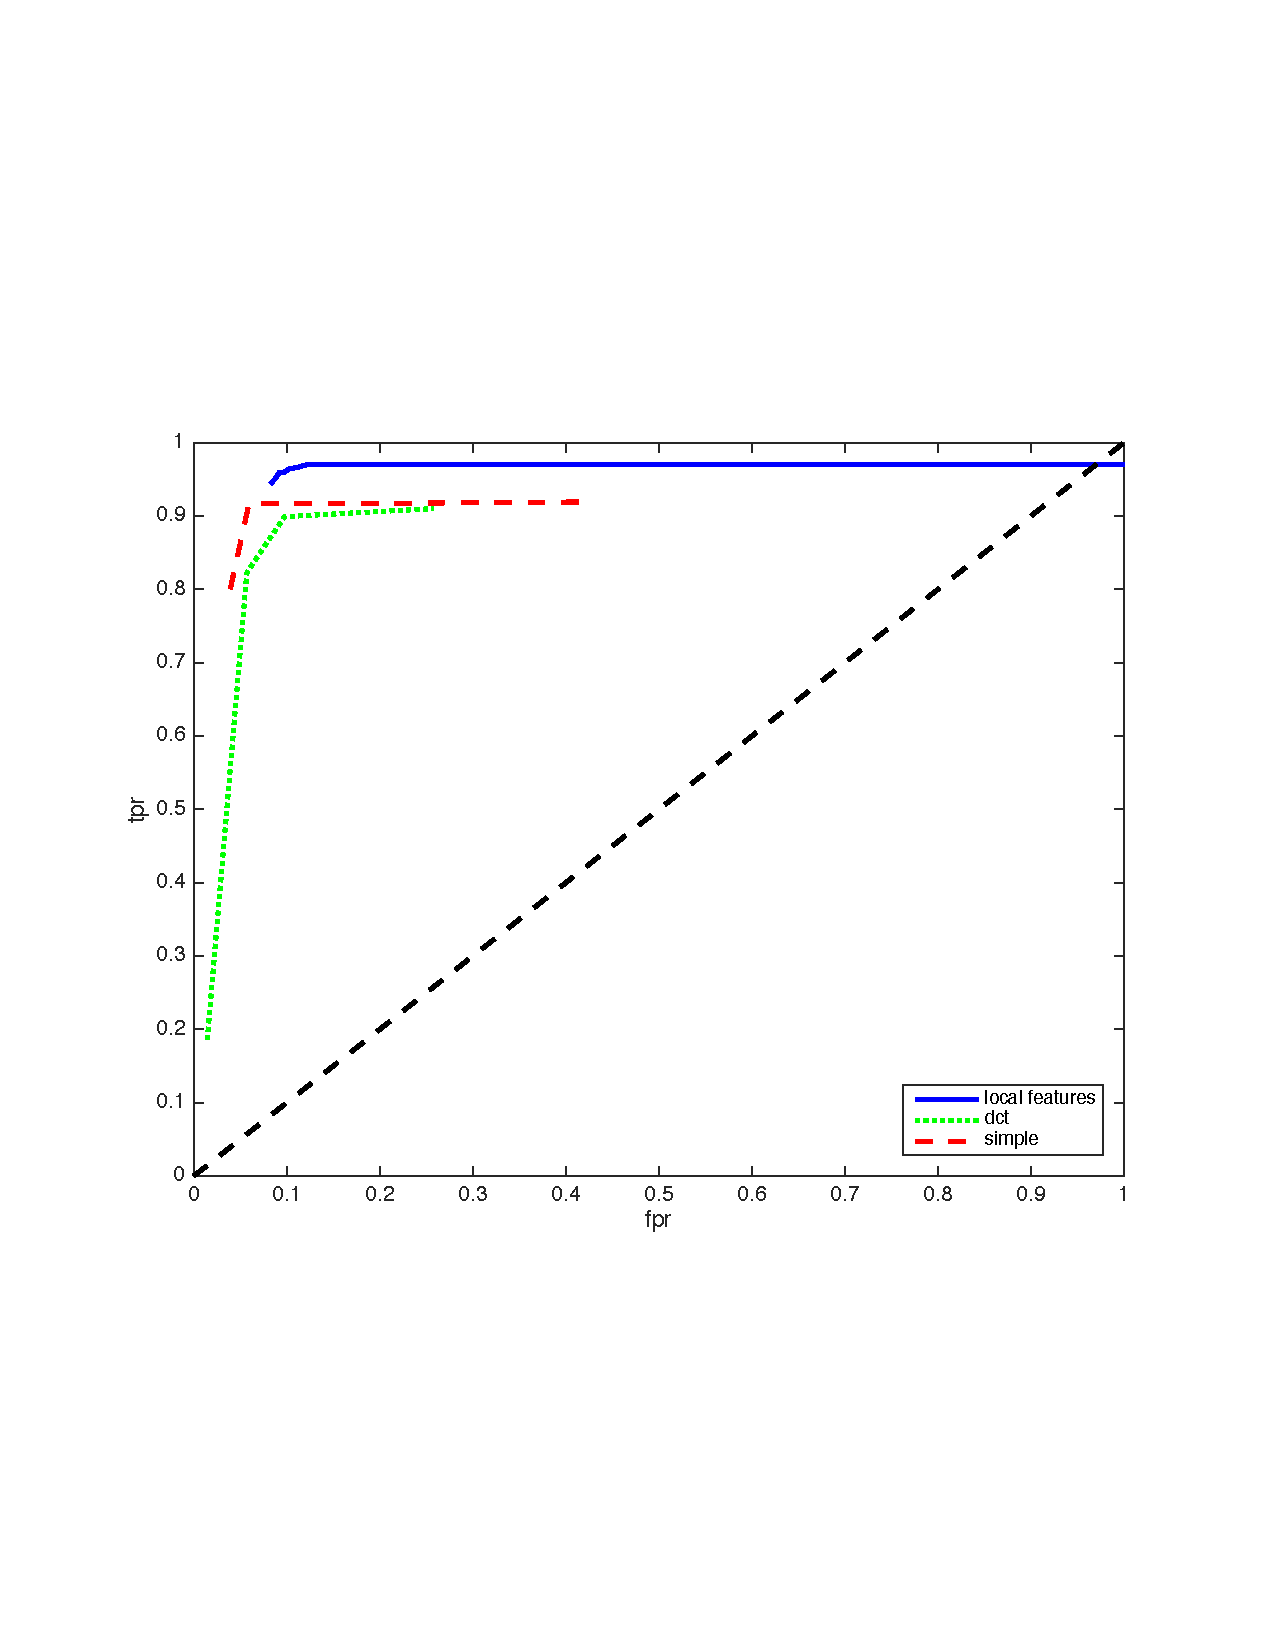
\includegraphics[width=\textwidth]{figures/thinglink_53scaleROC.pdf}
    \caption{ThingLink ROC}
    \label{53pr}
  \end{subfigure}
  %
  \begin{subfigure}[b]{0.49\textwidth}
    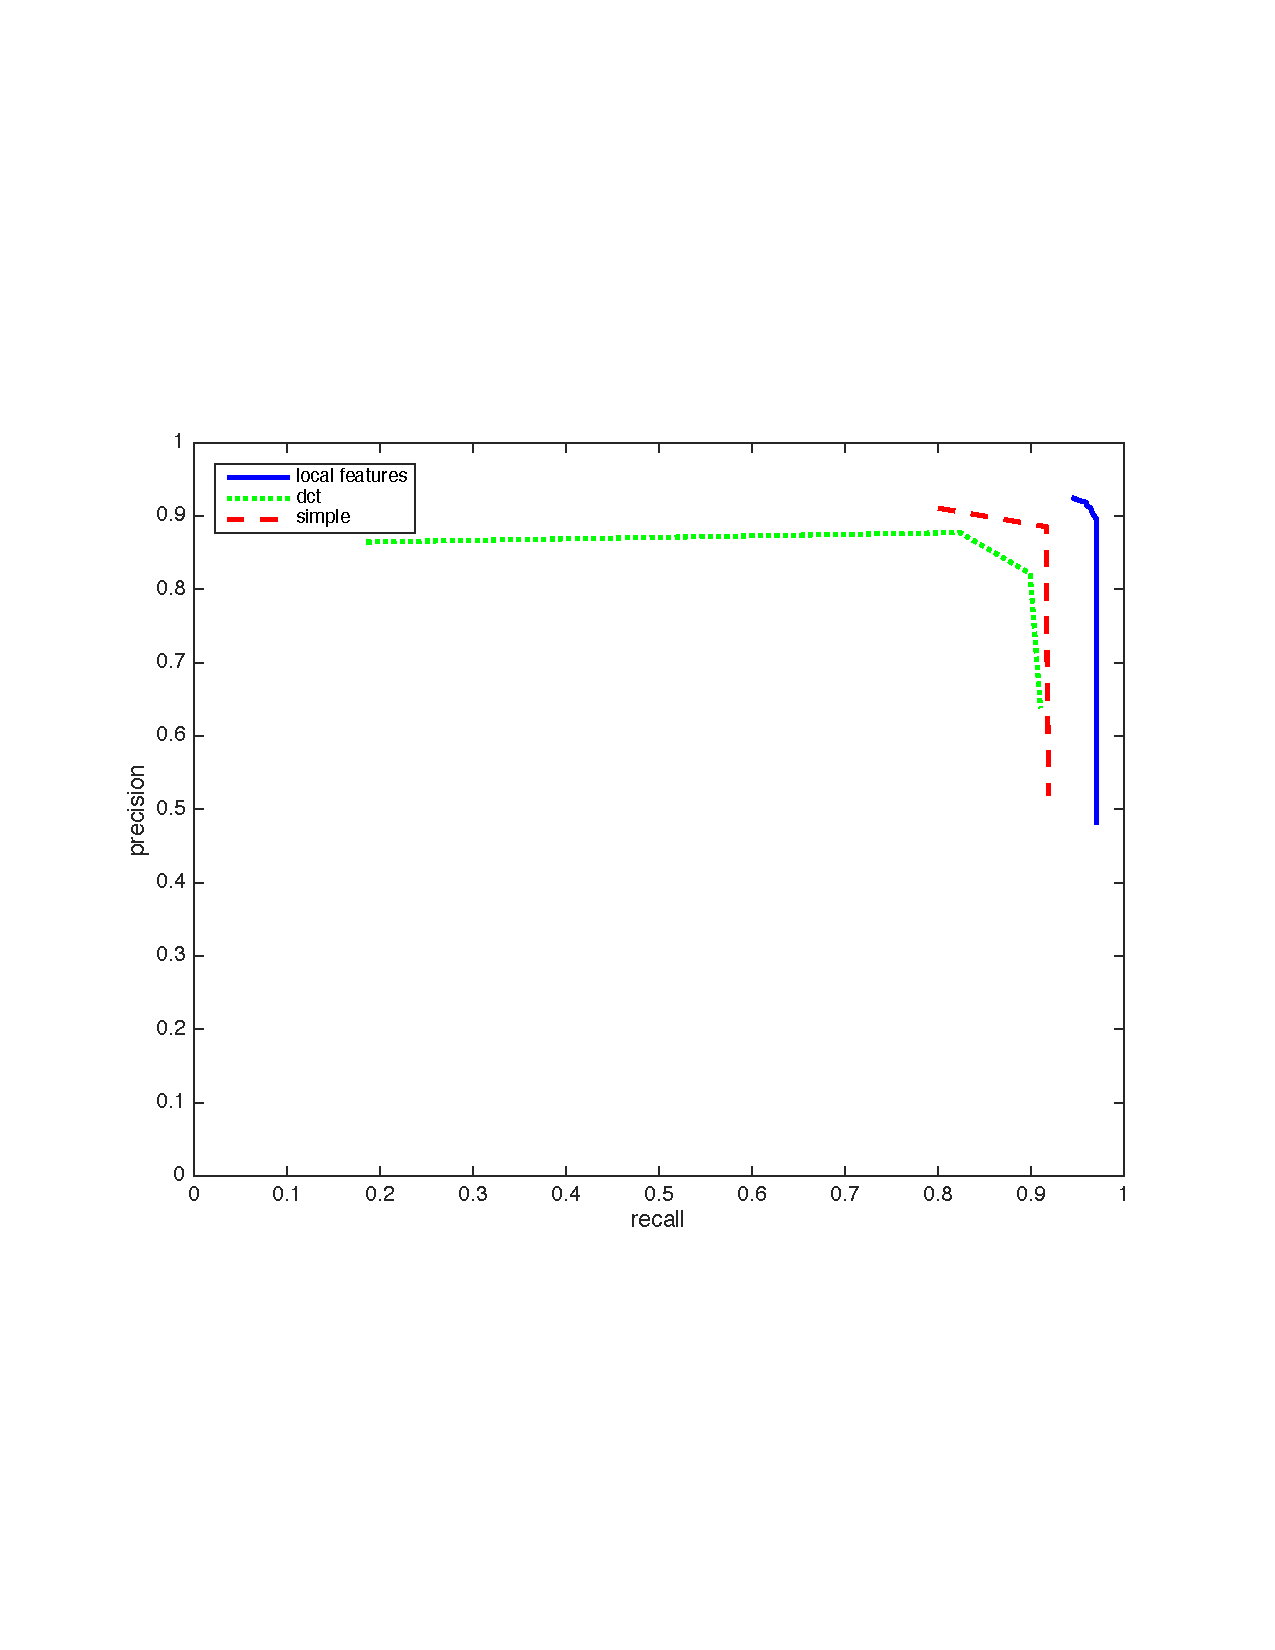
\includegraphics[width=\textwidth]{figures/thinglink_53scalePR.pdf}
    \caption{ThingLink PR}
    \label{53prthinglink}
  \end{subfigure}
  \caption{\emph{53\% scale near-duplicate query results}. Each point for the DCT- (green and dotted) and Simple Hashes (red and dashed) is for a given $\Delta(q,d) \in \{0,4,8,12\}$. $\Delta(q,d)$ increasing from left to right in ROC space and PR space. Each point for Local Features (blue and solid) is for a given cutoff score $0 \leq \mathcal{C}_s \leq 19$ for Paintings Dataset and $0 \leq \mathcal{C}_s \leq 16$ for the ThingLink Dataset increasing from right to left. The $\mathcal{C}_s$ interval between the points is 1. The leftmost point (topmost point in PR space) corresponds to $\mathcal{C}_s=19$ for the Paintings Dataset and $\mathcal{C}_s=16$ for the ThingLink Dataset. The rightmost point (the lowest point in PR space) is for $\mathcal{C}_s = 0$ for ROC. We acknowledge we have not interpolated between points in PR space according to eq. \ref{printerpolate} but draw a straight line as the distortion is minimal. The black dashed diagonal line in ROC space represents classification performance equivalent to flipping a coin and classifying accordingly.\label{53label}}
  \end{center}

\end{figure}

\clearpage
\begin{figure}[htb]
  \begin{center}
  \begin{subfigure}[b]{0.49\textwidth}
    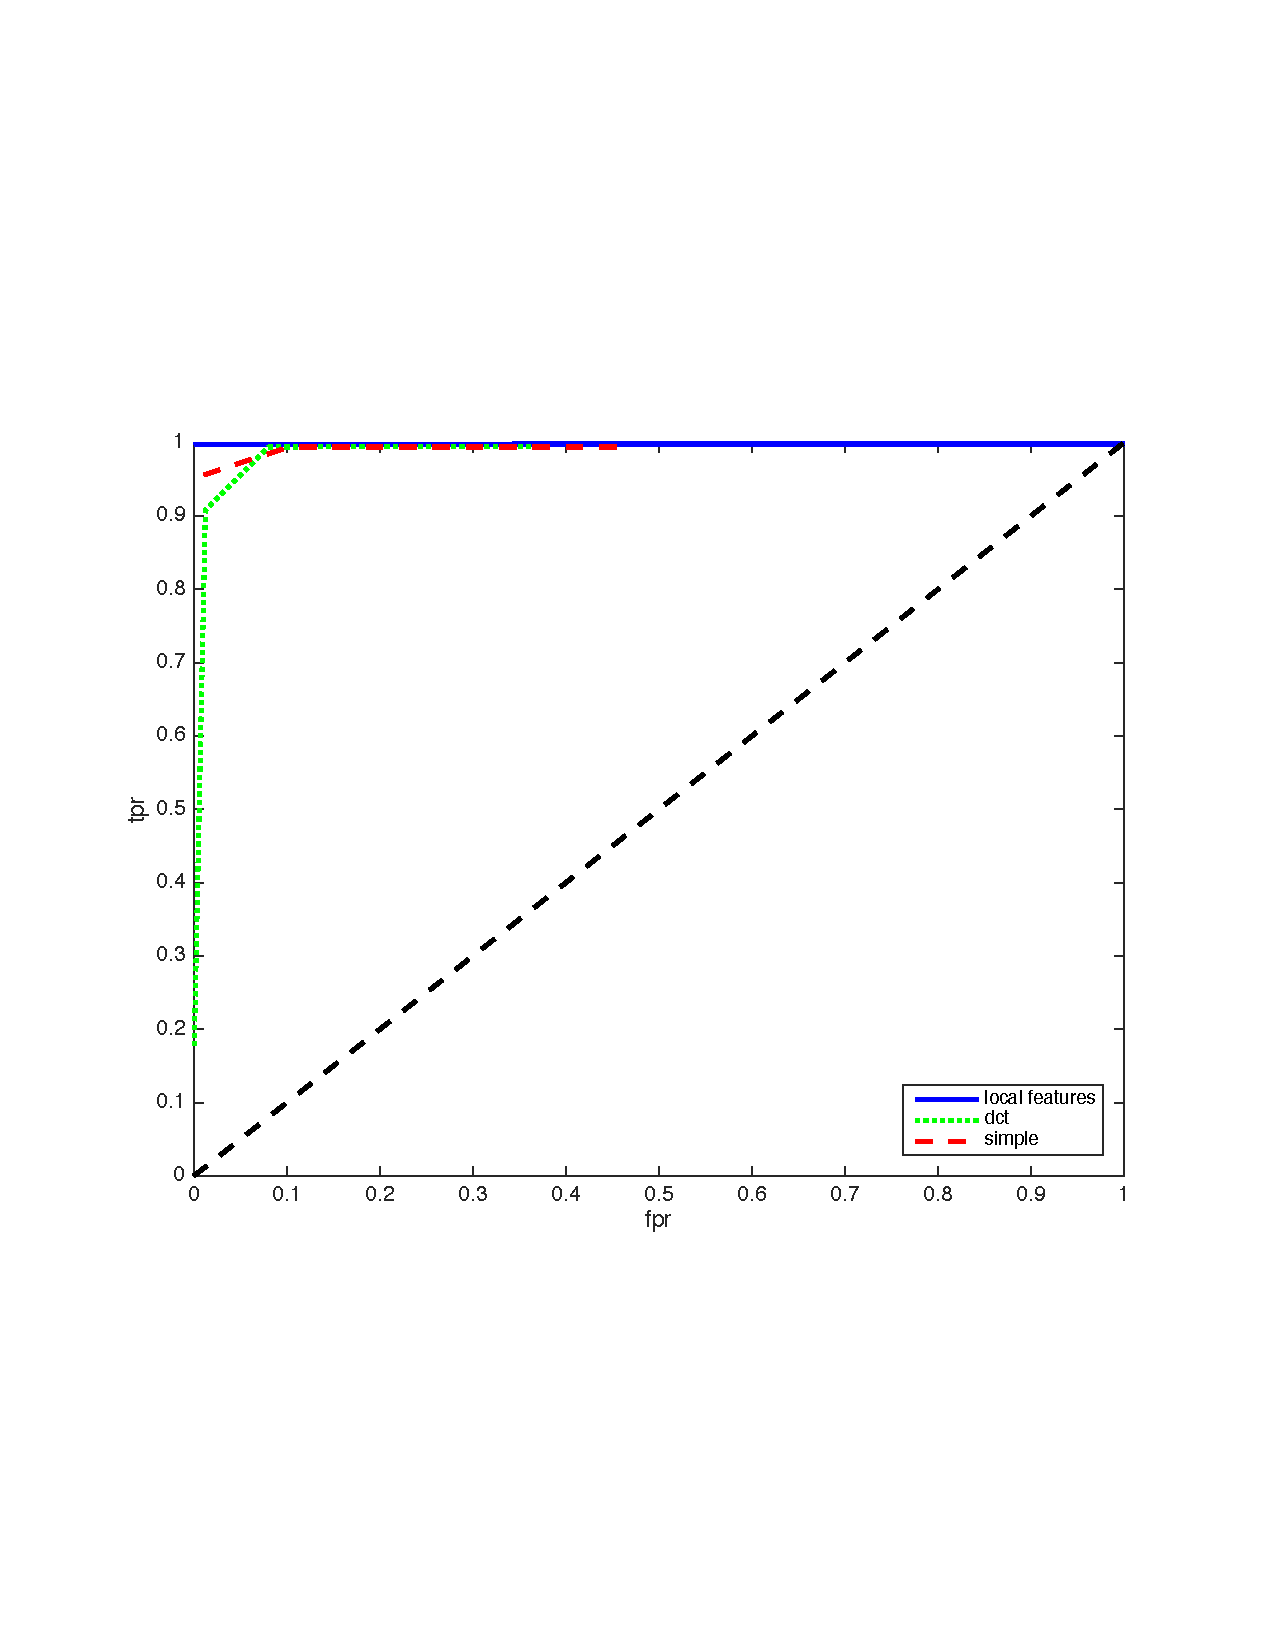
\includegraphics[width=\textwidth]{figures/83scaleROC.pdf}
    \caption{Paintings ROC}
    \label{83roc}
  \end{subfigure}
  %
  \begin{subfigure}[b]{0.49\textwidth}
    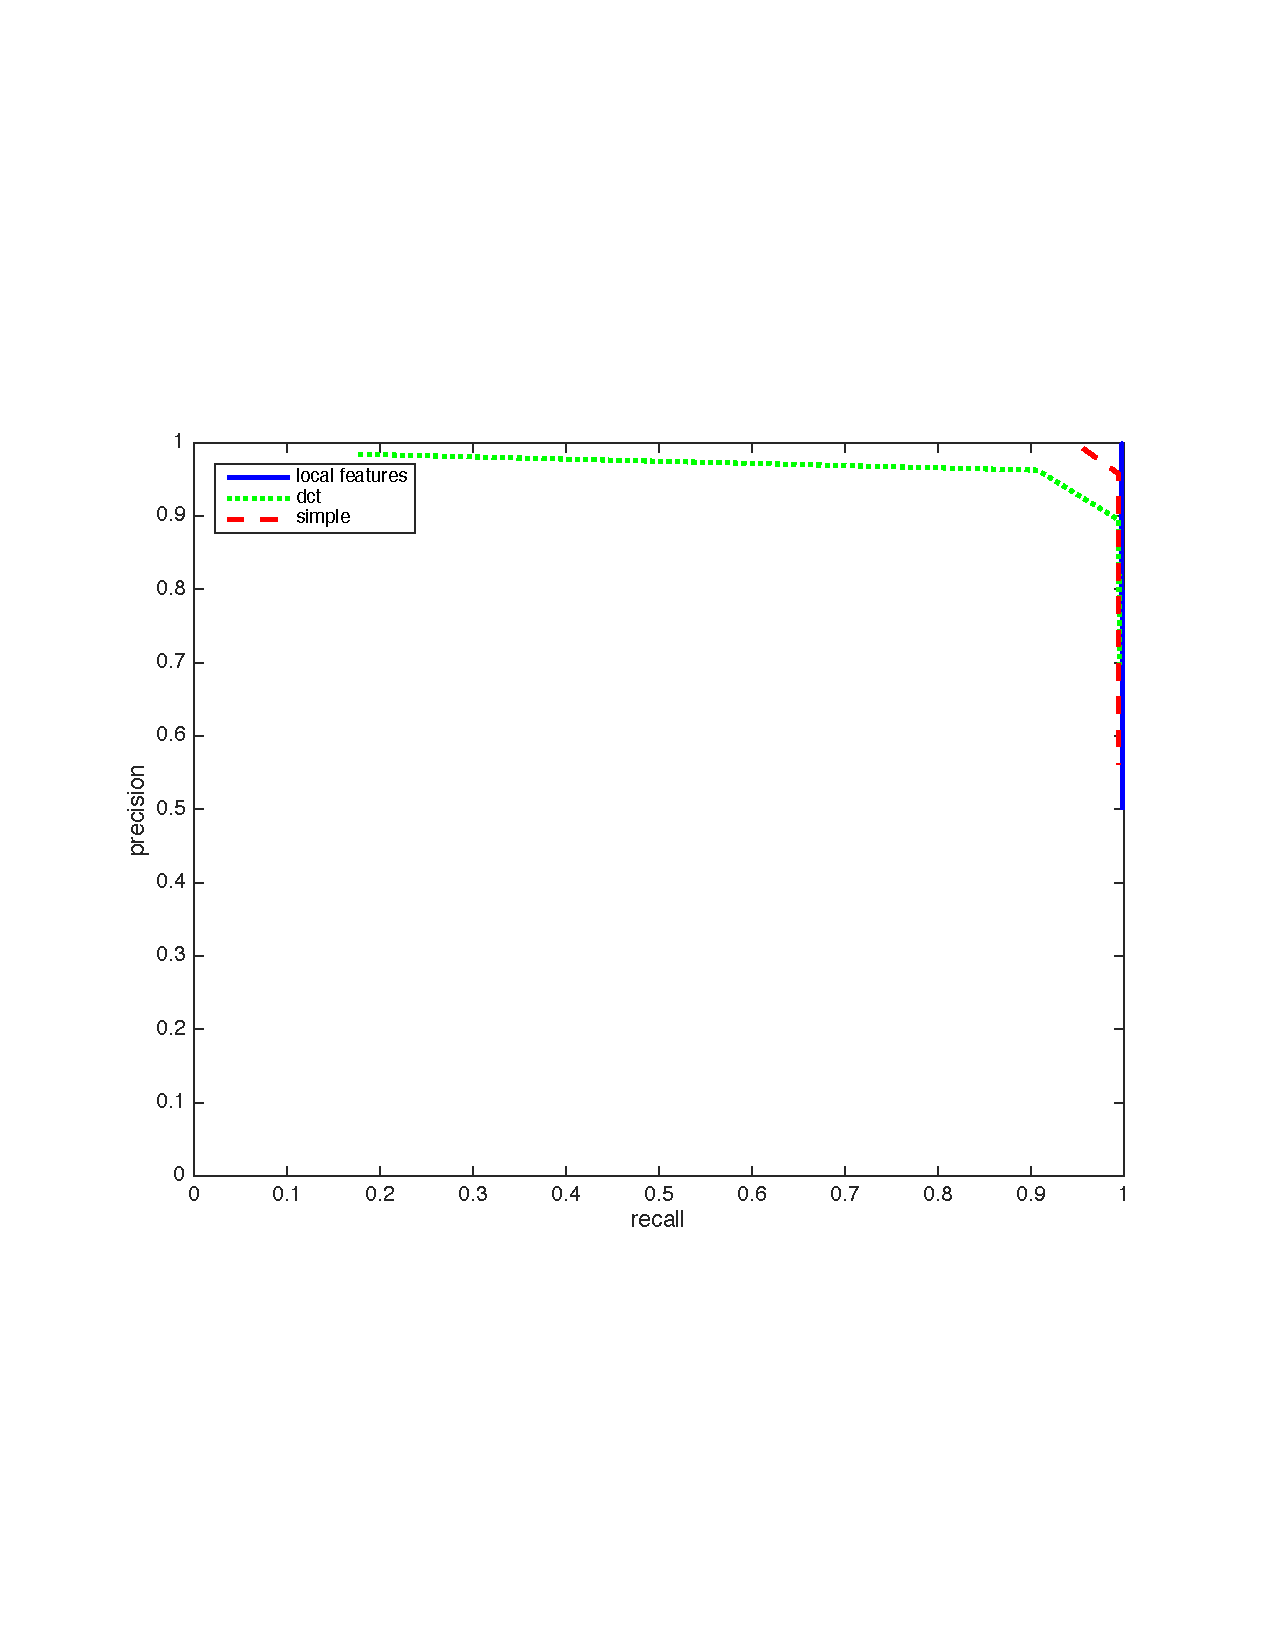
\includegraphics[width=\textwidth]{figures/83scalePR.pdf}
    \caption{Paintings PR}
    \label{83rocthinglink}
  \end{subfigure}
  \begin{subfigure}[b]{0.49\textwidth}
    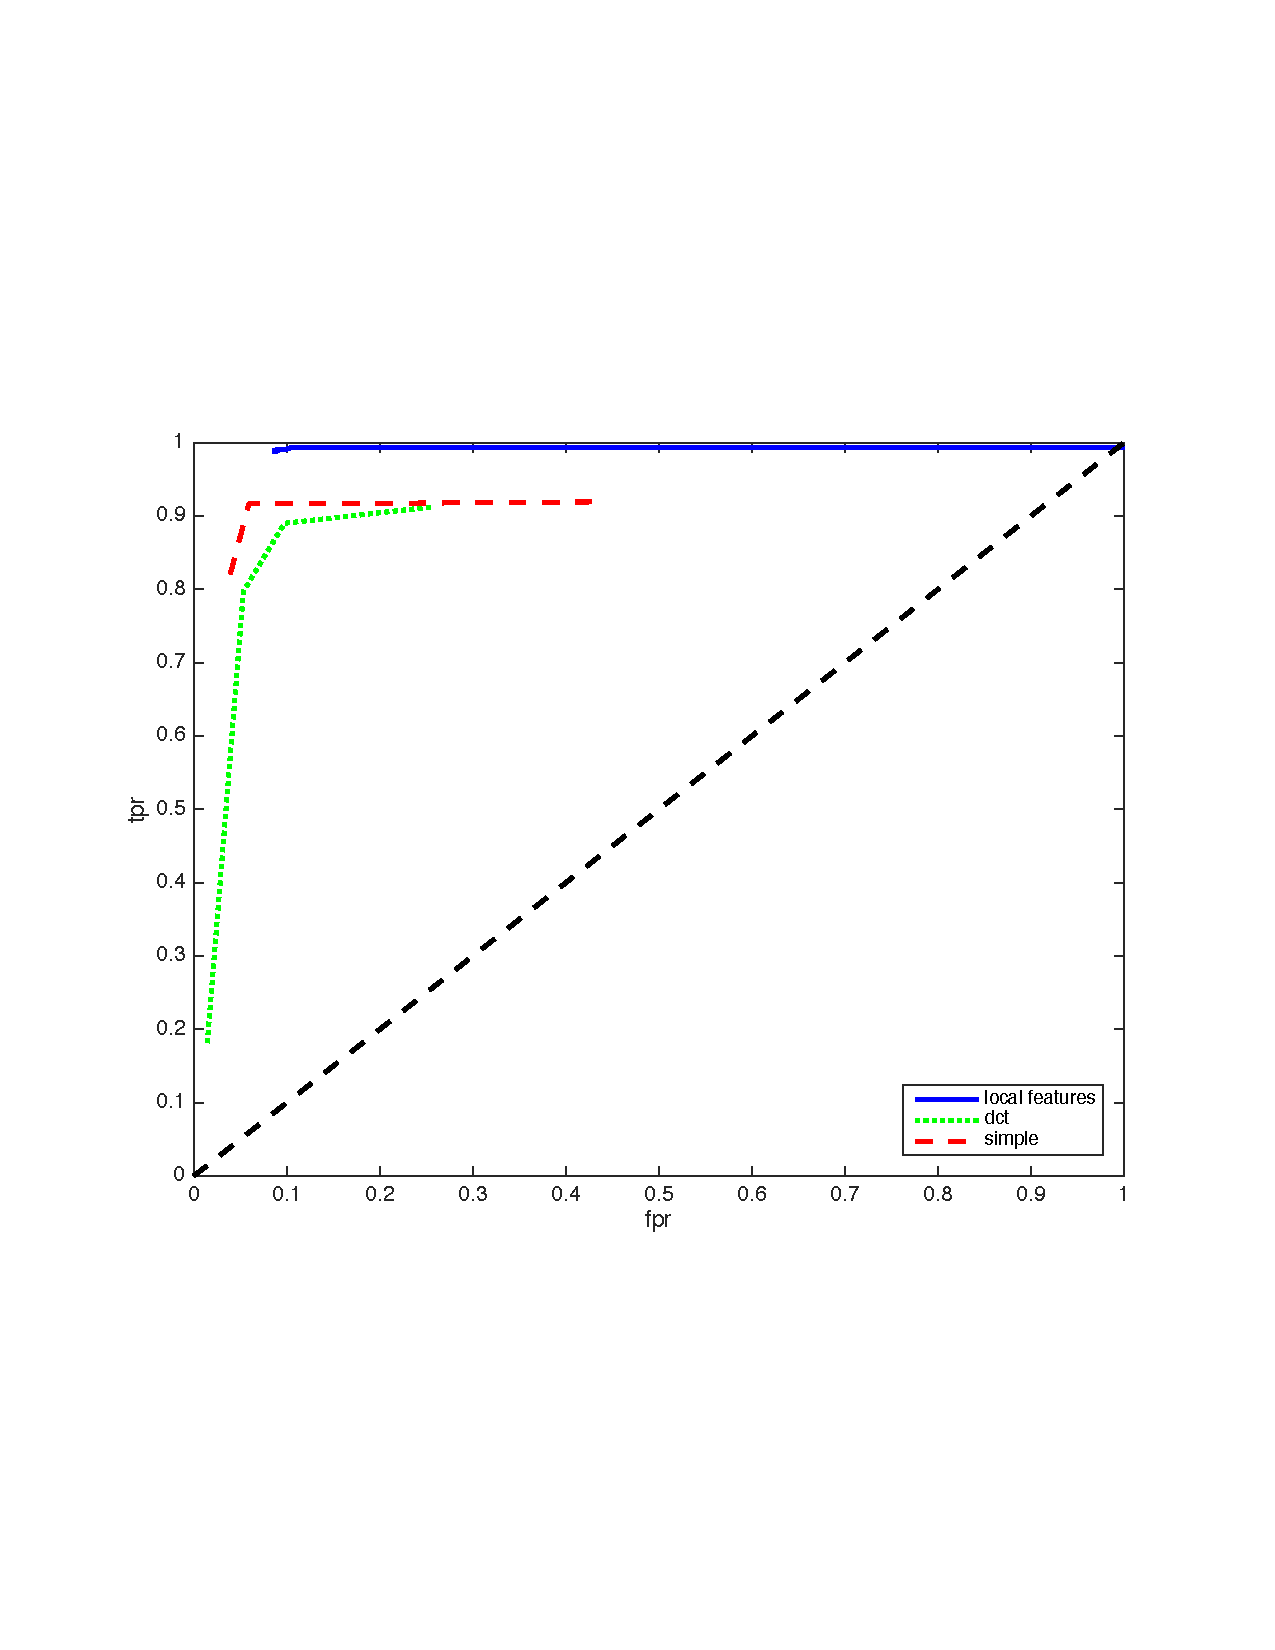
\includegraphics[width=\textwidth]{figures/thinglink_83scaleROC.pdf}
    \caption{ThingLink ROC}
    \label{83pr}
  \end{subfigure}
  %
  \begin{subfigure}[b]{0.49\textwidth}
    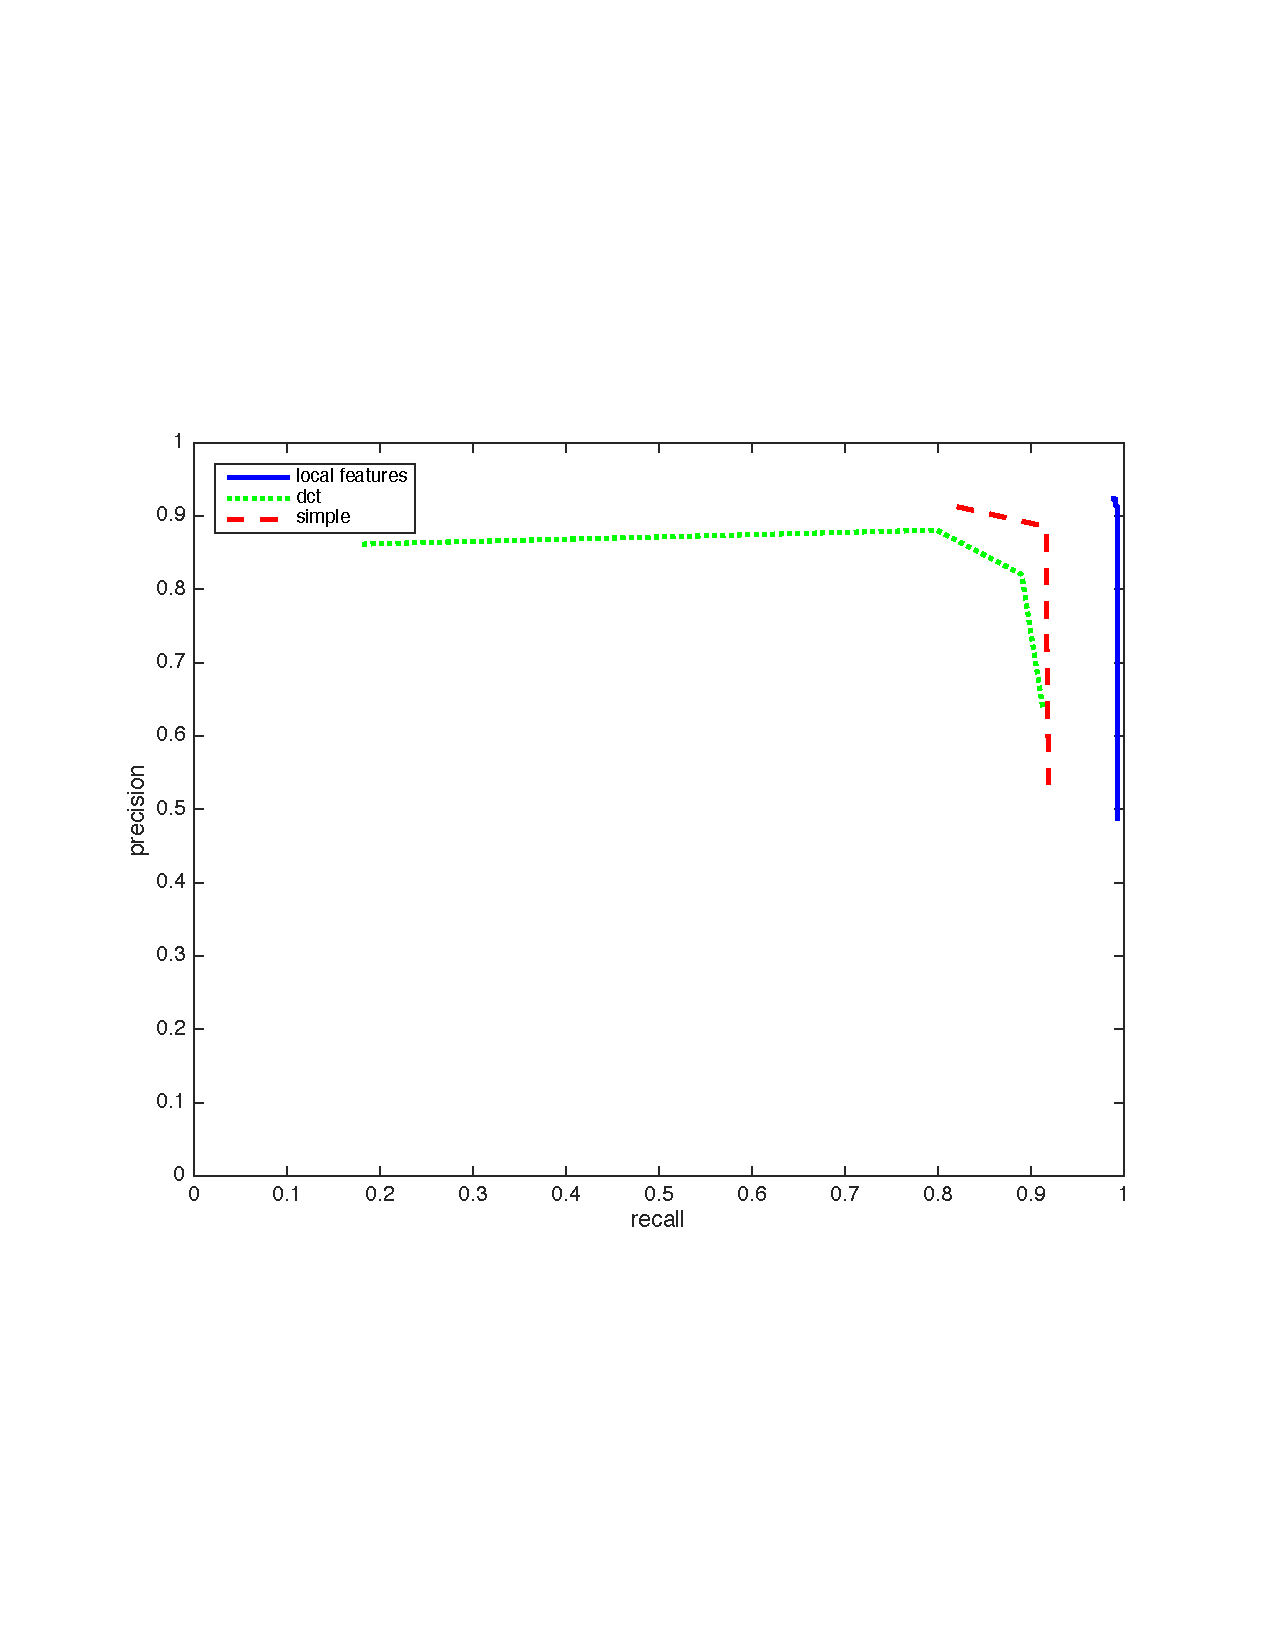
\includegraphics[width=\textwidth]{figures/thinglink_83scalePR.pdf}
    \caption{ThingLink PR}
    \label{83prthinglink}
  \end{subfigure}
  \caption{\emph{83\% scale near-duplicate query results.} See figure \ref{53label} for a detailed caption. \label{83label}}
  \end{center}
\end{figure}

\clearpage

\begin{figure}[htb]
  \begin{center}
  \begin{subfigure}[b]{0.49\textwidth}
    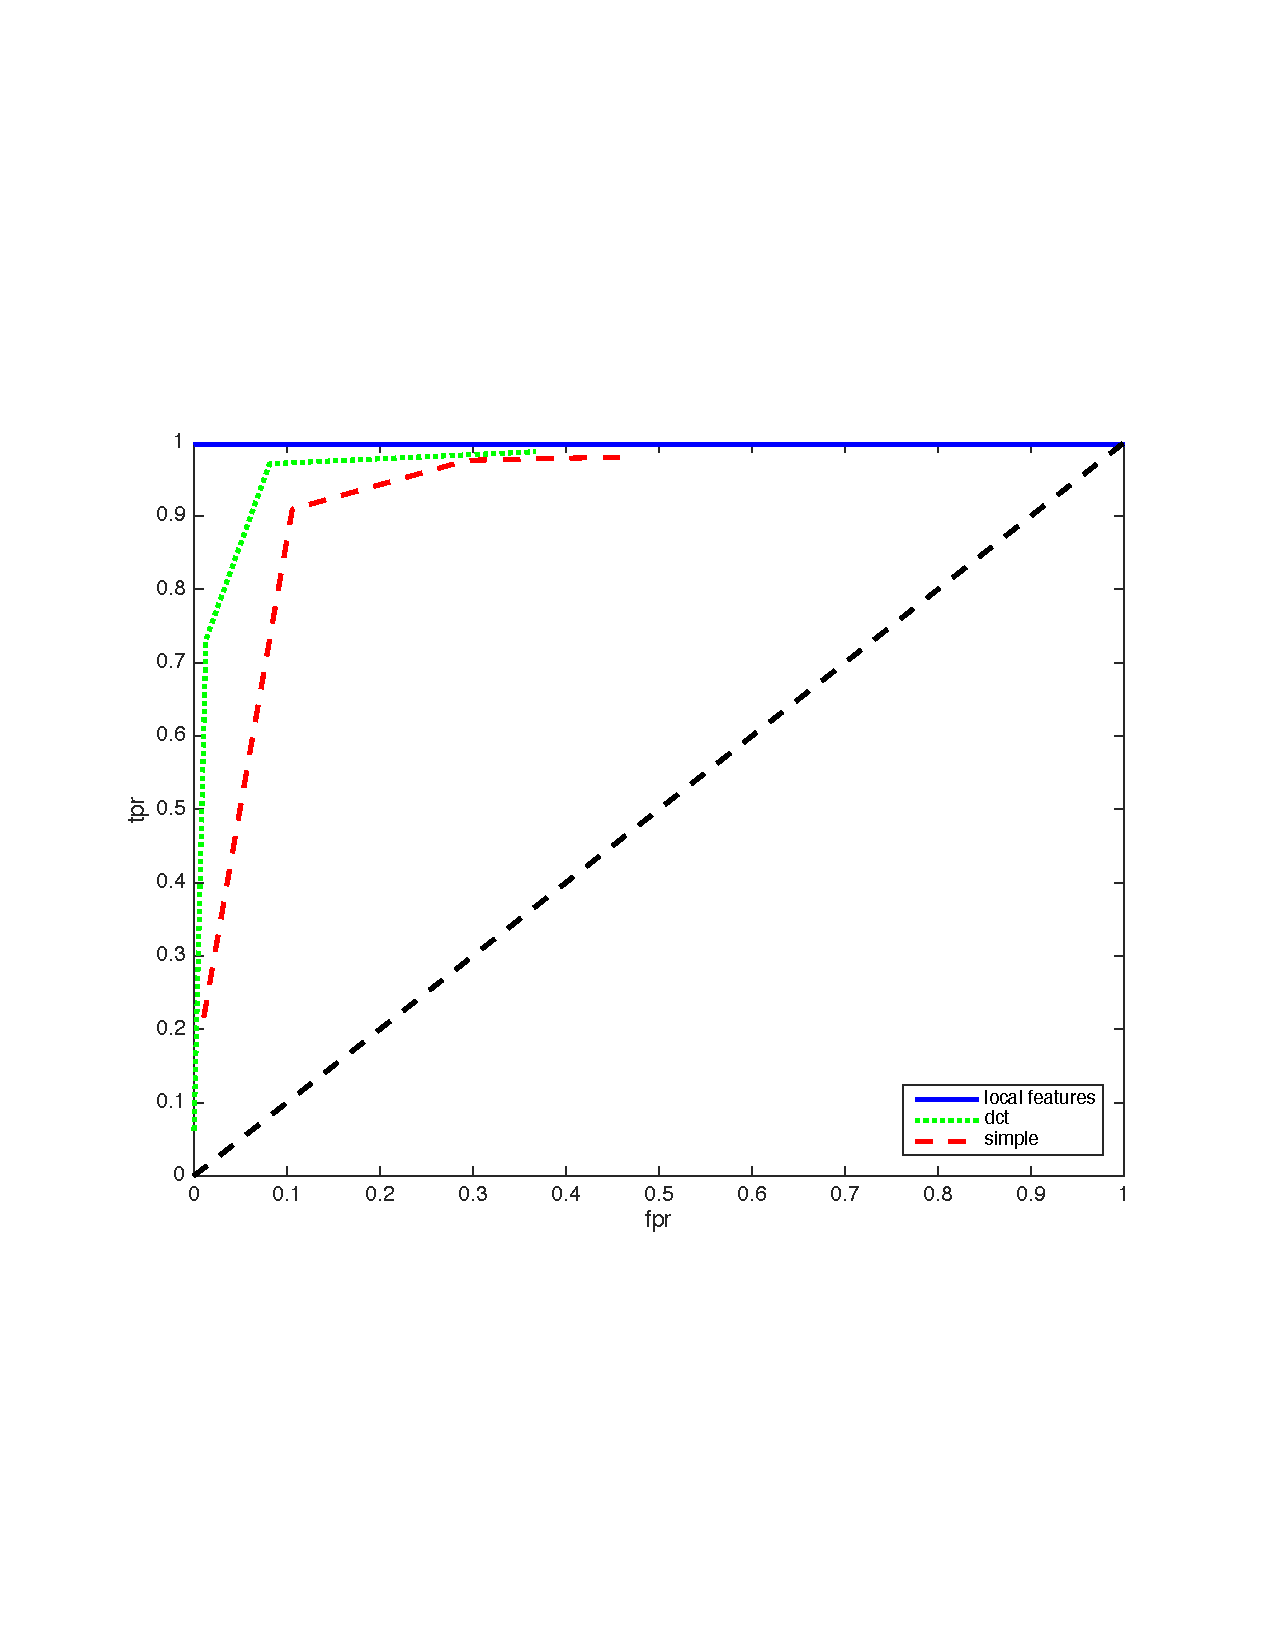
\includegraphics[width=\textwidth]{figures/Shave10pxROC.pdf}
    \caption{Paintings ROC}
    \label{Shaveroc}
  \end{subfigure}
  %
  \begin{subfigure}[b]{0.49\textwidth}
    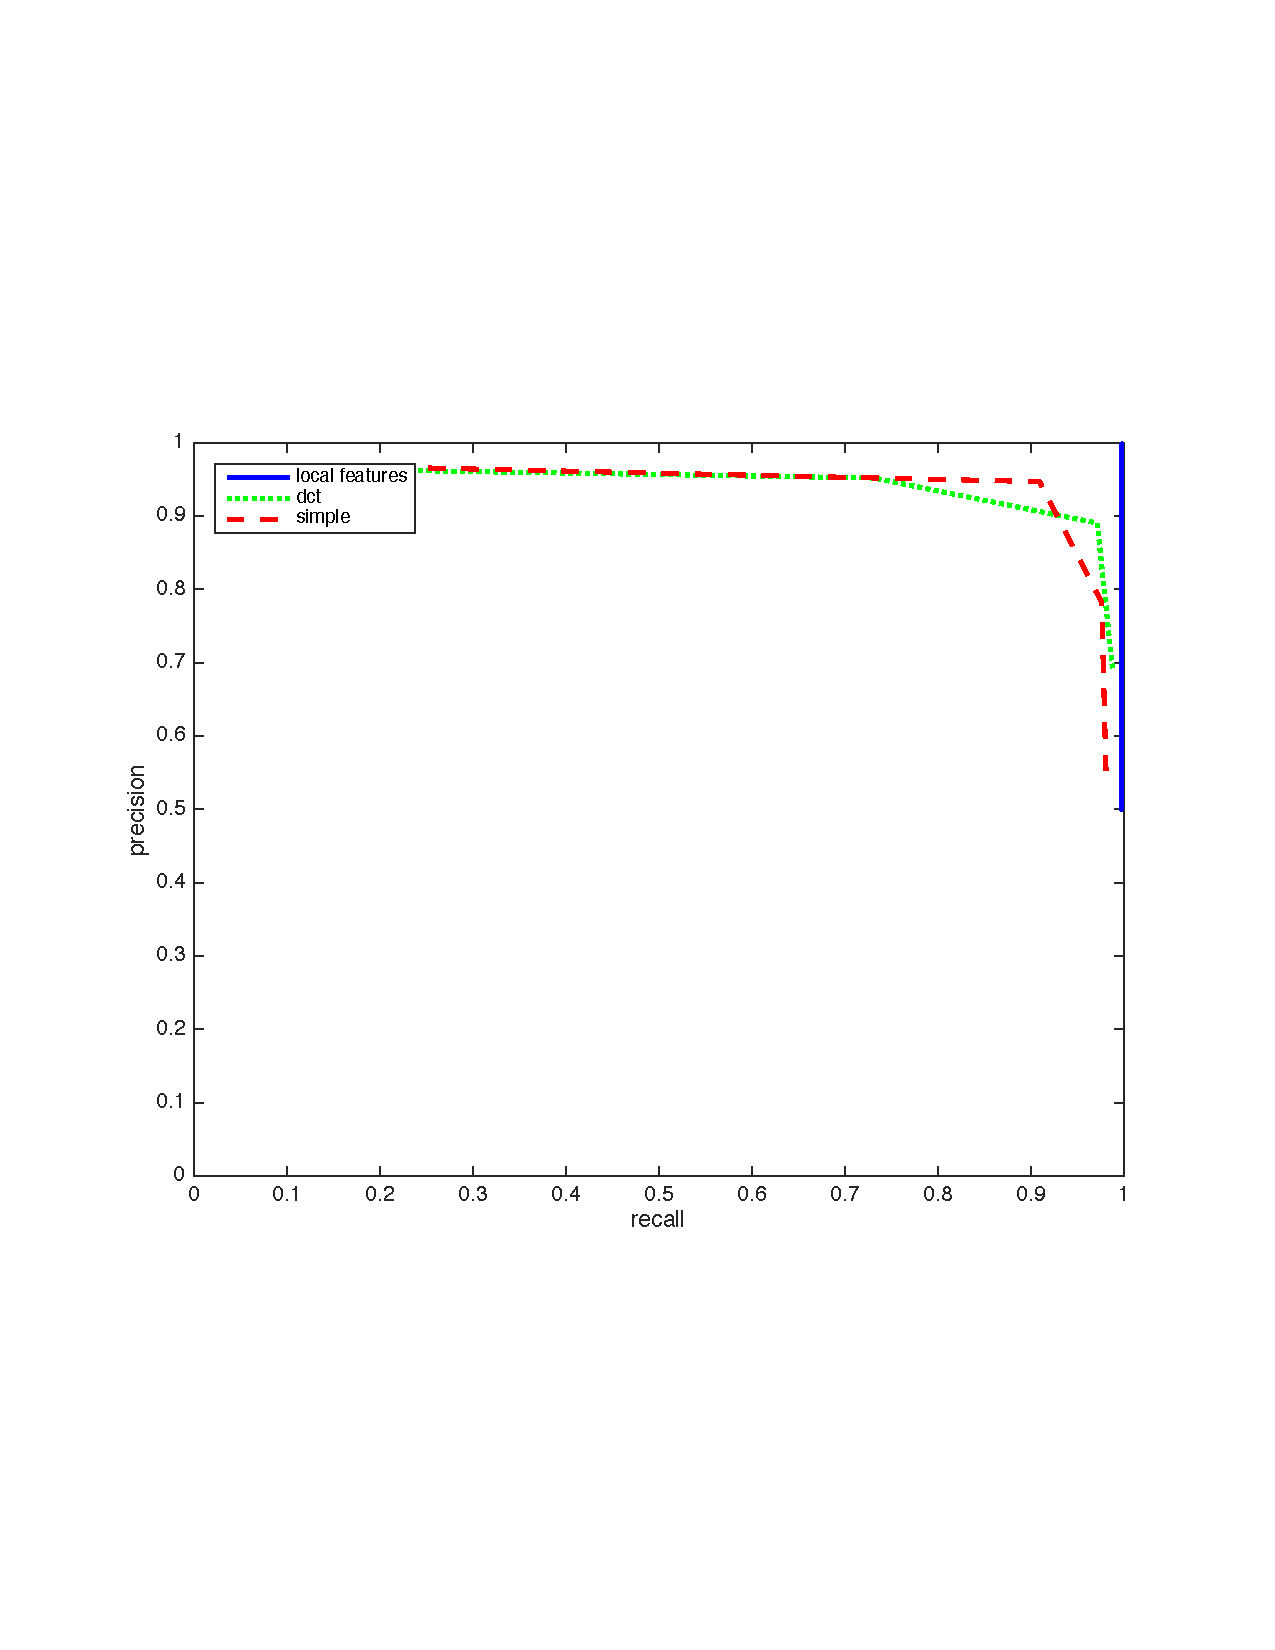
\includegraphics[width=\textwidth]{figures/Shave10pxPR.pdf}
    \caption{Paintings PR}
    \label{Shaverocthinglink}
  \end{subfigure}
  \begin{subfigure}[b]{0.49\textwidth}
    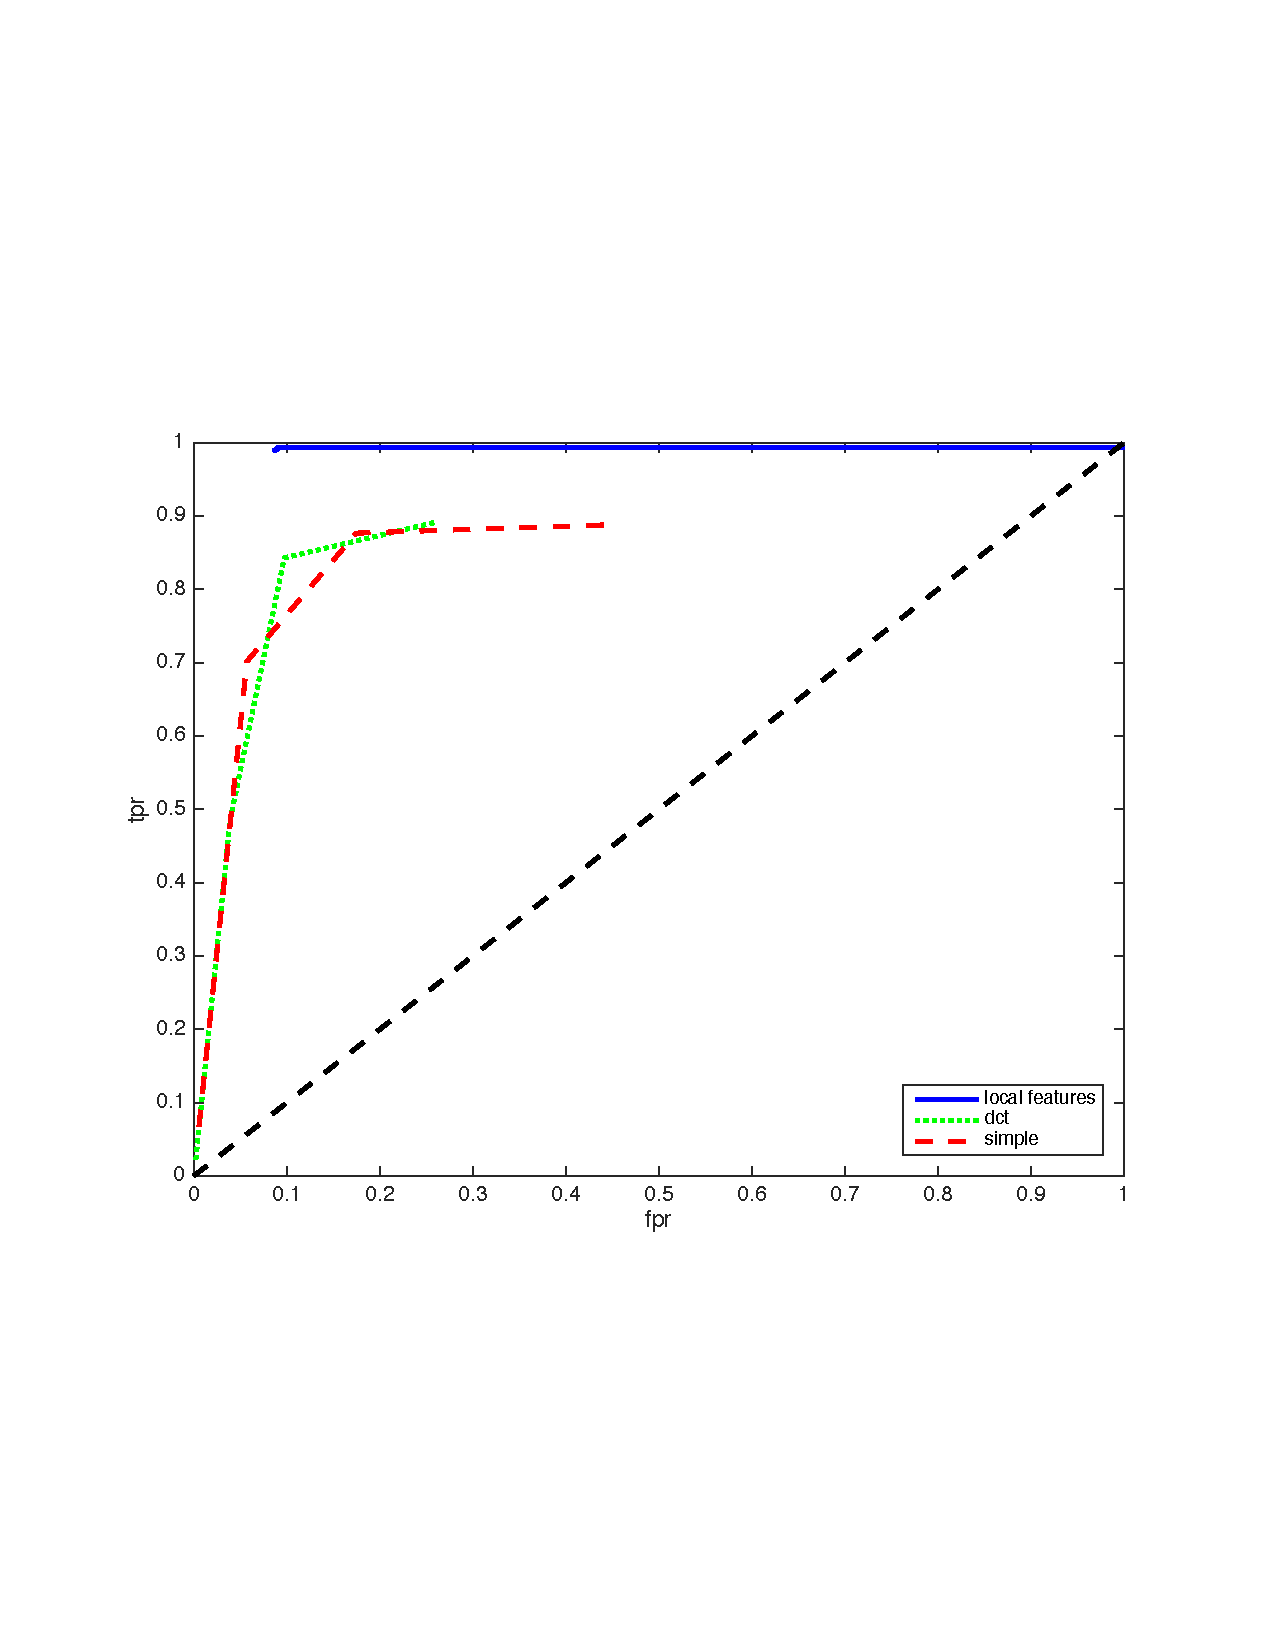
\includegraphics[width=\textwidth]{figures/thinglink_Shave10pxROC.pdf}
    \caption{ThingLink ROC}
    \label{Shavepr}
  \end{subfigure}
  %
  \begin{subfigure}[b]{0.49\textwidth}
    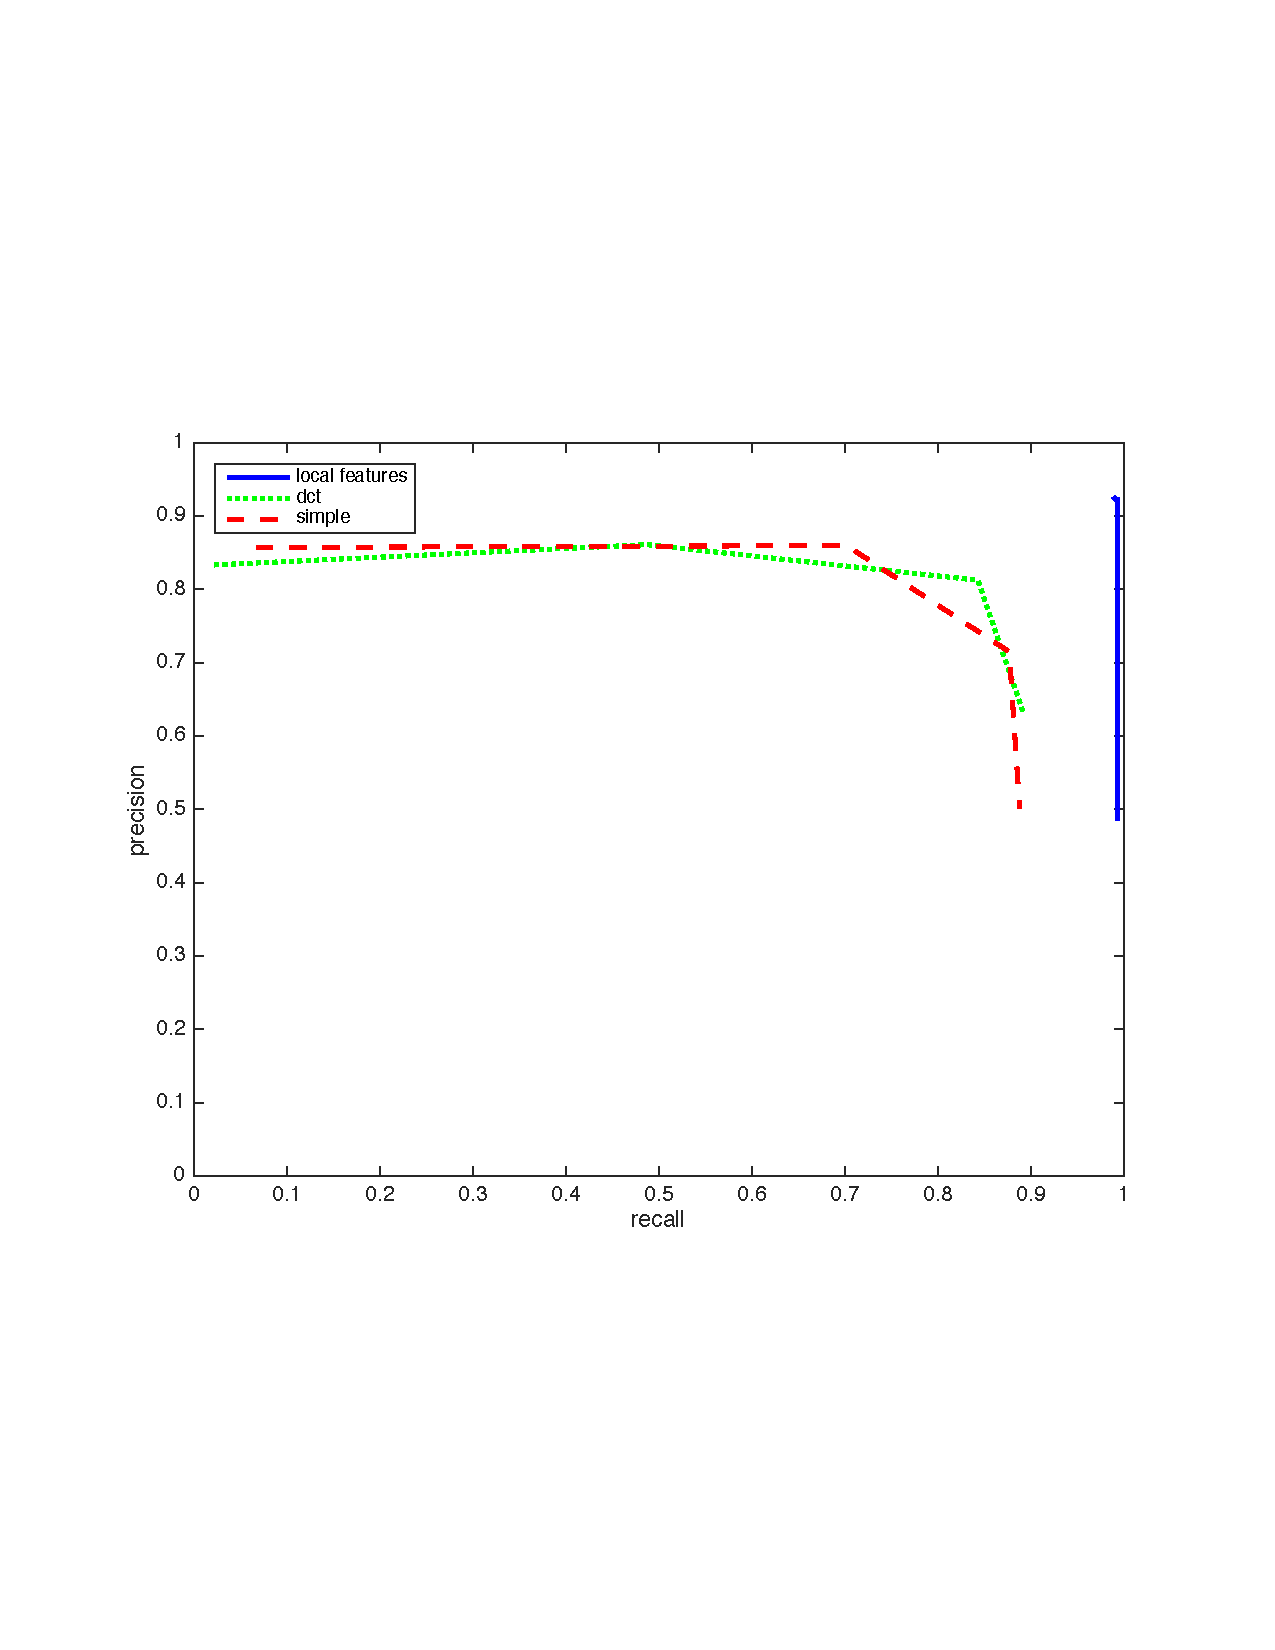
\includegraphics[width=\textwidth]{figures/thinglink_Shave10pxPR.pdf}
    \caption{ThingLink PR}
    \label{Shaveprthinglink}
  \end{subfigure}
  \caption{\emph{Shave 10px near-duplicate query results.} See figure \ref{53label} for a detailed caption.\label{shavelabel}}
  \end{center}
\end{figure}


\begin{figure}[htb]
  \begin{center}
  \begin{subfigure}[b]{0.49\textwidth}
    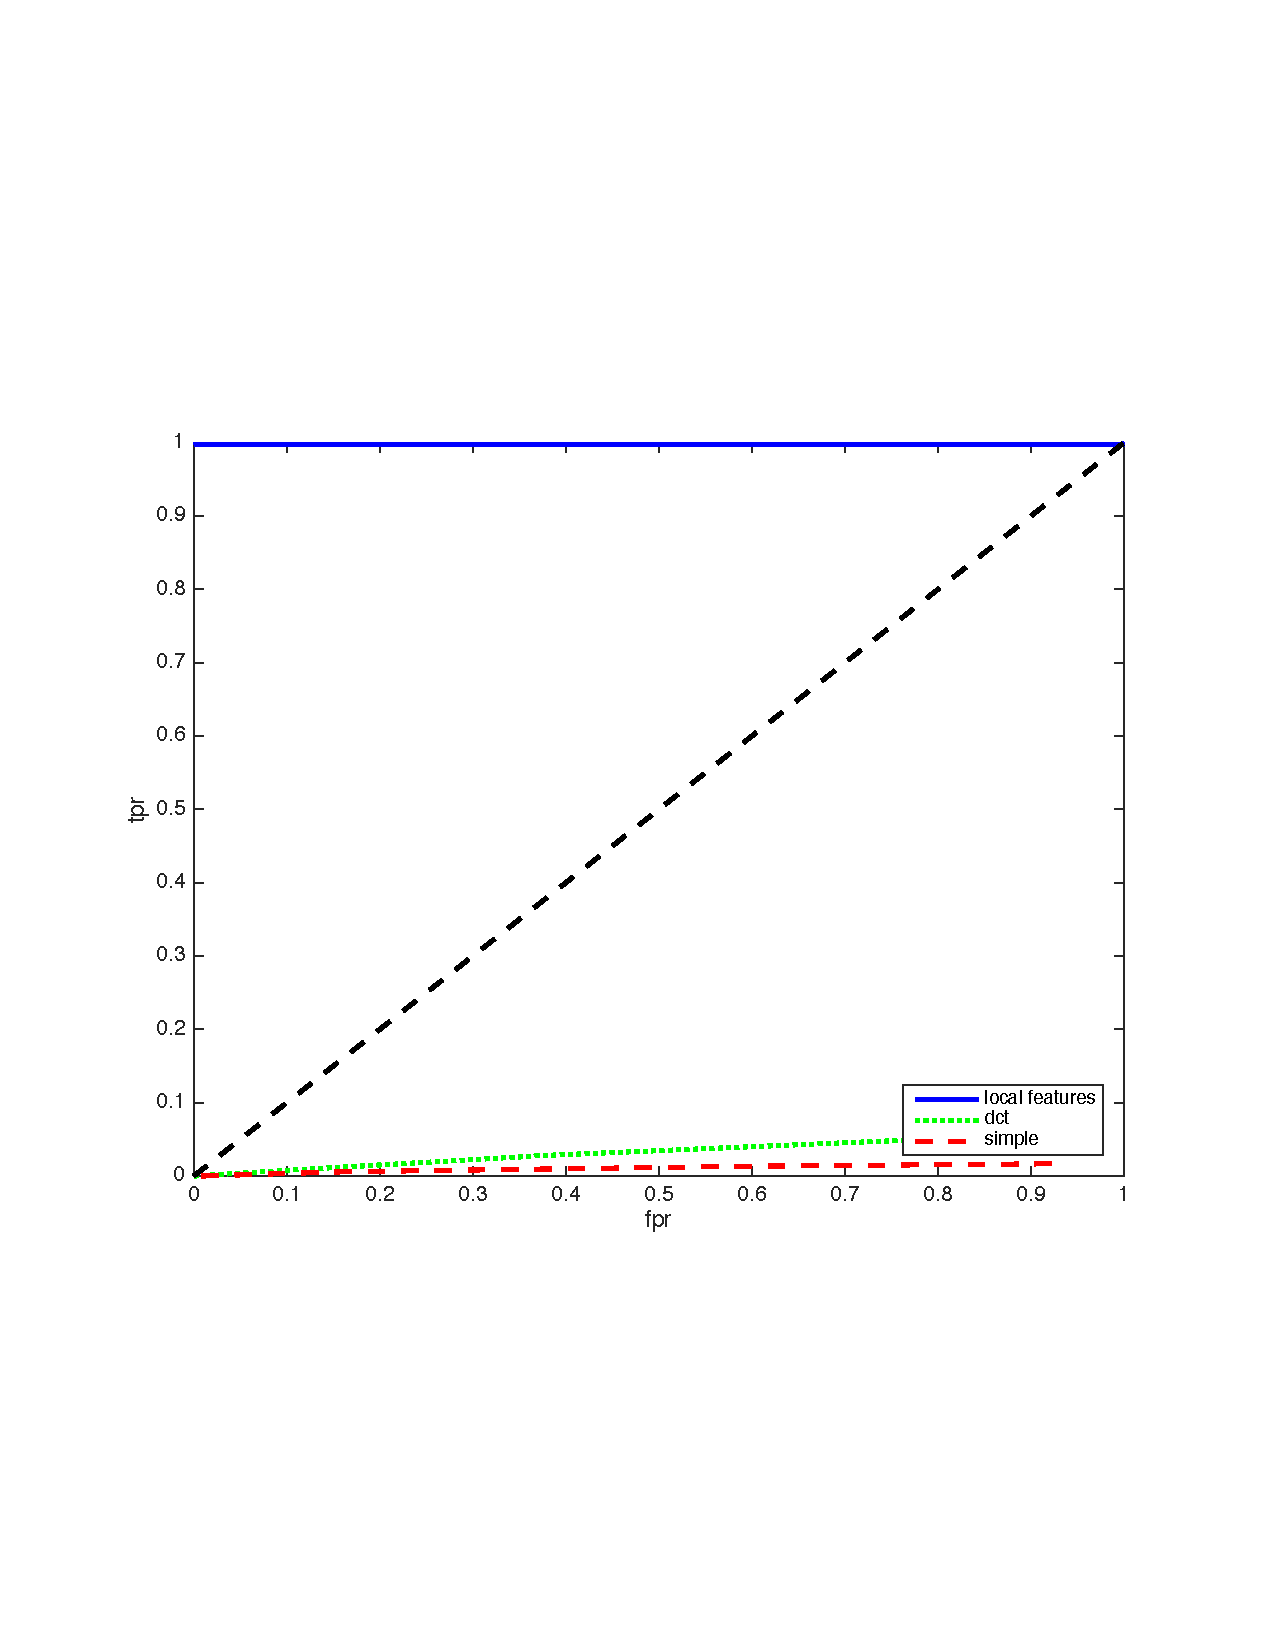
\includegraphics[width=\textwidth]{figures/Border10ROC.pdf}
    \caption{Paintings ROC}
    \label{Borderroc}
  \end{subfigure}
  %
  \begin{subfigure}[b]{0.49\textwidth}
    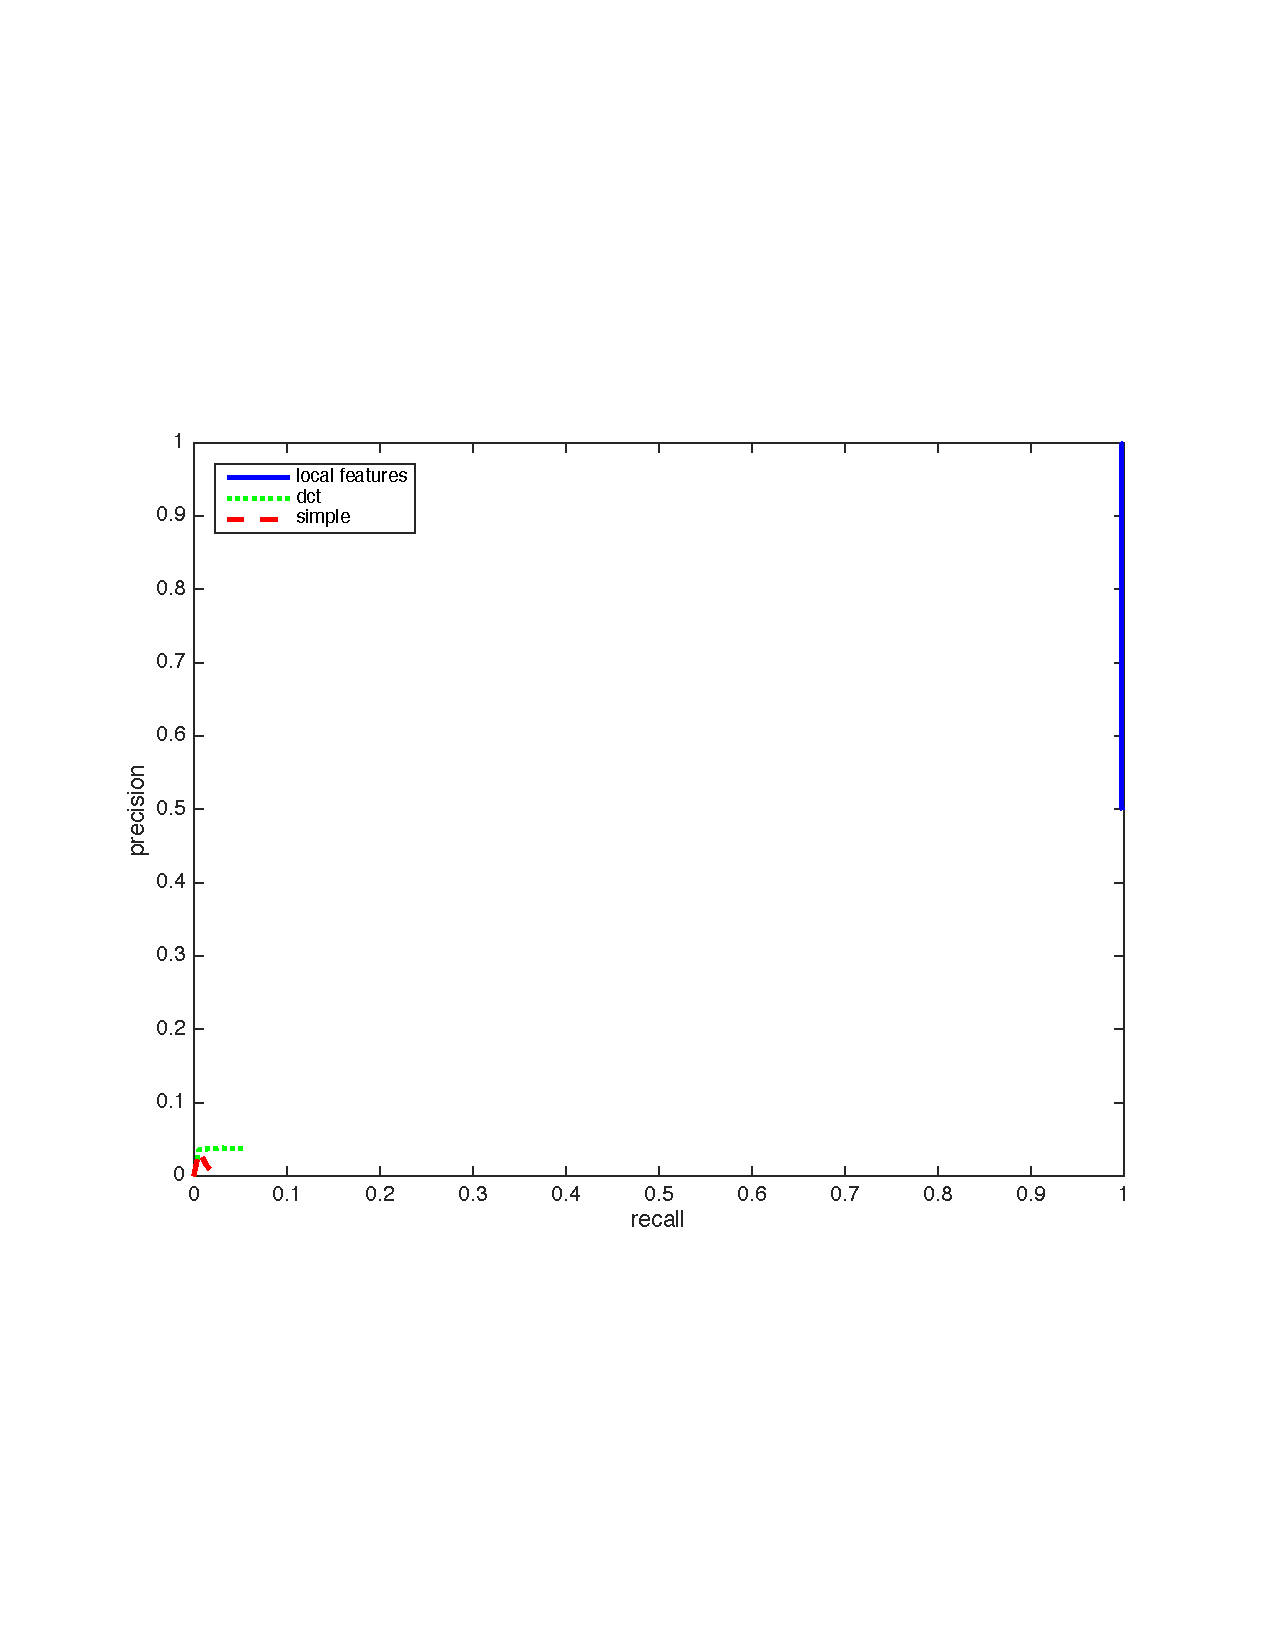
\includegraphics[width=\textwidth]{figures/Border10PR.pdf}
    \caption{Paintings PR}
    \label{Borderrocthinglink}
  \end{subfigure}
  \begin{subfigure}[b]{0.49\textwidth}
    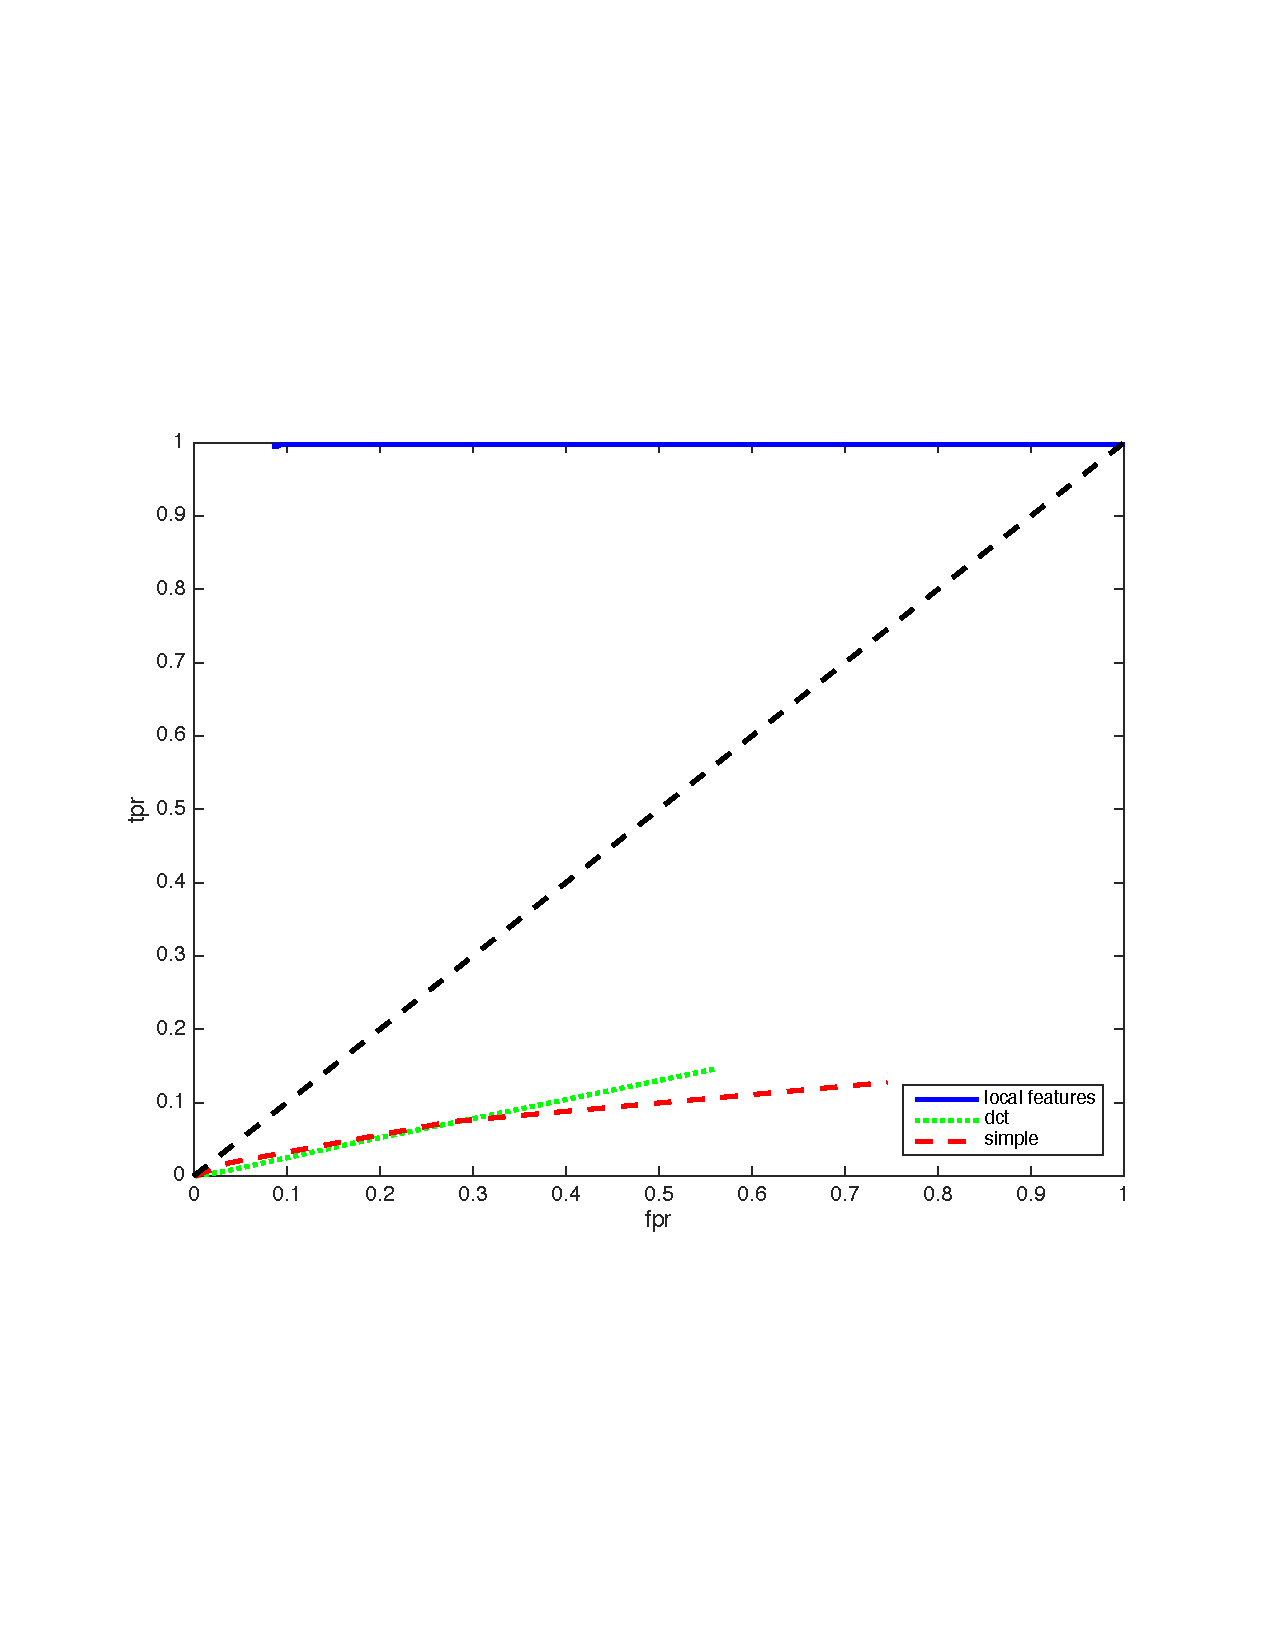
\includegraphics[width=\textwidth]{figures/thinglink_Border10ROC.pdf}
    \caption{ThingLink ROC}
    \label{Borderpr}
  \end{subfigure}
  %
  \begin{subfigure}[b]{0.49\textwidth}
    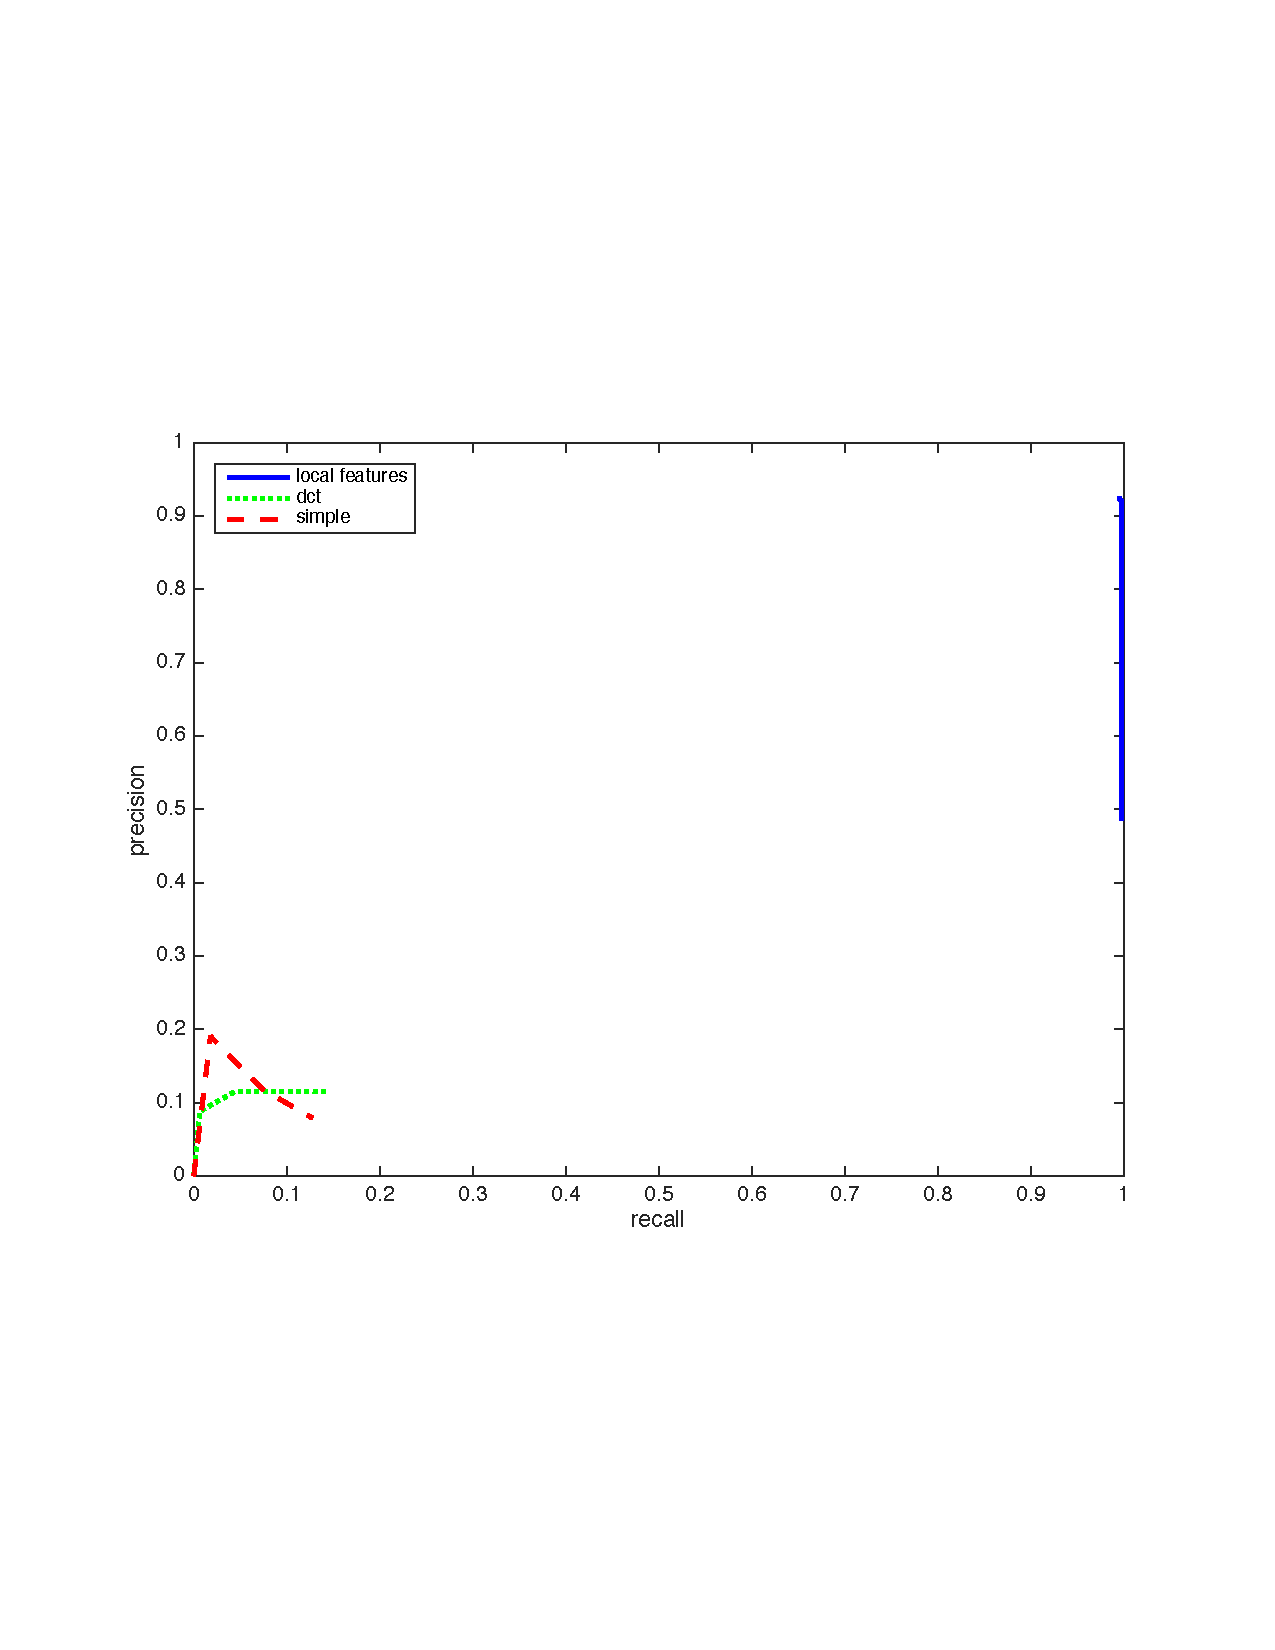
\includegraphics[width=\textwidth]{figures/thinglink_Border10PR.pdf}
    \caption{ThingLink PR}
    \label{Borderprthinglink}
  \end{subfigure}
  \caption{\emph{Border 10\% near-duplicate query results.} See figure \ref{53label} for a detailed caption. \label{borderlabel}}
  \end{center}
\end{figure}



\begin{figure}[htb]
  \begin{center}
  \begin{subfigure}[b]{0.49\textwidth}
    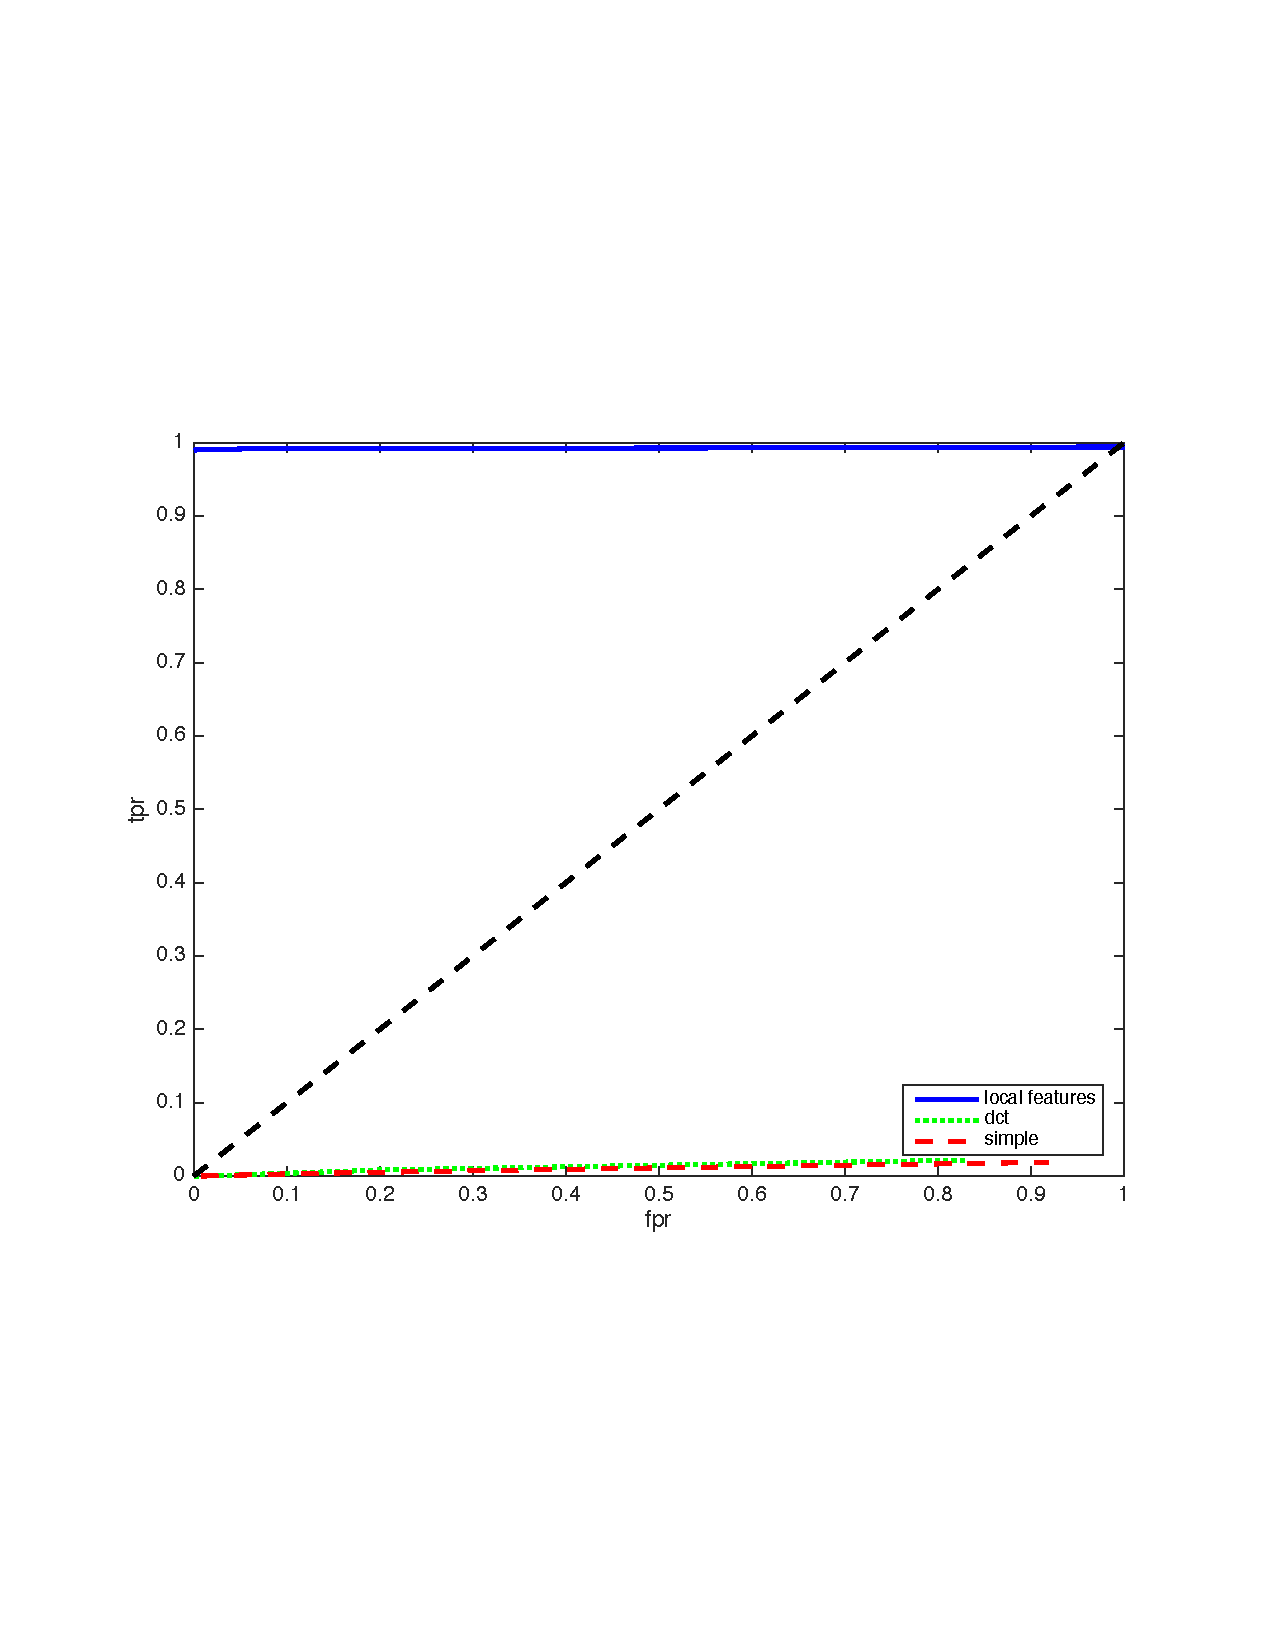
\includegraphics[width=\textwidth]{figures/Rotate10ROC.pdf}
    \caption{Paintings ROC}
    \label{Rotateroc}
  \end{subfigure}
  %
  \begin{subfigure}[b]{0.49\textwidth}
    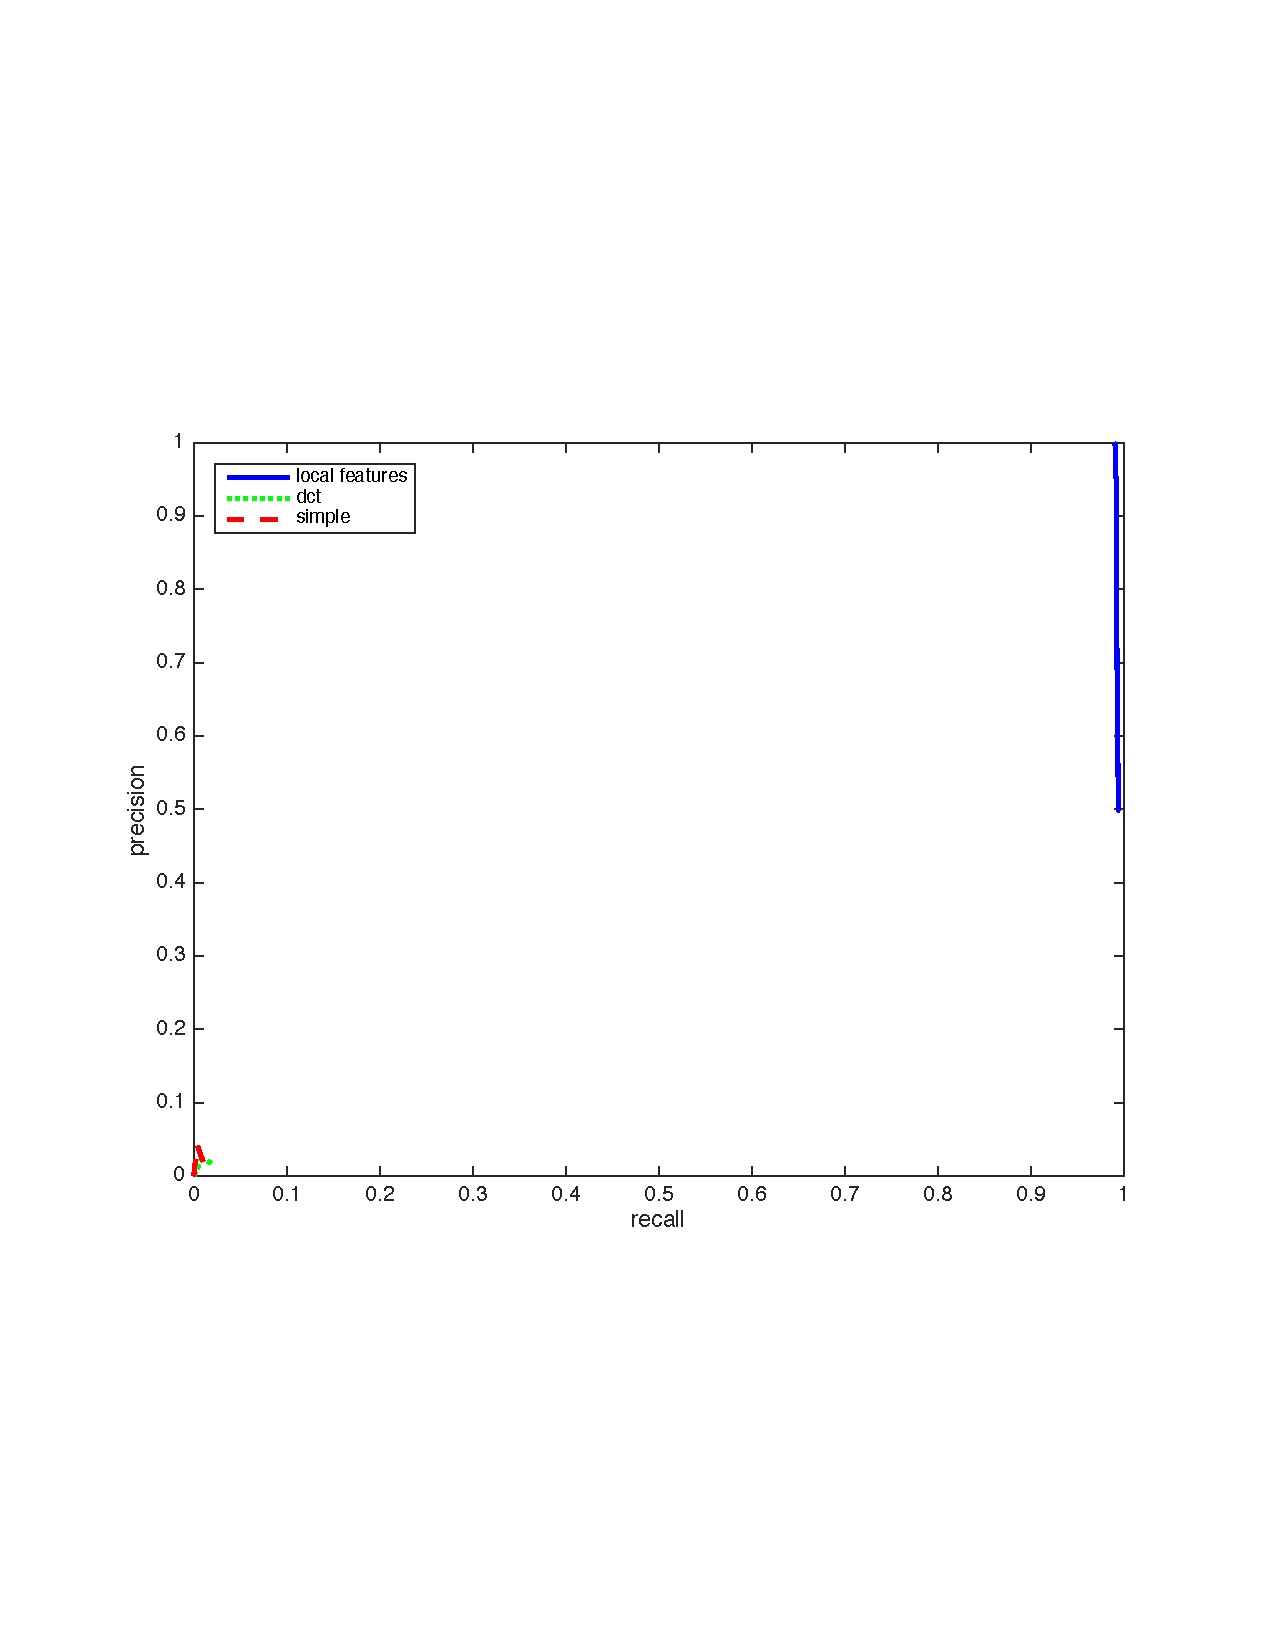
\includegraphics[width=\textwidth]{figures/Rotate10PR.pdf}
    \caption{Paintings PR}
    \label{Rotaterocthinglink}
  \end{subfigure}
  \begin{subfigure}[b]{0.49\textwidth}
    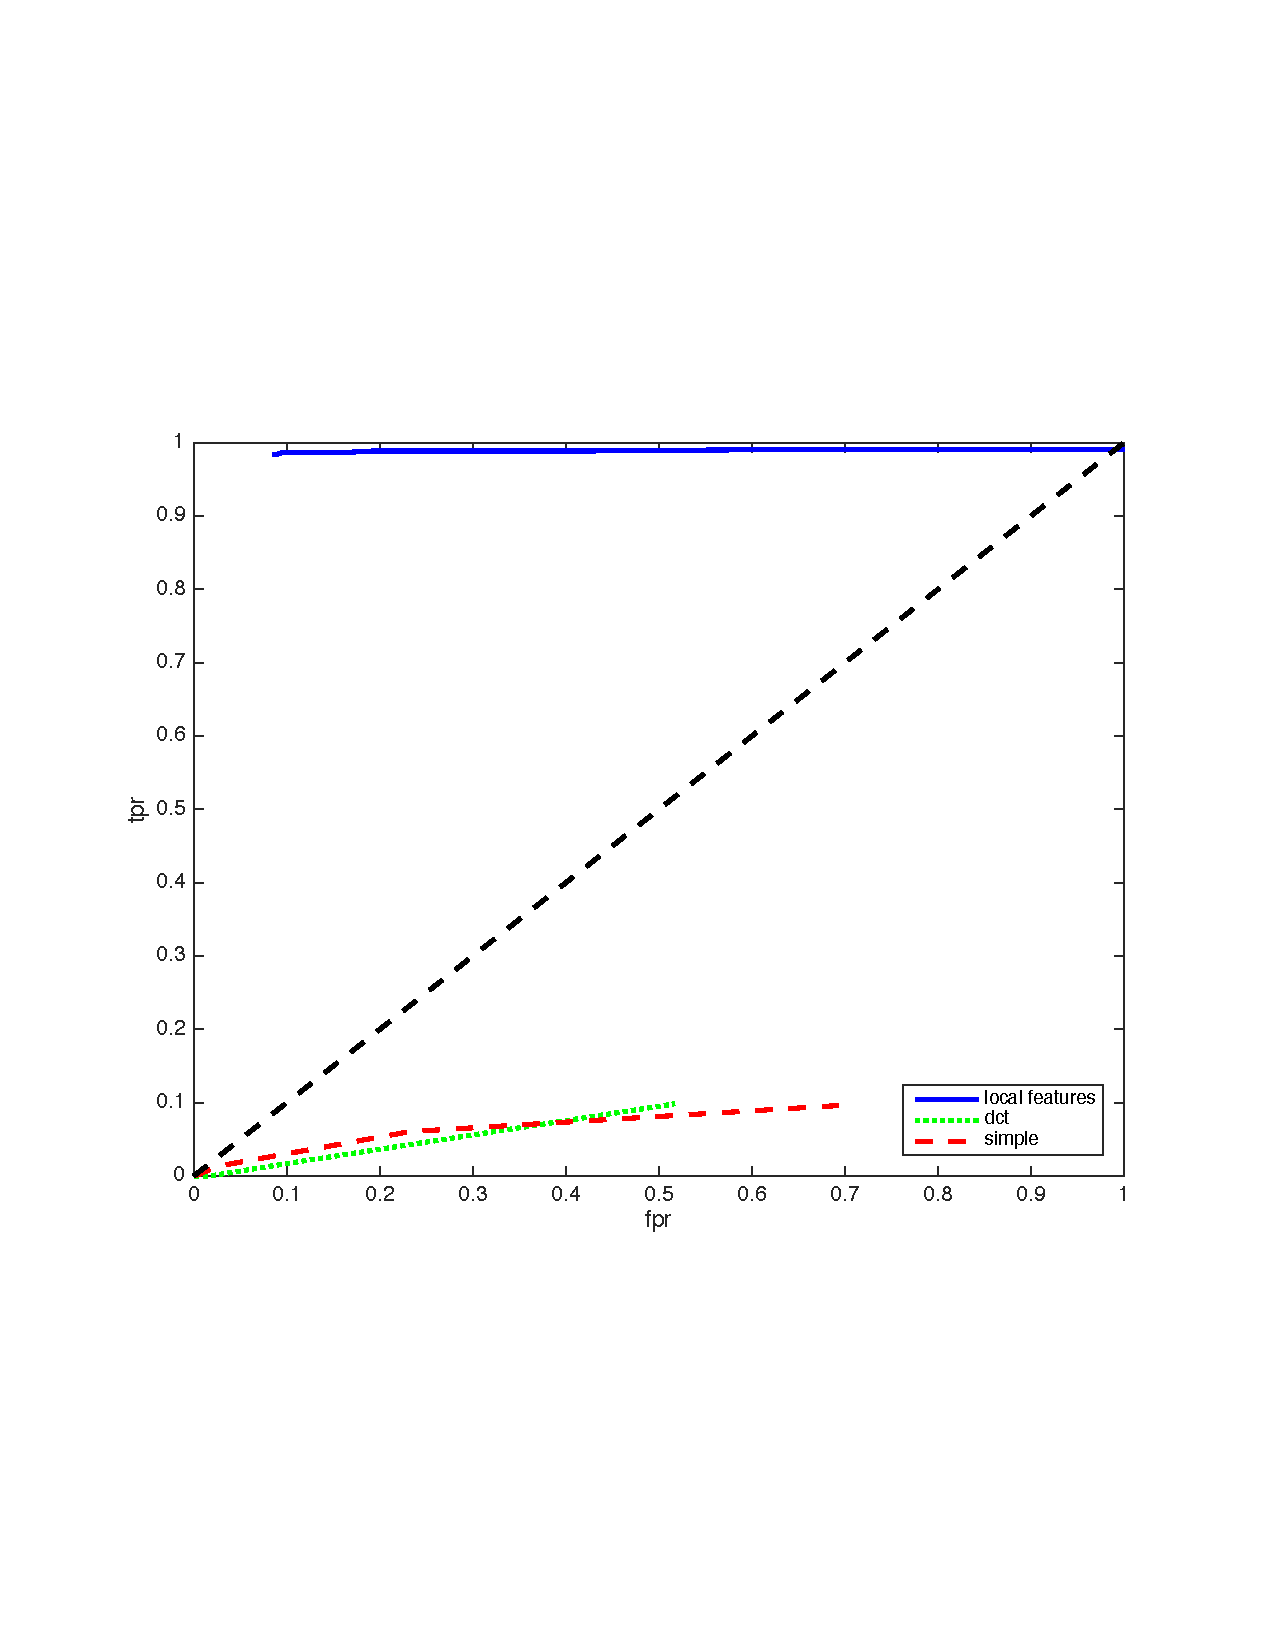
\includegraphics[width=\textwidth]{figures/thinglink_Rotate10ROC.pdf}
    \caption{ThingLink ROC}
    \label{Rotatepr}
  \end{subfigure}
  %
  \begin{subfigure}[b]{0.49\textwidth}
    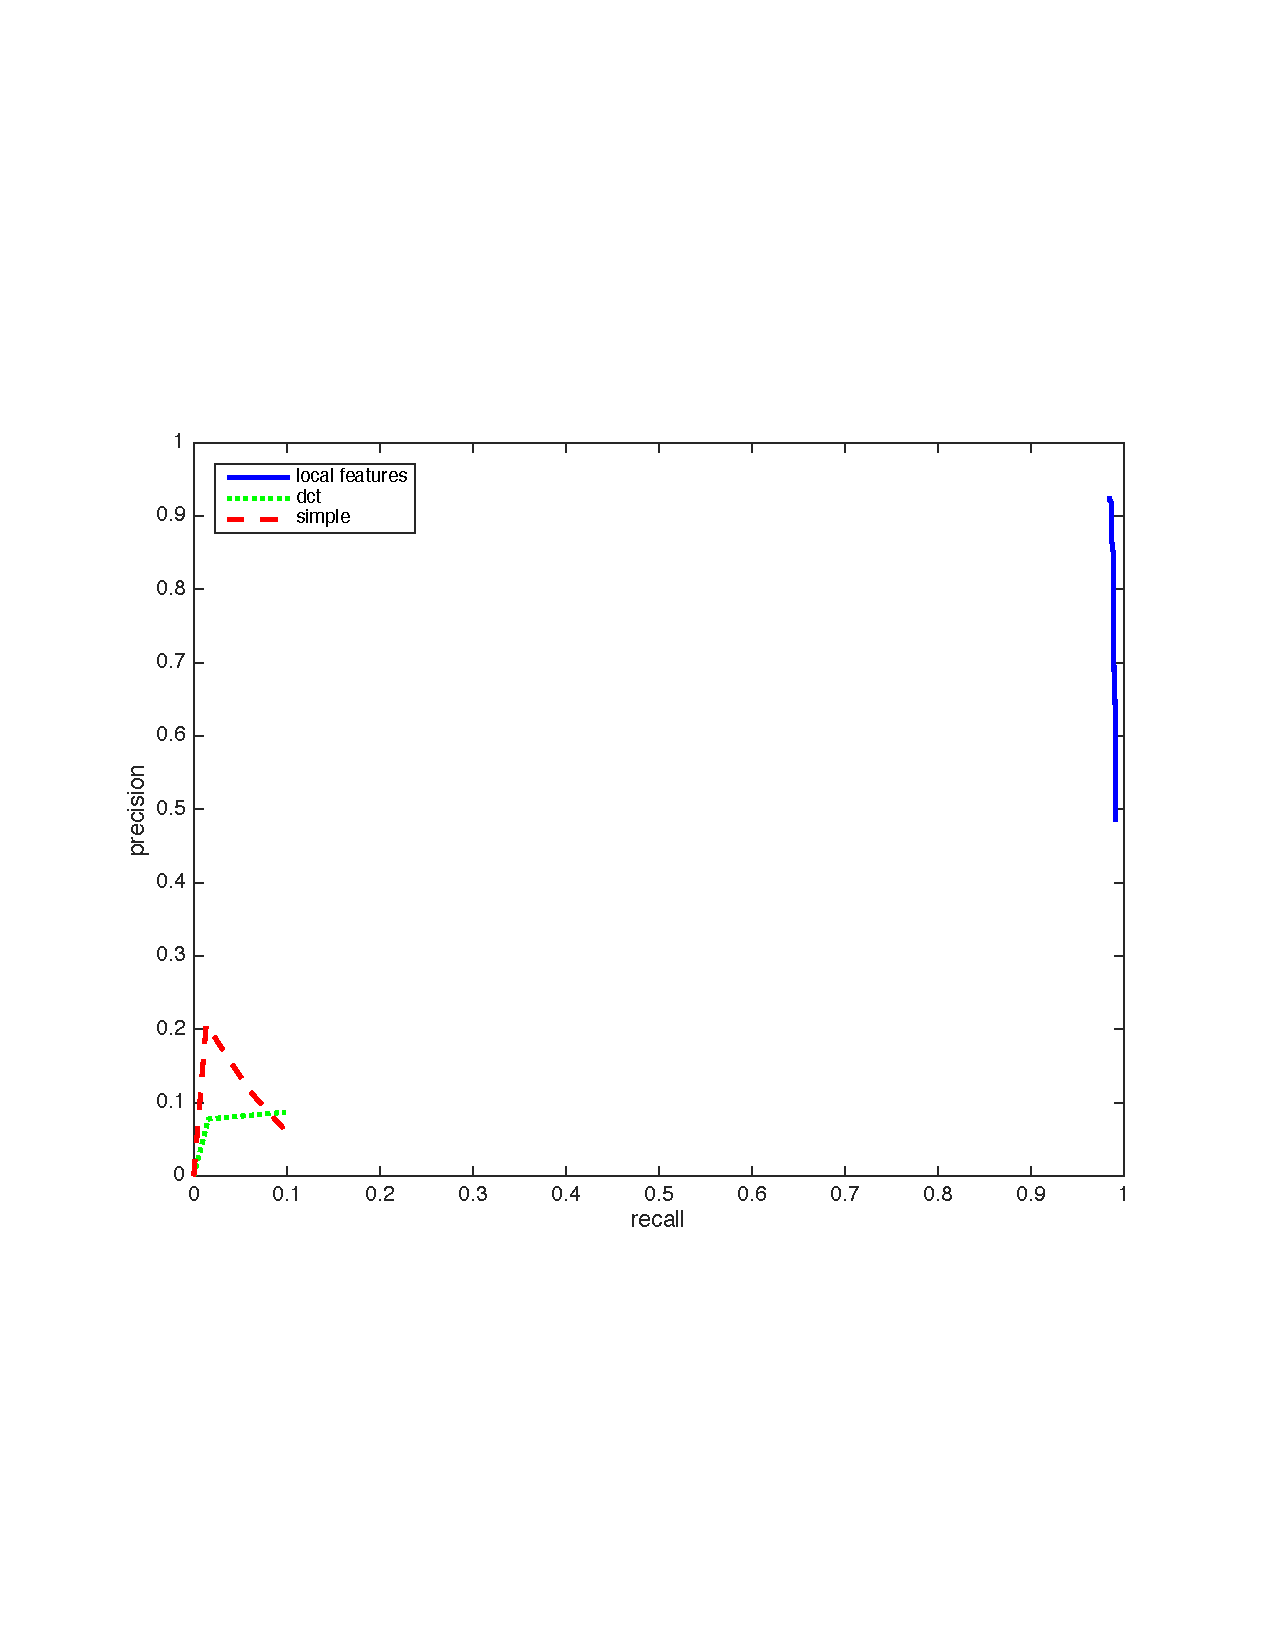
\includegraphics[width=\textwidth]{figures/thinglink_Rotate10PR.pdf}
    \caption{ThingLink PR}
    \label{Rotateprthinglink}
  \end{subfigure}
  \caption{\emph{Rotate 10\% near-duplicate query results.} See figure \ref{53label} for a detailed caption.\label{rotatelabel}}
  \end{center}
\end{figure}

\begin{figure}[htb]
  \begin{center}
  \begin{subfigure}[b]{0.49\textwidth}
    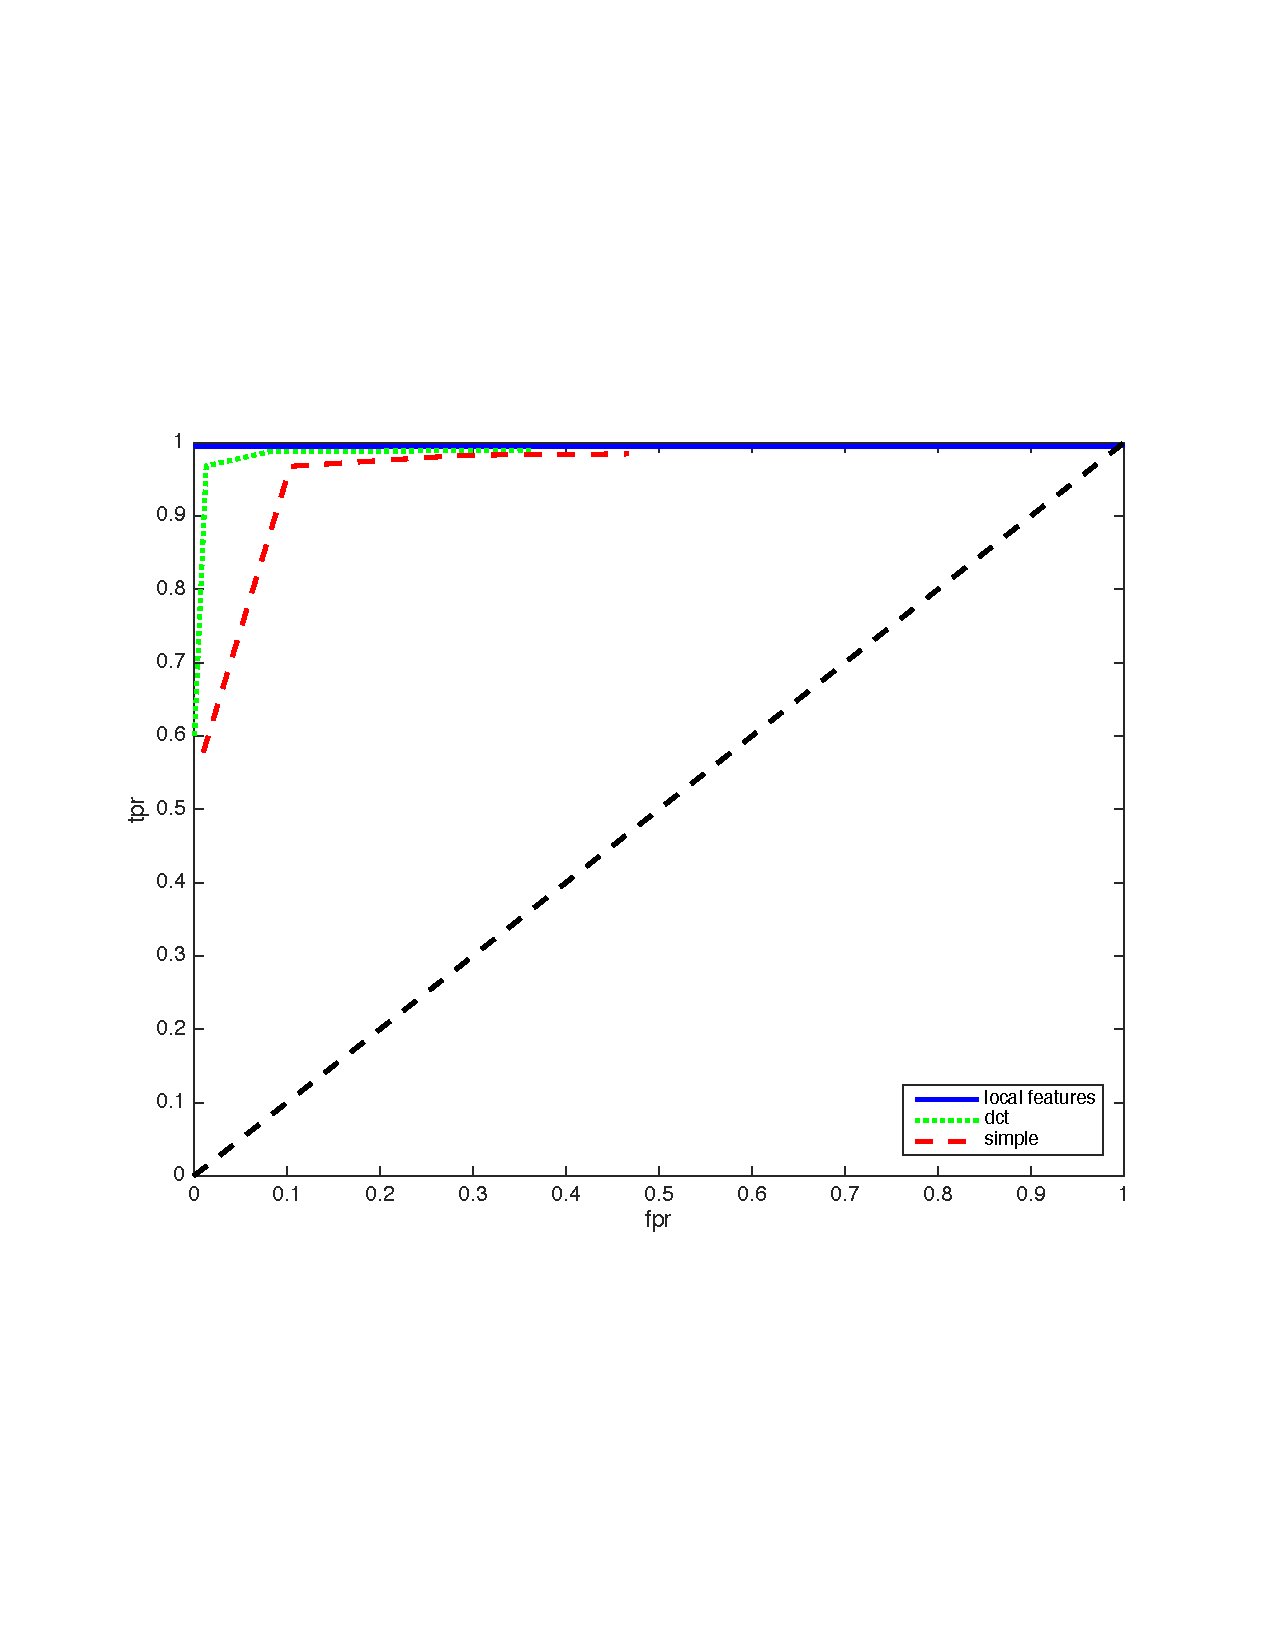
\includegraphics[width=\textwidth]{figures/NormalizehistogramROC.pdf}
    \caption{Paintings ROC}
    \label{Normalizeroc}
  \end{subfigure}
  %
  \begin{subfigure}[b]{0.49\textwidth}
    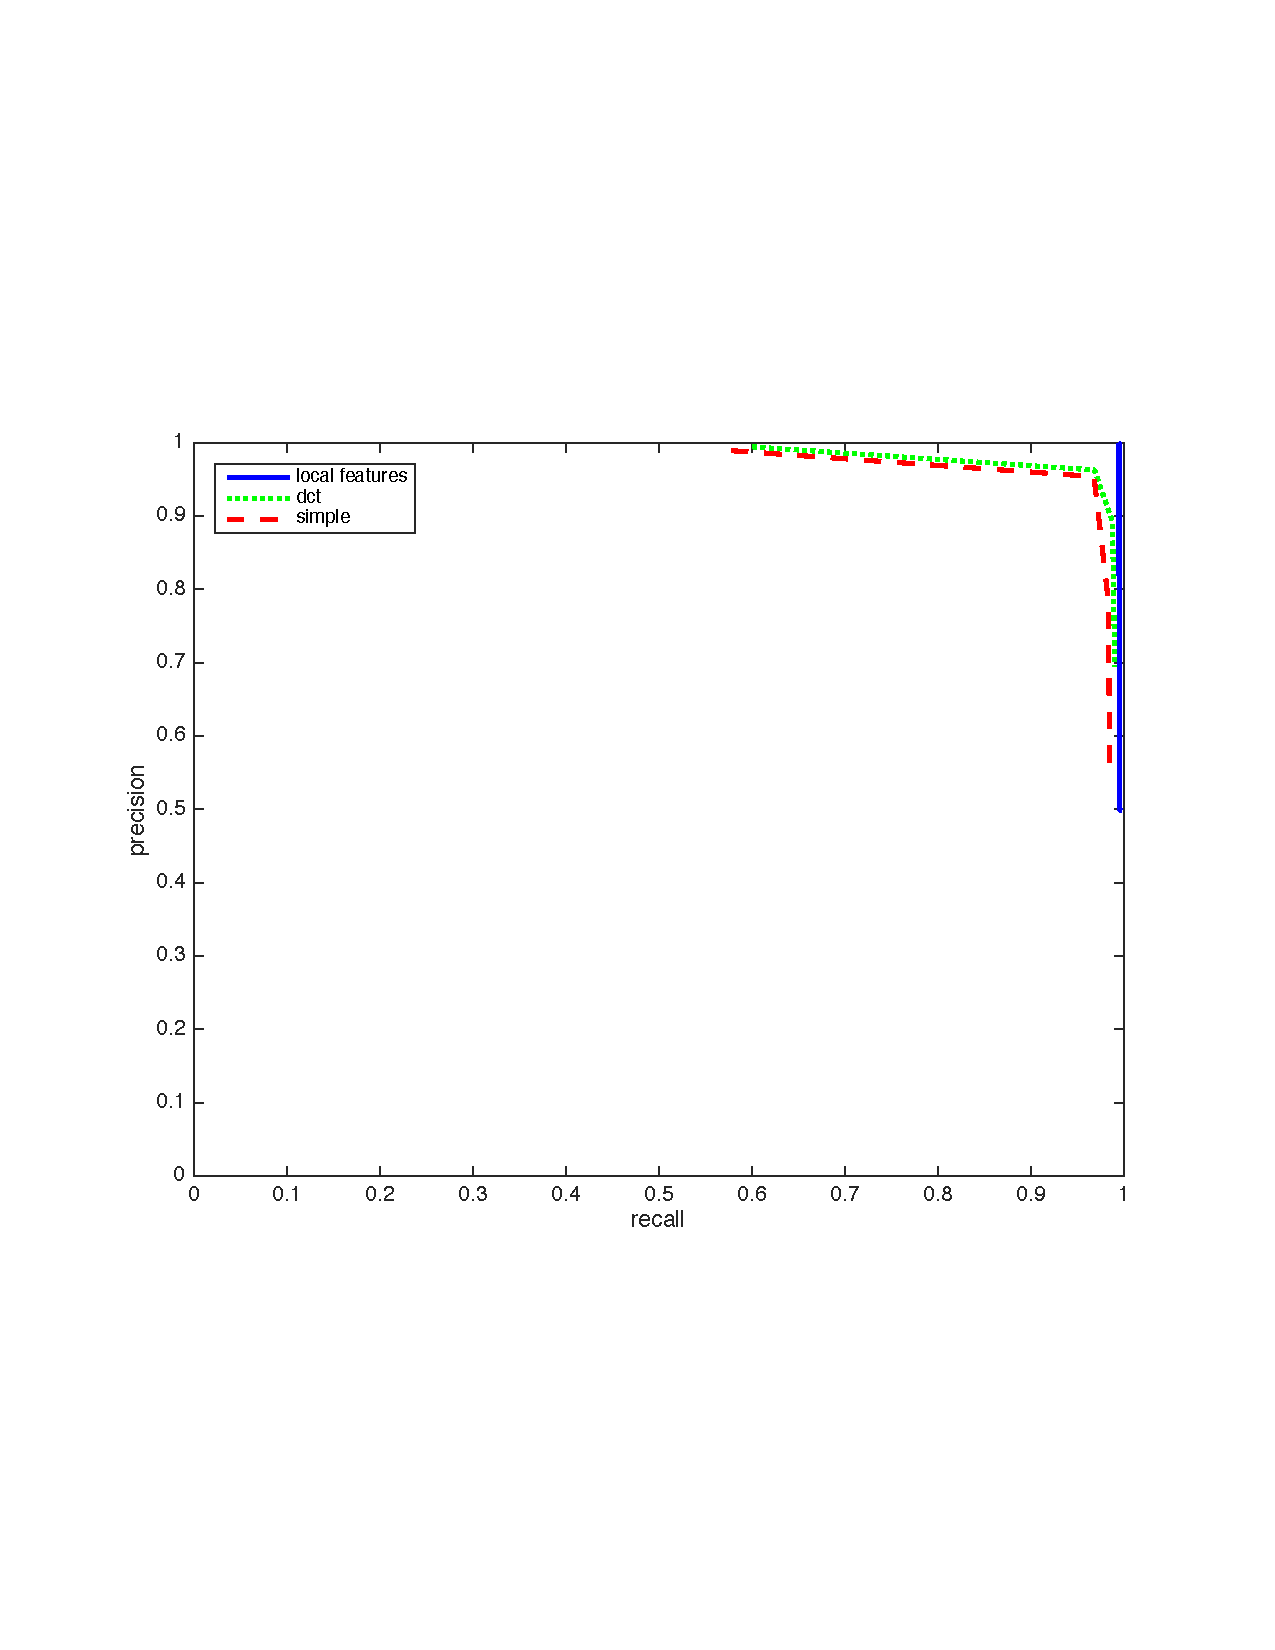
\includegraphics[width=\textwidth]{figures/NormalizehistogramPR.pdf}
    \caption{Paintings PR}
    \label{Normalizerocthinglink}
  \end{subfigure}
  \begin{subfigure}[b]{0.49\textwidth}
    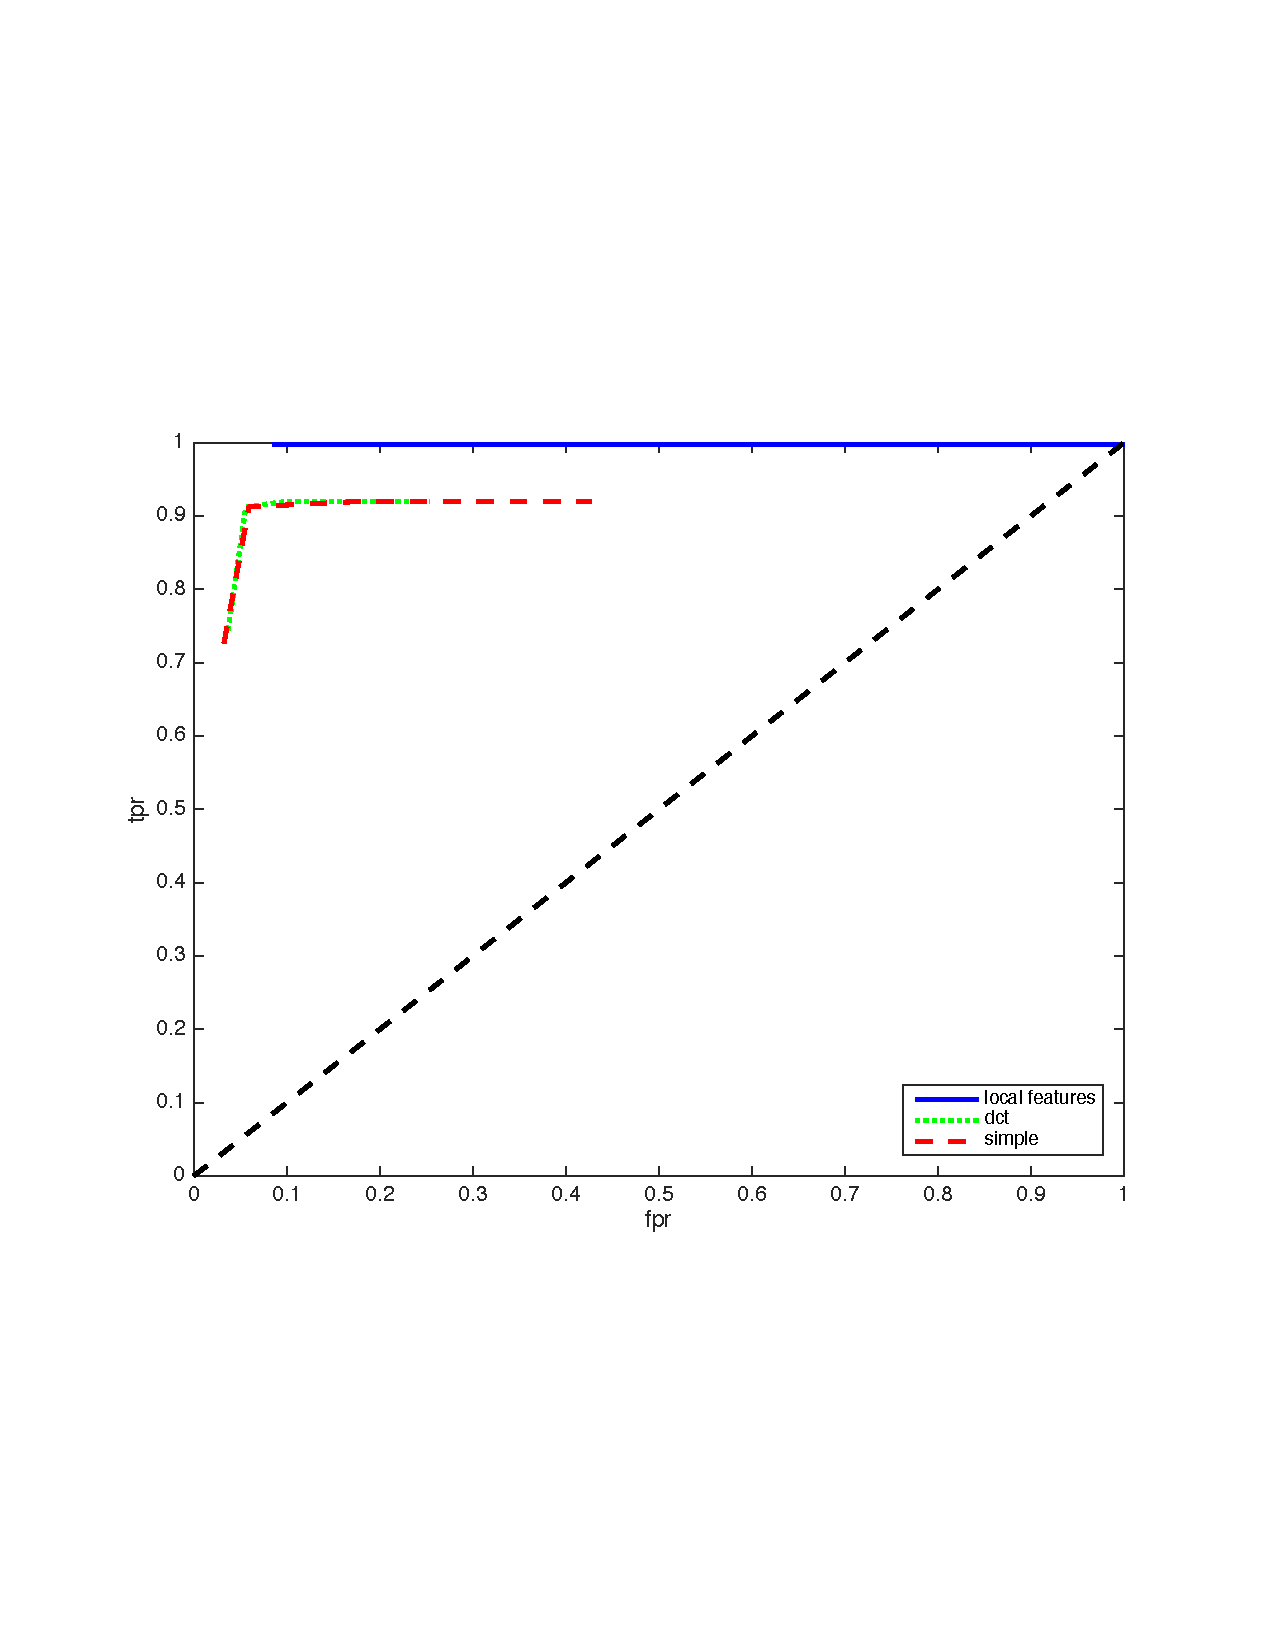
\includegraphics[width=\textwidth]{figures/thinglink_NormalizehistogramROC.pdf}
    \caption{ThingLink ROC}
    \label{Normalizepr}
  \end{subfigure}
  %
  \begin{subfigure}[b]{0.49\textwidth}
    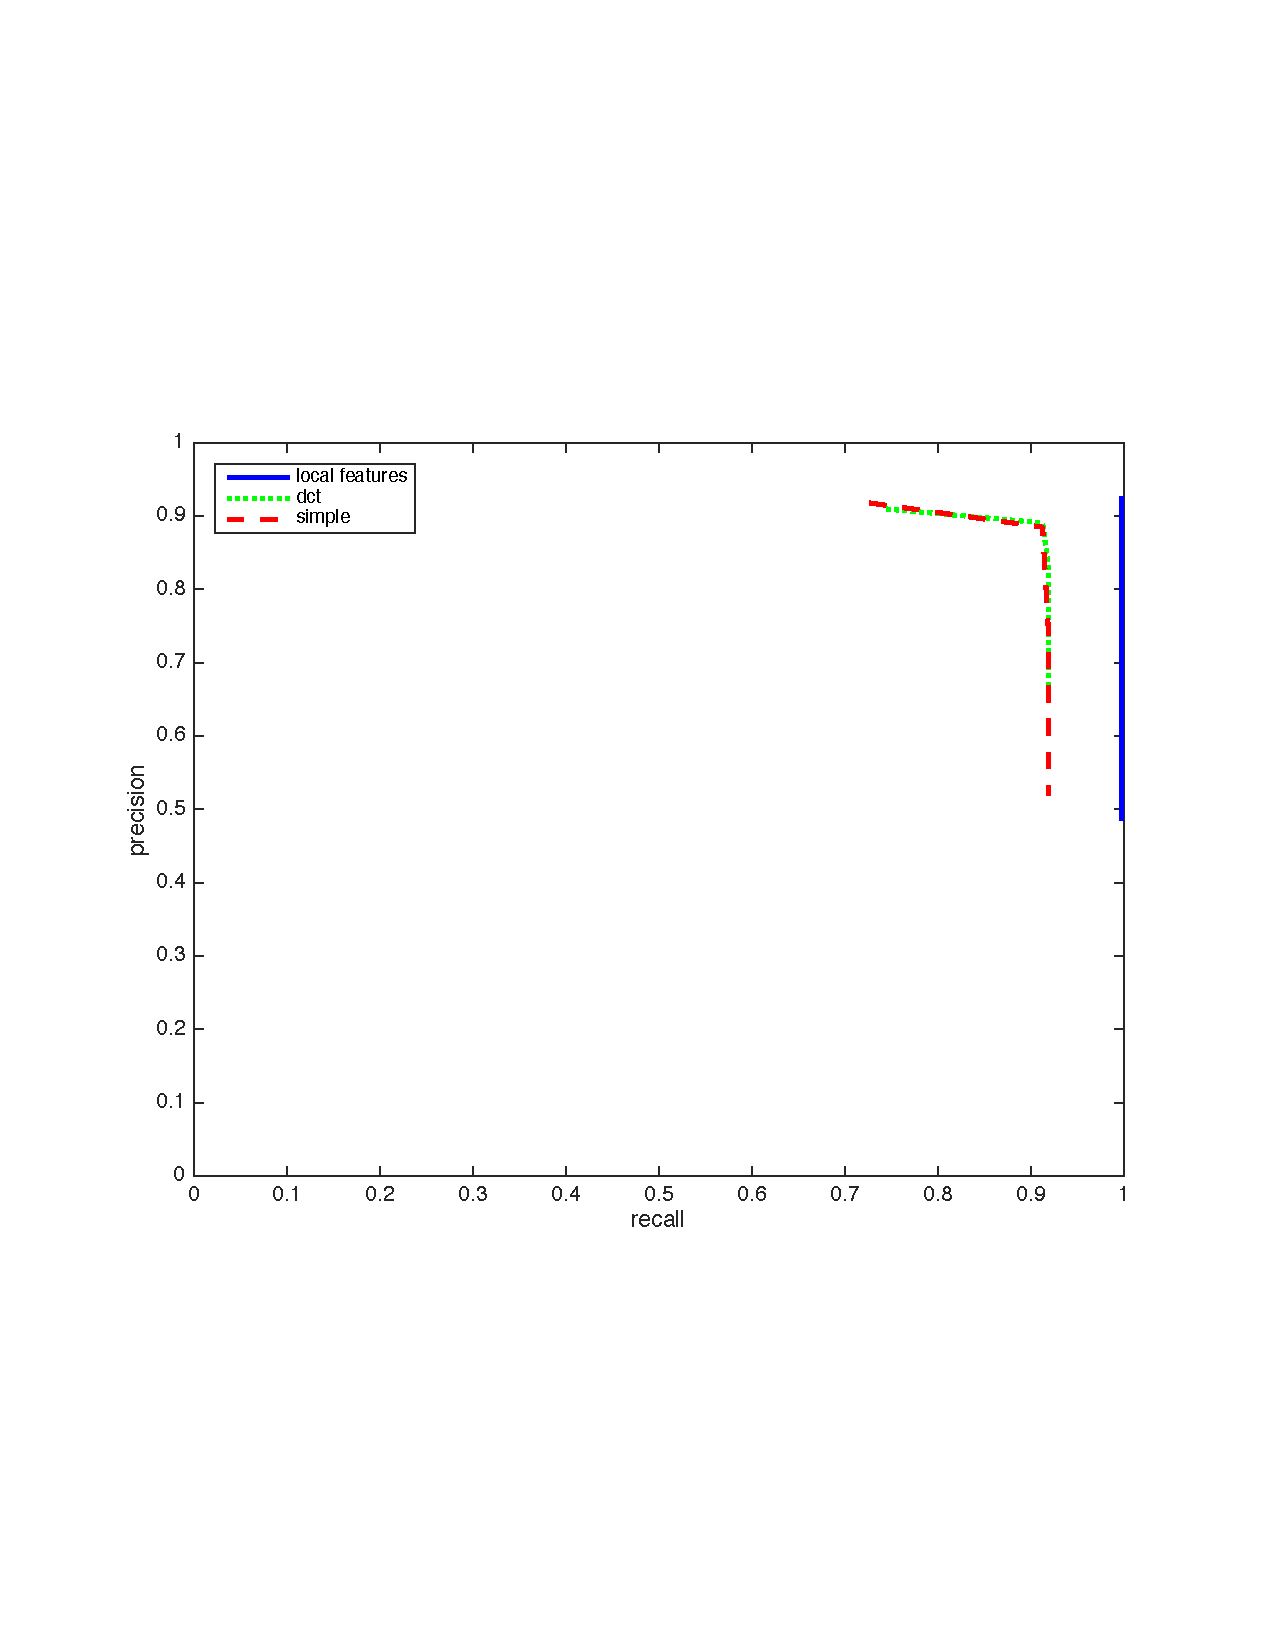
\includegraphics[width=\textwidth]{figures/thinglink_NormalizehistogramPR.pdf}
    \caption{ThingLink PR}
    \label{Normalizeprthinglink}
  \end{subfigure}
  \caption{\emph{Normalize histogram near-duplicate query results.} See figure \ref{53label} for a detailed caption. \label{histogramlabel}}
  \end{center}
\end{figure}

\begin{figure}[htb]
  \begin{center}
  \begin{subfigure}[b]{0.49\textwidth}
    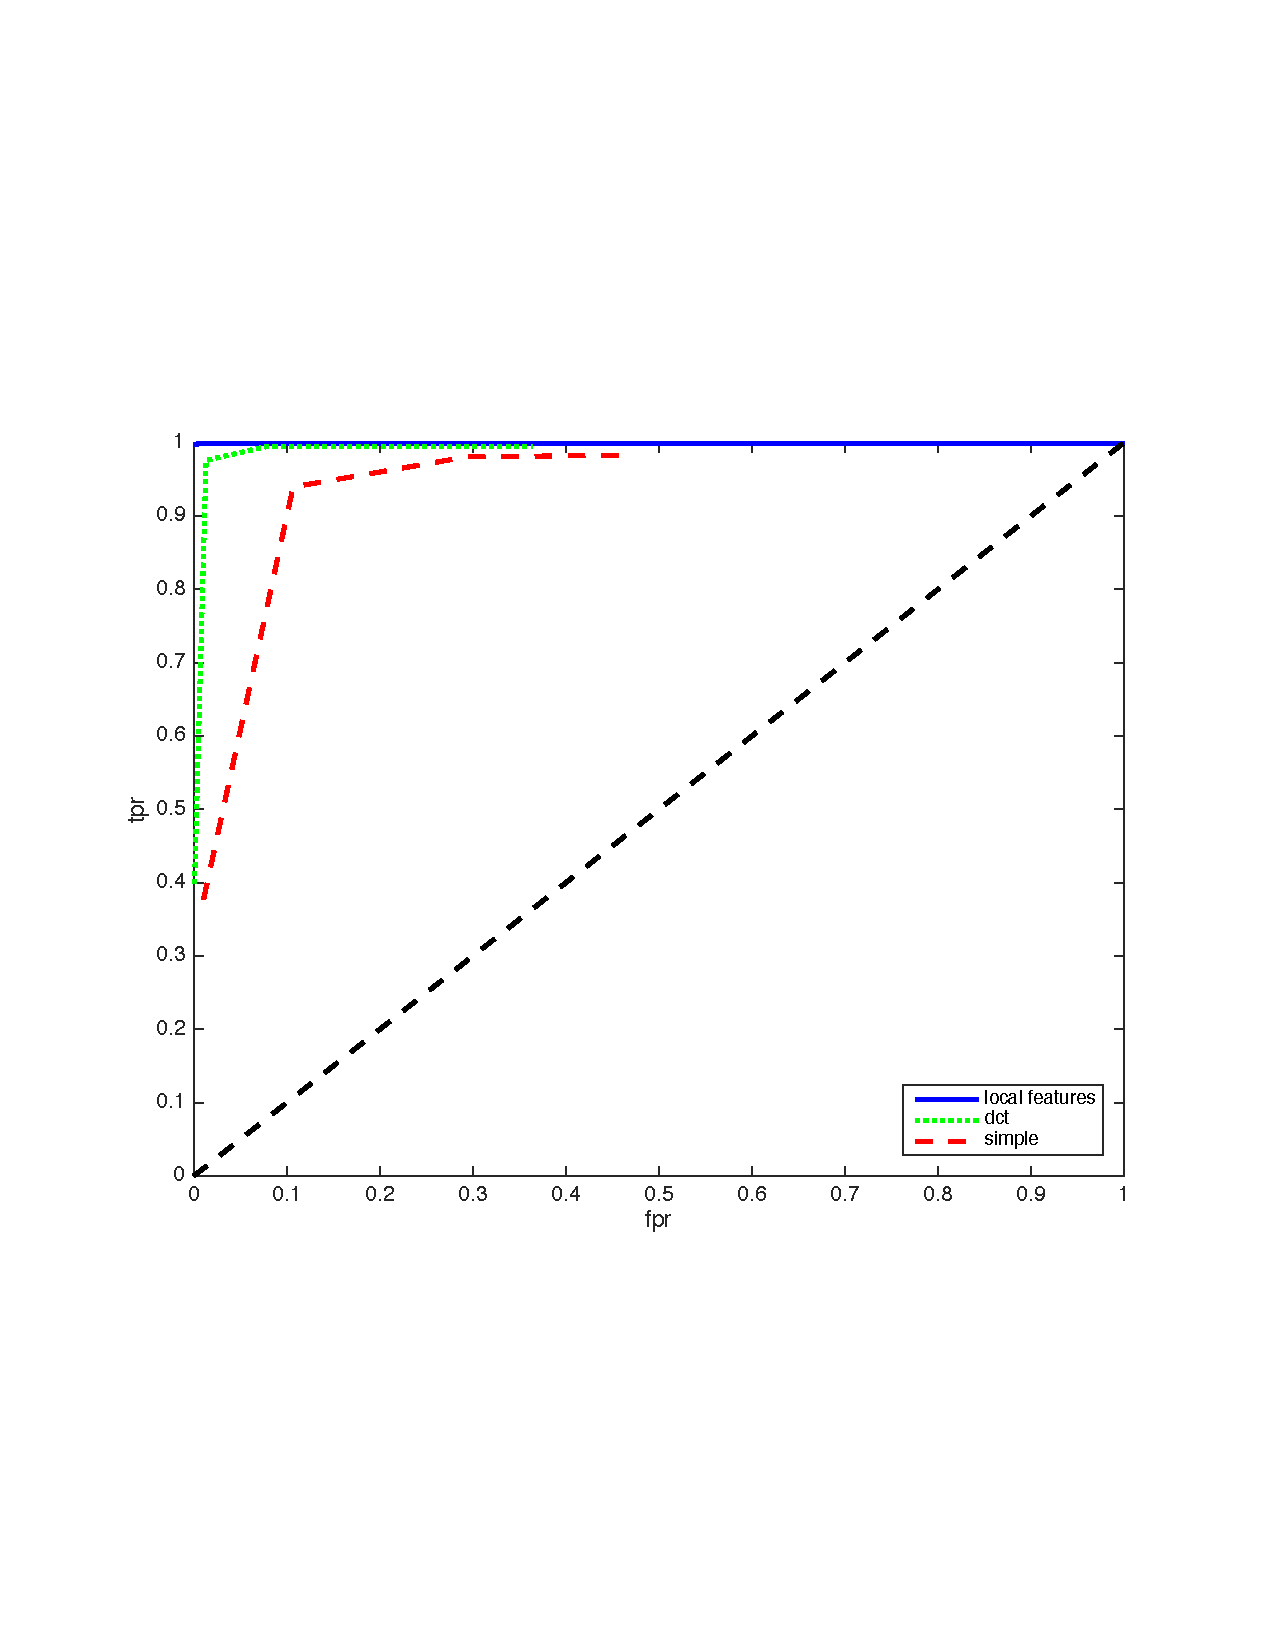
\includegraphics[width=\textwidth]{figures/SaturatecolorsROC.pdf}
    \caption{Paintings ROC}
    \label{Saturateroc}
  \end{subfigure}
  %
  \begin{subfigure}[b]{0.49\textwidth}
    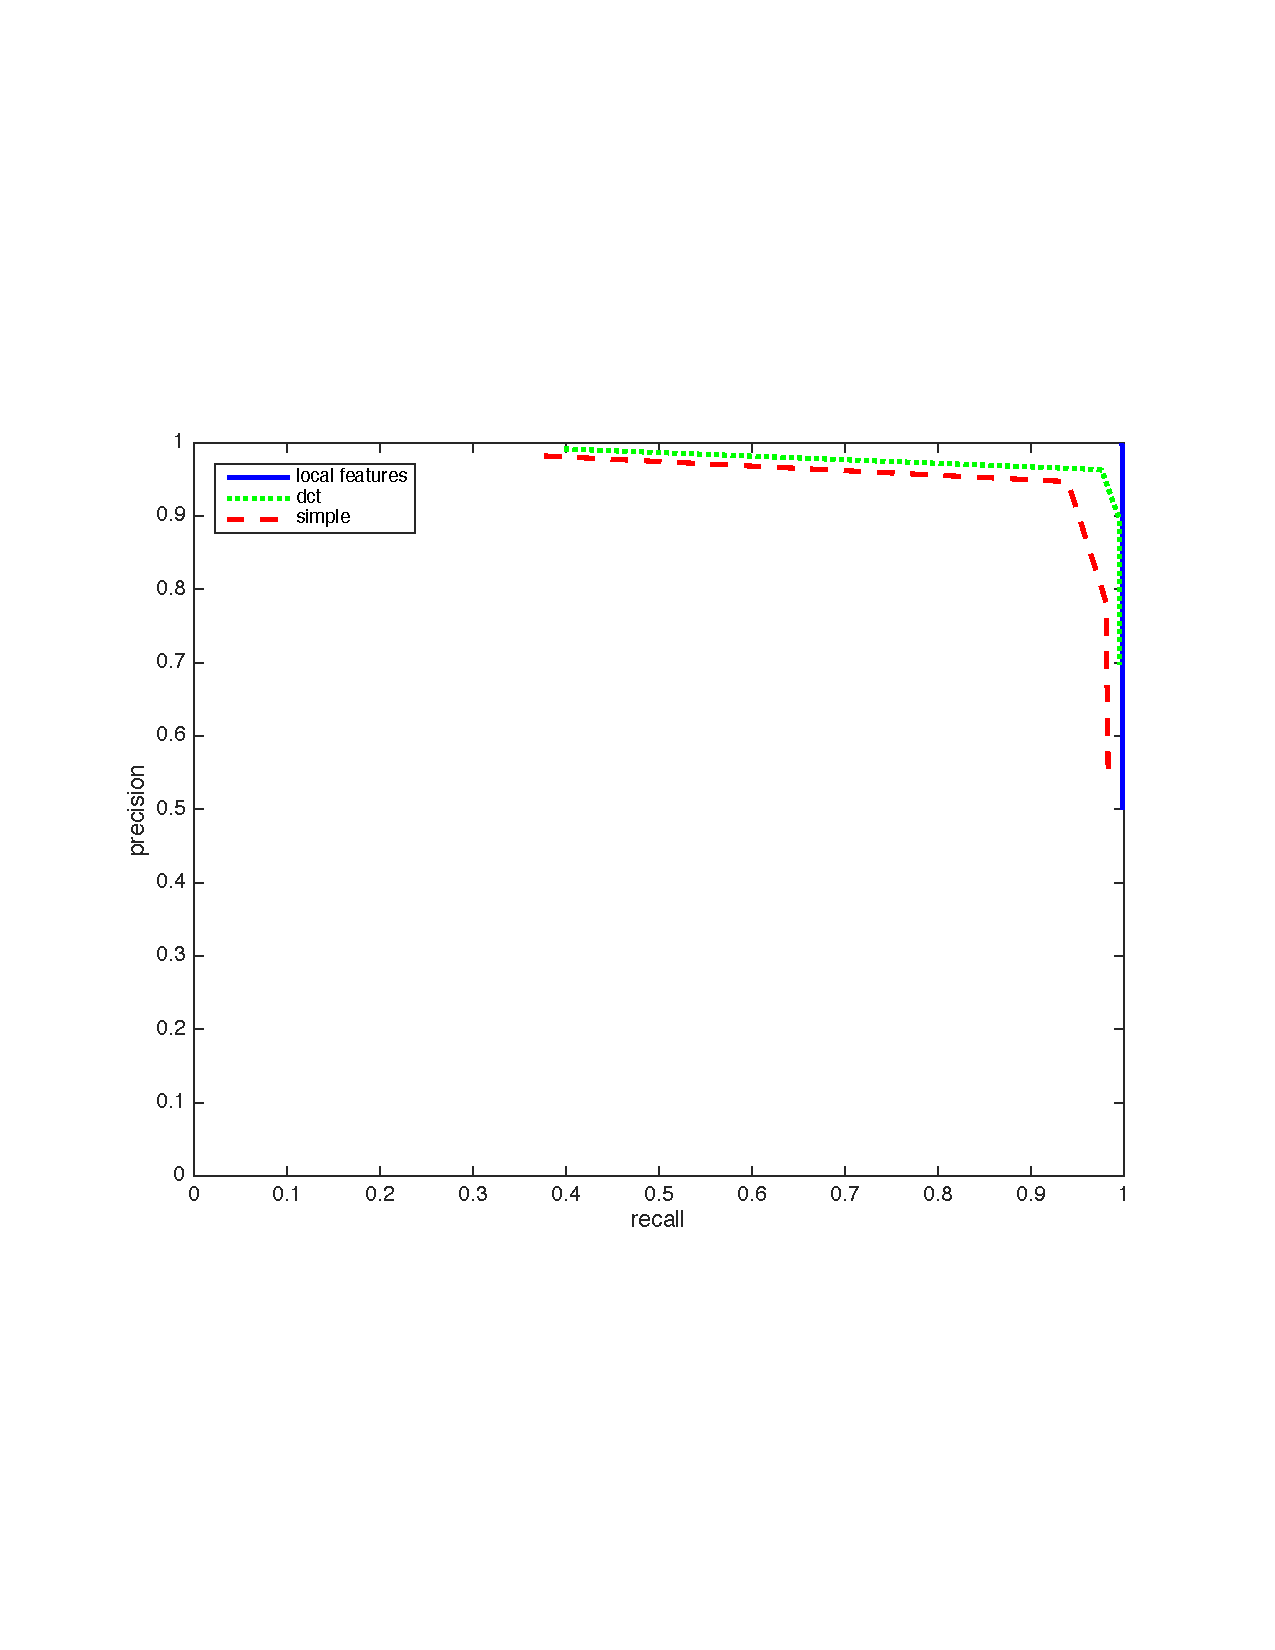
\includegraphics[width=\textwidth]{figures/SaturatecolorsPR.pdf}
    \caption{Paintings PR}
    \label{Saturaterocthinglink}
  \end{subfigure}
  \begin{subfigure}[b]{0.49\textwidth}
    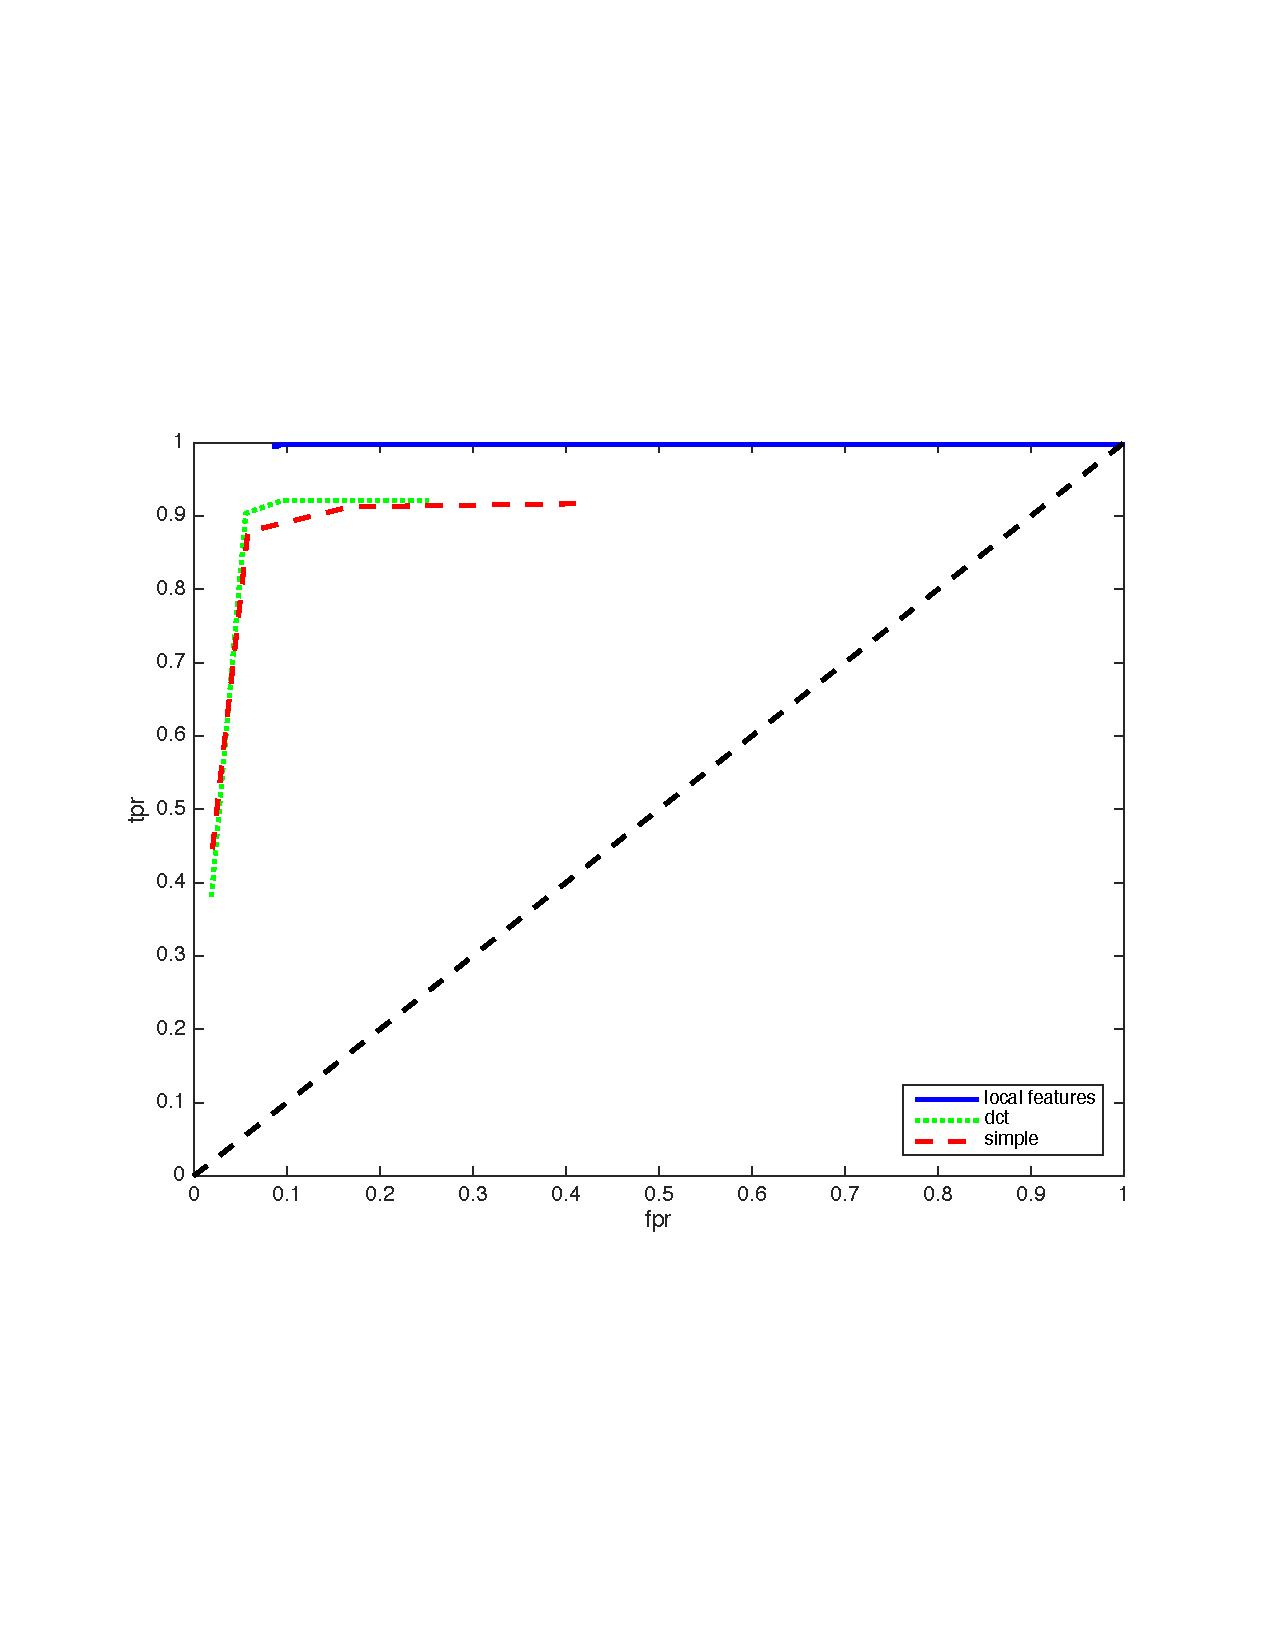
\includegraphics[width=\textwidth]{figures/thinglink_SaturatecolorsROC.pdf}
    \caption{ThingLink ROC}
    \label{Saturatepr}
  \end{subfigure}
  %
  \begin{subfigure}[b]{0.49\textwidth}
    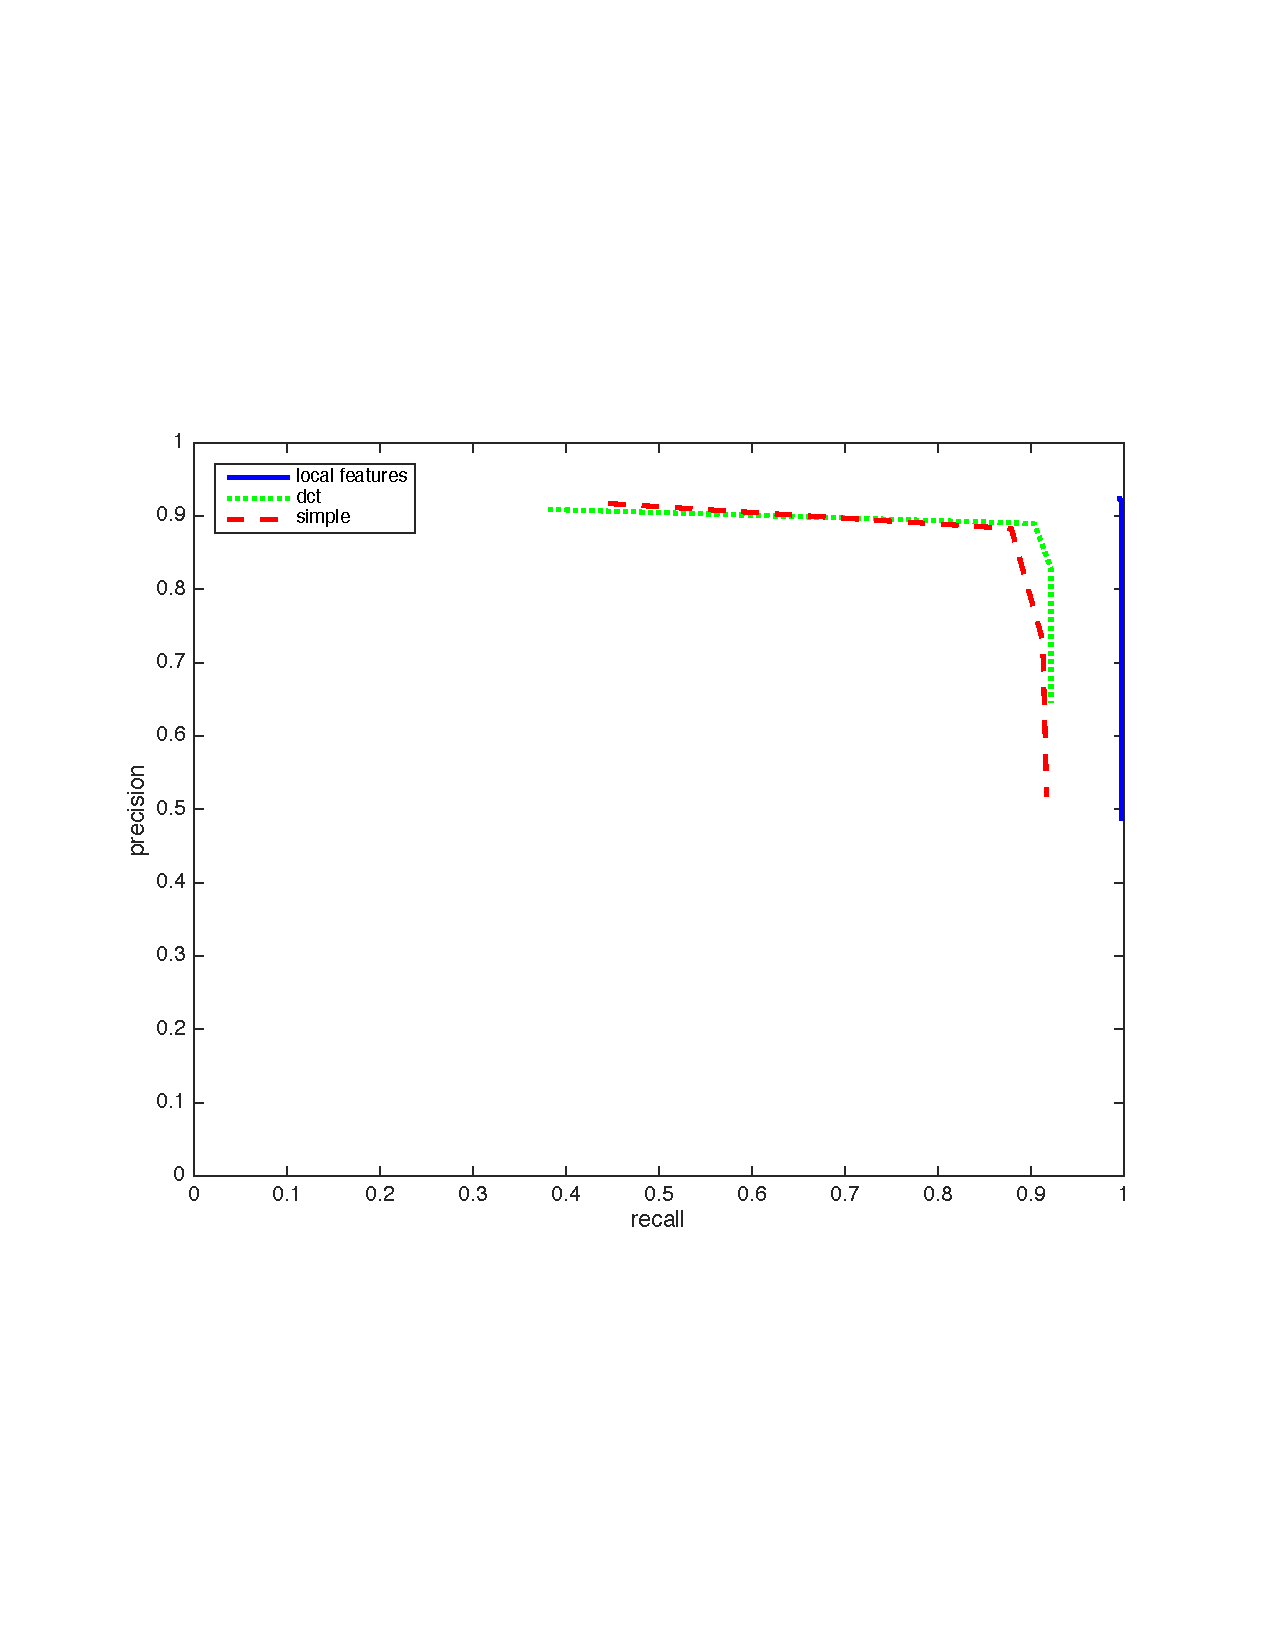
\includegraphics[width=\textwidth]{figures/thinglink_SaturatecolorsPR.pdf}
    \caption{ThingLink PR}
    \label{Saturateprthinglink}
  \end{subfigure}
  \caption{\emph{Saturate colors near-duplicate query results.} See figure \ref{53label} for a detailed caption.\label{saturatelabel}}
  \end{center}
\end{figure}


%% \begin{figure}[htb]
%% \begin{center}
%% 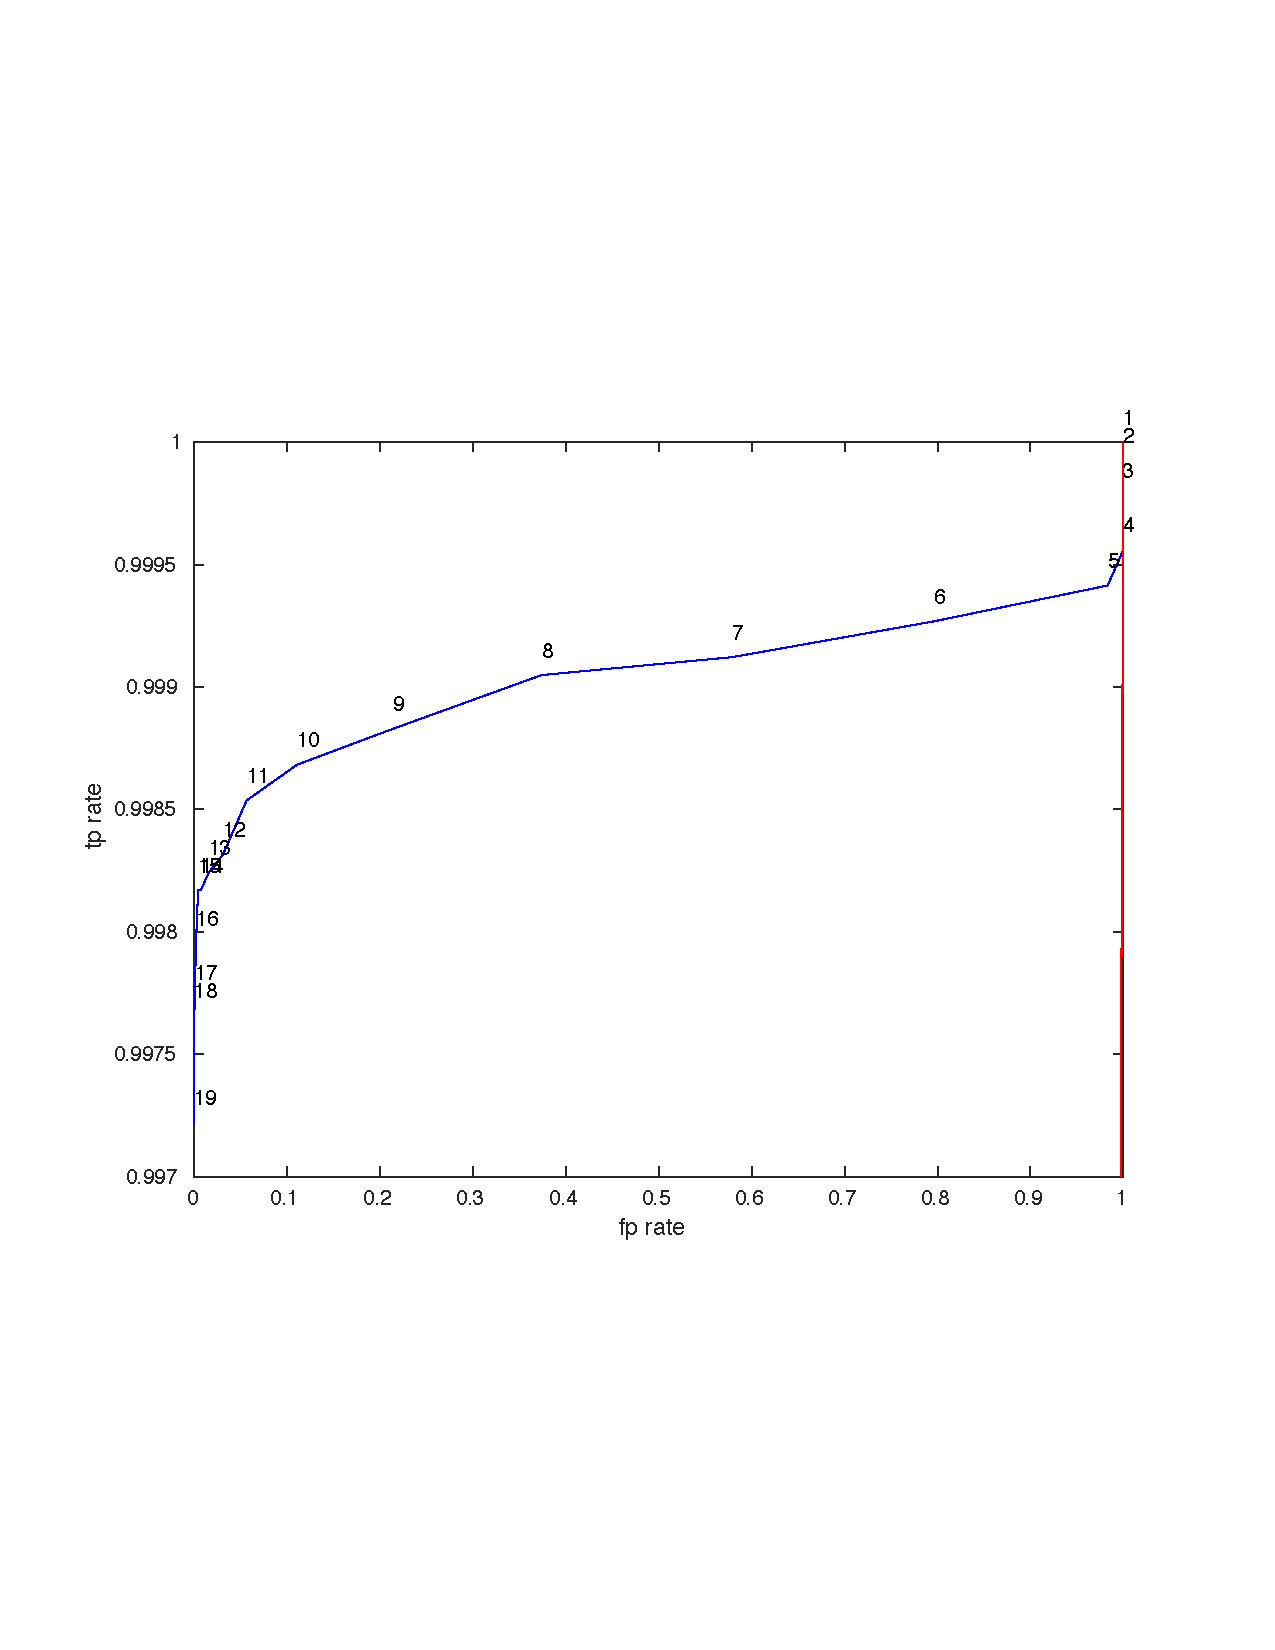
\includegraphics[height=8cm]{figures/SIFTROCperCutoff}
%% \end{center}
%% \caption{ Local Features NDID ROC Space for $0 < \mathcal{C}_{s} \leq 19$ built from query responses of duplicate sets in table \ref{modifiedimages}.}
%% \label{figcutoffrocspace}
%% \end{figure}

%% \begin{figure}[htb]
%% \begin{center}
%% 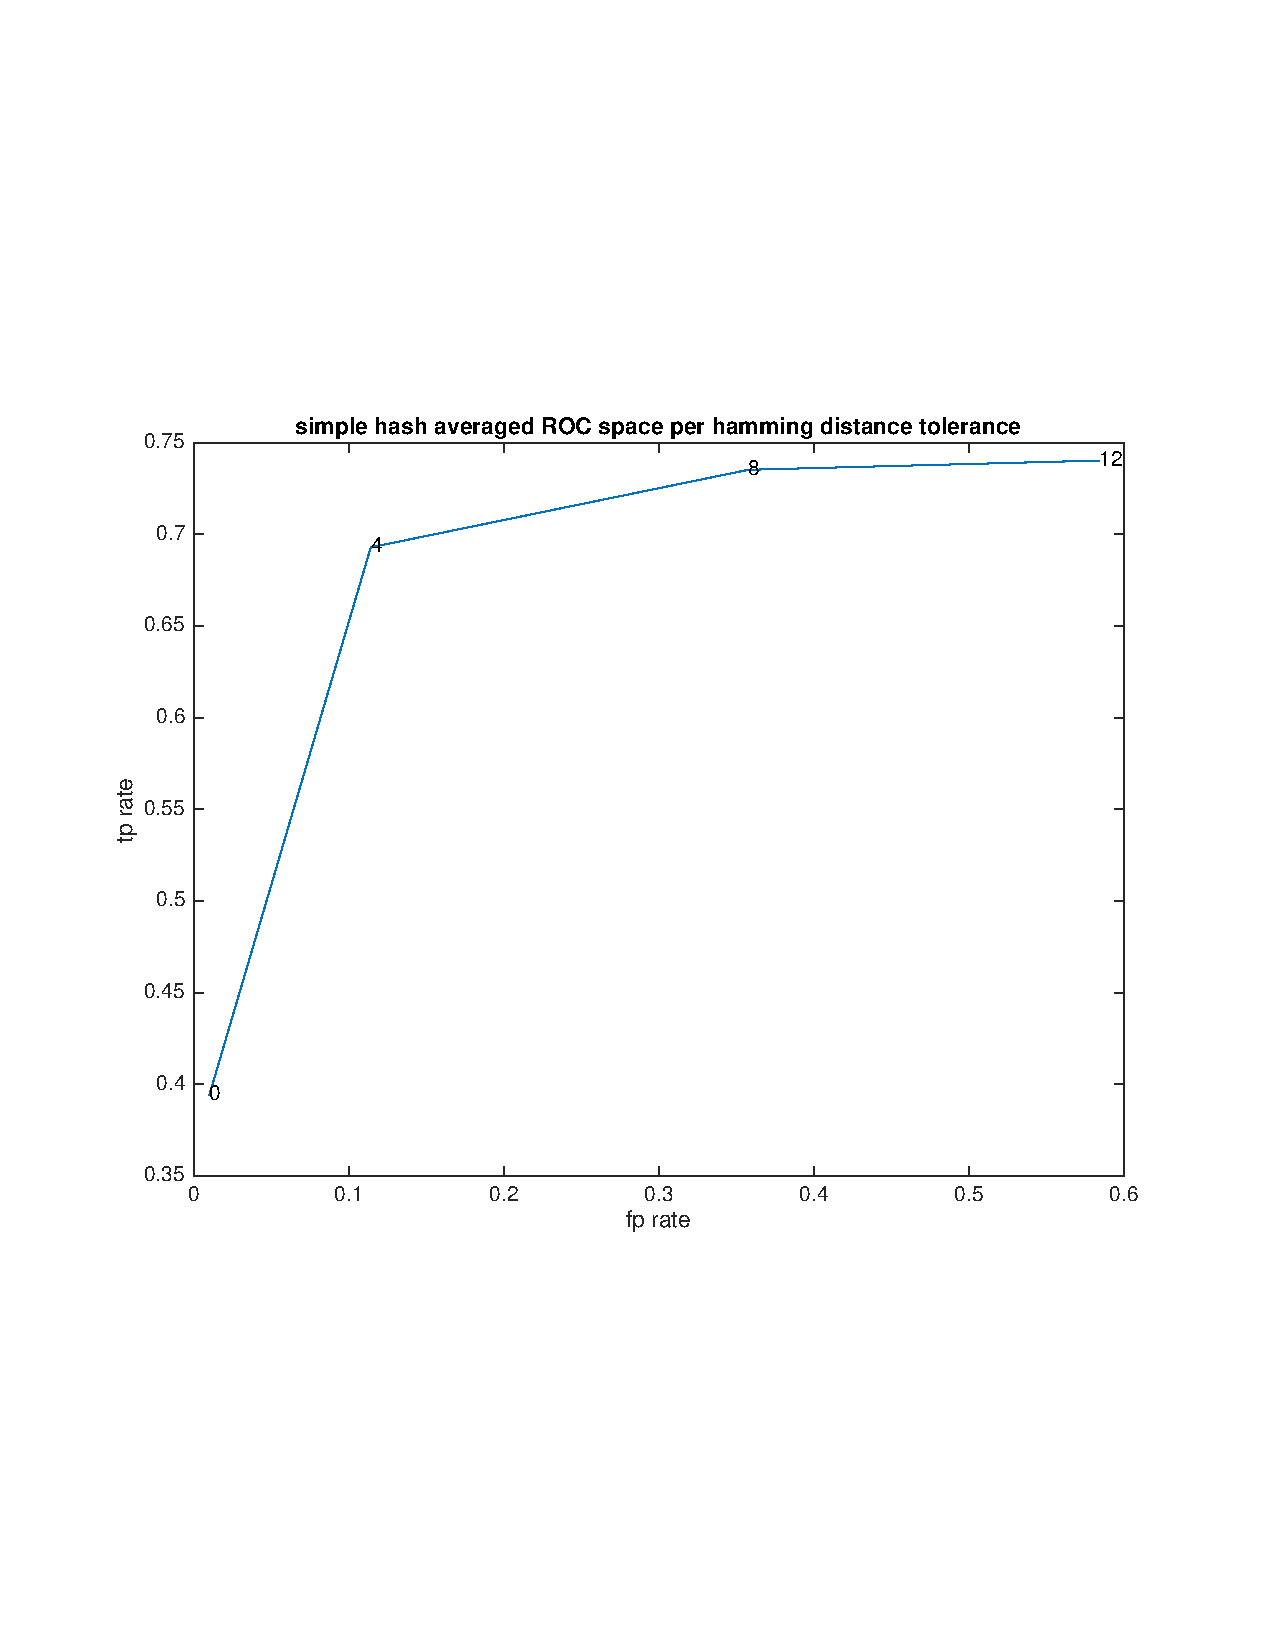
\includegraphics[height=8cm]{figures/simpleTotalROC}
%% \end{center}
%% \caption{Simple Hash NDID ROC space. Hamming Distance denoted at each ROC point. The ROC space points are based on averaging query results of all duplicate sets in table \ref{modifiedimages}. }
%% \label{simpletotalroc}
%% \end{figure}

%% \begin{figure}[htb]
%% \begin{center}
%% 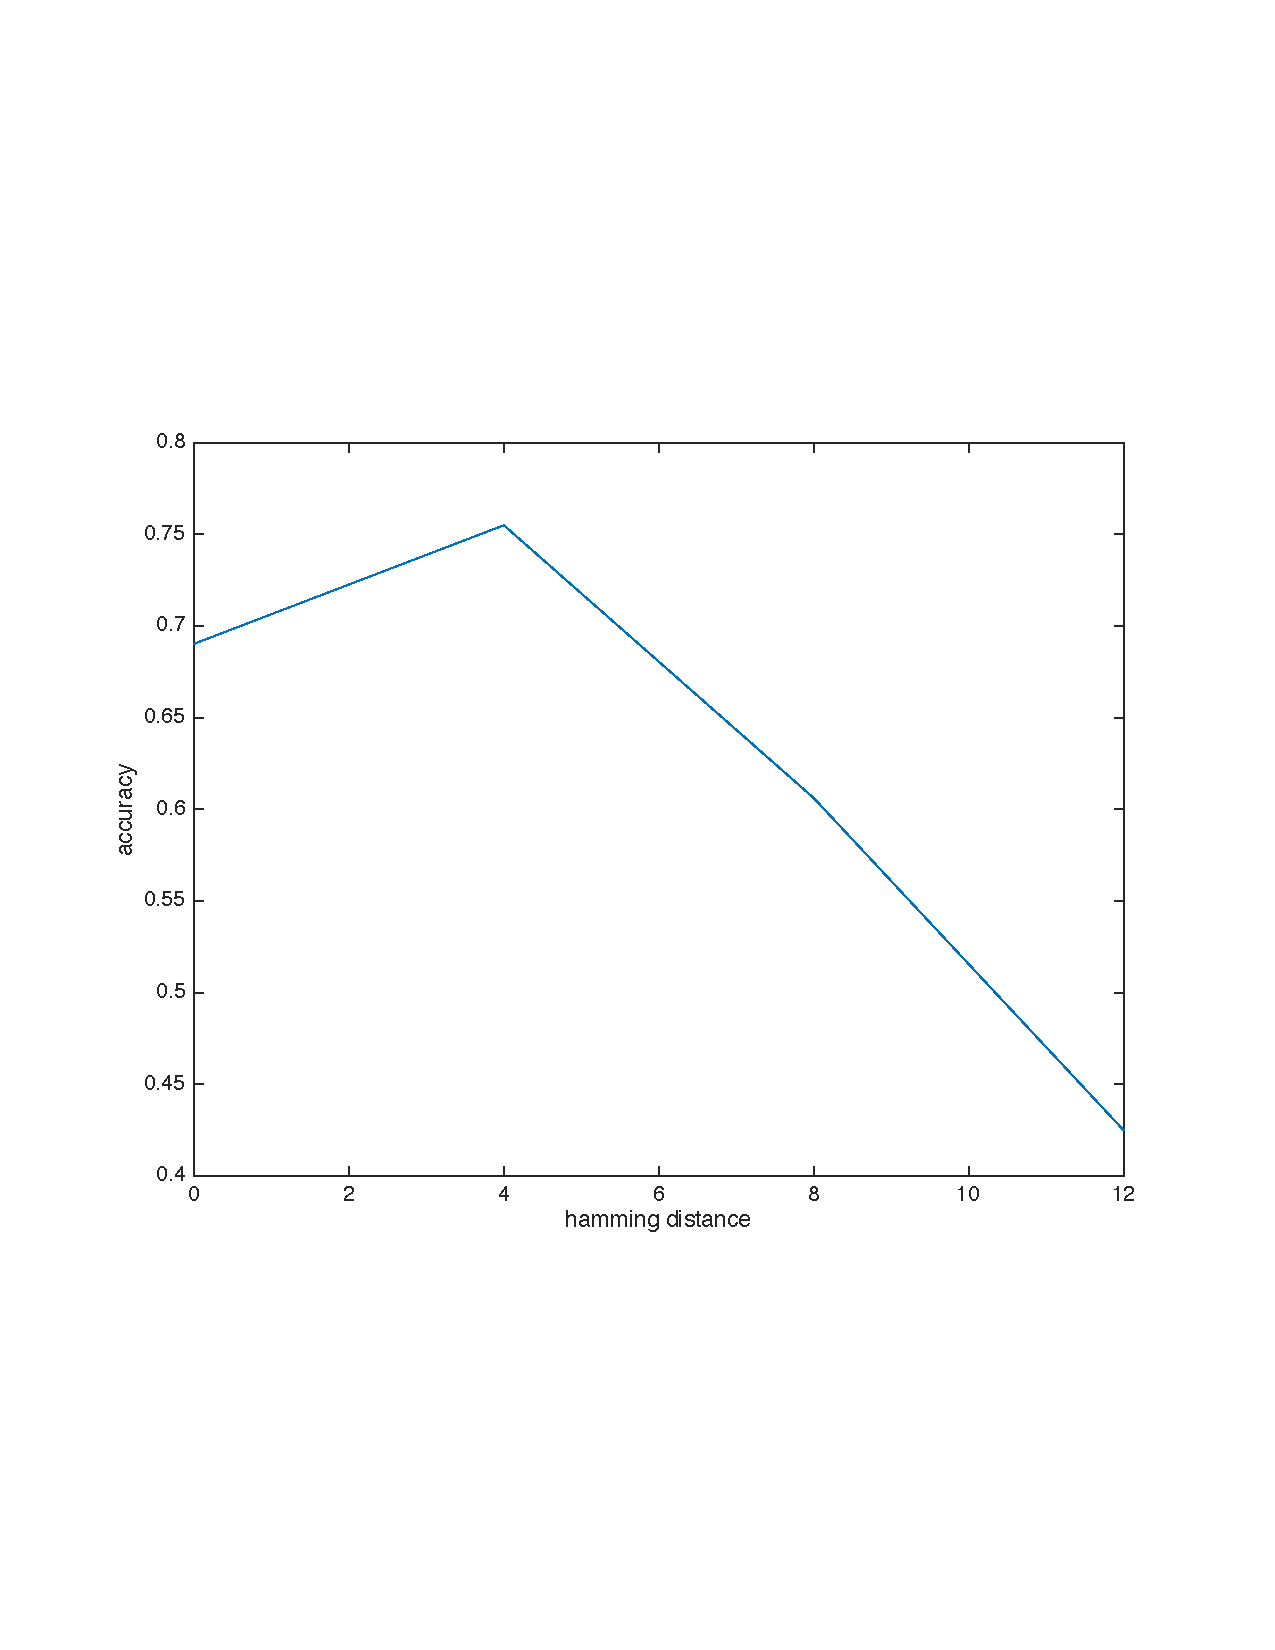
\includegraphics[height=8cm]{figures/simpleTotalAccuracy}
%% \end{center}
%% \caption{Simple Hash NDID accuracy (eq. \ref{accuracy}) per Hamming Distance averaged over all near-duplicate sets (table \ref{modifiedimages})}
%% \label{simpletotalaccuracy}
%% \end{figure}

%% \begin{figure}[htb]
%% \begin{center}
%% 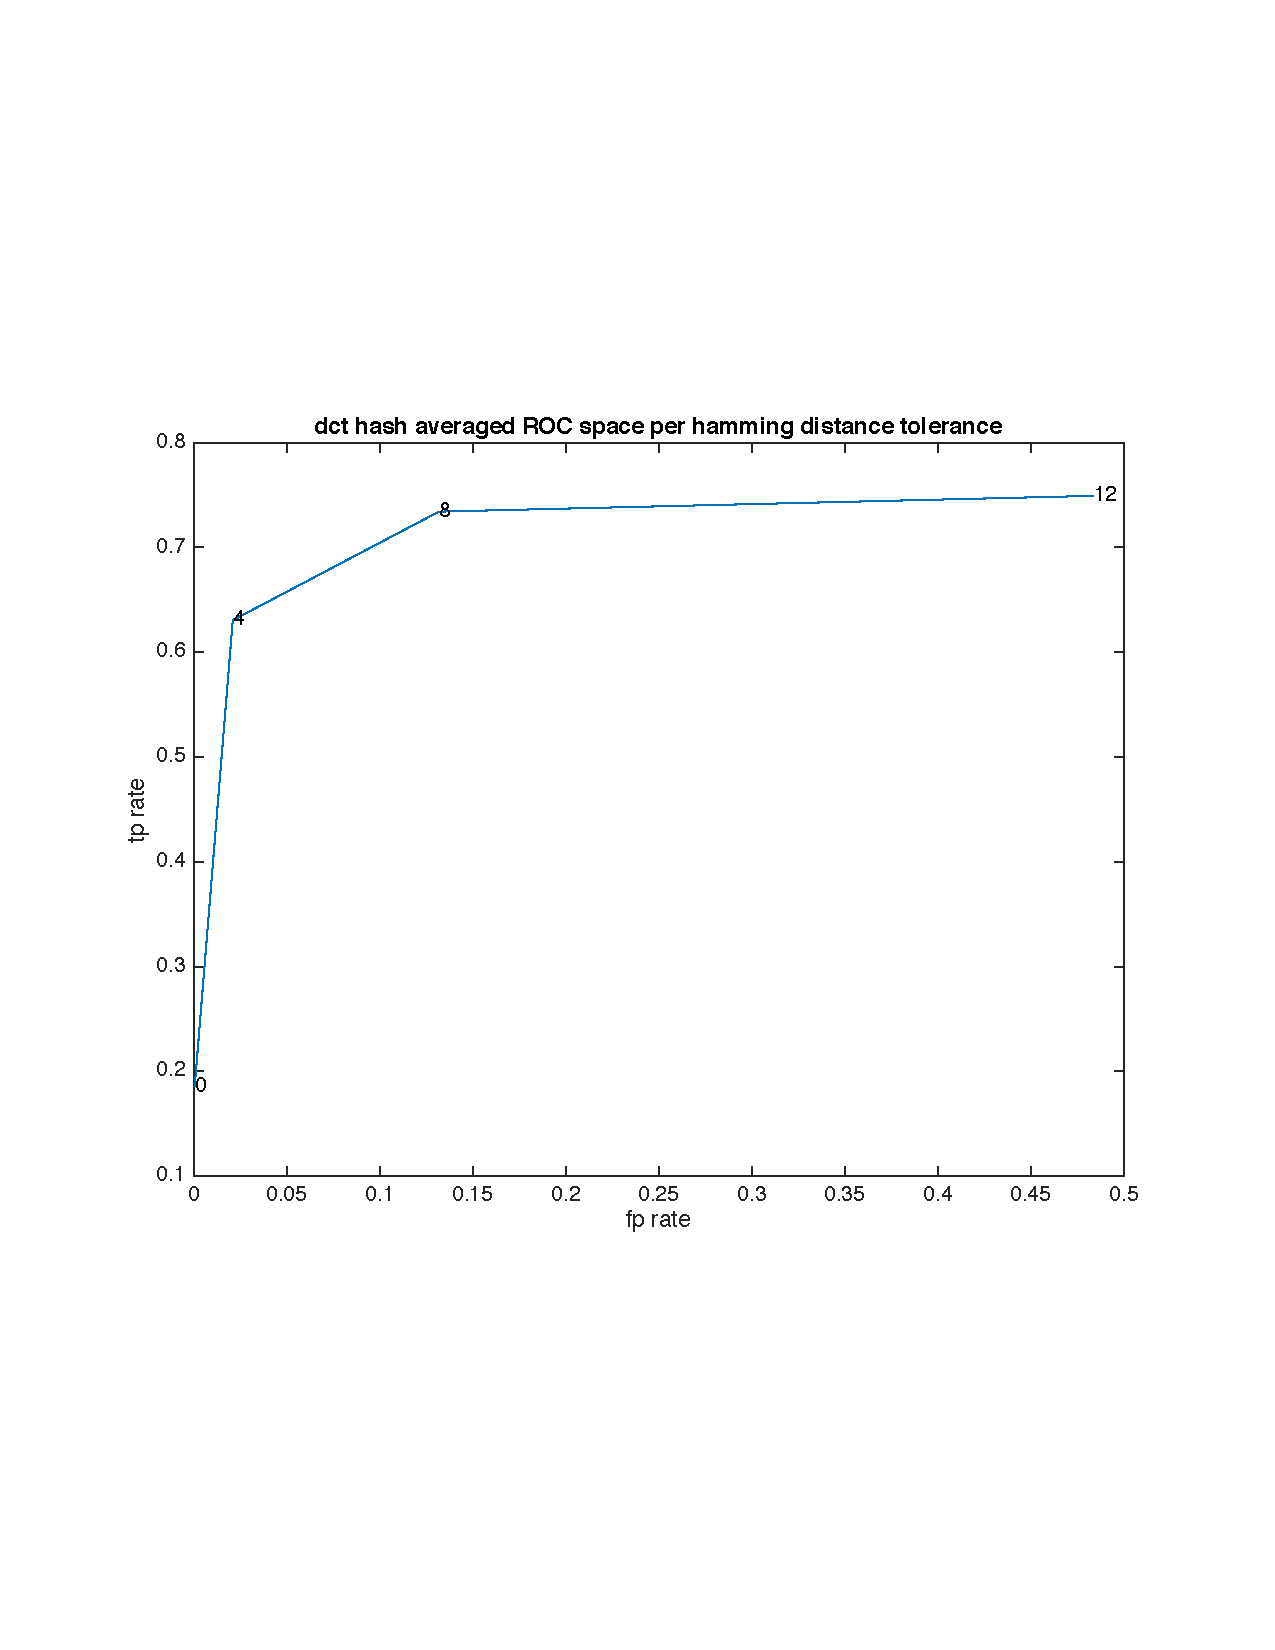
\includegraphics[height=8cm]{figures/dctTotalROC}
%% \end{center}
%% \caption{DCT Hash NDID average ROC space. Hamming Distance denoted at each ROC point. The ROC space points are based on averaging results of all duplicate sets in table \ref{modifiedimages}.}
%% \label{dcttotalroc}
%% \end{figure}

%% \begin{figure}[htb]
%% \begin{center}
%% 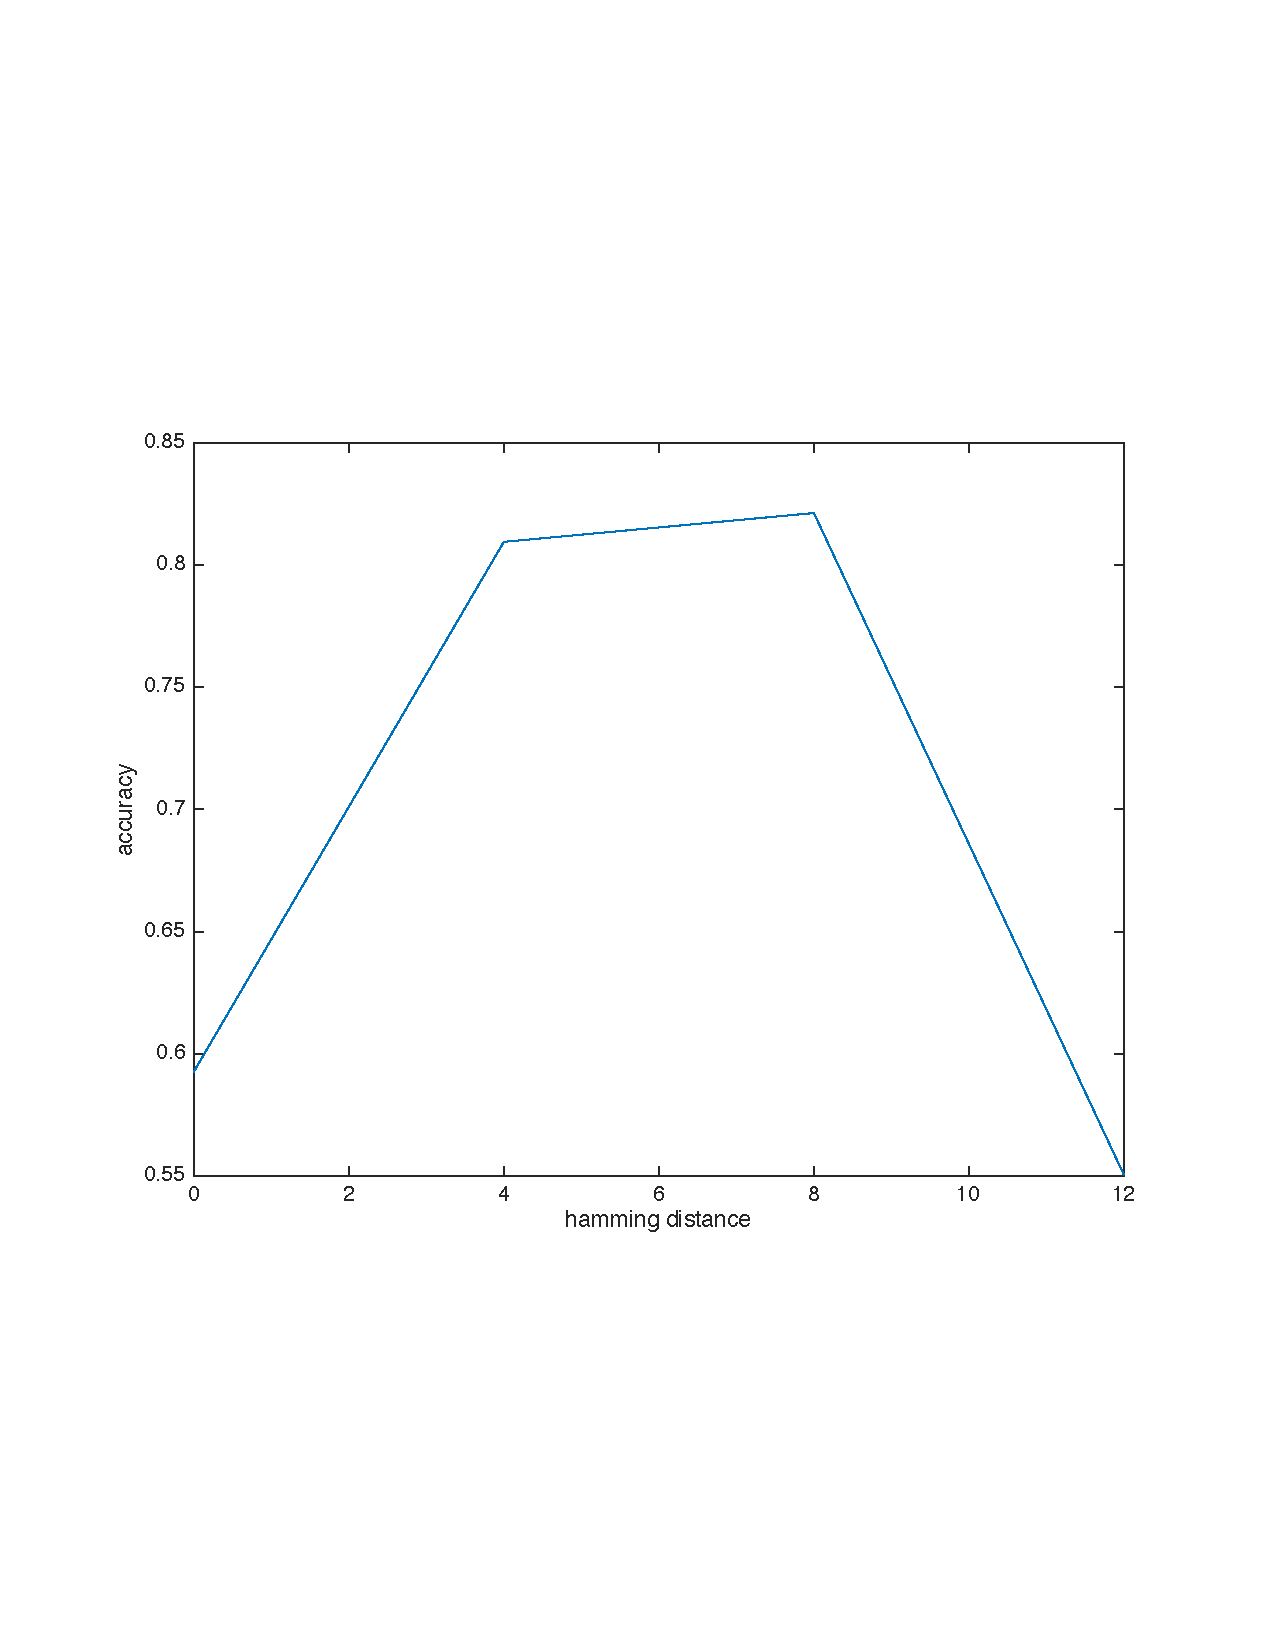
\includegraphics[height=8cm]{figures/dctTotalAccuracy}
%% \end{center}
%% \caption{DCT Hash NDID accuracy (eq. \ref{accuracy}) per Hamming Distance averaged over all near-duplicate sets (table \ref{modifiedimages})}
%% \label{dcttotalaccuracy}
%% \end{figure}

%% \begin{figure}[htb]
%% \begin{center}
%% \includegraphics[height=8cm]{figures/tpBar}
%% \end{center}
%% \caption{ TPR for near-duplicate modifications in table \ref{modifiedimages} for the Paintings dataset.}
%% \label{tptotal}
%% \end{figure}

%% \begin{figure}[htb]
%% \begin{center}
%% \includegraphics[height=8cm]{figures/fpBar}
%% \end{center}
%% \caption{ FPR for near-duplicate modifications in table \ref{modifiedimages} for the Paintings dataset.}
%% \label{fptotal}
%% \end{figure}

%% \begin{figure}[htb]
%% \begin{center}
%% \includegraphics[height=8cm]{figures/tnBar}
%% \end{center}
%% \caption{ TN for near-duplicate modifications for the Paintings dataset.}
%% \label{tntotal}
%% \end{figure}

%% \begin{figure}[htb]
%% \begin{center}
%% \includegraphics[height=8cm]{figures/thinglink_SIFTROCperCutoff}
%% \end{center}
%% \caption{ Local Features NDID ROC Space for $0 < \mathcal{C}_{s} \leq 16$ built from TN ThingLink dataset and duplicate sets in table \ref{modifiedimages}.}
%% \label{thinglinkfigcutoffrocspace}
%% \end{figure}

%% \begin{figure}[htb]
%% \begin{center}
%% \includegraphics[height=8cm]{figures/thinglink_simpleTotalROC}
%% \end{center}
%% \caption{Simple Hash NDID ROC space. Hamming Distance denoted at each ROC point. The ROC space points are based on averaging results of all duplicate sets in table \ref{modifiedimages} for the ThingLink dataset. }
%% \label{thinglinksimpletotalroc}
%% \end{figure}

%% \begin{figure}[htb]
%% \begin{center}
%% \includegraphics[height=8cm]{figures/thinglink_simpleTotalAccuracy}
%% \end{center}
%% \caption{Simple Hash NDID accuracy (eq. \ref{accuracy}) per Hamming Distance over all near-duplicate sets (table \ref{modifiedimages}) for the ThingLink dataset.}
%% \label{thinglinksimpletotalaccuracy}
%% \end{figure}

%% \begin{figure}[htb]
%% \begin{center}
%% \includegraphics[height=8cm]{figures/thinglink_dctTotalAccuracy}
%% \end{center}
%% \caption{DCT Hash NDID accuracy (eq. \ref{accuracy}) per Hamming Distance averaged over all near-duplicate sets (table \ref{modifiedimages}) for the ThingLink dataset.}
%% \label{thinglinkdcttotalaccuracy}
%% \end{figure}

%% \begin{figure}[htb]
%% \begin{center}
%% \includegraphics[height=8cm]{figures/thinglink_dctTotalROC}
%% \end{center}
%% \caption{DCT Hash NDID average ROC space. Hamming Distance denoted at each ROC point. The ROC space points are based on averaging results of all duplicate sets in table \ref{modifiedimages} for the ThingLink dataset.}
%% \label{thinglinkdcttotalroc}
%% \end{figure}

%% \begin{figure}[htb]
%% \begin{center}
%% \includegraphics[height=8cm]{figures/thinglink_tpBar}
%% \end{center}
%% \caption{ TPR for near-duplicate modifications in table \ref{modifiedimages} for the ThingLink dataset.}
%% \label{thinglinktptotal}
%% \end{figure}

%% \begin{figure}[htb]
%% \begin{center}
%% \includegraphics[height=8cm]{figures/thinglink_fpBar}
%% \end{center}
%% \caption{ FPR for near-duplicate modifications in table \ref{modifiedimages} for the ThingLink dataset.}
%% \label{thinglinkfptotal}
%% \end{figure}

%% \begin{figure}[htb]
%% \begin{center}
%% \includegraphics[height=8cm]{figures/thinglink_tnBar}
%% \end{center}
%% \caption{ TNR for near-duplicate modifications for the ThingLink dataset.}
%% \label{thinglinktntotal}
%% \end{figure}

\begin{table*} \footnotesize
  \caption{Computational cost. $t_f^{avg}$ (ms) is the average time to calculate a single image descriptor or hash value. $s_f$ (bits) is the size of the descriptor or hash in bits. $t_q^{avg}$ (ms) is the average query time from the database and $db$ (MB) is the database size in memory. For Local Features, 99\% of the query time $t_q^{avg}$ goes in geometric verification.}
\label{computationalcost}
\begin{center}
  \setlength\tabcolsep{3pt} % default value: 6pt
  \begin{tabular}{@{}lcrcrrcrcr@{}}
    \toprule
    & \multicolumn{4}{c}{Paintings} &\phantom{abc} &\multicolumn{4}{c}{ThingLink}\\
\cmidrule{2-6} \cmidrule{7-10}
  & $t_f^{avg} $&  $s_f$ & $t_q^{avg}$& $db$ &\phantom{abc} & $t_f^{avg} $&  $s_f$& $t_q^{avg}$& $db$\\ \midrule
    Local Features & 257 & $64 \times 10^5$ & 800 & 300&\phantom{abc} & 81 & $64 \times 10^5$& 122 &95\\
    Simple & 126 & 64 & 329 & 0.071 &\phantom{abc} & 14 & 64 & 187 & 0.017\\
    DCT   & 133 & 64 & 338 & 0.071 & \phantom{abc} & 118 & 64 & 77 & 0.017\\
 \bottomrule
\end{tabular}
\end{center}\end{table*}

%% \begin{table}[htb]\footnotesize
%% \caption{ Simple Hash NDID results for duplicate sets (table \ref{modifiedimages}) for Paintings data from \cite{Vedaldi2012}. }
%% \label{simpleresults}
%% \begin{center}
%%   \setlength\tabcolsep{3pt} % default value: 6pt
%%   \begin{tabular}{@{}lrrrrrrrrrrrrrrr@{}}
%%     \toprule
%%     & \multicolumn{3}{c}{$\Delta(q,d) = 0$} &\phantom{abc} &\multicolumn{3}{c}{$\Delta(q,d) = 4$} &\phantom{abc} & \multicolumn{3}{c}{$\Delta(q,d)=8$} &\phantom{abc} & \multicolumn{3}{c}{$\Delta(q,d)=12$}\\
%% \cmidrule{2-4} \cmidrule{6-8} \cmidrule{10-12} \cmidrule{14-16}
%%     Modification & FP & TP & FN &\phantom{abc} & FP & TP & FN &\phantom{abc} & FP & TP & FN &\phantom{abc} & FP & TP & FN\\ \midrule
%%     53\% Scale   & 9 & 1612 & 87 &\phantom{abc} & 11 & 1696 & 1 &\phantom{abc} & 11 & 1697 & 0 &\phantom{abc} & 11 & 1697 & 0\\
%%     83\% Scale   & 9 & 1633 & 66 &\phantom{abc} & 10 & 1698 & 0 &\phantom{abc} & 10 & 1698 & 0 &\phantom{abc} & 10 & 1698 & 0\\
%%     Crop 10px    & 9 & 370 & 1329 &\phantom{abc} & 22 & 1553 & 133 &\phantom{abc} & 27 & 1667 & 14 &\phantom{abc} & 33 & 1675 & 0\\
%%     10\% Border  & 1 & 0 & 1707 & \phantom{abc} & 214 & 10 & 1484 &\phantom{abc} & 1079 & 23 & 606 &\phantom{abc} & 1639 & 29 & 40\\
%%     Rotate 10\%  & 0 & 0 & 1708 &\phantom{abc} & 68 & 6 & 1634 &\phantom{abc} & 737 & 19 & 952 &\phantom{abc} & 1568 & 32 & 108\\
%%     Normalize    & 7 & 987 & 714 &\phantom{abc} & 15 & 1653 & 40 &\phantom{abc} & 20 & 1679 & 9 &\phantom{abc} & 26 & 1682 & 0\\
%%     Saturate     & 8 & 644 & 1056 &\phantom{abc} & 25 & 1605 & 78 &\phantom{abc} & 28 & 1675 & 5 &\phantom{abc} & 29 & 1679 & 0\\
%%     Predicted Negative     & 28 & 0 & 0 &\phantom{abc} & 340 & 0 & 0 &\phantom{abc} & 976 & 0 & 0 &\phantom{abc} & 1571& 0& 0\\

%%     \bottomrule
%% \end{tabular}
%% \end{center}
%% \end{table}

\begin{sidewaystable}[htb]\footnotesize
\caption{ Simple Hash NDID unbiased metrics, \emph{Markedness} $\mathcal{M}$ (eq. \ref{markedness}), \emph{Informedness} $\mathcal{I}$ (eq. \ref{markedness}) and Matthews correlation $\mathcal{R}_G$ (eq. \ref{matthewscorrelation}) for duplicate sets (table \ref{modifiedimages}) for Paintings dataset. }
\label{simpleunbiased}
\begin{center}
  \setlength\tabcolsep{3pt} % default value: 6pt
  \begin{tabular}{@{}lrrrrrrrrrrrrrrr@{}}
    \toprule
    & \multicolumn{3}{c}{$\Delta(q,d) = 0$} &\phantom{abc} &\multicolumn{3}{c}{$\Delta(q,d) = 4$} &\phantom{abc} & \multicolumn{3}{c}{$\Delta(q,d)=8$} &\phantom{abc} & \multicolumn{3}{c}{$\Delta(q,d)=12$}\\
\cmidrule{2-4} \cmidrule{6-8} \cmidrule{10-12} \cmidrule{14-16}
    Modification & $\mathcal{I}$ & $\mathcal{M}$ & $\mathcal{R}_G$ &\phantom{abc} & $\mathcal{I}$ & $\mathcal{M}$ & $\mathcal{R}_G$ &\phantom{abc} & $\mathcal{I}$ & $\mathcal{M}$ & $\mathcal{R}_G$ &\phantom{abc} & $\mathcal{I}$ & $\mathcal{M}$ & $\mathcal{R}_G$\\ \midrule
    53\% Scale   & 0.9272 & 0.9283& 0.9278  &\phantom{abc} & 0.7952 & 0.8278 & 0.8113 &\phantom{abc} & 0.4258 & 0.6323 & 0.5189 &\phantom{abc} & 0.0797 & 0.5175 & 0.2031\\
    83\% Scale   & 0.9396 & 0.9400 & 0.9398 &\phantom{abc} & 0.7963 & 0.8291 & 0.8125 &\phantom{abc} & 0.4261 & 0.6326 & 0.5192 &\phantom{abc} & 0.0797 & 0.5178 & 0.2032 \\
    Crop 10px    & 0.1962  & 0.4674  & 0.3029 &\phantom{abc} & 0.7119 & 0.7224 & 0.7171 &\phantom{abc} & 0.4136 & 0.6056 & 0.5005 &\phantom{abc} & 0.0704 & 0.4181 & 0.1716\\
    10\% Border  & -0.0170 & -0.5040 & 0.0925 & \phantom{abc} & -0.2815 & -0.5026 & 0.3762&\phantom{abc} & -0.7008 & -0.4418& 0.5565 &\phantom{abc} & -0.9134 & -0.8067 & 0.8584\\
    Rotate 10\%  & 0-0.0164 &  -0.5041&  0.0909 &\phantom{abc} & -0.2261 & -0.5298 & 0.3461 &\phantom{abc} & -0.6810& -0.5544 & 0.6144 &\phantom{abc} & -0.9257& -0.8641& 0.8944\\
    Normalize    & 0.5598 & 0.6675 & 0.6113 &\phantom{abc} &  0.7703 & 0.7948 & 0.7825 &\phantom{abc} & 0.4183 & 0.6180 & 0.5085 &\phantom{abc} & 0.0737 & 0.4513 & 0.1824\\
    Saturate     & 0.3578 & 0.5611 &  0.4481 &\phantom{abc} & 0.7430  & 0.7608 & 0.7519&\phantom{abc} & 0.4187 & 0.6184 & 0.5089 &\phantom{abc} & 0.0759& 0.4768 & 0.1902\\
    \bottomrule
    Average      & 0.4211 & 0.3652 & 0.4876 & \phantom{abc} & \cellcolor{blue!25}0.4727 & 0.4146 & 0.6568 & \phantom{abc} & 0.1030 & 0.3015 & 0.5324 &\phantom{abc} & -0.2085 & 0.1016 & 0.3862\\
\end{tabular}
\end{center}
\end{sidewaystable}



%% \begin{table}[htb]\footnotesize
%% \caption{ Simple Hash NDID results for duplicate sets (table \ref{modifiedimages}) for ThingLink dataset. }
%% \label{simplethinglinkresults}
%% \begin{center}
%%   \setlength\tabcolsep{3pt} % default value: 6pt
%%   \begin{tabular}{@{}lrrrrrrrrrrrrrrr@{}}
%%     \toprule
%%     & \multicolumn{3}{c}{$\Delta(q,d) = 0$} &\phantom{abc} &\multicolumn{3}{c}{$\Delta(q,d) = 4$} &\phantom{abc} & \multicolumn{3}{c}{$\Delta(q,d)=8$} &\phantom{abc} & \multicolumn{3}{c}{$\Delta(q,d)=12$}\\
%% \cmidrule{2-4} \cmidrule{6-8} \cmidrule{10-12} \cmidrule{14-16}
%%     Modification & FP & TP & FN &\phantom{abc} & FP & TP & FN &\phantom{abc} & FP & TP & FN &\phantom{abc} & FP & TP & FN\\ \midrule
%%     53\% Scale   & 34 & 357 & 55 &\phantom{abc} & 11 & 409 & 26 &\phantom{abc} & 36 & 409 & 1 &\phantom{abc} & 36 & 410 & 0\\
%%     83\% Scale   & 34 & 366 & 46 &\phantom{abc} & 36 & 409 & 1 &\phantom{abc} & 36 & 409 & 1 &\phantom{abc} & 36 & 410 & 0\\
%%     Crop 10px    & 4 & 30 & 412 &\phantom{abc} & 34 & 313 & 99 &\phantom{abc} & 42 & 391 & 13 &\phantom{abc} & 49 & 396 & 1\\
%%     10\% Border  & 0 & 0 & 446 & \phantom{abc} & 17 & 8 & 421 &\phantom{abc} & 132 & 33 & 281 &\phantom{abc} & 320 & 57 & 69\\
%%     Rotate 10\%  & 0 & 0 & 446 &\phantom{abc} & 6 & 6 & 428 &\phantom{abc} & 93 & 27 & 326 &\phantom{abc} & 276 & 43 & 127\\
%%     Normalize    & 28 & 324 & 94 &\phantom{abc} & 36 & 407 & 3 &\phantom{abc} & 36 & 410 & 0 &\phantom{abc} & 36 & 410 & 0\\
%%     Saturate     & 17 & 199 & 230 &\phantom{abc} & 35 & 392 & 19 &\phantom{abc} & 36 & 407 & 3 &\phantom{abc} & 36 & 409 & 1\\
%%     Predicted Negative     & 0& 0& 0 &\phantom{abc} & 16 & 0 & 0 &\phantom{abc} &113 & 0 & 0 &\phantom{abc} & 338 & 0 & 0\\
%% \bottomrule
%% \end{tabular}
%% \end{center}
%% \end{table}

\begin{sidewaystable}[htb]\footnotesize
\caption{ Simple Hash NDID unbiased metrics, \emph{Markedness} $\mathcal{M}$ (eq. \ref{markedness}), \emph{Informedness} $\mathcal{I}$ (eq. \ref{markedness}) and Matthews correlation $\mathcal{R}_G$ (eq. \ref{matthewscorrelation}) for duplicate sets (table \ref{modifiedimages}) for ThingLink dataset. }
\label{simplethinglinkunbiased}
\begin{center}
  \setlength\tabcolsep{3pt} % default value: 6pt
  \begin{tabular}{@{}lrrrrrrrrrrrrrrr@{}}
    \toprule
    & \multicolumn{3}{c}{$\Delta(q,d) = 0$} &\phantom{abc} &\multicolumn{3}{c}{$\Delta(q,d) = 4$} &\phantom{abc} & \multicolumn{3}{c}{$\Delta(q,d)=8$} &\phantom{abc} & \multicolumn{3}{c}{$\Delta(q,d)=12$}\\
\cmidrule{2-4} \cmidrule{6-8} \cmidrule{10-12} \cmidrule{14-16}
    Modification & $\mathcal{I}$ & $\mathcal{M}$ & $\mathcal{R}_G$ &\phantom{abc} & $\mathcal{I}$ & $\mathcal{M}$ & $\mathcal{R}_G$ &\phantom{abc} & $\mathcal{I}$ & $\mathcal{M}$ & $\mathcal{R}_G$ &\phantom{abc} & $\mathcal{I}$ & $\mathcal{M}$ & $\mathcal{R}_G$\\ \midrule
    53\% Scale   & 0.7957 & 0.8033 & 0.7995 &\phantom{abc} & 0.8811 & 0.8811 & 0.8811 &\phantom{abc} & 0.6884 & 0.7300 & 0.7089  &\phantom{abc} & 0.2241 & 0.5230 & 0.3423\\
    83\% Scale   & 0.8175 & 0.8215 & 0.8195&\phantom{abc} & 0.8897 & 0.8849 & 0.8873 &\phantom{abc} & 0.6884 & 0.7300  & 0.7089 &\phantom{abc} & 0.2241 & 0.5230 & 0.3423\\
    Crop 10px    & 0.0590 & 0.4022 & 0.1540 &\phantom{abc} & 0.6555 & 0.6751 & 0.6653 &\phantom{abc} & 0.6502 & 0.6785 & 0.6642 &\phantom{abc} & 0.2157 & 0.4966 & 0.3272 \\
    10\% Border  & 0 & $\omega$ & $\omega$ & \phantom{abc} & -0.0526 & -0.2996 & 0.1256 &\phantom{abc} & -0.3188 & -0.3389 & 0.3287 &\phantom{abc} & -0.4066 & -0.3101 & 0.3551\\
    Rotate 10\%  & 0 & $\omega$ &  $\omega$ &\phantom{abc} & -0.0348 & -0.2845 & 0.0996 &\phantom{abc} & -0.3057 & -0.3788  & 0.3403 &\phantom{abc} & -0.5975 & -0.4750& 0.5327\\
    Normalize    & 0.7160 & 0.7464 & 0.7311 &\phantom{abc} & 0.8848 & 0.8798 & 0.8823 &\phantom{abc} & 0.6909 & 0.7335 & 0.7118  &\phantom{abc} & 0.2241 & 0.5230 & 0.3423 \\
    Saturate     & 0.4272& 0.5811& 0.4982 &\phantom{abc} & 0.8477 & 0.8426 & 0.8451 &\phantom{abc} & 0.6836  & 0.7231 & 0.7030 &\phantom{abc} & 0.2216 & 0.5132 & 0.3372\\
    \bottomrule
    Average      & 0,4022 & n/a & n/a & \phantom{abc} & \cellcolor{blue!25}0,5816& 0,5113 & 0,6266 & \phantom{abc} & 0,3967& 0,4110& 0,5951 &\phantom{abc} & 0,0151& 0,2562 & 0,3685\\
\end{tabular}
\end{center}
\end{sidewaystable}

%% \begin{table}[htb]\footnotesize
%% \caption{ DCT Hash NDID results for duplicate sets (table \ref{modifiedimages}) for Paintings data from \cite{Vedaldi2012}. }
%% \label{dctresults}
%% \begin{center}
%%   \setlength\tabcolsep{3pt} % default value: 6pt
%%   \begin{tabular}{@{}lrrrrrrrrrrrrrrr@{}}
%%     \toprule
%%     & \multicolumn{3}{c}{$\Delta(q,d) = 0$} &\phantom{abc} &\multicolumn{3}{c}{$\Delta(q,d) = 4$} &\phantom{abc} & \multicolumn{3}{c}{$\Delta(q,d)=8$} &\phantom{abc} & \multicolumn{3}{c}{$\Delta(q,d)=12$}\\
%% \cmidrule{2-4} \cmidrule{6-8} \cmidrule{10-12} \cmidrule{14-16}
%%     Modification & FP & TP & FN &\phantom{abc} & FP & TP & FN &\phantom{abc} & FP & TP & FN &\phantom{abc} & FP & TP & FN\\ \midrule
%%     53\% Scale   & 0 & 384 & 1324 &\phantom{abc} & 5 & 1605 & 98 &\phantom{abc} & 7 & 1697 & 4 &\phantom{abc} & 9 & 1699 & 0\\
%%     83\% Scale   & 1 & 303 & 1404 &\phantom{abc} & 4 & 1551 & 153 &\phantom{abc} & 8 & 1698 & 2 &\phantom{abc} & 8 & 1700 & 0\\
%%     Crop 10px    & 0 & 107 & 1601 &\phantom{abc} & 6 & 1250 & 452 &\phantom{abc} & 13& 1659 & 36 &\phantom{abc} & 20 & 1687 & 1\\
%%     10\% Border  & 1 & 0 & 1707 & \phantom{abc} & 214 & 10 & 1484 &\phantom{abc} & 1079 & 23 & 606 &\phantom{abc} & 1639 & 29 & 40\\
%%     Rotate 10\%  & 0 & 0 & 1708 &\phantom{abc} & 6 & 0 & 1702 &\phantom{abc} & 403 & 14 & 1291 &\phantom{abc} & 1605 & 38 & 65\\
%%     Normalize    & 2 & 1026 & 680 &\phantom{abc} & 7 & 1654 & 47 &\phantom{abc} & 12 & 1687 & 9 &\phantom{abc} & 15 & 1691 & 2\\
%%     Saturate     & 2 & 681 & 1025 &\phantom{abc} & 7 & 1667 & 34 &\phantom{abc} & 8 & 1700 & 0 &\phantom{abc} & 8 & 1700 & 0\\
%%     Predicted Negative & 1 & 0 & 0 &\phantom{abc} & 39 & 0 & 0 &\phantom{abc} & 266 & 0 & 0 &\phantom{abc} & 1236 & 0 & 0\\

%%     \bottomrule
%% \end{tabular}
%% \end{center}
%% \end{table}

\begin{sidewaystable}[htb]\footnotesize
\caption{ DCT Hash NDID unbiased metrics, \emph{Markedness} $\mathcal{M}$ (eq. \ref{markedness}), \emph{Informedness} $\mathcal{I}$ (eq. \ref{markedness}) and Matthews correlation $\mathcal{R}_G$ (eq. \ref{matthewscorrelation}) for duplicate sets (table \ref{modifiedimages}) for Paintings dataset. }
\label{dctunbiased}
\begin{center}
  \setlength\tabcolsep{3pt} % default value: 6pt
  \begin{tabular}{@{}lrrrrrrrrrrrrrrr@{}}
    \toprule
    & \multicolumn{3}{c}{$\Delta(q,d) = 0$} &\phantom{abc} &\multicolumn{3}{c}{$\Delta(q,d) = 4$} &\phantom{abc} & \multicolumn{3}{c}{$\Delta(q,d)=8$} &\phantom{abc} & \multicolumn{3}{c}{$\Delta(q,d)=12$}\\
\cmidrule{2-4} \cmidrule{6-8} \cmidrule{10-12} \cmidrule{14-16}
    Modification & $\mathcal{I}$ & $\mathcal{M}$ & $\mathcal{R}_G$ &\phantom{abc} & $\mathcal{I}$ & $\mathcal{M}$ & $\mathcal{R}_G$ &\phantom{abc} & $\mathcal{I}$ & $\mathcal{M}$ & $\mathcal{R}_G$ &\phantom{abc} & $\mathcal{I}$ & $\mathcal{M}$ & $\mathcal{R}_G$\\ \midrule
    53\% Scale   & 0.2242 & 0.5606 & 0.3545 &\phantom{abc} & 0.9168 & 0.9179 & 0.9173 &\phantom{abc} & 0.8385 & 0.8587 & 0.8485  &\phantom{abc} & 0.2749 & 0.5771 & 0.3983\\
    83\% Scale   & 0.1763 & 0.5421 & 0.3092 &\phantom{abc} & 0.8851 & 0.8891 & 0.8871 &\phantom{abc} & 0.8391  & 0.8597 & 0.8493 &\phantom{abc} & 0.2751 & 0.5774 & 0.3985\\
    Crop 10px    & 0.0621 & 0.5068 & 0.1773&\phantom{abc} & 0.7082 & 0.7521 & 0.7298 &\phantom{abc} & 0.8166 & 0.8317 & 0.8241 &\phantom{abc} & 0.2726 & 0.5711 & 0.3945 \\
    10\% Border  & -0.0012 & -0.5000 & 0.0242 & \phantom{abc} & -0.1249  & -0.4326 & 0.2325 &\phantom{abc} & -0.4460 & -0.2791 & 0.3528 &\phantom{abc} & -0.4387& -0.0681 & 0.1729\\
    Rotate 10\%  & -0.0006 & -0.5001 &  0.0171 &\phantom{abc} & -0.0263 & -0.5049 & 0.1151 &\phantom{abc} & -0.3062 & -0.4519  & 0.3720 &\phantom{abc} & -0.4886 & -0.1078& 0.2295\\
    Normalize    & 0.5997 & 0.7122 & 0.6535 &\phantom{abc} & 0.9455 & 0.9456 & 0.9455 &\phantom{abc} & 0.8331 & 0.8523 & 0.8426  &\phantom{abc} & 0.2728 & 0.5706 & 0.3945\\
    Saturate     & 0.3974 & 0.6204 & 0.4966 &\phantom{abc} & 0.9532 & 0.9532 & 0.9532 &\phantom{abc} & 0.8403  & 0.8612 & 0.8507 &\phantom{abc} & 0.2751 & 0.5774 & 0.3985\\
\bottomrule
    Average      & 0,2083 & 0,2774 & 0,2904 & \phantom{abc} & \cellcolor{blue!25}0,6082 & 0,5029 & 0,6829 & \phantom{abc} & 0,4879 & 0,5047 & 0,7057 &\phantom{abc} & 0,0633& 0,3854& 0,3410\\
  \end{tabular}
\end{center}
\end{sidewaystable}


%% \begin{table}[htb]\footnotesize
%% \caption{ DCT Hash NDID results for duplicate sets (table \ref{modifiedimages}) for ThingLink dataset. }
%% \label{thinglinkdctresults}
%% \begin{center}
%%   \setlength\tabcolsep{3pt} % default value: 6pt
%%   \begin{tabular}{@{}lrrrrrrrrrrrrrrr@{}}
%%     \toprule
%%     & \multicolumn{3}{c}{$\Delta(q,d) = 0$} &\phantom{abc} &\multicolumn{3}{c}{$\Delta(q,d) = 4$} &\phantom{abc} & \multicolumn{3}{c}{$\Delta(q,d)=8$} &\phantom{abc} & \multicolumn{3}{c}{$\Delta(q,d)=12$}\\
%% \cmidrule{2-4} \cmidrule{6-8} \cmidrule{10-12} \cmidrule{14-16}
%%     Modification & FP & TP & FN &\phantom{abc} & FP & TP & FN &\phantom{abc} & FP & TP & FN &\phantom{abc} & FP & TP & FN\\ \midrule
%%     53\% Scale   & 12 & 83 & 351 &\phantom{abc} & 36 & 409 & 1 &\phantom{abc} & 37 & 401 & 8 &\phantom{abc} & 40 & 406 & 0\\
%%     83\% Scale   & 12 & 81 & 353 &\phantom{abc} & 36 & 409 & 1 &\phantom{abc} & 37 & 397 & 12 &\phantom{abc} & 39 & 407 & 0\\
%%     Crop 10px    & 1 & 10 & 435 &\phantom{abc} & 34 & 313 & 99 &\phantom{abc} & 37 & 376 & 33 &\phantom{abc} & 44 & 398 & 4\\
%%     10\% Border  & 0 & 1 & 445 & \phantom{abc} & 16 & 3 & 427 &\phantom{abc} & 103 & 20 & 323&\phantom{abc} & 309 & 65 & 72\\
%%     Rotate 10\%  & 0 & 0 & 446 &\phantom{abc} & 0 & 0 & 446 &\phantom{abc} & 7 & 33 & 406 &\phantom{abc} & 271 & 44 & 131\\
%%     Normalize    & 32 & 332 & 82 &\phantom{abc} & 35 & 407 & 4 &\phantom{abc} & 35 & 410 & 1 &\phantom{abc} & 36 & 410 & 0\\
%%     Saturate     & 16 & 170 & 260 &\phantom{abc} & 35  & 403 & 8 &\phantom{abc} & 35 & 411 & 0 &\phantom{abc} & 35 & 411 & 0\\
%%    Predicted Negative & 1 & 0 & 0 &\phantom{abc} & 15  & 0 & 0 &\phantom{abc} & 49 & 0 & 0 &\phantom{abc} & 186 & 0 & 0\\
%%     \bottomrule
%% \end{tabular}
%% \end{center}
%% \end{table}

\begin{sidewaystable}[htb]\footnotesize
\caption{ DCT Hash NDID unbiased metrics, \emph{Markedness} $\mathcal{M}$ (eq. \ref{markedness}), \emph{Informedness} $\mathcal{I}$ (eq. \ref{markedness}) and Matthews correlation $\mathcal{R}_G$ (eq. \ref{matthewscorrelation}) for duplicate sets (table \ref{modifiedimages}) for ThingLink dataset. }
\label{dctthinglinkunbiased}
\begin{center}
  \setlength\tabcolsep{3pt} % default value: 6pt
  \begin{tabular}{@{}lrrrrrrrrrrrrrrr@{}}
    \toprule
    & \multicolumn{3}{c}{$\Delta(q,d) = 0$} &\phantom{abc} &\multicolumn{3}{c}{$\Delta(q,d) = 4$} &\phantom{abc} & \multicolumn{3}{c}{$\Delta(q,d)=8$} &\phantom{abc} & \multicolumn{3}{c}{$\Delta(q,d)=12$}\\
\cmidrule{2-4} \cmidrule{6-8} \cmidrule{10-12} \cmidrule{14-16}
    Modification & $\mathcal{I}$ & $\mathcal{M}$ & $\mathcal{R}_G$ &\phantom{abc} & $\mathcal{I}$ & $\mathcal{M}$ & $\mathcal{R}_G$ &\phantom{abc} & $\mathcal{I}$ & $\mathcal{M}$ & $\mathcal{R}_G$ &\phantom{abc} & $\mathcal{I}$ & $\mathcal{M}$ & $\mathcal{R}_G$\\ \midrule
    53\% Scale   & 0.1629 & 0.4236 & 0.2627&\phantom{abc} & 0.8918 & 0.8868 & 0.8893  &\phantom{abc} & 0.8024 & 0.8037 & 0.8030  &\phantom{abc} & 0.5350 & 0.5771 & 0.3983\\
    83\% Scale   & 0.1583 & 0.4193 & 0.2576 &\phantom{abc} & 0.8974 & 0.8927 & 0.8950  &\phantom{abc} & 0.7926 & 0.7926 & 0.7926 &\phantom{abc} & 0.5361 & 0.5774 & 0.3985\\
    Crop 10px    & 0.0180 & 0.3390 & 0.0781 &\phantom{abc} & 0.6846 & 0.7126 & 0.6985  &\phantom{abc} & 0.7413 & 0.7371 & 0.7392 &\phantom{abc} & 0.5207 & 0.6186& 0.5675 \\
    10\% Border  & 0 & 0 & 0 & \phantom{abc} & -0.0601  & -0.4094  & 0.1569 &\phantom{abc} & -0.2186 & -0.3323 & 0.2695 &\phantom{abc} & -0.1812 & -0.1008 & 0.1351\\
    Rotate 10\%  & -0.0022 & -0.5006 & 0.0335  &\phantom{abc} & -0.0336 & -0.5086 & 0.1308&\phantom{abc} & -0.0484 & -0.1348 & 0.0808 &\phantom{abc} & -0.3859 & -0.2472& 0.3089\\
    Normalize    & 0.7329 & 0.7540 & 0.7434 &\phantom{abc} & 0.8863 & 0.8814 & 0.8839 &\phantom{abc} & 0.8229 & 0.8274& 0.8252  &\phantom{abc} & 0.5394 & 0.6487 & 0.5916\\
    Saturate     & 0.3586 & 0.5403 & 0.4401 &\phantom{abc} & 0.8766 & 0.8714 & 0.8740 &\phantom{abc} & 0.8254 & 0.8303 & 0.8278  &\phantom{abc} & 0.5405 & 0.6503 & 0.5929\\
\bottomrule
    Average      & 0,2040 & 0,2822 & 0,2593 & \phantom{abc} & \cellcolor{blue!25}0,5918 & 0,4753 & 0,6469 & \phantom{abc} & 0,5311 & 0,5034 & 0,6197 &\phantom{abc} & 0,3007& 0,4080& 0,4814\\

  \end{tabular}
\end{center}
\end{sidewaystable}

\begin{table*}
\caption{ NDID by Local Features results for duplicate sets (table \ref{modifiedimages}) for Paintings data from \cite{Vedaldi2012}, with $\mathcal{C}_s = 19$.}
\label{siftresults}
\begin{center}
  \begin{tabular}{@{}lccc@{}}
    \toprule
    Modification & FP & TP & FN\\
    \hline
    53\% Scale & 1 & 1694 & 13 \\
    83\% Scale & 1 & 1704 & 3 \\
    Crop 10px  & 1 & 1704 & 3 \\
    10\% Border & 1 & 1704 & 3 \\
    Rotate 10\% & 1 & 1698 & 9\\
    Normalize Histogram & 1 & 1702 & 5\\
    Saturate Colors & 1 & 1705 & 2\\
    Predicted Negative & 0 & 0 & 0\\
    \bottomrule
\end{tabular}
\end{center}
\end{table*}

%% \begin{figure}[htb]
%% \begin{center}
%% \includegraphics[height=8cm]{figures/SIFTCountROC}
%% \end{center}
%% \caption{ Effects of cutoff on Local Features NDID performance. At the top, FN increase linearly as $\mathcal{C}_s \rightarrow 19$ for TN dataset. In the middle, for the averaged duplicates data (table \ref{modifiedimages}) FP decreases logarithmically as $\mathcal{C}_s \rightarrow 19$. At the bottom we can see accuracy increase as $\mathcal{C}_s \rightarrow 19$. $\mathcal{C}_s=19$ is optimal.}
%% \label{figcutoff}
%% \end{figure}

%% \begin{figure}[htb]
%% \begin{center}
%% \includegraphics[height=8cm]{figures/thinglink_SIFTCountROC}
%% \end{center}
%% \caption{ Effects of cutoff on Local Features NDID performance for ThingLink dataset. At the top, FN increase linearly as $\mathcal{C}_s \rightarrow 16$ for TN dataset. In the middle, for the averaged duplicates data (table \ref{modifiedimages}) FP decreases logarithmically as $\mathcal{C}_s \rightarrow 16$. At the bottom we can see accuracy increase as $\mathcal{C}_s \rightarrow 16$. $\mathcal{C}_s=16$ is optimal.}
%% \label{thinglinkfigcutoff}
%% \end{figure}

%% \begin{table*}
%% \caption{ NDID by Local Features results for duplicate sets (table \ref{modifiedimages}) for ThingLink dataset, with $\mathcal{C}_s = 16$.}
%% \label{thinglinksiftresults}
%% \begin{center}
%%   \begin{tabular}{@{}lccc@{}}
%%     \toprule
%%     Modification & FP & TP & FN\\
%%     \hline
%%     53\% Scale & 34 & 399 & 13 \\
%%     83\% Scale & 35 & 408 & 3 \\
%%     Crop 10px  & 35 & 408 & 3 \\
%%     10\% Border & 35 & 410 & 1 \\
%%     Rotate 10\% & 35 & 407 & 4\\
%%     Normalize Histogram & 35 & 410 & 1\\
%%     Saturate Colors & 35 & 410 & 1\\
%%     Predicted Negative & 0 & 0 & 0\\
%%     \bottomrule
%% \end{tabular}
%% \end{center}
%% \end{table*}


%\begin{figure}[htb]
%\begin{center}
%\includegraphics[height=7cm]{figures/cutoff}
%\end{center}
%\caption{ TN image set maximum scores returned by the local features classifier for images not in database \ref{truenegatives}. The y-axis marks the score and the x-axis denotes the image number. The maximum of maximums score is 19. Setting $\mathcal{C}_s=19$ will classify all TN images correctly.}
%\label{sifttnscores}
%\end{figure}

\begin{table*} \footnotesize
\caption{ Informedness $\mathcal{I}$ (eq. \ref{informedness}), Markedness (eq. \ref{markedness}) $\mathcal{M}$ and Matthews correlation $\mathcal{R}_G$ for NDID by Simple Hash, DCT Hash and Local Features for duplicate sets (table \ref{modifiedimages}) for Paintings dataset from \cite{Vedaldi2012}, with $\mathcal{C}_s = 19$ and $\mathcal{C}_s = 16$ for the ThingLink dataset. $\Delta(q,d) = 4$ for Simple Hash and $\Delta(q,d) = 4$ for DCT Hash. P in the modification column stands for Paintings dataset. T for ThingLink dataset.}
\label{informednessmarkedness}
\begin{center}
  \setlength\tabcolsep{1.5pt} % default value: 6pt
  \begin{tabular}{@{}lrrrrrrrrrrr@{}}
    \toprule
    & \multicolumn{3}{c}{Simple} &\phantom{abc} &\multicolumn{3}{c}{DCT} &\phantom{abc} & \multicolumn{3}{c}{Local Features}\\
\cmidrule{2-4} \cmidrule{6-8} \cmidrule{10-12}
 Modification & $\mathcal{I}$ & $\mathcal{M}$ & $\mathcal{R}_G$ &\phantom{abc} & $\mathcal{I}$ & $\mathcal{M}$ & $\mathcal{R}_G$ &\phantom{abc} & $\mathcal{I}$ & $\mathcal{M}$ & $\mathcal{R}_G$\\ \midrule
 P 53\% Scale   & 0.7952 & 0.8278 & 0.8113 &\phantom{abc} & 0.9168 & 0.9179 & 0.9173 &\phantom{abc} & 0.9918 & 0.9919 & 0.9918\\
 T 53\% Scale   & 0.8811 & 0.8811 & 0.8811 &\phantom{abc} & 0.8918 & 0.8868 & 0.8893 &\phantom{abc} & 0.8976 & 0.8932 & 0.8954\\
 P 83\% Scale   & 0.7963 & 0.8291 & 0.8125 &\phantom{abc} & 0.8851 & 0.8891& 0.8871 &\phantom{abc} & 0.9977 & 0.9977 & 0.9977 \\
 T 83\% Scale   & 0.8897 & 0.8849 & 0.8873 &\phantom{abc} & 0.8974 & 0.8927 & 0.8950  &\phantom{abc} & 0.9199 & 0.9143 & 0.9171 \\
 P Crop 10px    & 0.7119 & 0.7224 & 0.7171 &\phantom{abc} & 0.7082 & 0.7521 & 0.7298&\phantom{abc} & 0.9977 & 0.9977 & 0.9977 \\
 T Crop 10px    & 0.6555 & 0.6751 & 0.6653 &\phantom{abc} & 0.6846& 0.7126 & 0.6985 &\phantom{abc} & 0.9199& 0.9143 & 0.9171 \\
 P 10\% Border  & -0.2815 & -0.5026 & 0.3762 & \phantom{abc} & -0.1249 & -0.4326 & 0.2325 &\phantom{abc} & 0.9977 & 0.9977 & 0.9977 \\
 T 10\% Border  & -0.0526 & -0.2996 & 0.1256 & \phantom{abc} & -0.0601 & -0.4094 & 0.1569 &\phantom{abc} & 0.9248 & 0.9191& 0.9220 \\
 P Rotate 10\%  & -0.2261 & -0.5298 & 0.3461 &\phantom{abc} & -0.0263& -0.5049 & 0.1151 &\phantom{abc} & 0.9941 & 0.9942 & 0.9942\\
 T Rotate 10\%  & -0.0348 & -0.2845 & 0.0996 &\phantom{abc} & -0.0336 & -0.5086 & 0.1308 &\phantom{abc} & 0.9175 & 0.9119 & 0.9147 \\
 P Normalize    & 0.7703 & 0.7948 & 0.7825 & \phantom{abc} & 0.9455 & 0.9456& 0.9455 &\phantom{abc} & 0.9965 & 0.9965 & 0.9965\\
 T Normalize    & 0.8848 & 0.8798 & 0.8823 &\phantom{abc} & 0.8863 & 0.8814& 0.8839&\phantom{abc} & 0.9248 & 0.9191 & 0.9220 \\
 P Saturate     & 0.7430 & 0.7608 & 0.7519 &\phantom{abc} & 0.9532 & 0.9532 & 0.9532&\phantom{abc} & 0.9982 & 0.9982& 0.9982\\
 T Saturate     & 0.8477 & 0.8426 & 0.8451 &\phantom{abc} & 0.8766& 0.8714 & 0.8740 &\phantom{abc} & 0.9248 & 0.9191 & 0.9220\\
    \bottomrule
\end{tabular}
\end{center}\end{table*}

\begin{table*} \footnotesize
\caption{ $\Delta$ Informedness $\mathcal{I}$ (eq. \ref{informedness}), Markedness (eq. \ref{markedness}) $\mathcal{M}$ and $\Delta$ Matthews correlation $\mathcal{R}_G$ for NDID by Local Features vs. Simple Hash and DCT Hash based on table \ref{informednessmarkedness}.}
\label{deltainformednessmarkedness}
\begin{center}
  \setlength\tabcolsep{3pt} % default value: 6pt
  \begin{tabular}{@{}lrrrrrrrr@{}}
    \toprule
    & \multicolumn{3}{c}{Simple} &\phantom{abc} &\multicolumn{3}{c}{DCT} &\phantom{abc}\\
\cmidrule{2-4} \cmidrule{6-8}
 Local Features  & $\Delta\mathcal{I}$ & $\Delta\mathcal{M}$ & $\Delta\mathcal{R}_G$&\phantom{abc} & $\Delta\mathcal{I}$ & $\Delta\mathcal{M}$ & $\Delta\mathcal{R}_G$\\ \midrule
 P 53\% Scale   & 0.1966  & 0.1641 & 0.1805 &\phantom{abc} & 0.0750 & 0.0740 & 0.0745\\
 T 53\% Scale   & 0.0165  & 0.0121 & 0.0143 &\phantom{abc} & 0.0059 & 0.0063 & 0.0061\\
 P 83\% Scale   & 0.2014  & 0.1686 & 0.1851 &\phantom{abc} & 0.1126 & 0.1086 & 0.1106\\
 T 83\% Scale   & 0.0303  & 0.0294 & 0.0298 &\phantom{abc} & 0.0226 & 0.0217 & 0.0221\\
 P Crop 10px    & 0.2858  & 0.2753 & 0.2806 &\phantom{abc} & 0.2895 & 0.2455 & 0.2678\\
 T Crop 10px    & 0.2644  & 0.2392 & 0.2519 &\phantom{abc} & 0.2353 & 0.2017 & 0.2186\\
 P 10\% Border  & 1.2792  & 1.5003 & 0.6215 &\phantom{abc} & 1.1226 & 1.4303 & 0.7652\\
 T 10\% Border  & 0.9774  & 1.2187 & 0.7964 &\phantom{abc} & 0.9849 & 1.3285 & 0.7651\\
 P Rotate 10\%  & 1.2202  & 1.5240 & 0.6481 &\phantom{abc} & 1.0204& 1.4991 & 0.8790\\
 T Rotate 10\%  & 0.9524  & 1.1965 & 0.8151 &\phantom{abc} & 0.9511 & 1.4205 & 0.7839\\
 P Normalize    & 0.2261  & 0.2017 & 0.2140 &\phantom{abc} & 0.0509 & 0.0509 & 0.0509\\
 T Normalize    & 0.0400  & 0.0393 & 0.0397 &\phantom{abc} & 0.0385 & 0.0377 & 0.0381\\
 P Saturate     & 0.0771  & 0.0766 & 0.0768 &\phantom{abc} & 0.0451 & 0.0451 & 0.0451 \\
 T Saturate     & 0.2552  & 0.2375 & 0.2464 &\phantom{abc} & 0.0482 & 0.0477& 0.0480\\
    \bottomrule
\end{tabular}
\end{center}\end{table*}

\begin{table*} \footnotesize
\caption{Are the differences between the NDID systems statistically significant? The near-duplicate detection performance of the perceptual hash and local features is equal is the null hypothesis. What is the probability that the null hypothesis holds? Results are from Fisher's exact test \cite{fisher1922interpretation} comparing simulation results per duplicate set. Here the null hypothesis is rejected if p < 0.05. Comparisons where the null hypothesis was upheld are in purple. In these cases we cannot tell if either system is better than the other.}
\label{pvalues}
\begin{center}
  \setlength\tabcolsep{3pt} % default value: 6pt
  \begin{tabular}{@{}lrrrrr@{}}
    \toprule
    & \multicolumn{2}{c}{Paintings} &\phantom{abc} &\multicolumn{2}{c}{ThingLink}\\
\cmidrule{2-3} \cmidrule{5-6}
 Local Features & DCT & Simple &\phantom{abc} & DCT & Simple\\ \midrule
  53\% Scale   & < 2.2e-16 & < 2.2e-16 &\phantom{abc} & 2.497e-05 & 0.002237\\
  83\% Scale   & < 2.2e-16 & < 2.2e-16 &\phantom{abc} & 4.428e-06 & \cellcolor{blue!25}0.4117\\
  Crop 10px    & < 2.2e-16 & < 2.2e-16 &\phantom{abc} & 4.266e-11 & < 2.2e-16\\
  10\% Border  & < 2.2e-16 & < 2.2e-16 &\phantom{abc} & < 2.2e-16 & < 2.2e-16\\
  Rotate 10\%  & < 2.2e-16 & < 2.2e-16 &\phantom{abc} & < 2.2e-16& < 2.2e-16\\
  Normalize    & < 2.2e-16 & < 2.2e-16 &\phantom{abc} & 6.412e-05 & \cellcolor{blue!25}0.2471\\
  Saturate     & < 2.2e-16 & < 2.2e-16 &\phantom{abc} & 4.275e-05 & 0.04439\\
    \bottomrule
\end{tabular}
\end{center}\end{table*}

\clearpage

\section{Discussion}
Applying large-scale image retrieval to near-duplicate image detection by simulating queries to the Paintings Dataset and the ThingLink Dataset for seven types of near-duplicates from table \ref{modifiedimages} allows us to draw conclusions on which system of the three presented here: the Simple Hash, the DCT Hash or Local Features and Bag-of-Visual-Words is the best for detecting near-duplicate images. We also find good values for $\Delta(q,d)$ for the perceptual hashes as well as a good cutoff score $\mathcal{C}_s$ for the large-scale image retrieval-based near-duplicate detector. We are able to validate our assumptions, make practical recommendations for near-duplicate detection with perceptual hashes and large-scale image retrieval, as well as provide ideas for future research. To give perceptual hashing a chance, $\Delta(q,d)$ is tuned to an optimal setting.

\subsection{Hamming Distance $\Delta(q,d)$ for Perceptual Hashing}
We visually examine the ROC- and PR plots from simulations for a clear Hamming Distance $\Delta(q,d)$ setting to be used in matching near-duplicate images. For the 53\% scale near-duplicate case (fig. \ref{53label}), the perceptual hashes offer better recall for $\Delta(q,d)\geq 4$ but do not compete in overall performance against Local Features at $\mathcal{C}_s=19$ in the PR plot for the Paintings Dataset (fig. \ref{53pr}). Visually determining between $\Delta(q,d)=4$ and $\Delta(q,d)=8$ for optimal performance is a challenge. In the 83\% scale near-duplicate case (fig. \ref{83label}) examination of the ROC space and PR plots gives Simple Hash $\Delta(q,d)=4$ while for the DCT Hash $\Delta(q,d)=8$ is optimal.

Contrary to the scaled near-duplicate cases, the DCT Hash has an edge in the cropped near-duplicate case (fig. \ref{shavelabel}). For the DCT Hash, $\Delta(q,d)=8$ looks to be optimal in both ROC spaces and PR plots for both datasets. For the Simple Hash, $\Delta(q,d)=4$ is optimal for the Paintings dataset, and for the ThingLink Dataset it is a close call between $\Delta(q,d)=4$ and 8.

For the 10\% border- (fig. \ref{borderlabel}) and 10\% rotated (fig. \ref{rotatelabel}) near-duplicate cases, tuning $\Delta(q,d)$ has no meaning as the perceptual hashes are unable to perform satisfactory near-duplicate image detection for these types of near-duplicates.

For the normalized histogram near-duplicates (fig. \ref{histogramlabel}) we have the perceptual hashes performing best at $\Delta(q,d)=4$ for both datasets in both ROC space and PR plots. Also, for near-duplicates with saturated colors (fig. \ref{saturatelabel}) $\Delta(q,d)=4$ as this point is clearly closest to (0, 1) in ROC space and (1, 1) in the PR plot for both datasets. It's safe to say that for the saturated colors case, $\Delta(q,d)=4$ is optimal for both the Simple Hash and the DCT Hash.

What is a good $\Delta(q,d)$ for near-duplicate image detection by perceptual hashing? Contrary to the recommendation $\Delta(q,d)=10$ in \cite{Zauner2010}, we find $\Delta(q,d)=4$ to perform better for both hashes for the general case. We come to this conclusion comparing maximum \emph{Informedness} averaged over the duplicate sets (tables \ref{simpleunbiased}, \ref{simplethinglinkunbiased}, \ref{dctunbiased} and \ref{dctthinglinkunbiased} in purple). We did not measure $\Delta(q,d)=10$, but since $\Delta(q,d)=8$ already degrades performance due to the disability of hash-based retrieval to correctly classify predicted negative images, it is safe to say it will not improve increasing to $\Delta(q,d)=10$.

If the type of duplicate a system is expected to detect is known a priori, $\Delta(q,d)$ may be further optimized to the specific case. $\Delta(q,d)$ then depends on the type of hash chosen and the near-duplicate definition. For the simple hash, $\Delta(q,d)=4$ is always optimal. With duplicates concerning the colorspace, the DCT Hash does better with $\Delta(q,d)=4$ (fig. \ref{saturatelabel}). However for spatial near-duplicates, the DCT Hash performs better with $\Delta(q,d)=8$.  For head-to-head comparison, we choose the average, as at ThingLink we do not know the type of duplicate at query time. Ultimately $\Delta(q,d)=4$ was used in comparison to Local Features NDID based on averaged \emph{Informedness} over the duplicate cases and for the DCT Hash, this choice is contrary to $\Delta(q,d)=8$ suggested by the DCT Hash ROC spaces for both datasets (fig. \ref{53roc} - \ref{Saturateprthinglink}). We choose $\Delta(q,d)=4$ for both hashes based on the calculated unbiased metrics in tables \ref{simpleunbiased}, \ref{simplethinglinkunbiased}, \ref{dctunbiased} and \ref{dctthinglinkunbiased}.

\subsection{Optimal $\mathcal{C}_s$ for Local Features and Bag-of-Visual-Words}
What is a good cutoff score to classify an image as \emph{not-in-database} for near-duplicate image detection with Local Features and Bag-of-Visual-Words? The Local Features query returns an image with a score describing database image fit to the query image. $\mathcal{C}_s$ is the score below which the query image is labeled a TN. Setting the score as high as possible picking among -P-dataset query scores provides the optimal result. This is demonstrated in all the ROC spaces in figures \ref{53roc}-\ref{Saturateprthinglink}, where $\mathcal{C}_s=19$ for the Paintings Dataset or $\mathcal{C}_s=16$ for the ThingLink Dataset is the closest to the point $(0, 1)$. PR plots confirm this by placing these points closest to $(1,1)$. In other words, optimal $\mathcal{C}_s$ is the maximum score in the -P-dataset for both the ThingLink dataset where $\mathcal{C}_s=16$ and $\mathcal{C}_s=19$ for the Paintings dataset. Also, it varies little per the type of duplicate queried visible in all ROC spaces and PR plots presented in this thesis (figures \ref{53roc}-\ref{Saturateprthinglink}).

\subsection{Large-Scale Image Retrieval Assumptions}
For both the Paintings Dataset and the ThingLink Dataset assuming the highest scoring image for a query into the inverted index of a Bag-of-Visual-Words is a good candidate for a near-duplicate to the query image. With this assumption, Local Features and Bag-of-Visual-Worlds near-duplicate image detection system works as expected for both datasets and all seven types of near duplicates (table \ref{modifiedimages}) evident in the steady performance seen in ROC space and PR plots in figures \ref{53roc}-\ref{Saturateprthinglink}. This excellent performance is verified by \emph{informedness}, \emph{markedness} and Matthews correlation figures in table \ref{informednessmarkedness} for the Local Features and Bag-of-Visual-Words classifier.

\subsection{Performance}
To what degree are Local Features an improvement over DCT-, and Simple- perceptual hashes for NDID? The degree of improvement per near duplicate case versus each perceptual hash is listed in table \ref{deltainformednessmarkedness}. Visually examining the 53\% scale near-duplicate case (fig. \ref{53label}) Local Features is closest to (0,1) in ROC space (fig. \ref{53roc} - \subref{53rocthinglink}) and closest to (1, 1) in PR space (fig. \ref{53pr} - \subref{53prthinglink}). The differences between the hashes and Local Features are clearly visible only in PR space (fig. \ref{53pr}) for the Paintings Dataset. For the ThingLink Dataset, it is difficult to determine if Local Features or Simple Hash is superior (fig. \ref{53rocthinglink} and \ref{53prthinglink}). Local Features offers improved precision (fig. \ref{53pr}-\subref{53prthinglink}) over the perceptual hashes.

For the larger 83\% scaled near-duplicate case Local Features offers superior performance for both datasets in ROC space and PR plots (fig. \ref{83label}). For both scaled near-duplicate cases, Local Features suffers a 7-10\% loss in precision with the ThingLink Dataset compared to the Paintings Dataset. The corresponding increase in fpr is visible in the ThingLink ROC space for both scaled near-duplicate cases.

Local Features dominates the perceptual hashes in both ROC space and PR plot for the 10px crop near-duplicate case (fig. \ref{shavelabel}). The hashes perform poorer than in the scaled case but manage decent detection. For the Paintings Dataset ROC space, the DCT Hash has an edge on the Simple Hash contrary to the scaled cases (fig. \ref{Shaveroc}). This makes sense, as the cropping is unlikely to have a large impact on the frequency domain. There seems to be a loss in precision and an increase in fpr for Local Features for the ThingLink Dataset compared to the Paintings Dataset.

For the simple hash, adding a 10\% border changes the relative spatial relationships between image pixels and it is expected to not perform well. In the case of the DCT Hash, the border is white and adds a hard corner on four sides of the image, so it is expected to modify the frequency domain and thus the near-duplicate hashes should rarely match those found in the database. Local Features should not be affected as the original image stays intact and there will most likely be no features detected in the white border. For the 10\% border near-duplicate case we can see from the ROC space and PR plots for both datasets (fig. \ref{borderlabel}) the worse-than-chance performance of the hashes. Local Features performs on par with the previous near-duplicate cases. The loss of precision in PR plot and increased fpr in the ROC space for the ThingLink dataset are again clearly visible.

For the rotated near-duplicate case in figure \ref{rotatelabel} there is heavy change in the relative spatial differences between pixels. As a result, both hashes are expected to perform poorly and they do, regardless of how the $\Delta(q, d)$ is adjusted. If possible, their performance is worse than in the 10\% border case. Local Features performance is steady and nearly on par with previous near-duplicate cases. Once again there is an increase in fpr in ROC space and a loss of precision in the PR plot.

Histogram normalized duplicates have all methods performing well (fig. \ref{histogramlabel}). Local Features dominates the hashes and the DCT Hash slightly dominates the Simple Hash, which is expected as the DCT Hash should be more stable for changes in color space of the image. For the ThingLink Dataset (fig. \ref{Normalizerocthinglink} and \subref{Normalizeprthinglink}), the hashes perform equally well. Once again Local Features shows a drop in precision for the ThingLink Dataset compared to the Paintings Dataset (fig. \ref{Normalizeprthinglink}).

For the near-duplicates with saturated colors in figure \ref{saturatelabel} Local Features dominates the perceptual hashes in both ROC- and PR spaces for both datasets. Once again, there is a loss of precision with the ThingLink Dataset compared to the Paintings Dataset for Local Features (fig. \ref{Saturateprthinglink}). Distinctly, the DCT Hash offers superior performance compared to the Simple Hash in all plots, most clearly for the Paintings Dataset but also visible in the ThingLink Dataset plots. This is expected we are dealing with modifications regarding color where the DCT Hash is known to offer better stability \cite{Zauner2010}.

Visually inspecting the ROC spaces and PR plots for both datasets and all near-duplicate cases has Local Features showing improved performance over the perceptual hashes. The exception to the rule is figure \ref{53rocthinglink}, where it is difficult to determine which is closer to (0, 1), the Simple Hash at $\Delta(q,d)=4$ or Local Features at $\mathcal{C}_s=16$. The difference to the hashes is consistently greater in the ThingLink Dataset where Local Features also suffers an increase in fpr and a loss of precision of ~10\% compared to the Paintings Dataset.

The 10\% white border and 10\% rotate duplicate cases stand out in favor of Local Features. Local Features NDID performs excellent with $0.9171 \leq \mathcal{R}_G \leq 0.9977$ for the Paintings and the ThingLink datasets (table \ref{informednessmarkedness}). Since rotation and adding a white border to the image alter the relative values of the image pixels, perceptual hashing is unable to cope resulting in negative $\mathcal{I}$ and $\mathcal{M}$ for the white border-, and rotated duplicates (table \ref{informednessmarkedness}). NDID performance for these cases is much less than chance for both the Simple Hash and the DCT Hash, no matter how $\Delta(q,d)$ is tuned.

Choosing $\Delta(q,d)=4$ for the perceptual hashes, $\mathcal{C}_s=19$ for Local Features and the Paintings Dataset and $\mathcal{C}_s = 16$ for the ThingLink Dataset. The unbiased contingency table metrics: Matthews correlation $\mathcal{R}_G$, \emph{Informedness} $\mathcal{I}$ and \emph{Markedness} $\mathcal{M}$ (table \ref{informednessmarkedness}) are all superior (table \ref{deltainformednessmarkedness}) in favor of the Local Features NDID system for both datasets and all seven near-duplicate cases (table \ref{modifiedimages}) presented in this thesis. The contingency table differences between the perceptual hashes and Local Features are statistically significant for $p \leq 0.05$ (table \ref{pvalues}) for both datasets and all near-duplicate cases excluding the ThingLink Dataset 83\% scale-, and normalized histogram-duplicate cases. $H_0$ holds (table \ref{pvalues} in purple) meaning for these duplicate cases we cannot statistically tell the systems apart from one another.

\subsection{Improved NDID for ThingLink}
Can Local Features be deployed at a scale of 5 million images at ThingLink for improved near-duplicate detection? Our simulation results prove that for a near duplicate definition in table \ref{modifiedimages}, Local Features and Bag-of-Visual-Words NDID is an improvement over the Simple- and DCT perceptual hashes for most cases. The differences between the perceptual hashes and the Local Features and Bag-of-Visual-Words NDID are statistically valid for all but two cases presented in this thesis. A local features NDID system has been successfully implemented in \cite{dong2012high}. Local Features and Bag-of-Visual-Words does need more computational resources, but the increase in demand for resources is manageable (table \ref{computationalcost}). If the large-scale image retrieval methods used in this thesis are inadequate, the IVFADC system presented in \cite{Jegou2010} provides 50ms queries among 5 million images, a scale very suitable for ThingLink. However, that system was not evaluated here and is an interesting topic for future research.

\subsection{Contributions}
The contributions of this thesis are minimal and very specific to the cases studied. For the simple block-mean based hash and the DCT based perceptual hash presented in this paper we show $\Delta(q,d)=4$ for both hashes and the general case of detecting near-duplicate images not unlike those in table \ref{modifiedimages}. This is contrary to $\Delta(q,d)=10$ made in \cite{Zauner2010}. For the simple hash we recommend $\Delta(q,d)=4$ for any type of duplicate and for the DCT Hash we recommend $\Delta(q,d)=8$ for detecting spatial near-duplicates like scale changes and cropping and for changes in image colorspace we recommend $\Delta(q,d)=4$ (figures \ref{53roc} - \ref{Saturateprthinglink}).

For picking the Local Features and Bag-of-Visual-Words cutoff score $\mathcal{C}_s$ we recommend to use a training set of predicted negative images and recording the scores of those images. The maximum score from this set will, according to figures \ref{53roc}-\ref{Saturateprthinglink}, yield the best results. This holds for both the Paintings Dataset and the ThingLink Dataset used in this study.

We demonstrate, for the two small datasets used in this thesis, the Local Features and Bag-of-Visual-Words near-duplicate detector to be superior to the perceptual hashes. Based on the steady near-duplicate detection performance of the Local Features-based system (fig. \ref{53roc}-\ref{Saturateprthinglink} and table \ref{informednessmarkedness}), we show that for the Paintings Dataset and the ThingLink dataset, the assumption of the highest scoring result image from the query into the inverted index of a Bag-of-Visual-Words-based retrieval system is the best candidate for a near-duplicate to the query image.

\subsection{Recommendations}
We recommend not to have exact duplicate images in the near-duplicate database as this will result in a higher fpr proportional to the number of duplicates in the database. The single FP in table \ref{siftresults} for the Paintings Dataset and the Local Features and Bag-of-Visual-Words based classifier is due to an exact duplicate in the database. Ironically, all exact duplicates were removed from the ThingLink Dataset before simulations and still a drop in precision due to an increased fpr as shown in all ROC spaces and PR plots for the ThingLink Dataset in figures \ref{53roc}-\ref{Saturateprthinglink} is present.
We also recommend the Local Features and Bag-of-Visual-Words to be taken into use at ThingLink based on the findings of this study. However, exact method needs to be verified and is a topic for future research.

\subsection{Future Research}
For future research the AKAZE M-LDB descriptor is a binary descriptor and can use $\Delta(q,d)$ as a distance function. It is readily pluggable into the ThingLink system. It would be tremendously interesting to run it through these simulations with varying $\Delta(q,d)$ and see how it performs. It would be worth the while to compare filtering approach in \cite{dong2012high} to the simulation used in this thesis as well as IVFADC system presented in \cite{Jegou2010} providing ~50ms queries into 5 Million images, a scale very suitable for ThingLink.

We should increase simulation dataset size to 5 million images. It is expected to further increase the difference between the perceptual hashes and large-scale image retrieval for near-duplicate image detection. The datasets in this thesis do not contain many images of the same object, or scene. This could throw off the assumption that the highest scoring image for an inverted index query in a Bag-of-Visual-Words retrieval system is the best candidate for the original image. The Bag-of-Visual-Words vocabulary was trained by the very images forming the originals database. An interesting topic would also be to see how training the database with one set of images and then adding images to the database affects near-duplicate detection performance.

Simulations in this thesis were performed on a static database, which is not the case in a production environment. Since $\mathcal{C}_s$ is optimal for the highest score not in the database, this value is bound not to be optimal as the database grows over time and new images are presented to the system. Real performance can only be tested reliably in a production environment, a logical and exciting topic for future research.

\section{Conclusions}
As expected, applying large-scale image retrieval to near-duplicate detection yields improved results over perceptual hashing. It is superior despite finding the optimal Hamming Distance to be 4 for near-duplicate image detection using the simple block-mean-based hash and a DCT-based hash for the general case. The perceptual hashes are totally useless for detecting near-duplicates with rotation and the addition of a border.
The large-scale image retrieval based near-duplicate detection system may be optimized by setting a cutoff score to the maximum score encountered while querying predicted negative images against the inverted index of a Bag-of-Visual-Words retrieval system.
We recommend ThingLink apply large-scale image retrieval to near-duplicate image detection for improved service to customers.

%% \subsection{Recommendations}
%% The duplicate database itself should not contain duplicates. For the Paintings Dataset, the database contains a single pixel by pixel duplicate which showed up as the single FP for all near-duplicate sets. For the ThingLink Dataset which all duplicates were removed as a result. Duplicates in the database will unneededly lower precision and fpr.


\clearpage

%% L\"ahdeluettelo
%%
%% \phantomsection varmistaa, ett\"a hyperref-paketti latoo hypertekstilinkit
%% oikein.
%%
%% The \phantomsection command is nessesary for hyperref to jump to the
%% correct page, in other words it puts a hyper marker on the page.

\phantomsection
\addcontentsline{toc}{section}{\refname}
%\addcontentsline{toc}{section}{References}
\bibliographystyle{plain}
\bibliography{sources}{}

\end{document}
